\documentclass[11pt,a4paper]{article}
\usepackage[paperwidth=17cm, paperheight=22.5cm, bottom=2.5cm, right=2.5cm]{geometry}
\usepackage[utf8]{inputenc}
\usepackage[spanish]{babel}
\decimalpoint
\usepackage{amsmath}
\usepackage{amsfonts}
\usepackage{amssymb}
\usepackage[round]{natbib}
\usepackage{upgreek}
\usepackage{amsthm}
\usepackage[title]{appendix}
\usepackage{graphicx}
\usepackage{float}
\usepackage{listings}
\usepackage[usenames,dvipsnames]{color}
\usepackage[font=small,labelfont=bf]{caption}
\usepackage{subcaption}
\usepackage{epigraph}
\usepackage{parskip}
\usepackage{hyperref}

\setlength\epigraphwidth{.8\textwidth}
\setlength\epigraphrule{0pt}
\graphicspath{{../graphs/}} % Setting the graphicspath

\renewcommand{\lstlistingname}{Cuadro}
\renewcommand{\lstlistlistingname}{Índice de \lstlistingname s}% List of Listings -> List of Algorithms

\bibliographystyle{apa-good}

\newcommand{\R}{\mathbb{R}}
\newtheorem{theorem}{Teorema}[section]
\newtheorem{proposition}{Proposición}[subsection]

\lstset{ 
  language=R,                     % the language of the code
  basicstyle=\tiny\ttfamily, % the size of the fonts that are used for the code
  numbers=left,                   % where to put the line-numbers
  numberstyle=\tiny\color{Blue},  % the style that is used for the line-numbers
  stepnumber=1,                   % the step between two line-numbers. If it is 1, each line
                                  % will be numbered
  numbersep=5pt,                  % how far the line-numbers are from the code
  backgroundcolor=\color{white},  % choose the background color. You must add \usepackage{color}
  showspaces=false,               % show spaces adding particular underscores
  showstringspaces=false,         % underline spaces within strings
  showtabs=false,                 % show tabs within strings adding particular underscores
  frame=single,                   % adds a frame around the code
  rulecolor=\color{black},        % if not set, the frame-color may be changed on line-breaks within not-black text (e.g. commens (green here))
  tabsize=2,                      % sets default tabsize to 2 spaces
  captionpos=b,                   % sets the caption-position to bottom
  breaklines=true,                % sets automatic line breaking
  breakatwhitespace=false,        % sets if automatic breaks should only happen at whitespace
  keywordstyle=\color{RoyalBlue},      % keyword style
  commentstyle=\color{YellowGreen},   % comment style
  stringstyle=\color{ForestGreen}      % string literal style
} 

%\author{José Pliego San Martín}
%\title{Tesis}

\begin{document}

\begin{titlepage}
\begin{center}

\textsc{\Large Instituto Tecnológico Autónomo de México}\\[4em]

%Figura
\begin{figure}[h]
\begin{center}
%
\includegraphics{logo-ITAM_ch.jpg}
\centering
\includegraphics[width=10cm]{logo-ITAM.png}
\end{center}
\end{figure}

\vspace{4em}

\textsc{\LARGE \textbf{MODELO DE SUPERVIVENCIA BIVARIADO BASADO EN CÓPULAS}}\\[4em]

\textsc{\large Tesis}\\[1em]

\textsc{que para obtener el título de}\\[1em]

\textsc{Licenciado en Matemáticas Aplicadas}\\[1em]

\textsc{presenta}\\[1em]

\textsc{\Large José Pliego San Martín}\\[1em]

\textsc{\large Asesor: Dr. Luis Enrique Nieto Barajas}

\end{center}

\vspace*{\fill}
\textsc{Ciudad de México \hspace*{\fill} 2021}

\end{titlepage}

\thispagestyle{empty}
\vspace*{\fill}
\begingroup
``Con fundamento en los artículos 21 y 27 de la Ley Federal del Derecho de Autor y como titular de los derechos moral y patrimonial de la obra titulada ``\textbf{MODELO DE SUPERVIVENCIA BIVARIADO BASADO EN CÓPULAS}'', otorgo de manera gratuita y permanente al Instituto Tecnológico Autónomo de México y a la Biblioteca Raúl Bailléres Jr., la autorización para que fijen la obra en cualquier medio, incluido el electrónico, y la divulguen entre sus usuarios, profesores, estudiantes o terceras personas, sin que pueda percibir por tal divulgación una contraprestación''.

\centering

\hspace{3em}

\textsc{JOSÉ PLIEGO SAN MARTÍN}

\vspace{5em}

\rule[1em]{20em}{0.5pt} % Línea para la fecha

\textsc{Fecha}
 
\vspace{8em}

\rule[1em]{20em}{0.5pt} % Línea para la firma

\textsc{Firma}

\endgroup
\vspace*{\fill}

\newpage

%\maketitle
\tableofcontents
\listoffigures
\listoftables

\newpage

%\setlength{\parindent}{0pt}
\setlength{\parskip}{\baselineskip}

\section{Introducción}
\label{intro}

Se conoce como análisis de supervivencia al análisis de variables aleatorias no negativas. Frecuentemente se trata del estudio del tiempo entre dos eventos, el evento de inicio y el evento de fin y los factores que los afectan. Algunos ejemplos son el tiempo que tarda un paciente entre que se contagia con cierta enfermedad y muere, el tiempo de recaída tras haber sido diagnosticado como curado, el tiempo de recuperación tras tomar un medicamento, el tiempo que tarda una máquina en dejar de funcionar o el tiempo que pasa entre el otorgamiento de un crédito y su incumplimiento \citep{moore}. En el análisis de supervivencia univariado es usual suponer que los tiempos de supervivencia entre individuos son independientes, sin embargo, existen situaciones en que este supuesto no se cumple como pueden ser muestras que contienen individuos con estructuras genéticas similares (hermanos, padres e hijos), distintas observaciones en un mismo individuo (ojos y riñones) o personas y empresas en un mismo sector económico. Las técnicas de análisis de supervivencia multivariado se utilizan cuando puede existir algún tipo de asociación entre los tiempos de supervivencia \citep{klein}.

El objetivo de este trabajo es introducir al lector al modelo de supervivencia bivariado de \citet{nieto}, un modelo bayesiano que utiliza densidades marginales no paramétricas para mayor flexibilidad en la modelación, construye la densidad conjunta a través de una mezcla y se basa en teoría de cópulas para simplificar el estudio de la dependencia entre los tiempos de supervivencia. También se añadió la implementación del modelo de supervivencia al paquete de R \texttt{BGPhazard} de \citet{bgphazard}. Se decidió hacer la implementación en R porque es un lenguaje de programación popular con ciertas ventajas como las mencionadas por \citet{advanced_r}:
\begin{enumerate}
\item R es gratuito y de código abierto \textit{(open source)}, disponible en los principales sistemas operativos.
\item Tiene una gran cantidad de paquetes disponibles para modelado estadístico, visualización, aprendizaje de máquina y manipulación de datos.
\item Cuenta con el entorno de desarrollo integrado \textit{(EDI)} RStudio\footnote{\url{https://rstudio.com}}, el cual ofrece facilidades para la programación y publicación de resultados, una interfaz para desarrollo de aplicaciones web e integración con Github, el principal sistema de control de versiones.
\item Muchos académicos dedicados a la investigación en estadística y aprendizaje de máquina suelen acompañar sus artículos con un paquete de R, por lo que los usuarios tienen acceso a las herramientas más nuevas en estas disciplinas.
\end{enumerate}
Por estas razones, el trabajo también busca alentar al lector que no conozca R a que lo utilice. Para demostrar la variedad de cosas que se pueden hacer con este lenguaje, se presentan ejemplos en todos los capítulos. El código de los ejemplos se encuentra en Github\footnote{\url{https://github.com/josbop/bayesian_survival}} para que el lector pueda replicarlos si así lo desea.

La estructura de este trabajo es como sigue. Para comprender el modelo de supervivencia objeto de esta tesis es necesario que el lector sepa qué es y qué estudia el análisis de supervivencia. Este tema es tratado en el capítulo \ref{analisis_sup}. Se habla de qué son los datos de supervivencia, cómo se extrae información de datos que aportan información parcial, cómo estos datos se incorporan en la función de verosimilitud y se introduce uno de los modelos más comunes para incluir variables explicativas en el análisis. El resto de la teoría necesaria para comprender el modelo mencionado se presenta en el capítulo \ref{cap:cop}, con una introducción a cópulas y a la inferencia bayesiana.

Después de establecer las bases teóricas, es necesario que el lector comprenda cómo se trabaja con variables aleatorias y modelos probabilísticos en la computadora. Para esto, se dedica el capítulo \ref{simulacion} a introducir métodos de simulación de variables aleatorias: el método de la transformada inversa, métodos de aceptación y rechazo y métodos de Monte Carlo vía cadenas de Markov (MCMC, por sus siglas en inglés).

Finalmente, en el capítulo \ref{elmodelo} se introduce el modelo de supervivencia de \citet{nieto}. Se habla de cómo se construye y por qué es útil. También se aplican los métodos de simulación del capítulo \ref{simulacion} para la implementación. Como se mencionó antes, esta implementación es a través de un paquete de R, por lo que se mencionan detalles de la programación y se presenta el código de algunas funciones. Al final de este capítulo se aplica el modelo al conjunto de datos analizado por \citet{nieto} para ejemplificarlo y comprobar que el código funciona correctamente.

El paquete \texttt{BGPhazard} \citep{bgphazard} se encuentra en CRAN\footnote{\url{https://cran.r-project.org}} para que cualquier usuario de R lo pueda descargar y utilizar directamente.  El código fuente se encuentra en un repositorio de Github\footnote{\url{https://github.com/EAMI91/BGPhazard}} para que los usuarios puedan contribuir a su desarrollo a través del sistema de \textit{issues} y \textit{pull requests} de Github, sugiriendo nuevas funcionalidades o señalando errores que se presenten al utilizarlo.

\newpage

\section{Análisis de supervivencia} \label{analisis_sup}

Como se mencionó en la introducción, el análisis de supervivencia estudia variables aleatorias no negativas, usualmente el tiempo que transcurre entre la ocurrencia de dos eventos.  La principal diferencia entre las técnicas de análisis de supervivencia y otras técnicas estadísticas es la presencia de información parcial o incompleta, como las observaciones censuradas o truncadas que se definen más adelante. Los tiempos pueden ser medidos en escala continua o discreta.  En este trabajo se habla únicamente de tiempos medidos en una escala continua. Los conceptos presentados en este capítulo se pueden consultar con mayor detalle en \citet{klein}.

En el análisis de supervivencia es común trabajar con funciones distintas a la densidad y la distribución, que son las más frecuentes en otros análisis. Las funciones de interés suelen ser la \textbf{función de supervivencia}, la \textbf{función de riesgo} y la \textbf{función de riesgo acumulado}. A continuación se definen estas funciones para el caso continuo.

\textbf{Definición.} Sea $T$ una variable aleatoria no negativa con función de distribución $F$. Se definen las siguientes funciones:
\begin{enumerate}
\item Función de supervivencia. Se define como $$S(t) = 1-F(t) = P\left( T > t \right)$$ y se refiere a la probabilidad de que el tiempo de supervivencia sea mayor al tiempo $t$.
\item Función de riesgo. Se define como $$h(t) = \lim_{\epsilon \to 0} \frac{1}{\epsilon}P\left( t<T\leq t+\epsilon \ | \ T \geq t \right)$$ y se refiere a la tasa instantánea de fallo al tiempo $t$, dado que se ha sobrevivido al tiempo $t$.
\item Función de riesgo acumulado. Se define como $H(t) = \int_0^t h(u) \ du$ y mide la acumulación de la tasa de riesgo $h$ hasta el tiempo $t$.
\end{enumerate}
Con estas definiciones se puede demostrar la siguiente relación entre la función de riesgo y la función de supervivencia: $$h(t) = \frac{f(t)}{S(t)} = -\frac{d}{dt}\log(S(t)).$$

Algunas de las familias paramétricas más utilizadas en análisis de supervivencia para variables continuas son la exponencial, Weibull, log-normal, log-logística y gamma. Estas familias permiten modelar comportamientos distintos de la función de riesgo, como tasas constantes, crecientes o decrecientes según se requiera.

\subsection{Datos censurados}

Se dice que una observación es censurada cuando no se conoce el tiempo exacto de fallo y únicamente se sabe que ocurrió en cierto intervalo. Se distinguen tres tipos de censura: censura por derecha, censura por izquierda y censura por intervalo.

Un dato está censurado por la derecha cuando solamente se observa un tiempo $C$, menor al tiempo de fallo exacto $T$. Se pueden distinguir tres mecanismos de censura por la derecha: tipo I, tipo II y censura aleatoria. La censura tipo I es cuando los datos exactos son observables solamente si son menores a un tiempo \textit{predeterminado} de censura, por ejemplo, antes de finalizar un estudio. La censura tipo II se presenta cuando un estudio continua hasta que $r$ de los $n$ $(r<n)$ individuos presentan el tiempo de fallo. En este caso, los $n-r$ tiempos de fallo restantes son censurados por derecha. A diferencia de la censura tipo I, el tiempo de censura $C$ es aleatorio ya que es igual al $r-$ésimo tiempo de fallo. Por último, la censura aleatoria se presenta cuando el tiempo de censura de cada individuo es considerado una variable aleatoria, la cual puede o no ser independiente del tiempo de fallo.

La censura por la izquierda se presenta cuando solamente se sabe que el tiempo de fallo ocurrió antes de un tiempo observado $C$. Esto puede suceder, por ejemplo, cuando un instrumento de medición tiene un límite mínimo de detección y cualquier observación por debajo de este límite es reportada como un cero. En este caso, únicamente se conoce que la observación real es menor al límite mínimo de detección, por lo que es un dato censurado por izquierda.

La censura por intervalo, como su nombre lo dice, se presenta cuando solamente se sabe que una observación se encuentra dentro de un intervalo de tiempo pero no se conoce con precisión. Esto puede suceder cuando pacientes son monitoreados periódicamente. Un paciente puede llegar a la primera consulta sin presentar el evento de fallo y ya haberlo presentado para la segunda consulta. En este caso se sabe nada más que el tiempo de fallo se encuentra entre la primera y la segunda consulta. 

\subsection{Datos truncados}
\label{sec:truncados}

El truncamiento se presenta cuando el tiempo de fallo solamente es observable si se presenta entre dos eventos $U$ y $V$. En caso contrario, el individuo no aporta información para el investigador y \textbf{no es de interés en el estudio.} Las observaciones pueden ser truncadas por la derecha y por la izquierda.

El truncamiento por la izquierda se presenta cuando, para ser considerado en el estudio, el tiempo de fallo de un individuo debe ser posterior  a la ocurrencia de un evento $U$. Un ejemplo son los estudios de supervivencia de adultos mayores. Los individuos solamente son considerados si ya sobrevivieron hasta cierta edad, por ejemplo 60 años. Cualquier persona menor a 60 años no es de interés para el investigador. El truncamiento por derecha ocurre cuando un tiempo de fallo es observable solamente si su ocurrencia es previa a un evento $V$. Un ejemplo es la distancia de las estrellas a la Tierra. Una estrella que se encuentra más lejos de lo que pueden detectar los telescopios modernos no será observable y no es de interés para el investigador. Una observación puede ser truncada por izquierda y por derecha. En este caso se dice que se cuenta con truncamiento por intervalo.

\subsection{Construcción de la función de verosimilitud}
\label{sec:ver}

El método más utilizado para obtener estimaciones de parámetros poblacionales de interés es el método de máxima verosimilitud. Para utilizar este método es necesario construir la función de verosimilitud, que se puede entender como la distribución conjunta de las observaciones vista como función de los parámetros. En el caso más común cuando se cuenta con una muestra aleatoria $T_1, T_2, \dots, T_n$ de observaciones de un modelo paramétrico $f(t|\theta)$ y todas las observaciones son exactas, la función de verosimilitud es $$\mathcal{L}(\theta) = \prod_{i = 1}^n f(t_i|\theta).$$ Es de interés ahora construir la función de verosimilitud cuando algunos datos aportan información parcial, es decir, cuando hay observaciones censuradas y/o truncadas. Siguiendo las ideas presentadas en \citet{klein}, se considera la información parcial que aportan las observaciones para construir la verosimilitud. La contribución a la verosimilitud según el tipo de información aportada se presenta en el cuadro \ref{tab:lik}.

\begin{table}[htb]
\begin{center}
\resizebox{\textwidth}{!}{
\begin{tabular}{ |c|c|c| } 
 \hline
 Tipo de observación & Información que aporta & Contribución a $\mathcal{L}(\theta)$\\
 \hline
 & & \\
 Exacta & $T_i$ & $f(t_i)$\\
  & & \\
 Censurada por derecha & $T_i > C_i$ & $S(C_i)$\\
  & & \\
 Censurada por izquierda & $T_i < C_i$ & $1-S(C_i)$\\
  & & \\
 Censurada por intervalo & $L_i < T_i \leq R_i$ & $S(L_i)-S(R_i)$\\
  & & \\
 Truncada por izquierda & $T_i \ | \ T_i > U_i$ & $f(t_i)/S(U_i)$ \\
  & & \\
 Truncada por derecha & $T_i \ | \ T_i < V_i$ & $f(t_i)/(1-S(V_i))$ \\
  & & \\
 Truncada por intervalo & $T_i \ | \ U_i < T_i < V_i$ & $f(t_i)/(S(U_i)-S(V_i))$ \\
  & & \\
 \hline
\end{tabular}}
\end{center}
\caption{Contribución de las observaciones a la función de verosimilitud.}
\label{tab:lik}
\end{table}

Siguiendo la lógica del cuadro \ref{tab:lik} se pueden incluir observaciones que aporten otro tipo de información parcial. Por ejemplo, si una observación es truncada por la izquierda y censurada por la derecha, entonces la información que aporta es $T_i>C_i \ | \ T_i > U_i$ y su contribución a la verosimilitud $\mathcal{L}(\theta)$ es $S(C_i)/S(U_i)$.

Es muy importante resaltar que las observaciones truncadas y censuradas no son datos faltantes. Éstas aportan información sobre la variable de interés, por lo que no incorporarlas a la función de verosimilitud sería desechar información relevante. Por otro lado, tomar estas observaciones como si fueran datos exactos es incorrecto ya que puede sesgar la inferencia realizada sobre parámetros de interés. Para reforzar este punto, se presenta a continuación una simulación en R.

\newpage

Supóngase que se tienen tiempos de fallo con una distribución exponencial $T \sim Exp(\lambda = 1/10)$ con $E[T] = \lambda^{-1} = 10$. Se simula una muestra aleatoria de 10 mil observaciones de $T$. Luego, si se supone que el monitoreo en el estudio finalizó al tiempo $t = 15$, todos los individuos con un tiempo de fallo mayor a 15 están censurados por la derecha con un tiempo de censura $C = 15$. Cuando se trabaja con observaciones censuradas y truncadas, es necesario saber cuáles de las observaciones son de este tipo. Cuando solamente se tiene censura por la derecha, es común encontrar las observaciones de $T$ acompañadas de una variable indicadora $\delta$, donde $$\delta_i = \begin{cases}
1, & \text{si } t_i \text{ es exacto},\\
0, & \text{si } t_i \text{ es censurado por derecha}.
\end{cases}$$ Utilizando esta notación se tiene que para un modelo exponencial con parámetro desconocido la función de log-verosimilitud está dada por $$l(\lambda) = \log (\lambda) \sum_{i = 1}^n \delta_i - \lambda \left(\sum_{i: \delta_i = 1} t_i + \sum_{i: \delta_i = 0} C_i\right).$$ En la figura \ref{fig:lik} se presentan las funciones de log-verosimilitud con su respectivo estimador de máxima verosimilitud (líneas punteadas verticales), en los siguientes tres casos:
\begin{enumerate}
\item $\hat{\lambda}_1$ incorporando la información de censura,
\item $\hat{\lambda}_2$ suponiendo erróneamente que todos los datos son exactos,
\item $\hat{\lambda}_3$ eliminando los datos censurados.
\end{enumerate}

\begin{figure}[htb]
\centering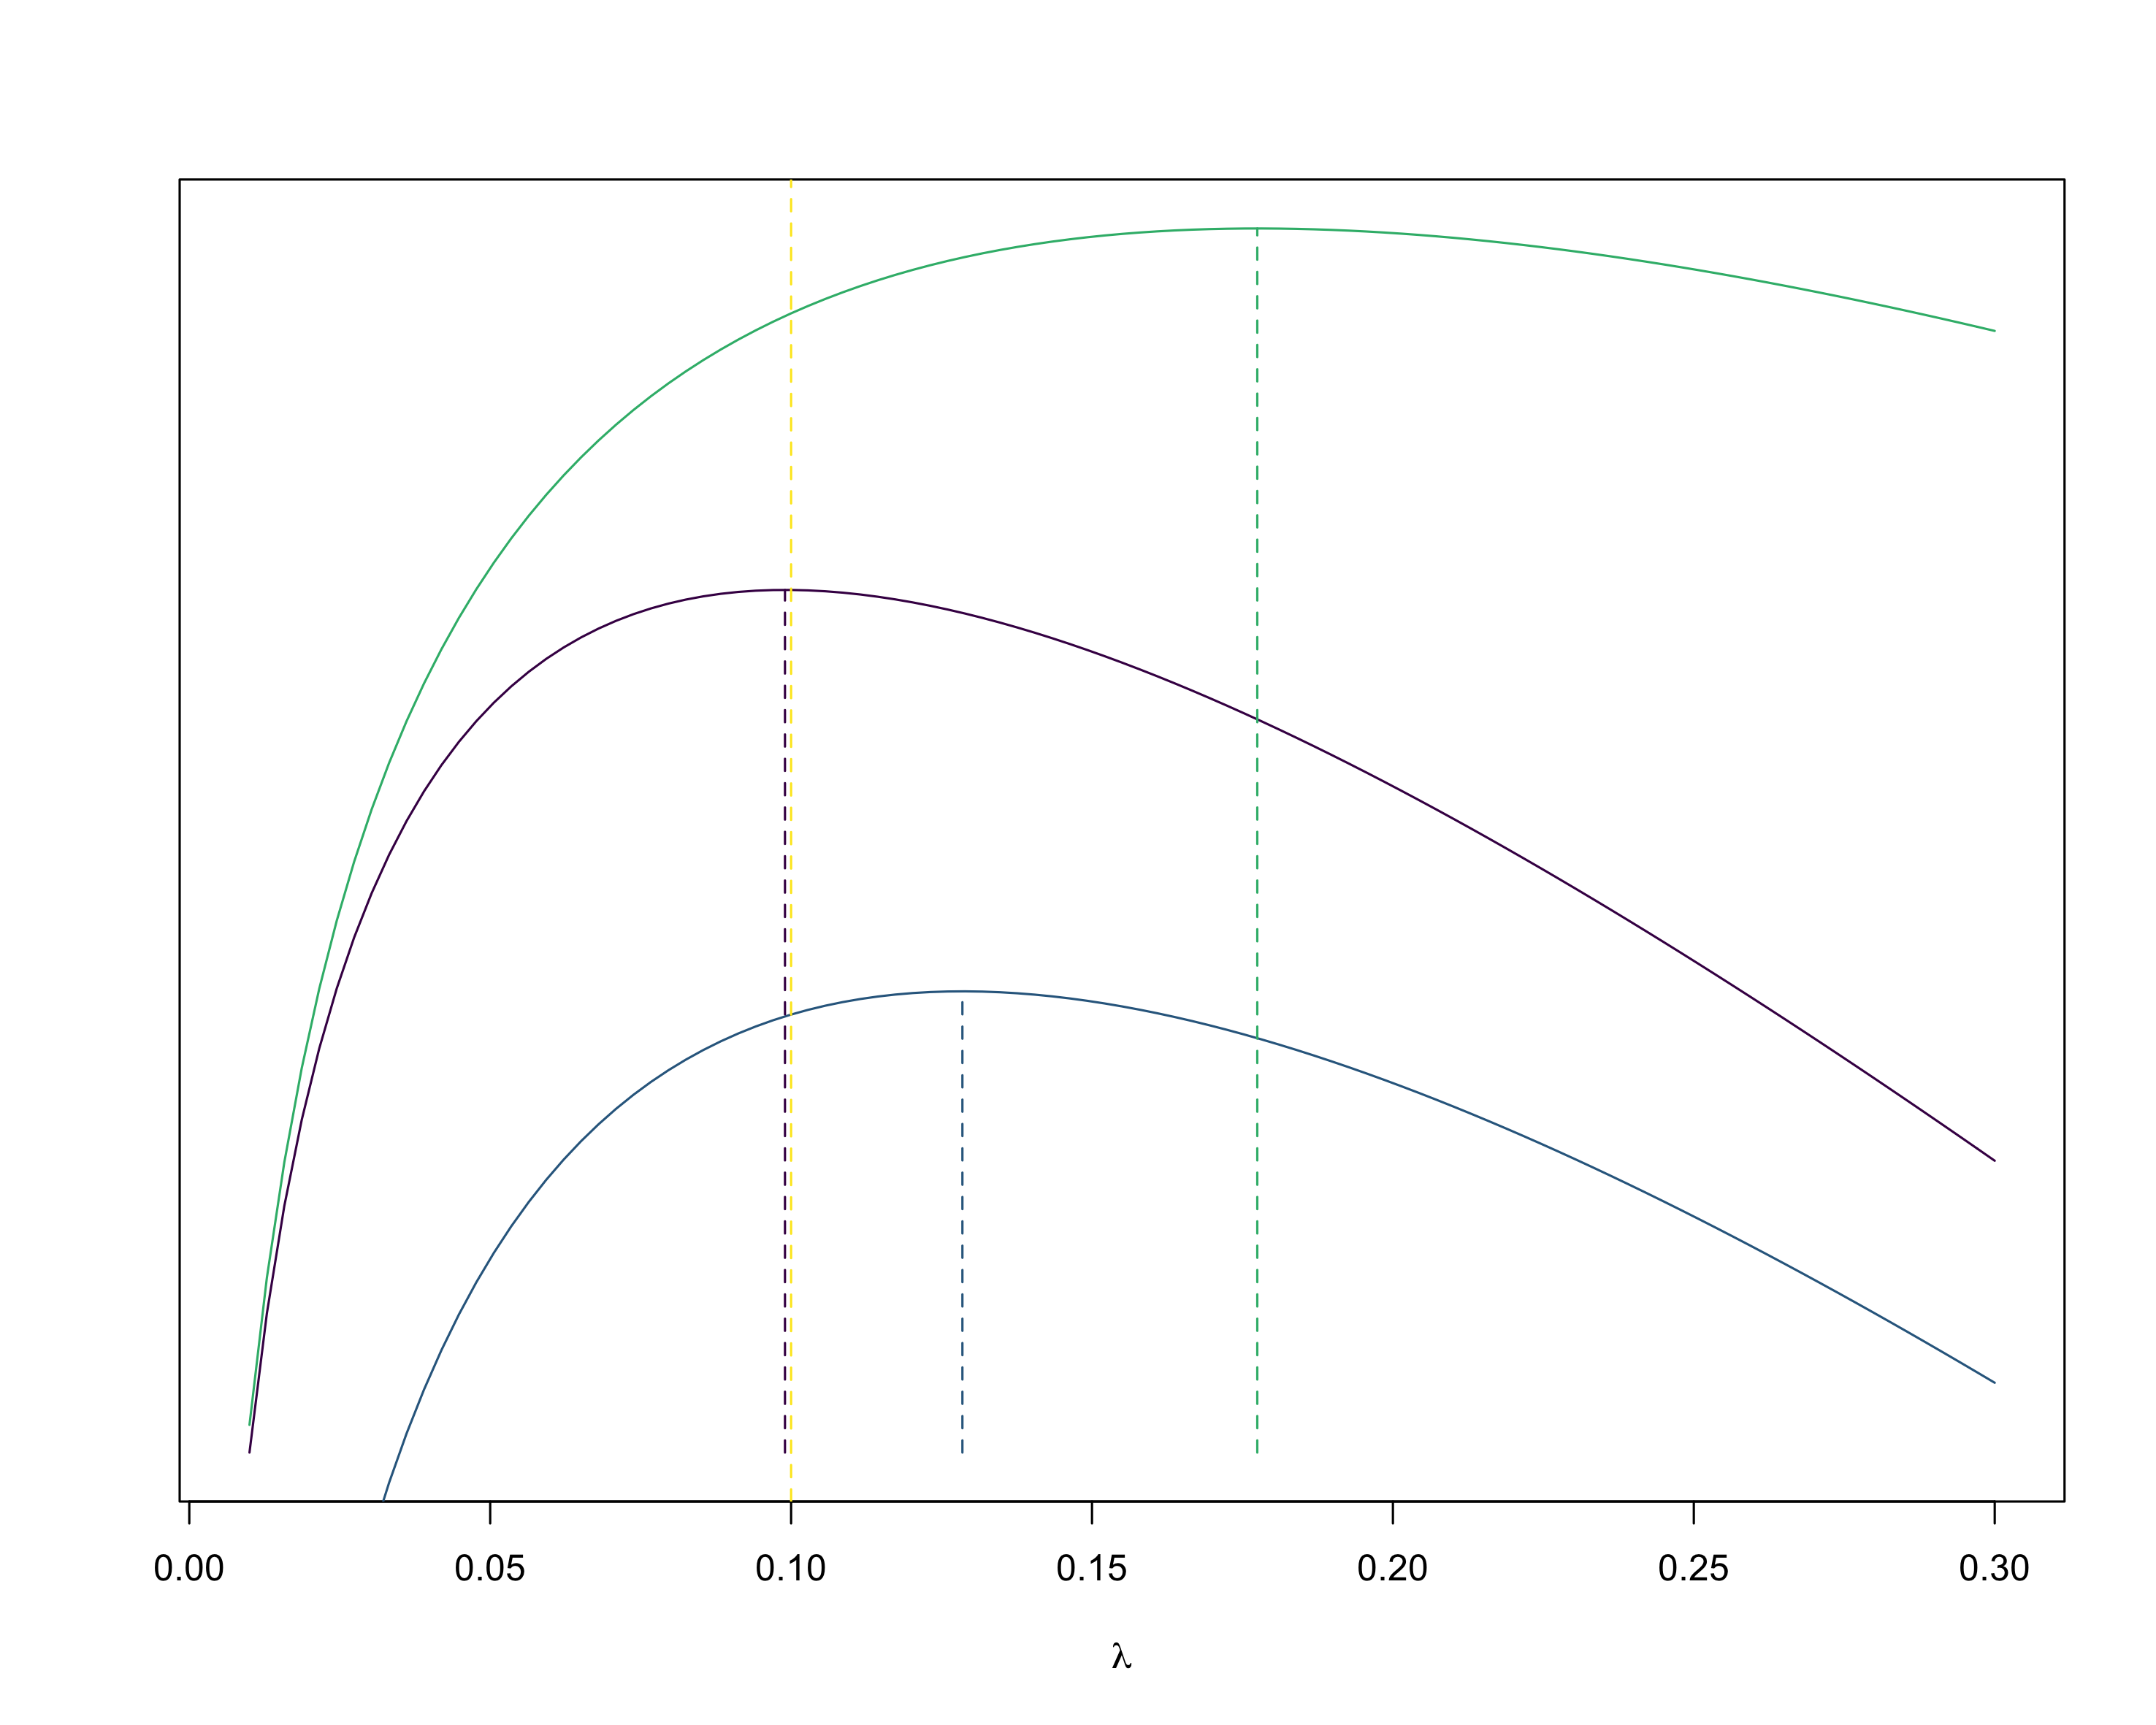
\includegraphics[width=10cm]{likelihood.png}
\caption{$\hat{\lambda}_1$ (morado), $\hat{\lambda}_2$ (azul), $\hat{\lambda}_3$ (verde) con el valor real $\lambda$ (amarillo) y las respectivas funciones de log-verosimilitud.}
\label{fig:lik}
\end{figure}



Se puede apreciar claramente en la figura \ref{fig:lik} que el estimador que incorpora la información de censura es el más cercano al valor real. El estimador $\hat{\lambda}_2$ sobrestima el valor real del parámetro ya que se están tomando como exactos los datos censurados por la derecha (recordemos que $E[T] = 1/\lambda$), mientras que el estimador $\hat{\lambda}_3$ está descartando todos los valores $t_i > 15$, por lo que el parámetro también es sobrestimado. El código para reproducir este ejemplo se puede encontrar en el apéndice \ref{ap:lik}.

\citet{kaplan-meier} introdujeron una de las técnicas más utilizadas en el análisis de supervivencia, el estimador producto-límite, también conocido como el \textbf{estimador Kaplan-Meier}. Este estimador permite aproximar funciones de supervivencia en presencia de observaciones exactas y censuradas por la derecha. El estimador Kaplan-Meier es un estimador no paramétrico de la función de supervivencia, es decir, no depende de suponer una familia específica para la distribución de los tiempos de fallo. Si la variable de interés es continua, el estimador producto-límite es
\begin{equation}
\label{eq:km}
\hat{S}(t) = \prod_{i: t_i \leq t} \left( 1-\frac{d_i}{n_i}\right),
\end{equation}
donde $d_i$ es el número de tiempos de falla iguales a $t_i$ y $n_i$ es el número de individuos en riesgo al tiempo $t_i$, por lo que el estimador Kaplan-Meier es una función escalonada con saltos en cada tiempo de falla exacto. Además, es el estimador de máxima verosimilitud para $S$.

 \begin{table}[htb]
\begin{lstlisting}
library(survival)

dt_aml <- survival::aml

times <- Surv(dt_aml$time, dt_aml$status)
km2 <- survfit(times ~ dt_aml$x, conf.type = "none")

plot(km2, lwd = 1.5, conf.int = FALSE, col = c("forestgreen", "darkorange"))
\end{lstlisting}
\caption{Código para obtener los estimadores Kaplan-Meier en R.}
\label{cod:km}
\end{table}

 En R se puede calcular el estimador producto-límite utilizando la función \texttt{survfit} del paquete \texttt{survival}, ver \citet{survival-book}. Se presenta un ejemplo utilizando el conjunto de datos \texttt{aml} del mismo paquete. La base \texttt{aml} cuenta con información sobre 23 pacientes que padecen leucemia mieloide aguda. De estos 23 individuos, 18 presentaron el evento de falla (muerte) en el tiempo de estudio y 5 son censurados por la derecha. Además se tiene una variable adicional que indica si el paciente recibió ciclos adicionales de quimioterapia. El interés del estudio era analizar si estos ciclos adicionales de quimioterapia afectaban la distribución de los tiempos de supervivencia (medidos en semanas). En el cuadro \ref{cod:km} se presenta el código para obtener dos estimadores Kaplan-Meier, uno para los pacientes que recibieron ciclos adicionales de quimioterapia y otro para los que no (figura \ref{fig:km2}). Es interesante notar que el paciente con el mayor tiempo de fallo ($t = 161$ semanas) presenta censura por la derecha, por lo que los estimadores producto-límite que involucran a este individuo nunca caen a cero.
 
 \begin{figure}[hbt]
\centering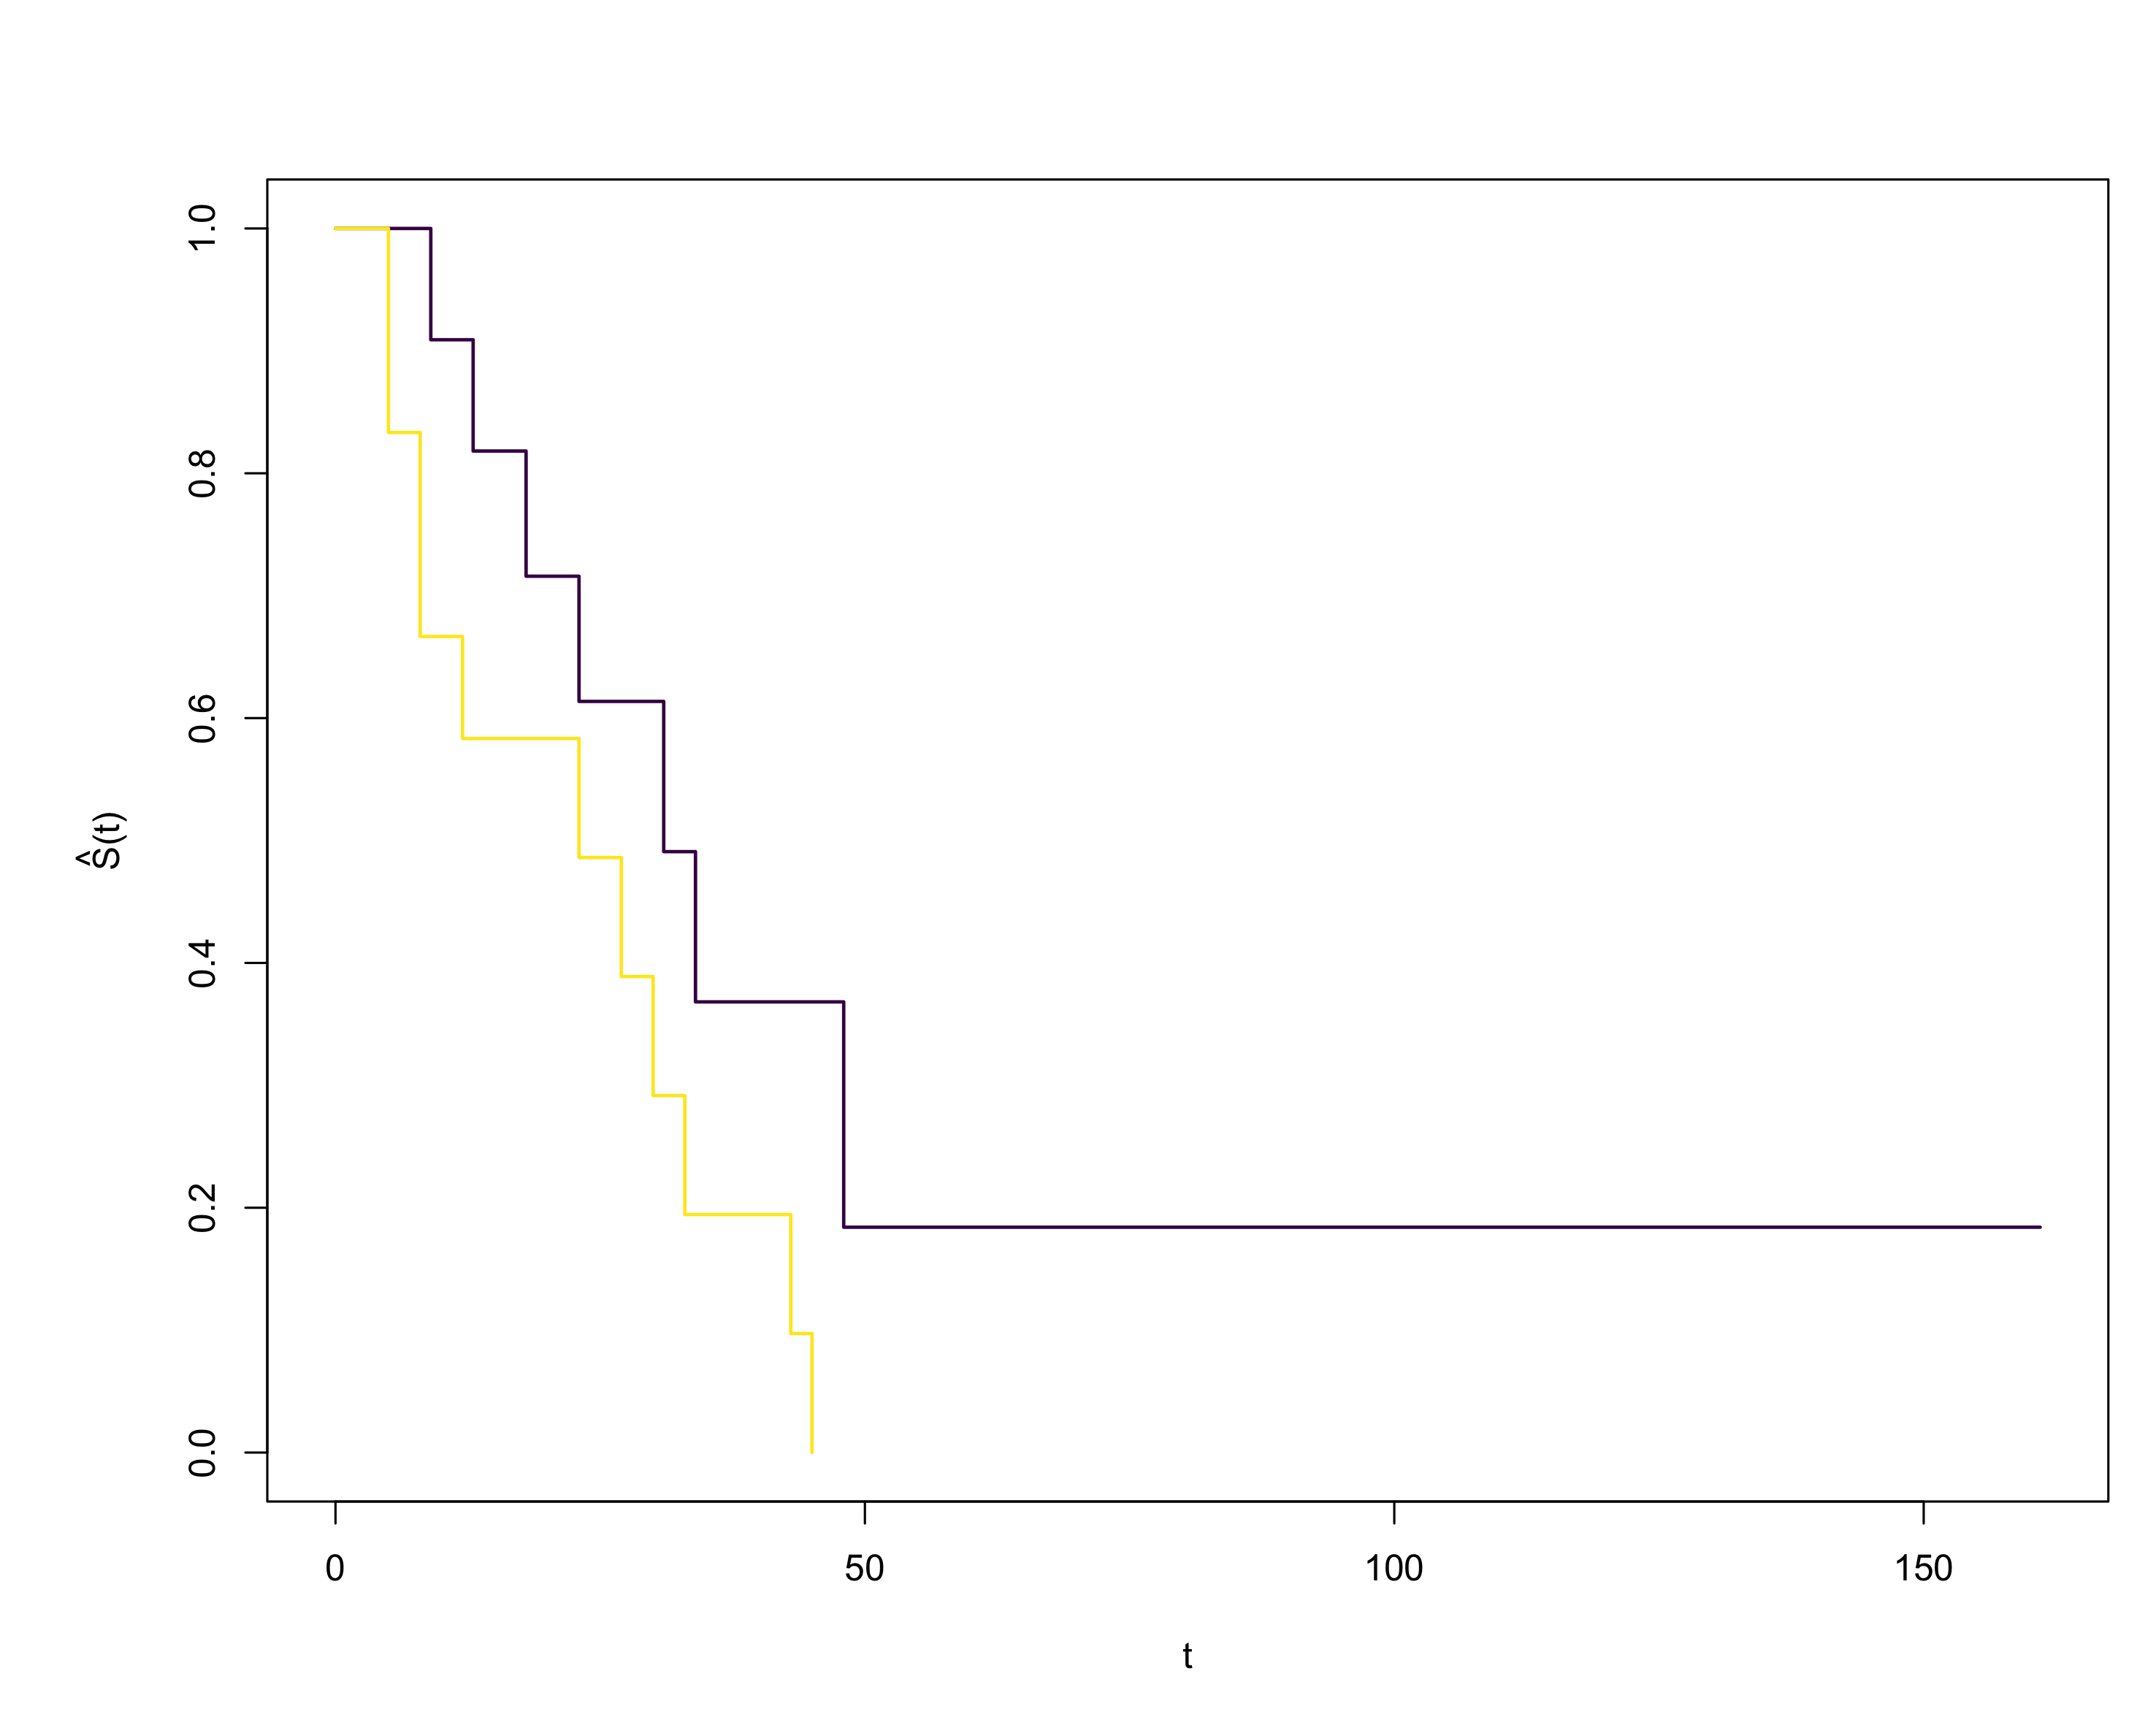
\includegraphics[width=9cm]{km2.png}
\caption{Estimadores Kaplan-Meier para los 11 pacientes que recibieron ciclos adicionales de quimioterapia (morado) y para los 12 que no (amarillo).}
\label{fig:km2}
\end{figure}

La figura \ref{fig:km2} parece indicar que los pacientes que recibieron ciclos adicionales de quimioterapia tienen un aumento importante en la función de supervivencia. Para sustentar esta evidencia visual se podrían calcular intervalos de confianza sobre los estimadores o una prueba de hipótesis sobre la diferencia entre las funciones de supervivencia. Para una explicación más extensa del estimador, ver \citet{kaplan-meier}. En \citet{moore} se puede encontrar más información sobre los intervalos de confianza para el estimador y cómo obtenerlos en R. También se recomienda consultar la documentación de la función \texttt{survfit} en R con el comando \texttt{?survfit}. Finalmente, \citet{klein} contiene más información sobre los intervalos de confianza y las pruebas de hipótesis mencionadas.

\subsection{Modelo de regresión de Cox}
\label{seccion_coxph}
El modelo presentado en \citet{cox} explica cómo describir la función de riesgo de un individuo como función de un vector de variables explicativas y un vector de coeficientes. Para el individuo $j$, sea $z_j\in \mathbb{R}^p$ su vector de covariables. El modelo de Cox consiste en expresar la función de riesgo de este individuo como
\begin{equation} \label{cox_ph}
h_j(t) = h_0(t)e^{z_j^\prime \beta},
\end{equation}
donde la notación $z_j^\prime$ se refiere al vector transpuesto de $z_j$, $\beta\in \mathbb{R}^p$ es el vector de coeficientes y $h_0$ es una función de riesgo base, común a todos los individuos, que describe a un hipotético individuo para el cual $z = 0$. En el caso específico en que $z$ sea una variable indicadora para distinguir un grupo control y un grupo piloto, $h_0$ es la función de riesgo para los individuos en el grupo control y $e^\beta$ es la constante por la cual se multiplica la función de riesgo de los individuos en el grupo piloto.

Es común encontrar este modelo en la literatura bajo el nombre de \textbf{modelo de riesgos proporcionales de Cox}, pero este nombre solamente es aplicable a un caso específico de los que se consideran en \citet{cox}. Específicamente, si se cumple que el vector de covariables no depende del tiempo, entonces se tiene que para dos individuos $i, j$
\begin{align}
\label{eq:prop_haz}
\frac{h_j(t)}{h_i(t)} &= \frac{h_0(t)\exp (z_j^\prime \beta)}{h_0(t)\exp (z_i^\prime \beta)} \nonumber \\
&= \exp ((z_j-z_i)^\prime \beta),
\end{align}
que es una constante como función del tiempo. Además, tomando logaritmo de ambos lados se tiene que
$$\log \left(\frac{h_j(t)}{h_i(t)}\right) = z^{*\prime} \beta,$$ donde $z^* = z_j-z_i$. Esto es un modelo lineal en los parámetros para el logaritmo de la razón de tasas de riesgo.

Es importante hacer énfasis en que el supuesto de proporcionalidad entre las funciones de riesgo se debe cumplir para utilizar el modelo con covariables independientes del tiempo. Sin embargo, el autor señala que se puede introducir esta dependencia del tiempo para describir comportamientos distintos a la multiplicación de las tasas de riesgo. En ese caso el modelo queda de la forma
\begin{equation*}
h_j(t) = h_0(t)e^{z_j(t)^\prime \beta}.
\end{equation*}

También en \citet{cox} se presenta el método de \textit{verosimilitud condicional} para la estimación de los coeficientes sin hacer supuestos sobre la función de riesgo base $h_0$. En la literatura es común encontrar este mismo método bajo el nombre de \textit{verosimilitud parcial}. Estos nombres se deben a que \textit{"los intervalos de tiempo en que no se presentan fallas no aportan información sobre $\beta$, ya que en estos intervalos bien podría pasar que $h_0$ sea idéntica a cero"}. Es por esto que el autor obtiene la función de verosimilitud en los tiempos de falla $\lbrace t_{i} \rbrace$, condicionando sobre los individuos en riesgo en ese tiempo, denotados $\mathcal{R}(t_{i})$. Cuando no hay empates en los tiempos de falla, la función de verosimilitud parcial es entonces de la forma
$$\mathcal{L}(\beta) = \prod_{i=1}^n \left(\frac{\exp (z_i^\prime \beta)}{\sum_{l\in \mathcal{R}(t_{i})}\exp (z_l^\prime \beta)}\right).$$ A partir de aquí se puede obtener el estimador de máxima verosimilitud $\hat{\beta}$.

Es importante resaltar que esta forma de la función de verosimilitud se da cuando no hay empate en los tiempos de falla. En teoría, si la variable de interés es continua, que dos eventos se presenten al mismo tiempo es un evento de probabilidad cero. Sin embargo, en la práctica, estos empates se pueden observar debido al redondeo de los tiempos de fallo o a una verdadera naturaleza discreta en la variable de interés. Algunos métodos para lidiar con estos empates son el método marginal, el exacto, el de Breslow y el de Efron. Una explicación breve de estos métodos se puede encontrar en \citet{moore}.

Ahora se presenta una aplicación en R del modelo de riesgos proporcionales utilizando el conjunto de datos \texttt{aml} introducido en la sección \ref{sec:truncados}. La intención es cuantificar el efecto de los ciclos adicionales de quimioterapia sobre las funciones de riesgo de los pacientes. Primero, se transforma la variable explicativa en una variable indicadora, haciendo explícitamente grupo base o control a los pacientes que no recibieron ciclos adicionales de tratamiento.

Antes de ajustar el modelo se debe checar que se cumple la hipótesis de riesgos proporcionales. Para esto, sea $h_0$  la función de riesgo del grupo control y $h_1$ a la del grupo piloto y $S_0$, $S_1$ sus respectivas funciones de supervivencia. Bajo el supuesto de riesgos proporcionales, se tiene que $h_1(t) = h_0(t) e^\beta.$ Utilizando las relaciones entre la función de riesgo y la función de supervivencia introducidas al principio del capítulo \ref{analisis_sup} se sigue que $S_1(t) = S_0(t) ^ {\exp (\beta)}.$ Ahora, tomando logaritmo dos veces y multiplicando por -1 de cada lado, se obtiene
\begin{align*}
S_1(t) = S_0(t) ^ {\exp (\beta)} &\implies \log (S_1(t)) = e^\beta \ \log (S_0(t))\\
&\implies \log (-\log (S_1(t))) = \beta + \log (-\log (S_0(t))).
\end{align*}
Es decir, que si se grafican las funciones $\log (-\log (S_1(t)))$ y $\log (-\log (S_0(t)))$ contra $t$ o $\log (t)$, bajo el supuesto de riesgos proporcionales se deben ver dos líneas paralelas, separadas por $\beta$. La figura \ref{fig:coxph} presenta esta gráfica utilizando los estimadores Kaplan-Meier de la sección \ref{sec:truncados}.

\begin{figure}[htb]
\centering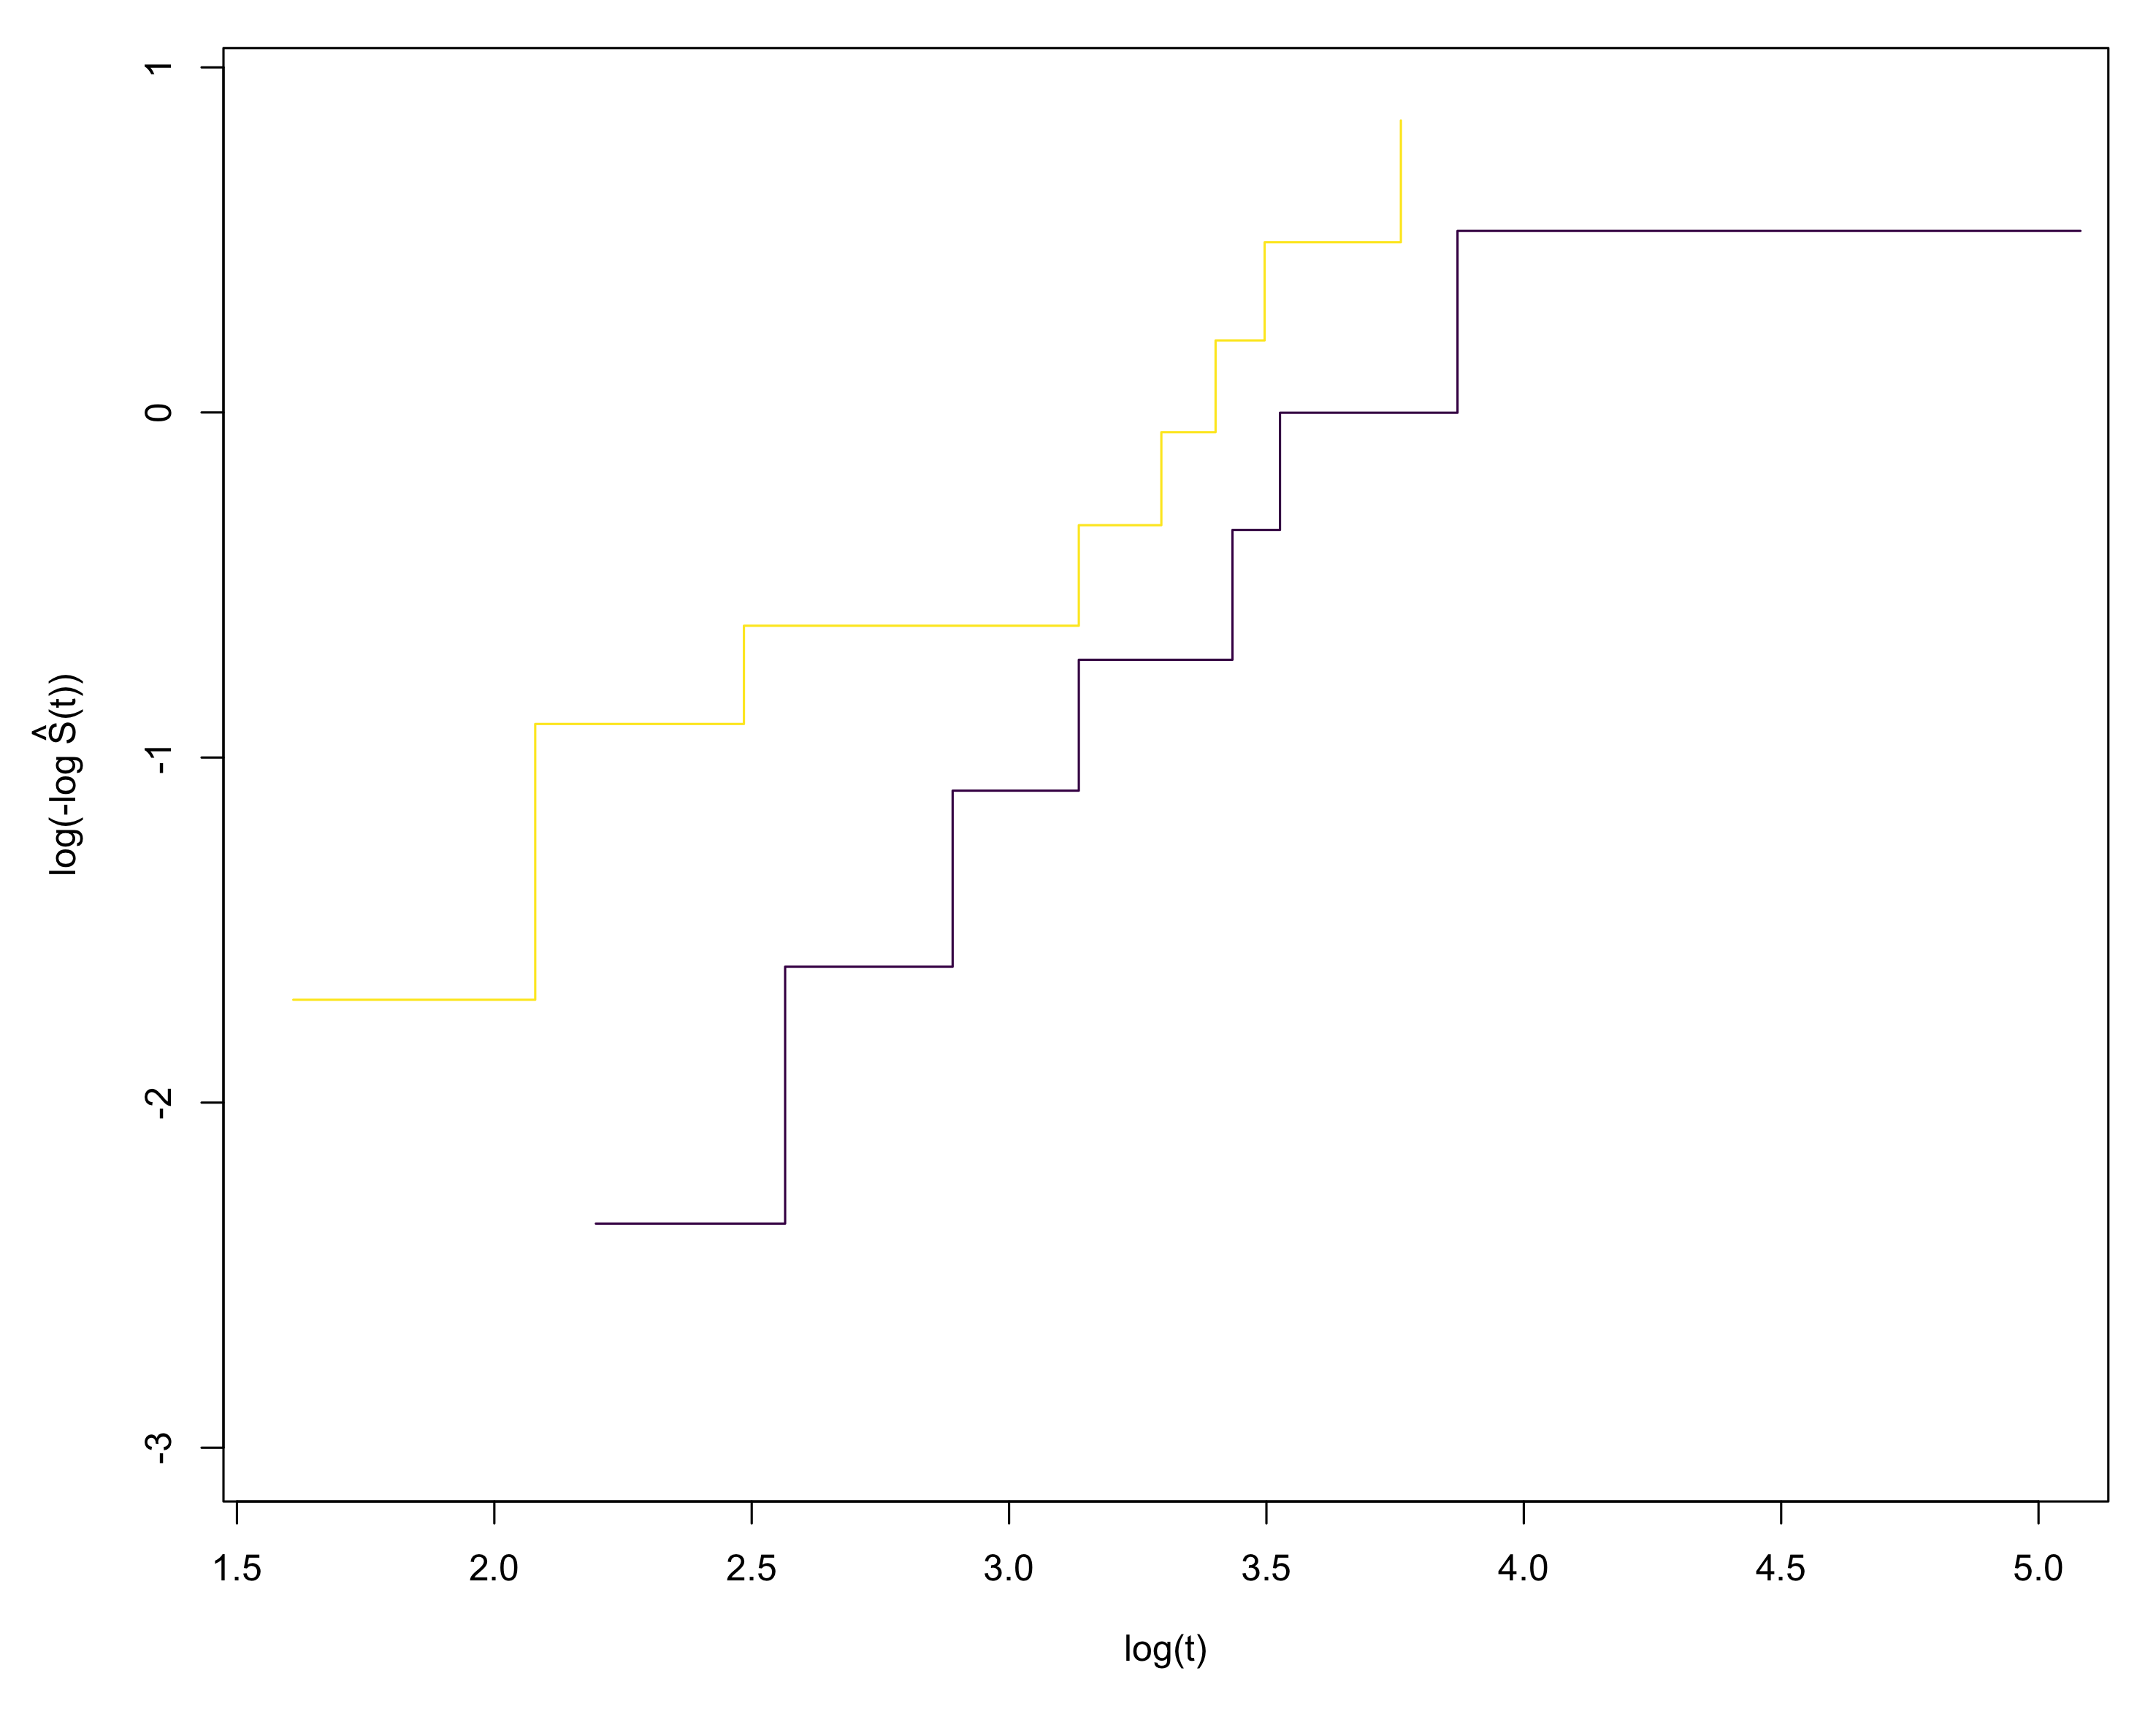
\includegraphics[width=10cm]{prop_haz_km.png}
\caption{Estimadores Kaplan-Meier para el grupo control (amarillo) y piloto (morado). }
\label{fig:coxph}
\end{figure}

Revisando los datos, se puede ver que hay algunos empates en los registros. La documentación de la función \texttt{coxph} señala que estos empates son tratados con el método de Breslow, ya que ``es más preciso y eficiente computacionalmente" \citep{survival-book}. En el cuadro \ref{cod:coxph} se muestra el código para ajustar el modelo.

\begin{table}[htb]
\begin{lstlisting}
library(survival)
library(tidyverse)

dt_aml <- survival::aml

times <- Surv(dt_aml$time, dt_aml$status)

dt_transform <- dt_aml %>%
  mutate(
    z = case_when(
      x == "Maintained" ~ 1,
      x == "Nonmaintained" ~ 0
    )
  )

model <- coxph(times ~ dt_transform$z)
summary(model)
\end{lstlisting}
\caption{Código para utilizar el modelo de riesgos proporcionales en R.}
\label{cod:coxph}
\end{table}

\newpage

El modelo arroja una estimación puntual de $\hat{\beta} = -0.9155$. Por la ecuación \eqref{eq:prop_haz} se tiene que $$\frac{h_1(t)}{h_0(t)} = e^{-0.9155} = 0.4003,$$ es decir, que la tasa de riesgo para el grupo control es aproximadamente 2.5 veces mayor que la del grupo piloto. Este resultado parece indicar una disminución considerable en la tasa de riesgo para los pacientes que reciben ciclos adicionales de quimioterapia.

\newpage

Para un mayor estudio del modelo de riesgos proporcionales se recomienda consultar \citet{cox}. Para mayor información sobre pruebas de hipótesis para los coeficientes o la verosimilitud parcial ver \citet{klein}. Más detalles sobre la implementación en R se pueden encontrar en \citet{moore}.

\newpage
\clearpage

\section{Cópulas y estadística bayesiana}

En este capítulo se complementa la teoría del análisis de supervivencia con una introducción a la teoría de cópulas y a la inferencia bayesiana, ambas necesarias para estudiar el modelo de \citet{nieto}. Primero, en la sección \ref{sec_copulas} se habla sobre qué son las cópulas, para qué sirven y se presentan la tau de Kendall y la rho de Spearman como medidas de concordancia alternativas a la correlación de Pearson. Posteriormente, en la sección \ref{sec:bayesiana} se introduce la inferencia bayesiana como una teoría axiomática de la inferencia estadística, mencionando el contexto histórico en el que surgió y se presenta un ejemplo de estimación puntual resuelto con el enfoque bayesiano.

\label{cap:cop}
\subsection{Cópulas} \label{sec_copulas}

Las cópulas son funciones que se utilizan para construir distribuciones conjuntas a través de sus distribuciones univariadas. También se pueden entender las cópulas como funciones de distribución multivariadas con marginales uniformes en el intervalo unitario $(0,1)$ (denotada $U(0, 1)$), \citep{nelsen}. Formalmente, se tiene la siguiente definición.

\textbf{Definición.} Una cópula $C$ es una función 
\begin{align*}
C: [0,1]\times[0,1]&\to [0,1]\\
(u,v) &\to C(u,v)
\end{align*} tal que:
\begin{enumerate}
\item $\forall \ u,v \in [0,1]$, se tiene que
\begin{itemize}
\item $C (u,0) = C(0,v) = 0$,
\item $C(u,1) = u$,
\item $C(1, v) = v$.
\end{itemize}
\item $\forall \ u_1, u_2, v_1, v_2 \in [0,1]$ tales que $u_1 \leq u_2$ y $v_1 \leq v_2$, se tiene que  $$C (u_1,v_1)+C (u_2,v_2) - C(u_1,v_2) - C(u_2,v_1)\geq 0.$$
\end{enumerate}

Las cópulas se utilizan para modelar la estructura de dependencia entre las componentes de vectores aleatorios. Para poder entender esto, es necesario mencionar cómo se utilizan las cópulas para construir distribuciones conjuntas. El siguiente teorema es, según \citet{copula_modeling}, el resultado más importante de la teoría de cópulas. Su importancia recae en que demuestra la relación que existe entre las cópulas y las funciones de distribución.

\begin{theorem}[Teorema de Sklar]
\label{sklar}
Sea $F$ una función de distribución conjunta con marginales $F_X$ y $F_Y$. Entonces, existe una cópula $C$ tal que $\forall \ x,y \in \R$ $$F(x,y) = C(F_X(x), F_Y(y)).$$ Si $F_X$ y $F_Y$ son continuas, entonces $C$ es única.

De la misma manera, si $C$ es una cópula y $F_X$, $F_Y$ son funciones de distribución univariadas, entonces la función $F$ definida como $$F(x, y) = C(F_X(x), F_Y(y))$$ es una función de distribución conjunta con marginales $F_X$ y $F_Y$.
\end{theorem}

La demostración de este teorema se puede encontrar en \citet{nelsen}. 

Dos importantes conclusiones se derivan directamente del Teorema de Sklar. Primero, si se tienen observaciones de un vector bivariado $(X, Y)$ con distribuciones marginales continuas, el Teorema de Sklar dice que la cópula correspondiente a su distribución conjunta es única. Por lo tanto, es útil estimarla a partir de datos disponibles para poder modelar la estructura de dependencia entre $X$ y $Y$. Por otro lado, el teorema de Sklar es una herramienta para crear distribuciones conjuntas con la estructura de dependencia que más convenga a cierta aplicación. En específico, si se tienen distribuciones marginales $F_X$ y $F_Y$, junto con una estructura de dependencia modelada a través de una cópula $C$, entonces se puede crear una función de distribución conjunta que refleje esta estructura utilizando $F(x, y) = C (F_X(x), F_Y(y))$.

Un caso singular de las estructuras de dependencia mencionadas es cuando las componentes de un vector aleatorio son independientes. La forma más común de estudiar relaciones entre las componentes es con el coeficiente de correlación de Pearson, el cual solamente cuantifica la dependencia lineal entre variables. Esto significa que si las componentes son independientes, entonces el coeficiente de correlación vale cero. Sin embargo, un coeficiente de correlación cero no implica independencia entre las componentes (ver figura \ref{fig:panel_corr}). En contraste con el coeficiente de correlación, la teoría de cópulas tiene una forma única de modelar independencia entre las componentes de un vector aleatorio. El teorema \ref{independencia} muestra cómo se modela esta independencia con una cópula específica.

\begin{theorem}
\label{independencia}
Sean $X$ y $Y$ dos variables aleatorias continuas con función de distribución conjunta $F$ y marginales $F_X$ y $F_Y$ respectivamente. Entonces $X$ y $Y$ son independientes si y solo si $C = \Pi$, donde $\Pi$ es la cópula producto dada por $\Pi (u,v) = uv.$
\end{theorem}

\begin{proof}\mbox{}\\*
$\implies\big)$ Si $X$ y $Y$ son independientes, entonces
\begin{equation} \label{conjunta}
F(x, y) = F_X(x)F_Y(y).
\end{equation}

Por el teorema \ref{sklar}, como $F_X$ y $F_Y$ son continuas, se sabe que existe una única cópula $C$ tal que
\begin{equation} \label{copula}
F(x, y) = C(F_X(x), F_Y(y)).
\end{equation}

Juntando \eqref{conjunta} y \eqref{copula} se tiene que $C(F_X(x), F_Y(y)) = F_X(x)F_Y(y)$, por lo que $C = \Pi$.
\newpage
$\impliedby \big)$ Por el teorema \ref{sklar} existe una única $C$ tal que $F(x, y) = C(F_X(x), F_Y(y))$. Si $C = \Pi$ se tiene que $F(x, y) = F_X(x)F_Y(y)$, es decir, $X$ y $Y$ son independientes.
\end{proof}

Como en análisis de supervivencia es común trabajar con la función de supervivencia conjunta en vez de la distribución, se introduce el concepto de cópulas de supervivencia. Se quiere ahora una función $\widehat{C}$ tal que
\begin{equation} \label{suvcop}
S(x, y) = \widehat{C}(S_X(x), S_Y(y)),
\end{equation}
donde $S$ es la función de supervivencia conjunta definida como $$S(x, y ) = P\left( X>x, Y>y\right)$$ y $S_X$ y $S_Y$ son las funciones de supervivencia marginales. El siguiente resultado muestra cómo construir la función $\widehat{C}$ a partir de una cópula $C$. La demostración se puede encontrar en \citet{nelsen}.

\begin{proposition}[Cópulas de supervivencia]
\label{def_cop_surv}
Sean X y Y dos variables aleatorias con distribuciones marginales $F_X$ $F_Y$ y cópula $C$. Entonces, la función $\widehat{C}$ definida como $$\widehat{C}(u, v) = u + v - 1 + C(1-u, 1-v)$$ cumple la ecuación \eqref{suvcop}.
\end{proposition}

Antes de introducir medidas de concordancia alternativas a la correlación de Pearson, se muestra un ejemplo de la necesidad de medidas alternativas para ver relaciones no lineales. Este ejemplo es tomado de \citet{copula_modeling} y consiste en simular un vector aleatorio $X = (X_1, X_2)$ donde $X_1 \sim \mathcal{N}(0, 1)$ y $$X_2 = \begin{cases}
X_1  \text{ con probabilidad } 0.5,\\
-X_1 \text{ con probabilidad }  0.5.
\end{cases}$$ El diagrama de dispersión se muestra en la figura \ref{fig:panel_corr}. Se presenta también un diagrama de dispersión para un vector bivariado con componentes normales estándar generadas de manera independiente. El código para generar las simulaciones se muestra en el cuadro \ref{cod:sim_ejemplo}.

\begin{figure}[H]
    \centering
    \begin{subfigure}[t]{0.45\textwidth}
        \centering
        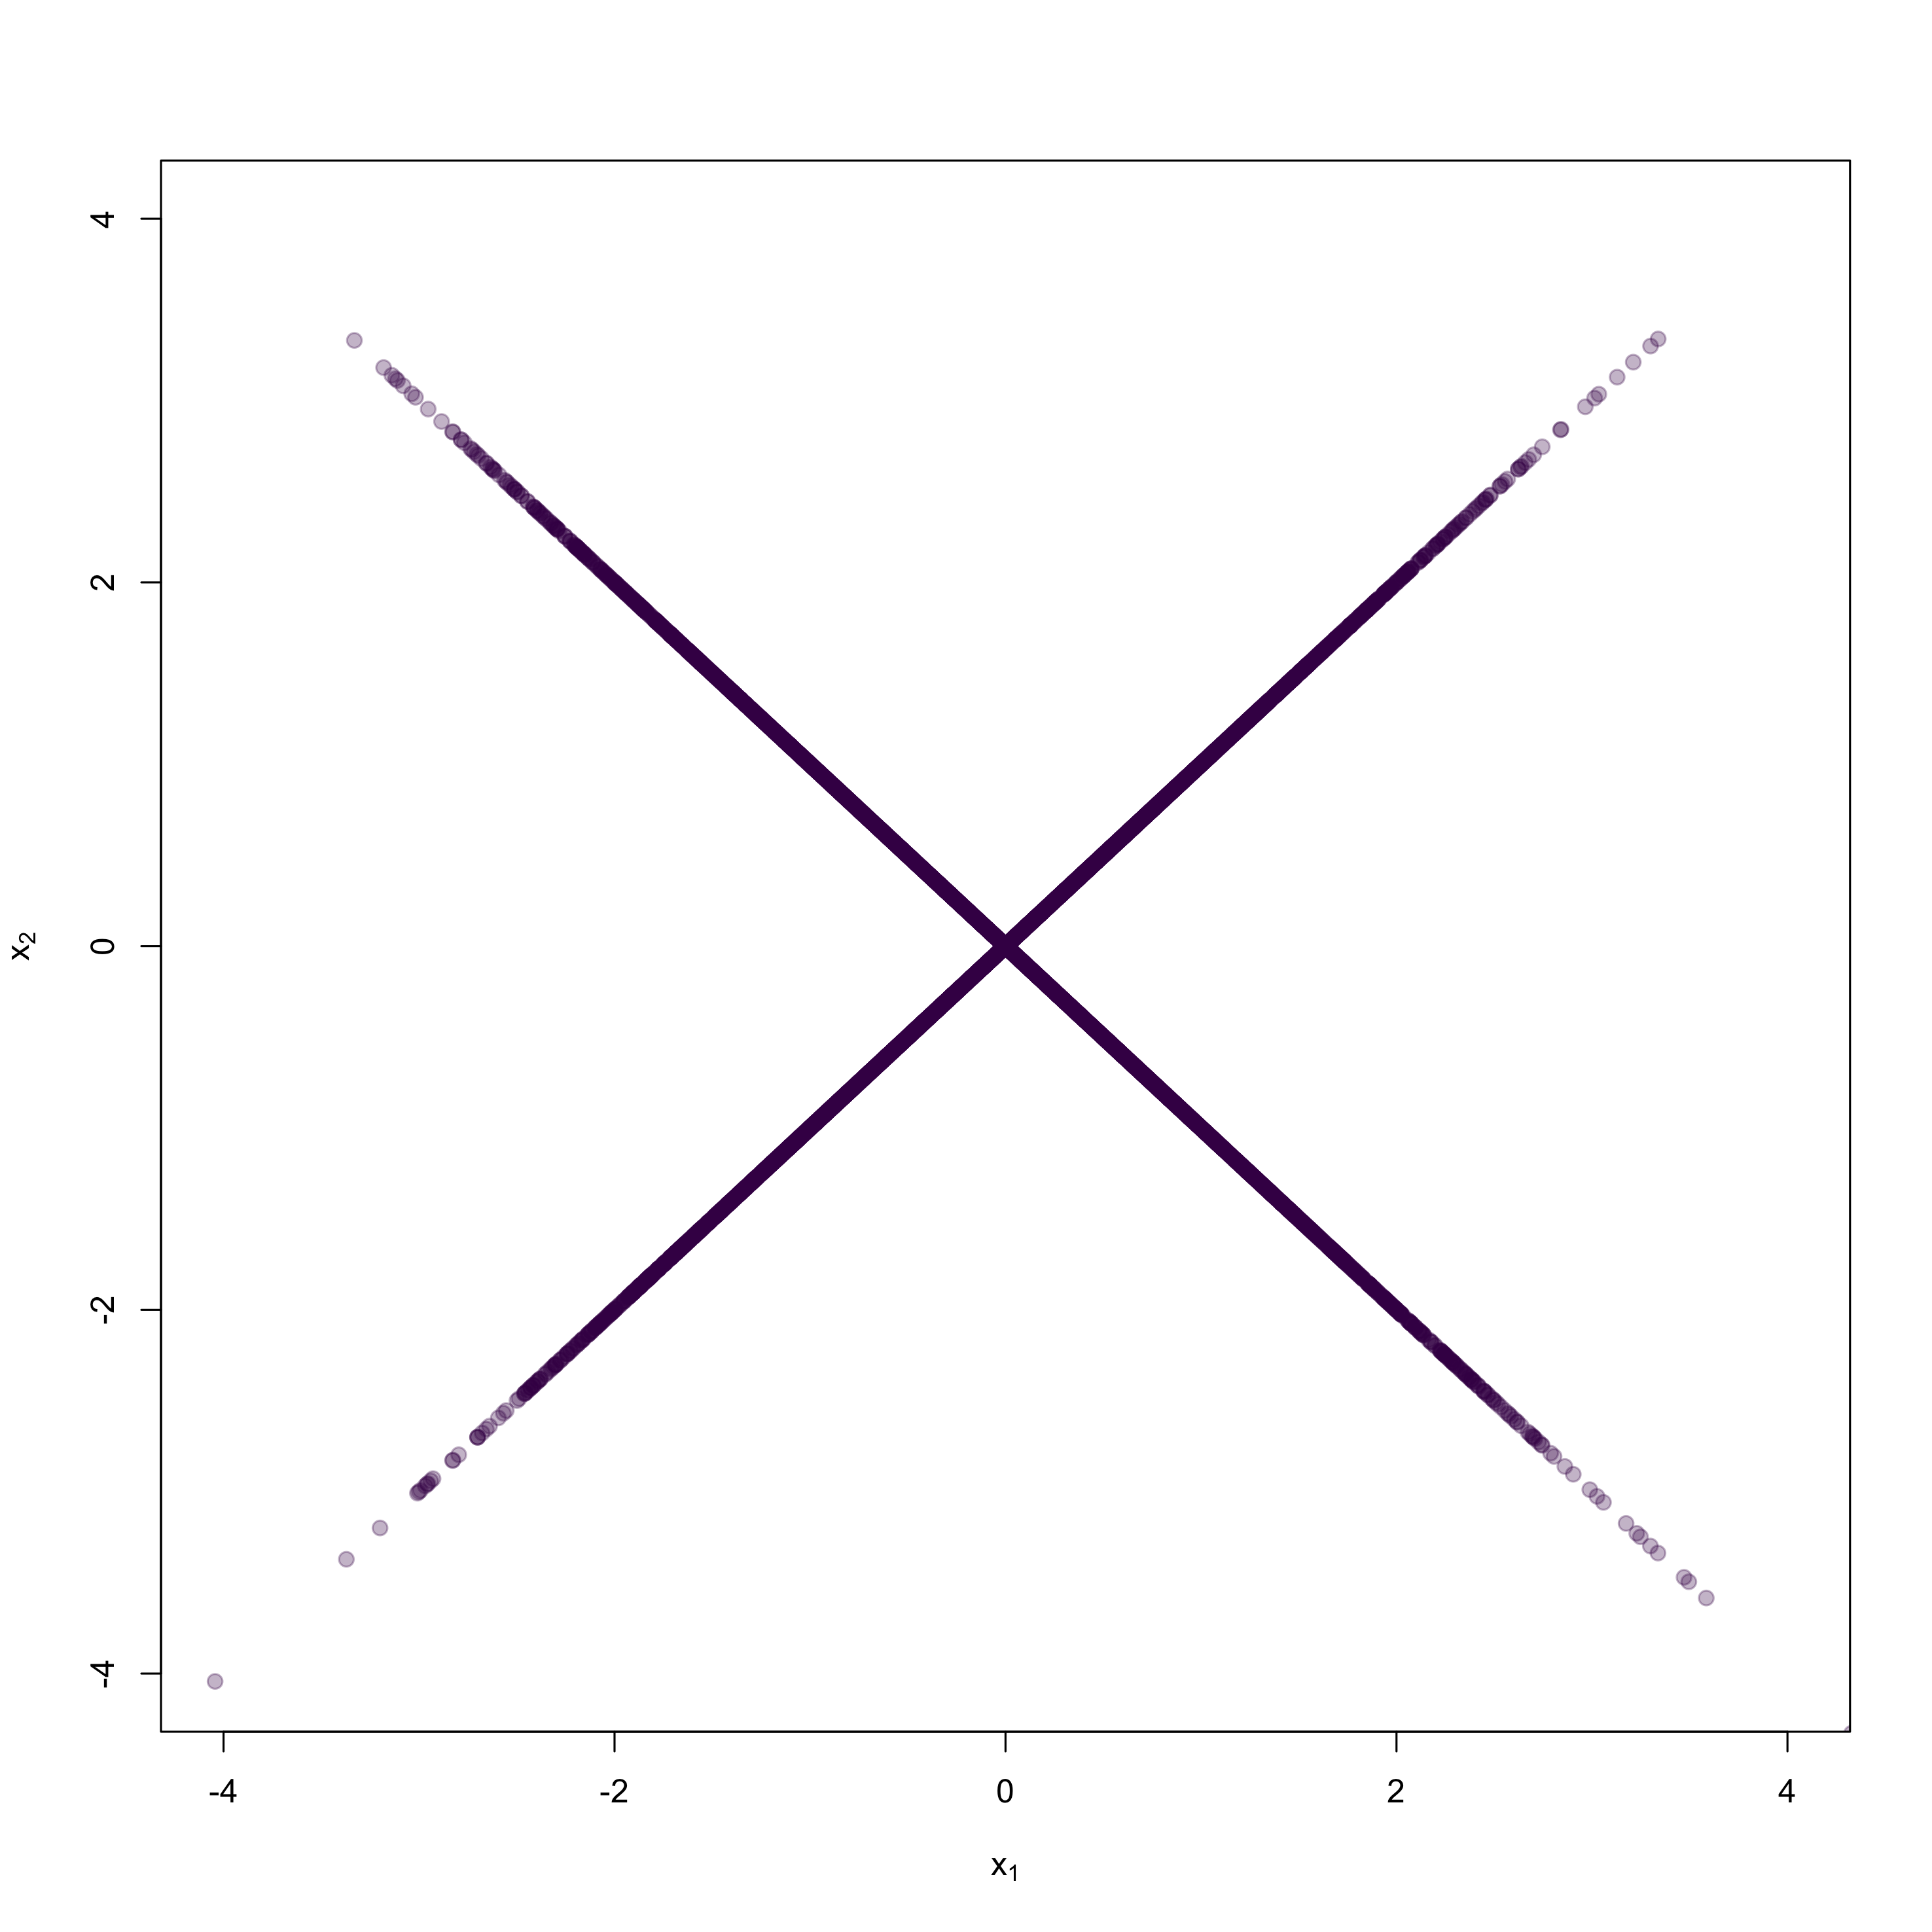
\includegraphics[width=\linewidth]{correlation.png} 
        \caption{Diagrama de dispersión para valores simulados de $(X_1, X_2)$.} \label{fig:corr1}
    \end{subfigure}
    \hfill
    \begin{subfigure}[t]{0.45\textwidth}
        \centering
        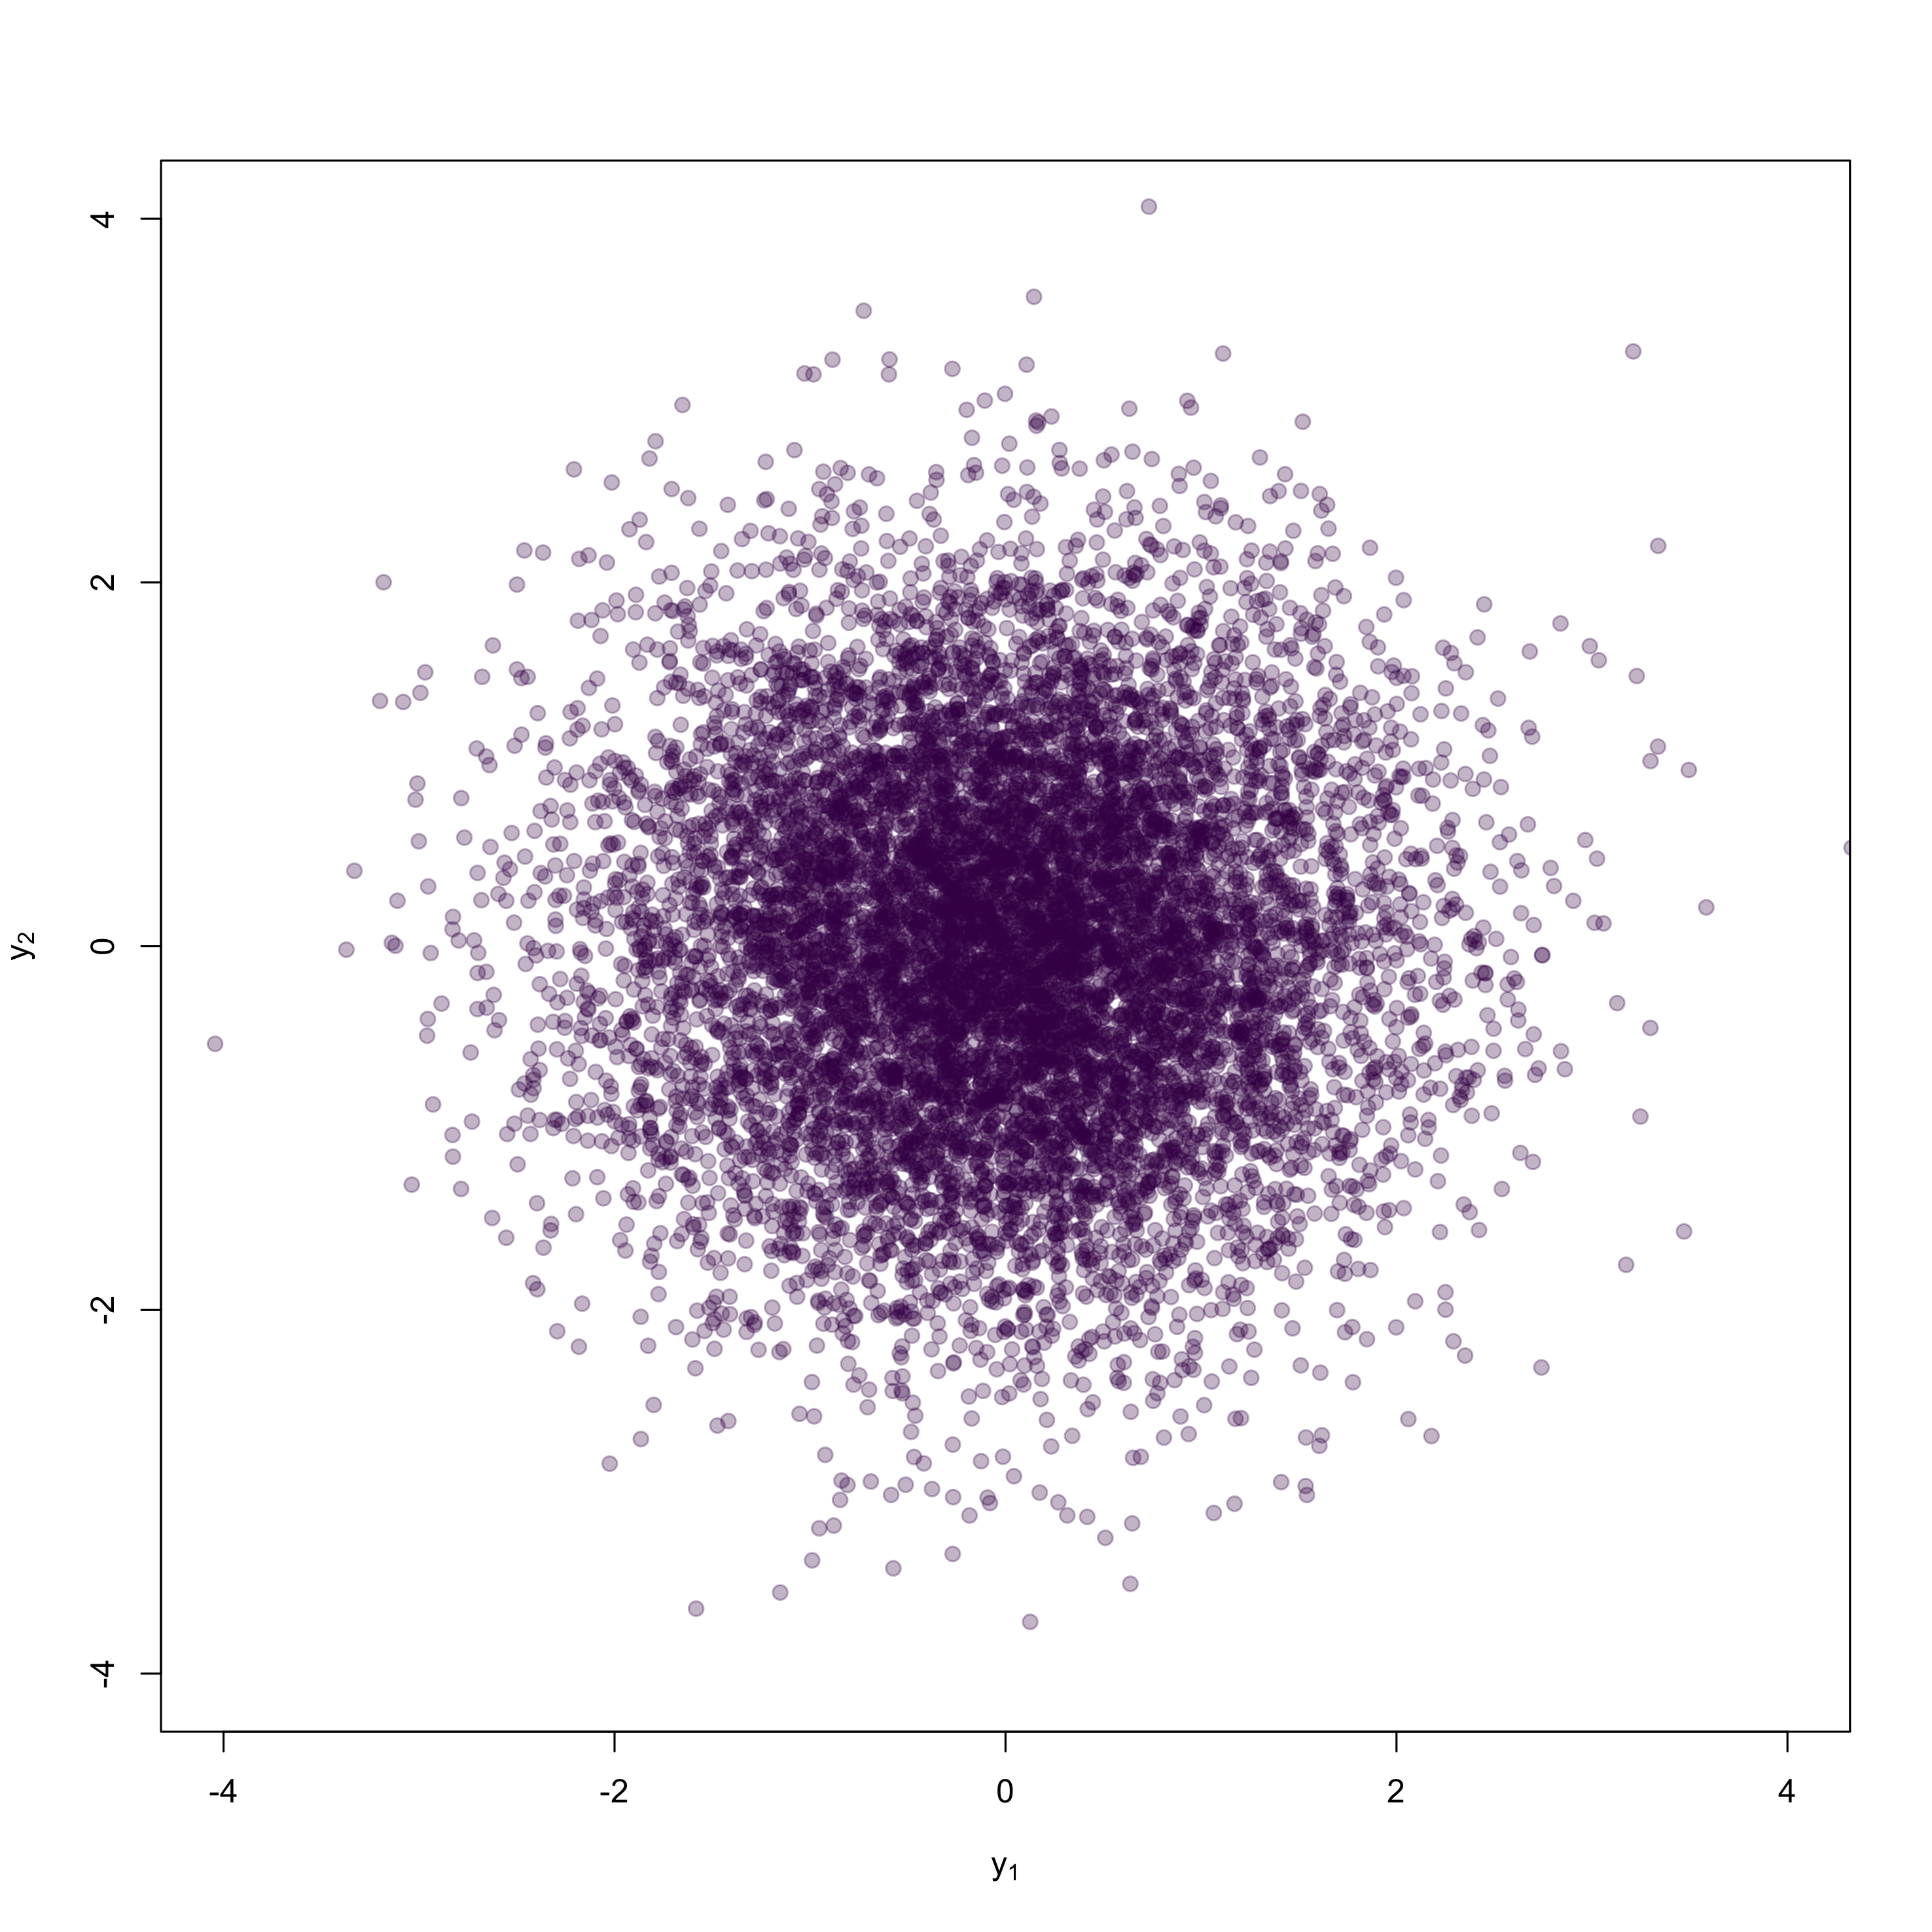
\includegraphics[width=\linewidth]{correlation_ind.png} 
        \caption{Diagrama de dispersión para valores simulados de $(Y_1, Y_2)$ independientes.} \label{fig:corr2}
    \end{subfigure}
    
    \caption{Simulaciones de vectores aleatorios con marginales $\mathcal{N}(0, 1)$. $\mathtt{cor(x1, x2)} = -0.02$ y $\mathtt{cor(y1, y2)} = -0.01$.}
    \label{fig:panel_corr}
\end{figure}

\begin{table}[htb]
\begin{lstlisting}
n.sim <- 1e4

set.seed(42)
x1 <- rnorm(n.sim)
u <- runif(n.sim)
x2 <- ifelse(u <= 0.5, x1, -x1)
y <- rnorm(n.sim)

cor(x1, x2)
cor(x1, y)
\end{lstlisting}
\caption{Código para generar las simulaciones de $(X_1, X_2)$ y $(Y_1, Y_2)$ en R.}
\label{cod:sim_ejemplo}
\end{table}

Viendo la figura \ref{fig:panel_corr}, es claro que las componentes del vector $(X_1, X_2)$ tienen una estructura de dependencia completamente distinta a las componentes del vector $(Y_1, Y_2)$. Sin embargo, ambos valores estimados del coeficiente de correlación de Pearson son parecidos y muy cercanos a cero. Se tomó este ejemplo porque ilustra de gran manera que el coeficiente de correlación no determina la estructura de dependencia y resalta la importancia de visualizar los datos con los que se va a trabajar.

\subsubsection*{Tau de Kendall}
\textbf{Definición.} Sean $(X_1, Y_1)$ y $(X_2, Y_2)$ dos vectores aleatorios independientes e idénticamente distribuidos, con función de distribución $F$. Se define la tau de Kendall, denotada $\uptau_{XY}$, como $$\uptau_{XY} = P\left((X_1-X_2)(Y_1-Y_2)>0\right) - P\left((X_1-X_2)(Y_1-Y_2)<0\right).$$

Un valor más grande de $\uptau_{XY}$ significa que es más probable que un par de observaciones del vector aleatorio $(X, Y)$ sea concordante, es decir, que valores `grandes' de $X$ vienen acompañados de valores `grandes' de $Y$ o valores `chicos' de $X$ vienen acompañados de valores `chicos' de $Y$. Ahora se enuncian algunas propiedades de la tau de Kendall.

\begin{proposition}
\label{prop:kendall}
Sean $X$ y $Y$ dos variables aleatorias continuas con cópula $C$. Entonces
$$\uptau_{XY} = 4\int_{0}^1\int_{0}^1C(u, v) \ dC(u, v) - 1.$$ 
\end{proposition}

\begin{proof} Esta prueba es una adaptación de la demostración en \citet{nelsen}.
Por definición, $$\uptau_{XY} = P\left((X_1-X_2)(Y_1-Y_2) > 0\right) - P\left((X_1-X_2)(Y_1-Y_2) < 0\right).$$

Como $P\left((X_1-X_2)(Y_1-Y_2) < 0\right) = 1-P\left((X_1-X_2)(Y_1-Y_2) > 0\right)$, entonces
\begin{equation} \label{tau}
\uptau_{XY} = 2P\left((X_1-X_2)(Y_1-Y_2) > 0\right) - 1.
\end{equation}

Como la distribución conjunta de $X$ y $Y$ es $C(F_X(x), F_Y(y))$, se puede evaluar esta probabilidad en términos de $C$:
\begin{align}  \label{dobleprob}
P\left((X_1-X_2)(Y_1-Y_2) > 0\right) = &P\left(X_1<X_2, Y_1<Y_2\right) \nonumber \\
&+ P\left(X_2<X_1, Y_2<Y_1\right).
\end{align}

\begin{align*}
P\left(X_1 < X_2, Y_1 < Y_2\right) &=\\
\int_{\Omega_X} \int_{\Omega_Y} P\left(X_1 < X_2, \right. & \left. Y_1 < Y_2 | X_2 = x, Y_2 = y\right) \ dC(F_X(x), F_Y(y))\\
= &\int_{\Omega_X} \int_{\Omega_Y} P\left(X_1 < x, Y_1 < y\right) \ dC(F_X(x), F_Y(y))\\
= &\int_{\Omega_X} \int_{\Omega_Y} C(F_X(x), F_Y(y)) \ dC(F_X(x), F_Y(y))\\
= &\int_0^1 \int_0^1 C(u, v) \ dC(u, v)
\end{align*}
donde $\Omega_X$ y $\Omega_Y$ denotan el soporte de $X$ y $Y$ respectivamente y la última igualdad se obtiene con las transformaciones $u = F_X(x)$ y $v = F_Y(y)$.

De la misma manera, condicionando sobre $X_1, Y_1$ se obtiene que $$P\left(X_2 < X_1, Y_2 < Y_1\right) = \int_0^1 \int_0^1 C(u, v) \ dC(u, v).$$

Sustituyendo estas expresiones en \eqref{dobleprob} y \eqref{tau} se concluye la prueba. Una explicación sobre el diferencial $dC(u, v)$ se incluye en el apéndice \ref{densidad_copula}.
\end{proof}

Con el resultado anterior, se pueden demostrar las siguientes propiedades de $\uptau_{XY}$ \citep{nelsen}:

\begin{enumerate}
\item Si $X$ y $Y$ son independientes, $\uptau_{XY} = 0$.
\item $Y = \alpha X$, $\alpha > 0 \implies \uptau_{XY} = 1$.
\item $Y = \beta X$, $\beta < 0 \implies \uptau_{XY} = -1$.
\end{enumerate}

\newpage

\subsubsection*{Rho de Spearman}

\textbf{Definición.} Sean $X$ y $Y$ dos variables aleatorias con marginales $F_X$ y $F_Y$. Tomando las transformaciones $U = F_X(X)$ y $V = F_Y(Y)$, se define la \textit{rho de Spearman}, denotada $\rho_{XY}$, como
\begin{equation} \label{rho}
\rho_{XY} = \frac{cov(U, V)}{\sqrt{var(U)}\sqrt{var(V)}}.
\end{equation}

La definición \eqref{rho} es el coeficiente de correlación de Pearson entre $F_X(X)$ y $F_Y(Y)$. Si además $X$ y $Y$ tienen cópula $C$, entonces las siguientes definiciones son equivalentes a \eqref{rho}:

\begin{align}
\rho_{XY} &= 12\int_0^1 \int_0^1 C(u, v) \ dudv-3,\nonumber \\
\rho_{XY} &= 12\int_0^1 \int_0^1 uv \ dC(u,v)-3, \nonumber \\
\rho_{XY} &= 12\int_0^1\int_0^1 \left[ C(u, v) - uv \right] dudv \label{volumen}.
\end{align}

Utilizando la ecuación \eqref{volumen}, se puede ver a $\rho_{XY}$ como una `distancia promedio' entre la distribución de $X$ y $Y$, representada por la cópula $C$, y la independencia representada por la cópula $\Pi$.

Al igual que $\uptau_{XY}$, $\rho_{XY}$ cumple las siguientes propiedades:

\begin{enumerate}
\item Si $X$ y $Y$ son independientes, $\rho_{XY} = 0$,
\item $Y = \alpha X$, $\alpha > 0 \implies \rho_{XY} = 1$,
\item $Y = \beta X$, $\beta < 0 \implies \rho_{XY} = -1$.
\end{enumerate}

Para consultar más sobre \textit{métricas de concordancia} con estas propiedades, ver a \citet{nelsen}.

En este trabajo solamente se introducen las dos medidas de concordancia ya mencionadas. La tau de Kendall y la rho de Spearman son útiles ya que ambas se pueden representar por medio de cópulas, sin utilizar la función de distribución conjunta y sin especificar las funciones de distribución marginales.

\subsection{Estadística bayesiana}
\label{sec:bayesiana}
\epigraph{\itshape We owe to the frailty of the human mind one of the most delicate and ingenious of mathematical theories, namely the science of chance or probabilities.}{---Pierre-Simon Laplace, 1776 (Mcgrayne, 2011)}

La estadística bayesiana es una teoría que busca describir cómo deben actuar los individuos en situaciones de incertidumbre para evitar inconsistencias en su comportamiento. Busca establecer métodos para cuantificar incertidumbre y modificarla en presencia de nueva información, así como reglas para la toma de decisiones \citep{bernardo}.  En esta sección se introduce esta teoría axiomática de la inferencia estadística, se presenta brevemente el contexto histórico en el que se desarrolló y un ejemplo de estimación puntual.

Los orígenes de la estadística bayesiana se remontan hasta 1748, cuando el filósofo escocés David Hume publica el libro \textit{Investigación sobre el conocimiento humano} \citep{hume}. En éste, Hume establece que solamente se puede estar seguro de lo que es aprendido por medio de la experiencia. Específicamente cuestiona cómo se entienden las relaciones causa-efecto:

\begin{quotation}
\noindent Al estar determinados por costumbre a trasladar el pasado al futuro en todas nuestras inferencias, cuando el pasado ha sido absolutamente regular y uniforme, esperamos el acontecimiento con la máxima seguridad y no dejamos lugar alguno para la suposición contraria. Pero cuando se ha encontrado que efectos distintos siguen de causas que, al parecer, son exactamente iguales, todos estos efectos distintos han de presentarse a la mente al trasladar el pasado al futuro, y deben entrar en nuestra consideración cuando determinamos la probabilidad del acontecimiento.
\end{quotation}

El escepticismo de David Hume sobre las relaciones causa-efecto fue tratado matemáticamente por Thomas Bayes, quien buscó la manera de describir las probabilidades de las causas a partir de sus efectos observables. Su objetivo fue aproximar la probabilidad de un evento futuro del cual no conocía nada más que su pasado, es decir, regresar de observaciones en el mundo real a sus causas probables. A este problema se le ha conocido como el problema de probabilidad inversa o probabilidad de las causas  (Mcgrayne, 2011).

A pesar de que los orígenes de la estadística bayesiana los encontramos en la Inglaterra de finales del siglo XVIII, el mayor exponente de esta teoría fue el matemático francés Pierre-Simon Laplace. En presencia de grandes cantidades de datos astronómicos obtenidos a lo largo de los años, Laplace se preguntó sobre las posibles causas de las divergencias y errores en las observaciones. A Laplace se le atribuye la versión moderna del célebre Teorema de Bayes. En su forma más simple, este teorema establece que:
\begin{equation}
\label{bayes}
P(C|D) = \frac{P(C)P(D|C)}{P(D)},
\end{equation}
donde, utilizando la terminología del siglo XVIII, $P(C)$ es una creencia sobre la causa $C$ descrita de manera probabilística antes de observar los datos $D$, $P(D|C)$ es la probabilidad de observar los datos bajo la causa $C$ y el lado izquierdo $P(C|D)$ es una descripción probabilística de la creencia en la causa $C$ tras observar los datos $D$.

Es importante notar que se habla de ``creencias'' en las causas. Esto se debe a que en la estadística bayesiana se tiene un concepto de probabilidad distinto a aquél del enfoque frecuentista. En \citet{feller} se habla de la \textit{probabilidad estadística} (frecuentista) como ``un concepto que se refiere a resultados posibles de un experimento conceptual'', esto significa que la probabilidad está únicamente relacionada con la variabilidad observada en realizaciones de un mismo experimento. En contraste, la probabilidad en el sentido bayesiano es una cuantificación de la incertidumbre, sin importar si ésta es producto de la misma variabilidad o de la falta de información (ignorancia) del individuo en cuestión. Por ello se dice que la probabilidad en el sentido bayesiano es una \textbf{probabilidad subjetiva}.

Al principio de esta sección se mencionó que la estadística bayesiana busca describir cómo los individuos deben tomar decisiones en situaciones de incertidumbre. Para entender esta idea, se explica ahora qué es un problema de decisión con incertidumbre y se plantea un problema de inferencia estadística como un problema de decisión con incertidumbre.

\citet{mendoza} definen un problema de decisión como la situación en la que un tomador de decisiones se enfrenta a un conjunto de decisiones, 	de las cuales debe elegir una y solamente una de ellas. Una decisión es juzgada por sus consecuencias y será mejor mientras más satisfacción le produzca al individuo. Además, se dice que un problema de decisión es con incertidumbre cuando para al menos una decisión existen múltiples consecuencias posibles. Un problema de decisión está caracterizado por cuatro elementos:
\begin{itemize}
\item Un conjunto de decisiones $\mathcal{D} = \lbrace d_1, d_2, \dots, d_k\rbrace$.
\item El conjunto de eventos inciertos relevantes. Para cada $d_i \in \mathcal{D}$ se tiene $E_i$, una partición del evento seguro $\Omega$ y se define el conjunto de eventos inciertos relevantes como $\mathcal{E} = \cup_{i=1}^k E_i$.
\item El conjunto de consecuencias. Para cada $d_i \in \mathcal{D}$ se tiene $C_i = \lbrace c_{i1}, c_{i2}, \dots, c_{in_i}\rbrace$, donde $c_{ij}$ es la consecuencia de elegir $i$ y que suceda $j$, y el conjunto de consecuencias se define como $C = \cup_{i=1}^k C_i$.
\item Una relación de preferencia $\succ$ definida sobre los elementos de $\mathcal{D}$.
\end{itemize}

Ya definidos los elementos de un problema de decisión se pueden establecer los axiomas de coherencia, los cuales son la base para esta teoría axiomática de inferencia estadística. Es importante recalcar, como mencionan \citet{bernardo}, que estos axiomas no buscan describir la manera en que los individuos toman decisiones en la realidad, si no que son una serie de principios que un tomador de decisiones debería seguir para evitar inconsistencias en su comportamiento. En el apéndice \ref{ap:bayes} se incluye la versión de los axiomas presentada por \citet{mendoza}, la cual es una versión simplificada de los axiomas presentados en \citet{bernardo}. Una vez establecidos los axiomas, se define la probabilidad subjetiva de un evento relevante $E \in \mathcal{E}$ bajo las condiciones $H$, denotada $P(E|H)$, demuestran que esta probabilidad subjetiva existe y es única para todo evento relevante $E \in \mathcal{E}$ y también demuestran que cumple con los axiomas de Kolmogorov como consecuencia de los axiomas de coherencia (ver apéndice \ref{ap:bayes}).

Como último elemento de la teoría de decisión, se introduce el concepto de funciones de utilidad. Una función de utilidad es una función $u: C \to \mathbb{R}$ tal que $\forall c_1, c_2 \in C$, $c_1 \succ c_2 \iff u(c_1) > u(c_2)$. Una vez que se asignan utilidades al conjunto de consecuencias y probabilidades subjetivas a los eventos relevantes, se puede proceder a resolver el problema de decisión con el mecanismo óptimo derivado de los axiomas de coherencia. Este mecanismo se conoce como el criterio de la utilidad esperada y establece que para cualquier par de decisiones $d_1, d_2 \in \mathcal{D}$, $$ \ d_1 \succ d_2 \iff E_H[u(d_1)] > E_H[u(d_2)],$$ donde $E_H$ es el valor esperado bajo las condiciones $H$ y $u(d)$ se refiere a las utilidades asociadas a las consecuencias posibles de la decisión $d$. Como este criterio es el derivado de los axiomas de coherencia, cualquier otro procedimiento utilizado para solucionar un problema de decisión debe ser equivalente al establecido por los axiomas o se contrapone con éstos.

Ahora se presenta un ejemplo para entender cómo plantear el problema inferencial de estimación puntual como un problema de decisión con incertidumbre y resolverlo con el criterio derivado de los axiomas de coherencia. También se muestra cómo actualizar el conocimiento \textit{a priori} sobre el conjunto de eventos inciertos relevantes $\mathcal{E}$ en presencia de nueva información. Este ejemplo se encuentra en \citet{mendoza}.

Sea $X \sim \mathcal{N}(\mu, \sigma^2)$ con $\sigma^2$ conocida, se busca obtener un estimador $\hat{\mu}$ de $\mu$. Podemos expresar el conjunto de opciones como $\mathcal{D} = \lbrace d_{\hat{\mu}} | \hat{\mu} \in \mathbb{R}\rbrace$. El conjunto de eventos inciertos relevantes es $\mathbb{R}$, el rango de posibles valores de $\mu$. Se utiliza un modelo normal para describir la incertidumbre \textit{a priori} sobre $\mu$, esto es $\mu \sim \mathcal{N}(m, s^2)$, con $m$ y $s$ conocidas. En vez de una función de utilidad, se utiliza una función de pérdida para describir la relación de preferencia. Una función de pérdida es una función $\ell : C \to \mathbb{R}$ tal que $\forall c_1, c_2 \in C$, $c_1 \succ c_2 \iff \ell (c_1) < \ell (c_2)$. Para este ejemplo se utiliza la función de \textit{pérdida cuadrática} $\ell (\hat{\mu}) = (\hat{\mu} - \mu)^2$. 

Una vez que se establecieron los elementos del problema de decisión, se puede resolver el problema. Como consecuencia de los axiomas de coherencia, el estimador óptimo $\hat{\mu}^*$ será aquél que minimice la pérdida esperada, la cual está dada por $$E_{\mu}[\ell (\hat{\mu})] = \int_{\mathbb{R}} \ell(\hat{\mu})\pi (\mu) \ d\mu,$$ donde $\pi (\mu)$ es la función de densidad de $\mu \sim \mathcal{N}(m, s^2)$. Desarrollando esta expresión se tiene
\begin{align*}
E_{\mu}[\ell (\hat{\mu})] &= E_{\mu}[(\hat{\mu} - \mu)^2]\\
&=  E_{\mu}[\hat{\mu}^2 - 2\hat{\mu}\mu + \mu^2]\\
&= \hat{\mu}^2 -2\hat{\mu}E_{\mu}[\mu] + E_{\mu}[\mu^2].
\end{align*}
Derivando respecto a $\hat{\mu}$ e igualando a cero se obtiene
\begin{align*}
\frac{\partial E_{\mu}[\ell (\hat{\mu})]}{\partial \hat{\mu}} = 0 &\iff 2\hat{\mu} - 2E_{\mu}[\mu] = 0\\
&\iff \hat{\mu} = E_{\mu}[\mu],
\end{align*}
por lo que el estimador óptimo \textit{a priori} está dado por $\hat{\mu}^* = E_{\mu}[\mu] = m$.

Ahora supóngase que se observa una muestra aleatoria $\underline{x}_{(n)}$ de $X$. Se utiliza el teorema de Bayes \eqref{bayes} para actualizar la distribución a priori de $\mu$:
\begin{align*}
P(\mu | \underline{x}_{(n)}) &= \frac{\pi (\mu) P(\underline{x}_{(n)}|\mu)}{P(\underline{x}_{(n)})}\\
&\propto \pi (\mu) P(\underline{x}_{(n)}|\mu)\\
&\propto \exp\left( -\frac{1}{2} \left( \sum_{i=1}^n \frac{(x_i - \mu)^2}{\sigma^2} + \frac{(m - \mu)^2}{s^2}\right) \right),
\end{align*}
de donde se puede mostrar (ver  \citet{mendoza} o \citet{gelman}) que $\mu | \underline{x}_{(n)} \sim \mathcal{N}(m_x, s_x^2)$ con $$m_x = \frac{(n / \sigma^2) \bar{x} + (m/s^2)}{n/\sigma^2 + 1/s^2}$$ y $$s_x^2 = \left( \frac{n}{\sigma^2} + s^{-2}\right)^{-1}.$$ Por lo tanto, siguiendo el desarrollo del caso a priori, el estimador óptimo \textit{a posteriori} de $\mu$ es $\hat{\mu}^* = E_{\mu | \underline{x}_{(n)}}[\mu] = m_x$.

Se muestra ahora un ejemplo con valores concretos realizado en R.  El código se presenta en el cuadro \ref{cod:mu_posterior}. La figura \ref{fig:pointwise} muestra las gráficas de la distribución inicial y la posterior, junto con la verosimilitud $P(\underline{x}_{(n)}|\mu)$ para los valores $\mu = 3$, $\sigma = 0.1$, $m = 2$, $s = 0.1$ y una muestra de tamaño $n = 3$. Se puede apreciar cómo la muestra observada ``corrige'' la estimación a priori de $\mu$, acércandola más al valor real.

\begin{table}[htb]
\begin{lstlisting}
mu <- 3
sigma <- 0.1
m <- 2
s <- 0.1
n <- 3

set.seed(42)
x <- rnorm(n, mean = mu, sd = sigma)

sx <- (n * sigma^(-2) + s^(-2))^(-1/2)
mx <- (n * sigma^(-2) * mean(x) + m * s^(-2)) * sx^2
\end{lstlisting}
\caption{Código para obtener el estimador óptimo a posteriori de $\mu$ en R.}
\label{cod:mu_posterior}
\end{table}

\begin{figure}[htb]
\centering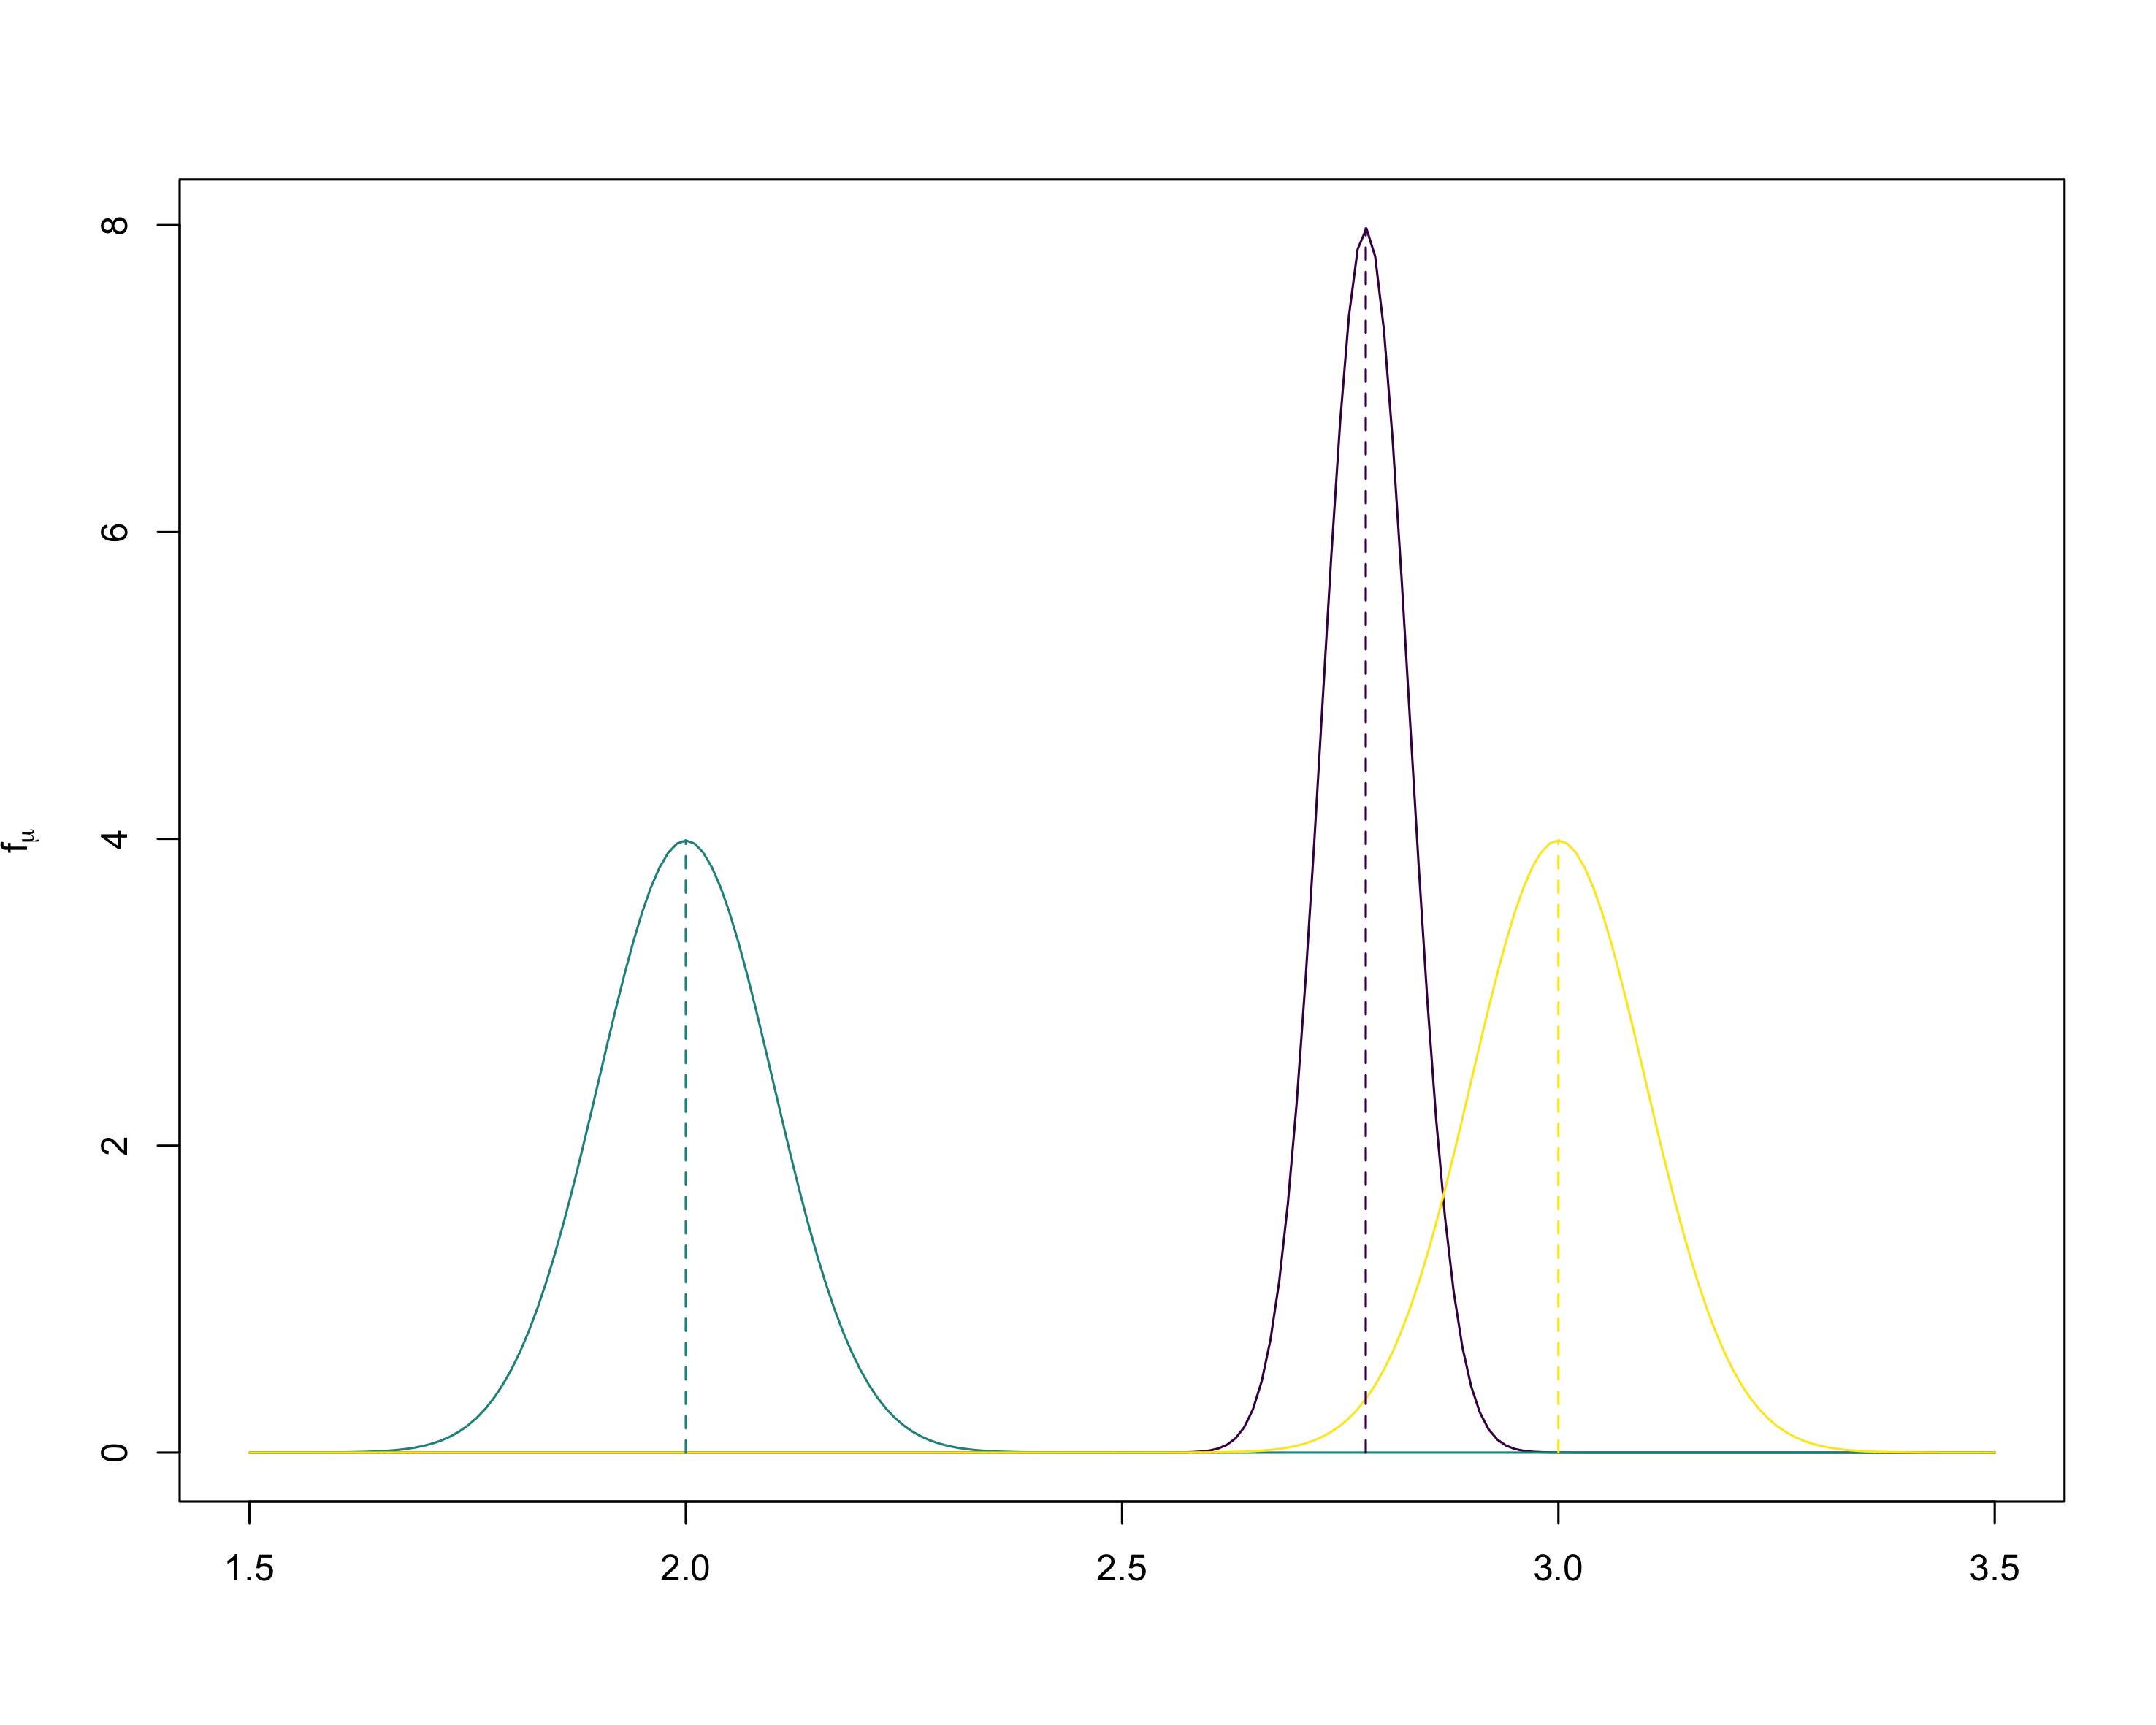
\includegraphics[width=12cm]{pointwise_estimation.png}
\caption{Funciones de distribución a priori (azul) y a posteriori (morado) para $\mu$ con los estimadores $m$ y $m_x$, junto con la función de verosimilitud (amarillo) y el verdadero valor $\mu = 3$.}
\label{fig:pointwise}
\end{figure}

Quien desee leer más sobre las bases teóricas de la estadística bayesiana se puede dirigir a \citet{bernardo} y \citet{mendoza}. Para un enfoque más aplicado se recomiendan \citet{gelman}, \citet{kruschke} y \citet{albert}. Para leer más sobre la historia de la estadística bayesiana y sus principales exponentes se recomienda \citet{bertsch}.

\newpage
\clearpage

\section{Métodos de simulación}
\label{simulacion}

La posibilidad de simular observaciones de variables aleatorias ha sido fundamental en el desarrollo de la estadística aplicada, ya que permite hacer estimaciones empíricas de cálculos que son muy complicados o incluso imposibles de resolver analíticamente. La simulación de variables aleatorias depende a su vez de poder simular observaciones de una distribución uniforme en $(0, 1)$ (ver \citet{dagpunar}). Este capítulo habla de cómo simular observaciones directamente con el método de la transformación inversa e indirectamente con métodos de aceptación y rechazo. Además se habla de técnicas de Monte Carlo para aproximar momentos de variables aleatorias y el uso de procesos estocásticos para simular virtualmente cualquier distribución con técnicas de Monte Carlo vía cadenas de Markov.

\subsection{Método de la transformada inversa}
\label{sec:transformada}

La función de distribución $F$ de una variable aleatoria $X$, definida como
\begin{align*}
F: \mathbb{R}&\to [0,1]\\
F(x) &= P\left(X \leq x\right)
\end{align*}
tiene las características siguientes:

\begin{enumerate}
\item $F$ es no decreciente,
\item $F$ es continua por la derecha,
\item $\lim\limits_{x\to +\infty}F(x) = 1$ y $\lim\limits_{x\to -\infty}F(x) = 0$.
\end{enumerate}
Se define la inversa generalizada de $F$, denotada $F^{-1}:[0,1]\to \mathbb{R}$, como $$F^{-1}(y) = \inf \{x\in \Omega_X: F(x) \geq y\}.$$ Con esta definición se puede verificar que
\begin{itemize}
\item $F^{-1}(F(x)) \leq x$ porque $F$ es no decreciente,
\item $F(F^{-1}(y)) \geq y$ por la definición de $F^{-1}$ y
\item $F^{-1}$ es no decreciente.
\end{itemize}
Más aún, si $F$ es estrictamente creciente se tiene que $F^{-1}(F(x)) = x$ y si $F$ es continua se cumple $F(F^{-1}(y)) = y$, por lo que $F^{-1}$ define la inversa de $F$ en el sentido usual si $F$ es continua y monótona estricta.

\begin{theorem}[Método de la transformación inversa] \label{teo:trans}
Sea $F$ una función de distribución, $F^{-1}$ su inversa generalizada y sea $U\sim U(0,1)$. Entonces la variable aleatoria $X$ definida como $X = F^{-1}(U)$ tiene función de distribución $F$.
\end{theorem}
\begin{proof}
Sea $x\in \mathbb{R}$ fija. Se quiere probar la contención de los eventos $$\{U<F(x)\}\subseteq\{F^{-1}(U)\leq x\}\subseteq\{U\leq F(x)\}.$$ Sea $u$ una observación de la variable aleatoria $U$.
$$u<F(x) \implies F^{-1}(u) \leq F^{-1}(F(x)) \leq x$$
$\therefore \hspace{2pt} \{U<F(x)\} \subseteq\{F^{-1}(U)\leq x\}$ y
$$F^{-1}(u)\leq x \implies u\leq F(F^{-1}(u))\leq F(x)$$
$\therefore \hspace{2pt} \{F^{-1}(U)\leq x\}\subseteq \{U \leq F(x)\}$.

De esta forma, se tiene que 
\begin{align*}
P\left(U\leq F(x)\right) = P\left(U<F(x)\right) &\leq P\left(F^{-1}(U)\leq x\right) \leq P\left(U \leq F(x)\right)\\
\implies F(x) = P\left(U \leq F(x)\right) &= P\left(F^{-1}(U)\leq x\right) = P\left(X\leq x\right)\\
\implies P\left(X \leq x\right) &= F(x),
\end{align*}
con lo que se concluye que $F$ es la función de distribución de $X$.
\end{proof}

Utilizando el teorema \ref{teo:trans}, se puede crear un algoritmo para simular observaciones de una variable aleatoria $X$ con función de distribución $F$:
\begin{enumerate}
\item Calcular $F^{-1}$, la inversa generalizada de $F$.
\item Simular observaciones de $U\sim U(0,1)$.
\item Evaluar $X=F^{-1}(U)$.
\end{enumerate}

Para ilustrar el algoritmo se utiliza como ejemplo la distribución exponencial. $X\sim Exp(\lambda)$ tiene función de densidad dada por $$f(x) = \lambda e^{-\lambda x} \mathbb{I}_{(0,\infty)}(x)$$ y función de distribución dada por $$F(x) = 1-e^{-\lambda x}\mathbb{I}_{[0,\infty)}(x).$$ Esta función de distribución es continua y estrictamente creciente en $\Omega_X=[0, \infty)$, por lo que su inversa generalizada corresponde a la inversa en el sentido usual. La inversa de $F$ es $$F^{-1}(y) = -\frac{1}{\lambda}\log (1-y)$$ con $Dom(F^{-1}) = [0, 1)$. En el cuadro \ref{cod:transformada_inversa} se muestra el código en R para la simulación de $X \sim Exp(\lambda = 1/2)$, junto con el histograma obtenido y la función de densidad en la figura \ref{fig:transformada_inversa}.

\begin{table}[htb]
\begin{lstlisting}
f <- function(x, lambda) lambda * exp(-lambda * x)
dist_inv <- function(y, lambda) -(1/lambda) * log(1-y)

set.seed(42)
nsim <- 10e4
lambda <- 0.5

u <- runif(nsim)
x <- dist_inv(u, lambda)
\end{lstlisting}
\caption{Código para simular observaciones de $X \sim Exp(\lambda = 0.5)$ en R.}
\label{cod:transformada_inversa}
\end{table}

\begin{figure}[htb]
\centering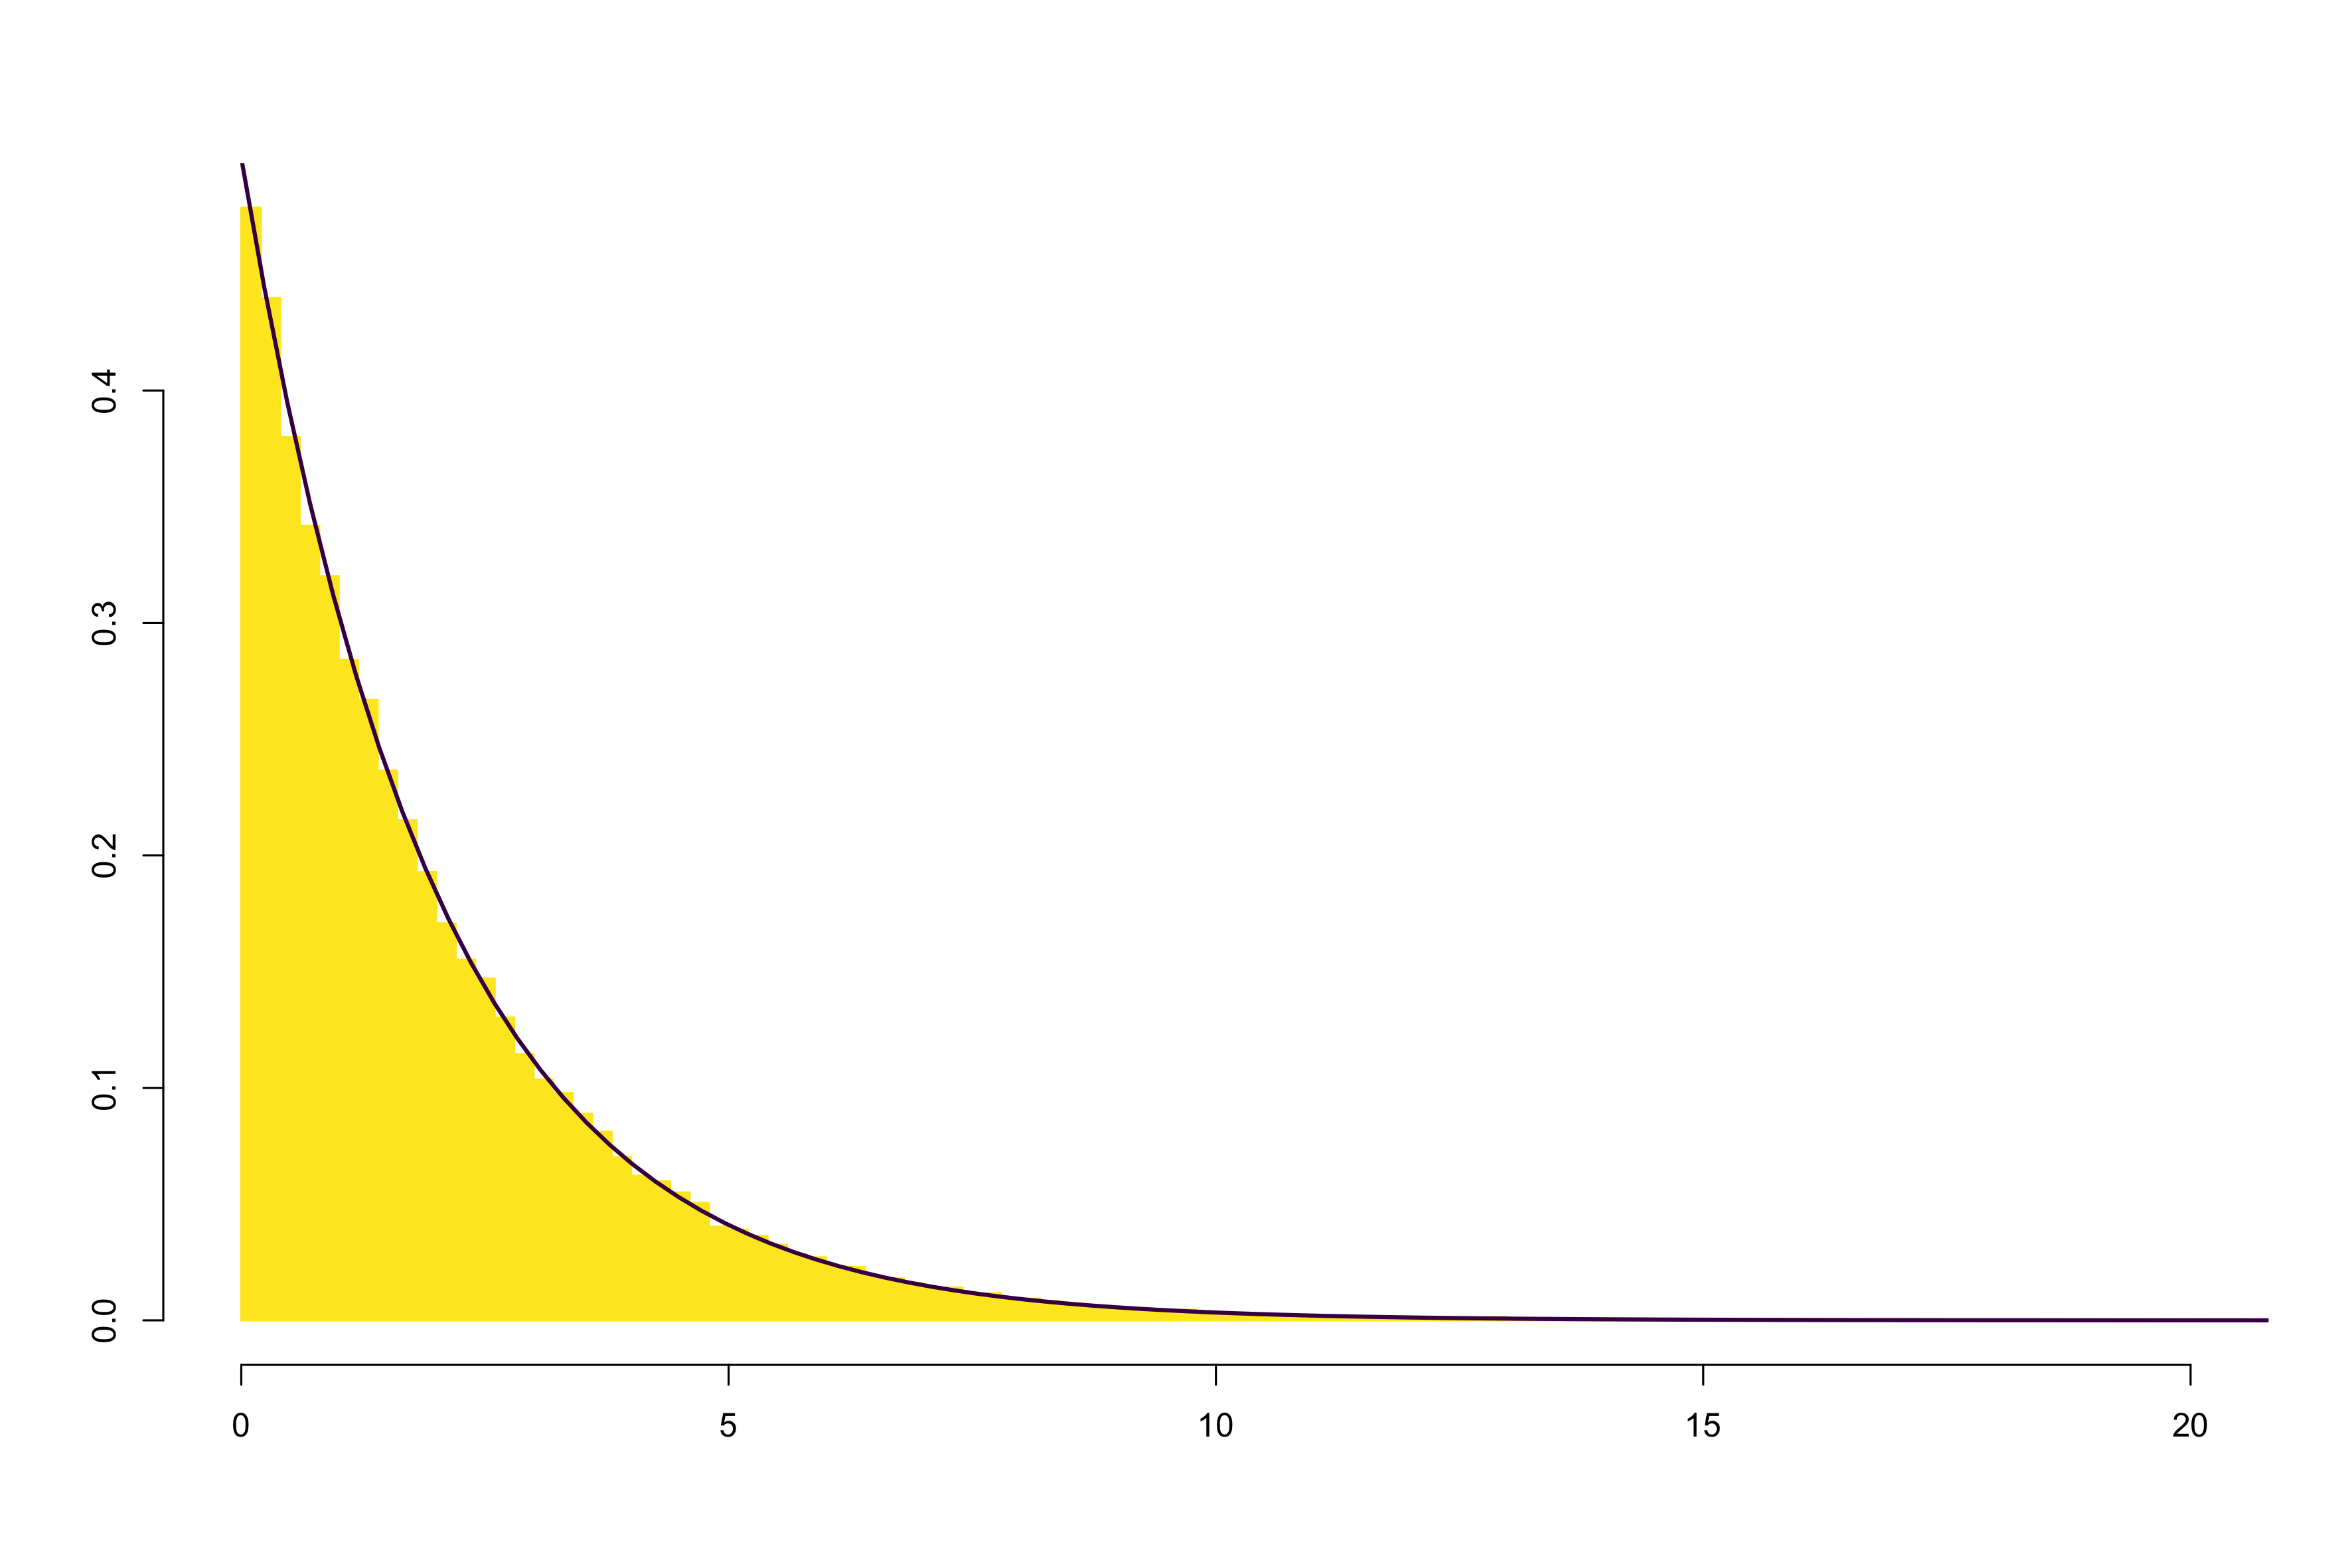
\includegraphics[width=10cm]{transformada_inversa.png}
\caption{Histograma de las simulaciones de $X \sim Exp(0.5)$ con la densidad real.}
\label{fig:transformada_inversa}
\end{figure}

\newpage

\subsubsection*{Simular distribuciones representadas como mezclas.} Supóngase que una variable aleatoria $X$ puede ser representada como una mezcla, esto es
\begin{equation}
f(x) = \int_{\Omega_Y} f(x|y)g(y)dy.
\label{mezcla_sim}
\end{equation}
Idealmente, $g(y)$ y $f(x|y)$ deben ser densidades fáciles de simular, por ejemplo, con el método de la transformada inversa. Para simular entonces observaciones de $X$ se utiliza el algoritmo siguiente \citep{casella}:

\begin{enumerate}
\item Simular una observación $y$ de $Y\sim g$.
\item Simular $X|y \sim f(x|y)$.
\item Las observaciones resultantes tienen una distribución dada por la función de densidad \eqref{mezcla_sim}.
\end{enumerate}

Las librerías de R base no cuentan con una función para simular directamente la distribución $t$ con parámetros de localización y escala. Se aprovecha su representación como mezcla para crear un algoritmo que permita simularla. En \citet{gelman} se menciona que si $X\sim t_\nu (\mu, \sigma^2)$, entonces $X$ puede ser representada como una mezcla tomando 
\begin{align*}
X|Y &\sim \mathcal{N}(\mu , Y)\\
Y &\sim \chi ^{-2}(\nu, \sigma ^2),
\end{align*}
donde $\chi ^{-2}(\nu, \sigma ^2)$ se refiere a una distribución ji-cuadrada inversa y escalada con parámetro de escala $\sigma^2$ y $\nu$ grados de libertad, o de manera equivalente
\begin{align*}
X|Y &\sim \mathcal{N}(\mu , Y)\\
\frac{\nu\sigma ^2}{Y} &\sim \chi ^2_{\nu}.
\end{align*}

Las observaciones de la distribución Normal se obtienen con la función \texttt{rnorm}. La documentación de esta función, accesible con el comando \texttt{?rnorm} indica que esta simulación se hace utilizando el método de la transformada inversa. La simulación de la distribución $\chi^2$ se hace utilizando la función \texttt{rchisq} en R. En la documentación de esta función se puede leer que las observaciones se obtienen simulando una distribución Gamma, la cual se simula con un método de aceptación y rechazo como los que se presentan en la sección \ref{aceptacion}. El histograma y la densidad real se muestran en la figura \ref{fig:t}.

\begin{figure}[!htb]
\centering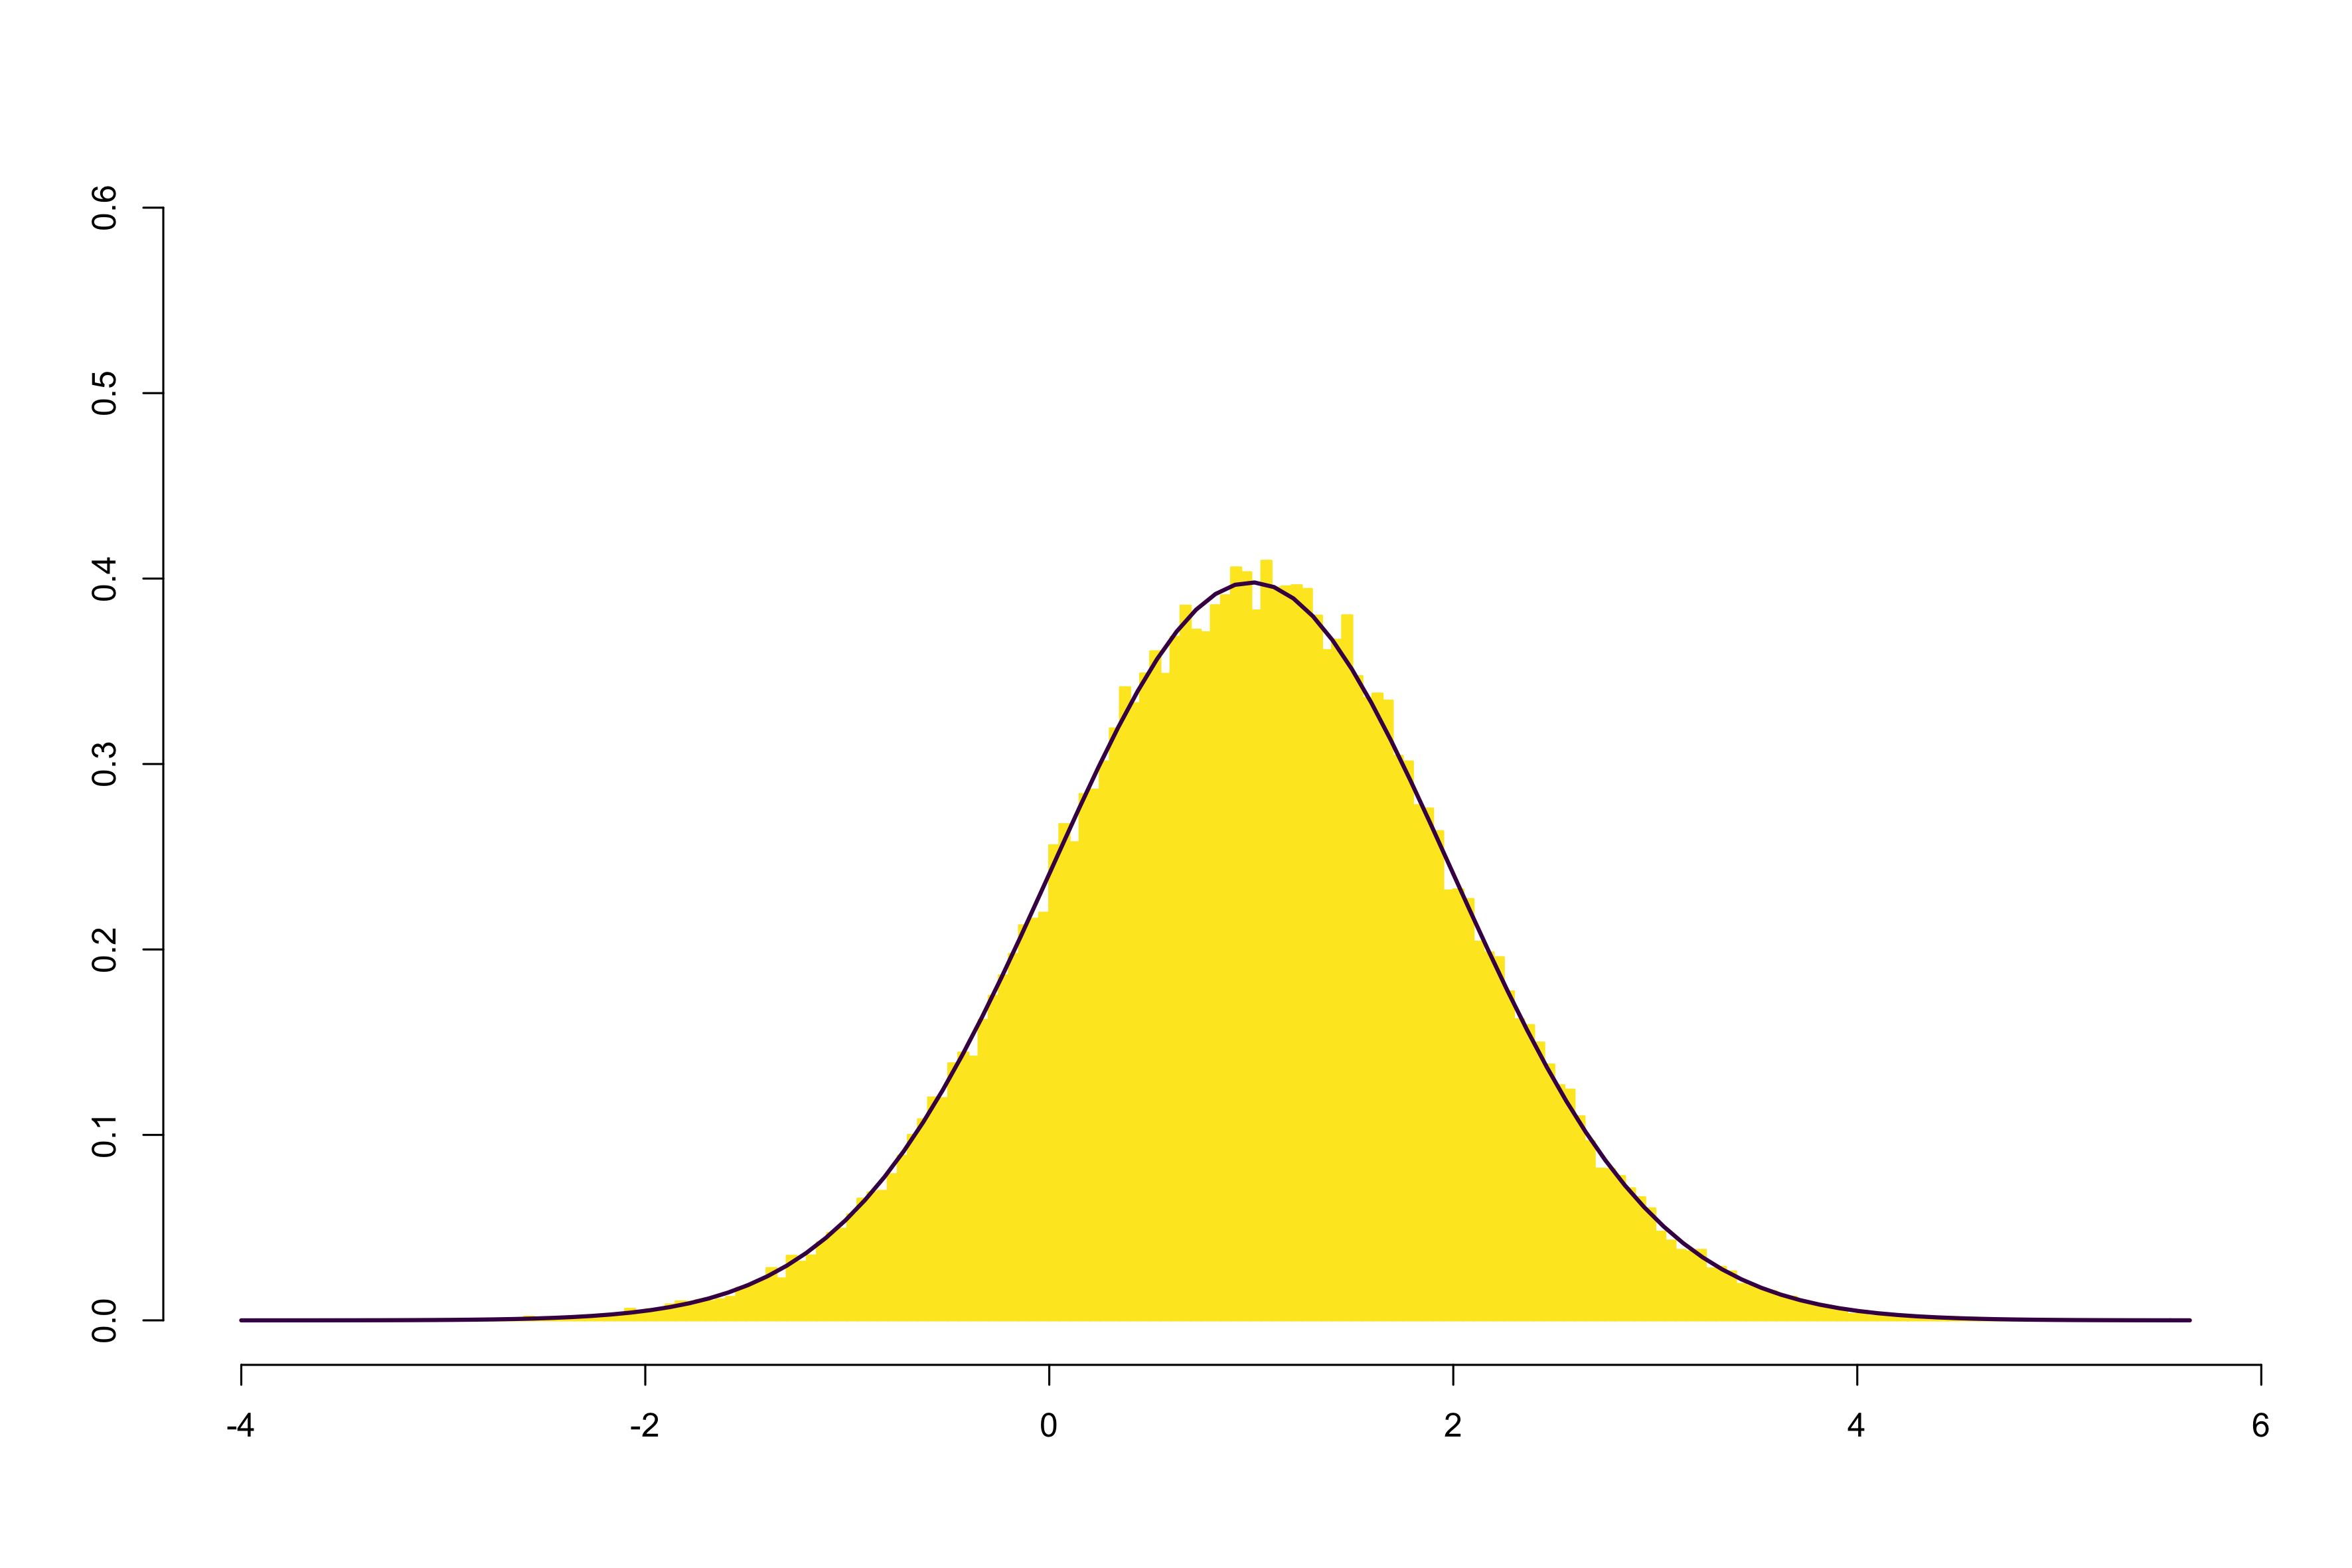
\includegraphics[width=10cm]{sim_mezcla.png}
\caption{Histograma de las simulaciones de $X \sim t_{(100)} (\mu = 1, \sigma^2 = 1)$ con la densidad real.}
\label{fig:t}
\end{figure}

Otro ejemplo de distribuciones generadas por mezclas es el de la distribución Poisson-gamma, denotada $Pg(\alpha, \beta, \gamma)$. Se presenta este ejemplo porque la distribución es utilizada en la sección \ref{elmodelo}. La función de probabilidad de una variable aleatoria discreta $X$ con distribución Poisson-gamma está dada por
\begin{equation}
\label{eq:poga}
p(x | \alpha, \beta, \gamma) = \frac{\beta ^ \alpha}{\Gamma (\alpha)}\frac{\Gamma (\alpha + x)}{x!}\frac{\gamma ^ x}{(\beta + \gamma) ^ {\alpha + x}}
\end{equation}
con $\Omega_X = \mathbb{N} \cup \lbrace 0 \rbrace$ y $\alpha, \beta, \gamma \in \mathbb{R}^+$. En \citet{bernardo} se menciona que esta distribución es generada por una mezcla de la forma
$$p(x | \alpha, \beta, \gamma) = \int_0 ^\infty Po(x | \gamma \lambda) Ga(\lambda | \alpha, \beta) \ d\lambda,$$ donde $Ga(\alpha, \beta)$ se refiere a la distribución gamma con valor esperado $\alpha / \beta$. Se puede utilizar el algoritmo anterior para simular observaciones de \eqref{eq:poga}. En la figura \ref{fig:poga} se presenta el histograma de las simulaciones para $\alpha = 2$, $\beta = 1$ y $\gamma = 5$. Para simular las observaciones de $Ga(\lambda | \alpha, \beta)$ y $Po(x | \gamma \lambda)$ se utilizan las funciones \texttt{rgamma} y \texttt{rpois} incluidas en los paquetes de R base.

\begin{figure}[htb]
\centering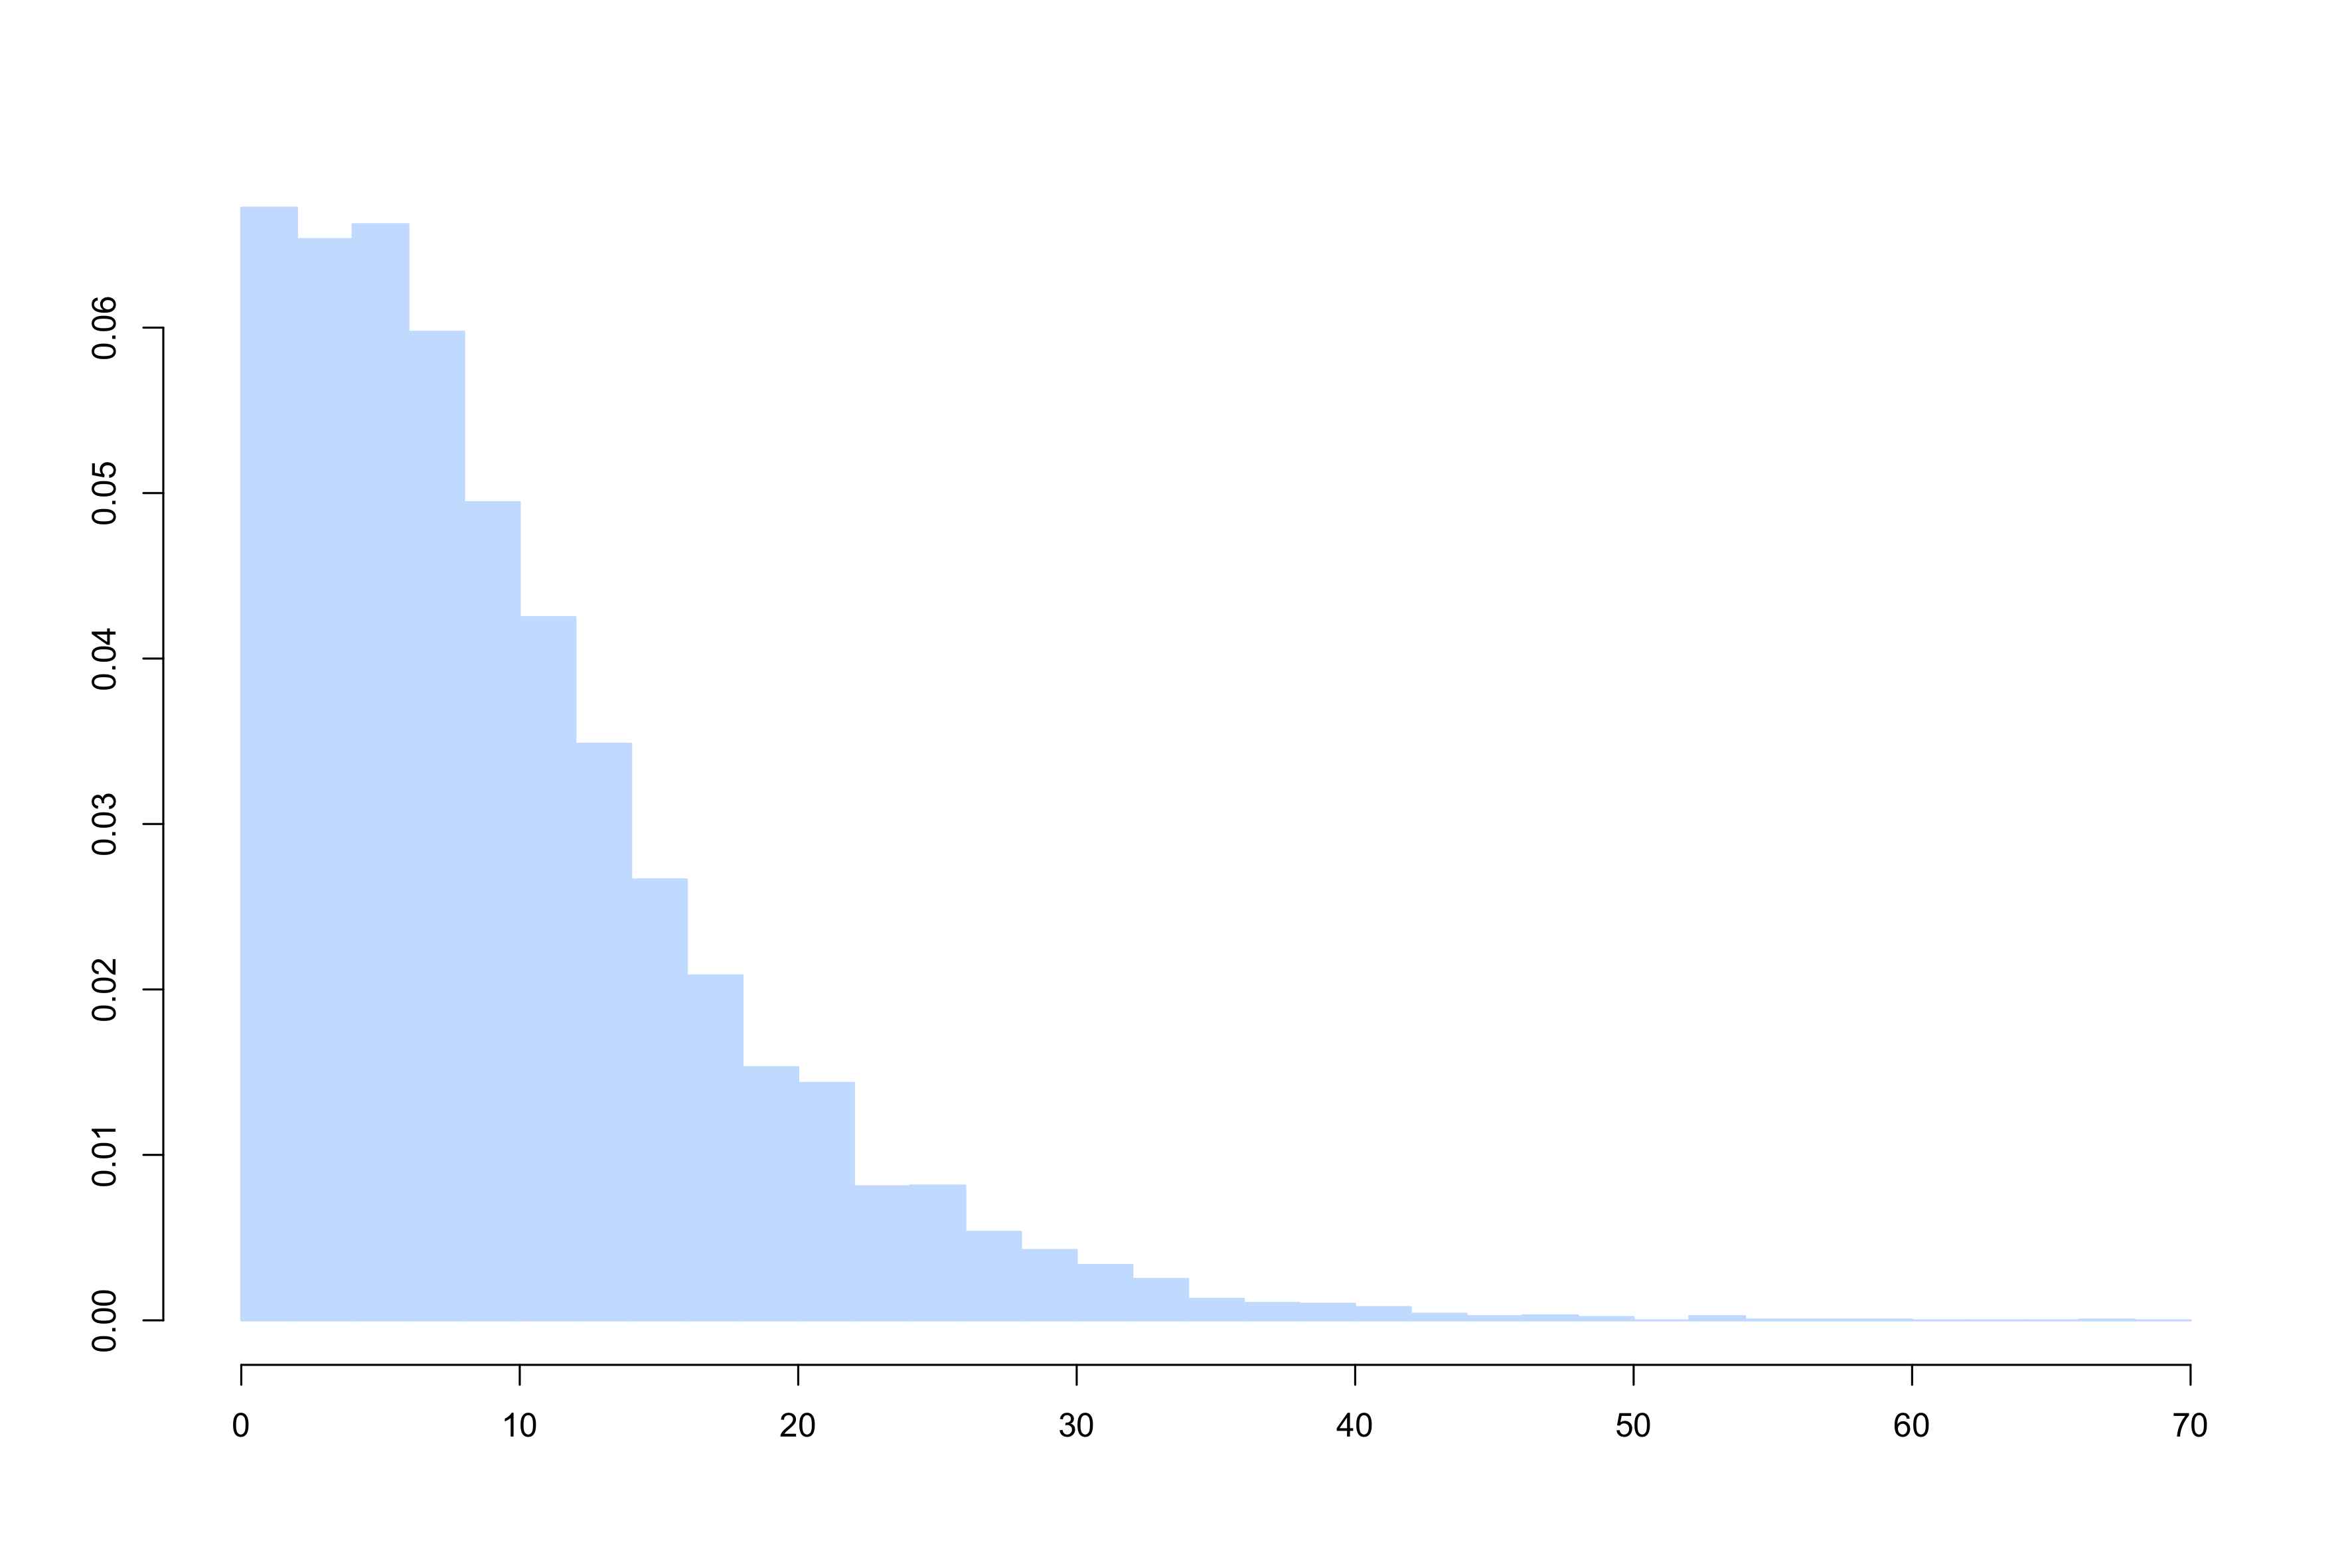
\includegraphics[width=10cm]{poisson_gamma.png}
\caption{Histograma de las simulaciones de $X \sim Pg(2, 1, 5)$.}
\label{fig:poga}
\end{figure}

\newpage

Es común en inferencia estadística bayesiana que las distribuciones posteriores de las cuales se quieren obtener muestras sean conocidas salvo por una constante. En estos casos, el método de la transformada inversa no se puede utilizar ya que no podemos obtener la inversa generalizada $F^{-1}$. Sin embargo, si la distribución de interés es discreta, existe una manera sencilla de aproximar esta constante. A continuación, se presenta un ejemplo para ilustrar esta técnica utilizada en la sección \ref{elmodelo} para obtener muestras de este tipo.

Sea $X$ una variable aleatoria con distribución Poisson, $X \sim Po(\lambda),$ $\lambda > 0$. La función de probabilidad de $X$ está dada por
$$P(X = x) = \frac{\lambda ^ x}{x!}e^{-\lambda}$$ con $\Omega_X = \lbrace 0, 1, 2, \dots \rbrace$. Supóngase ahora que no se conoce la constante $e^{-\lambda}$ y que únicamente se sabe que $$P(X = x) \propto  \frac{\lambda ^ x}{x!}.$$ Como $$\sum_{x \in \Omega_X} P(X = x) = 1,$$ se sigue que $$\sum_{x \in \Omega_X} \frac{\lambda ^ x}{x!} = e^{\lambda}$$ y se tiene que la constante $$e^{-\lambda} = \left( \sum_{x \in \Omega_X} \frac{\lambda ^ x}{x!}\right) ^{-1}.$$ Si se desean obtener muestras de $X$, se puede fijar un límite $\Lambda >> 0$, donde el símbolo $>>$ denota ``mucho mayor'', y utilizar la aproximación $$ e^{\lambda} \approx \sum_{x = 0}^{\Lambda} \frac{\lambda ^ x}{x!}$$ para el método de la transformada inversa. En el cuadro \ref{cod:poisson} se presenta el código de R para obtener muestras de una variable aleatoria $X \sim Po(10)$ con esta técnica para $\Lambda = 65$ y se compara la función masa de probabilidad empírica con la ``verdadera'' dada por la función $\mathtt{dpois}$ en la figura \ref{fig:poisson}.

\begin{table}[htb]
\begin{lstlisting}
tol <- 10e-30
x <- 0
acum <- 0
lambda <- 10
prob <- 1
f <- c()

while(prob > tol) {
 densidad <- x * log(lambda) - lgamma(x + 1)
 densidad <- exp(densidad)
 acum <- acum + densidad
 prob <- densidad/acum
 f <- c(f, densidad)
 x <- x + 1
}

pois <- f / acum
muestra <- sample(1:x, size = 1e6, replace = TRUE, prob = pois)
\end{lstlisting}
\caption{Código para simular $X \sim Po(10)$ en R. }
\label{cod:poisson}
\end{table}

\begin{figure}[htb]
\centering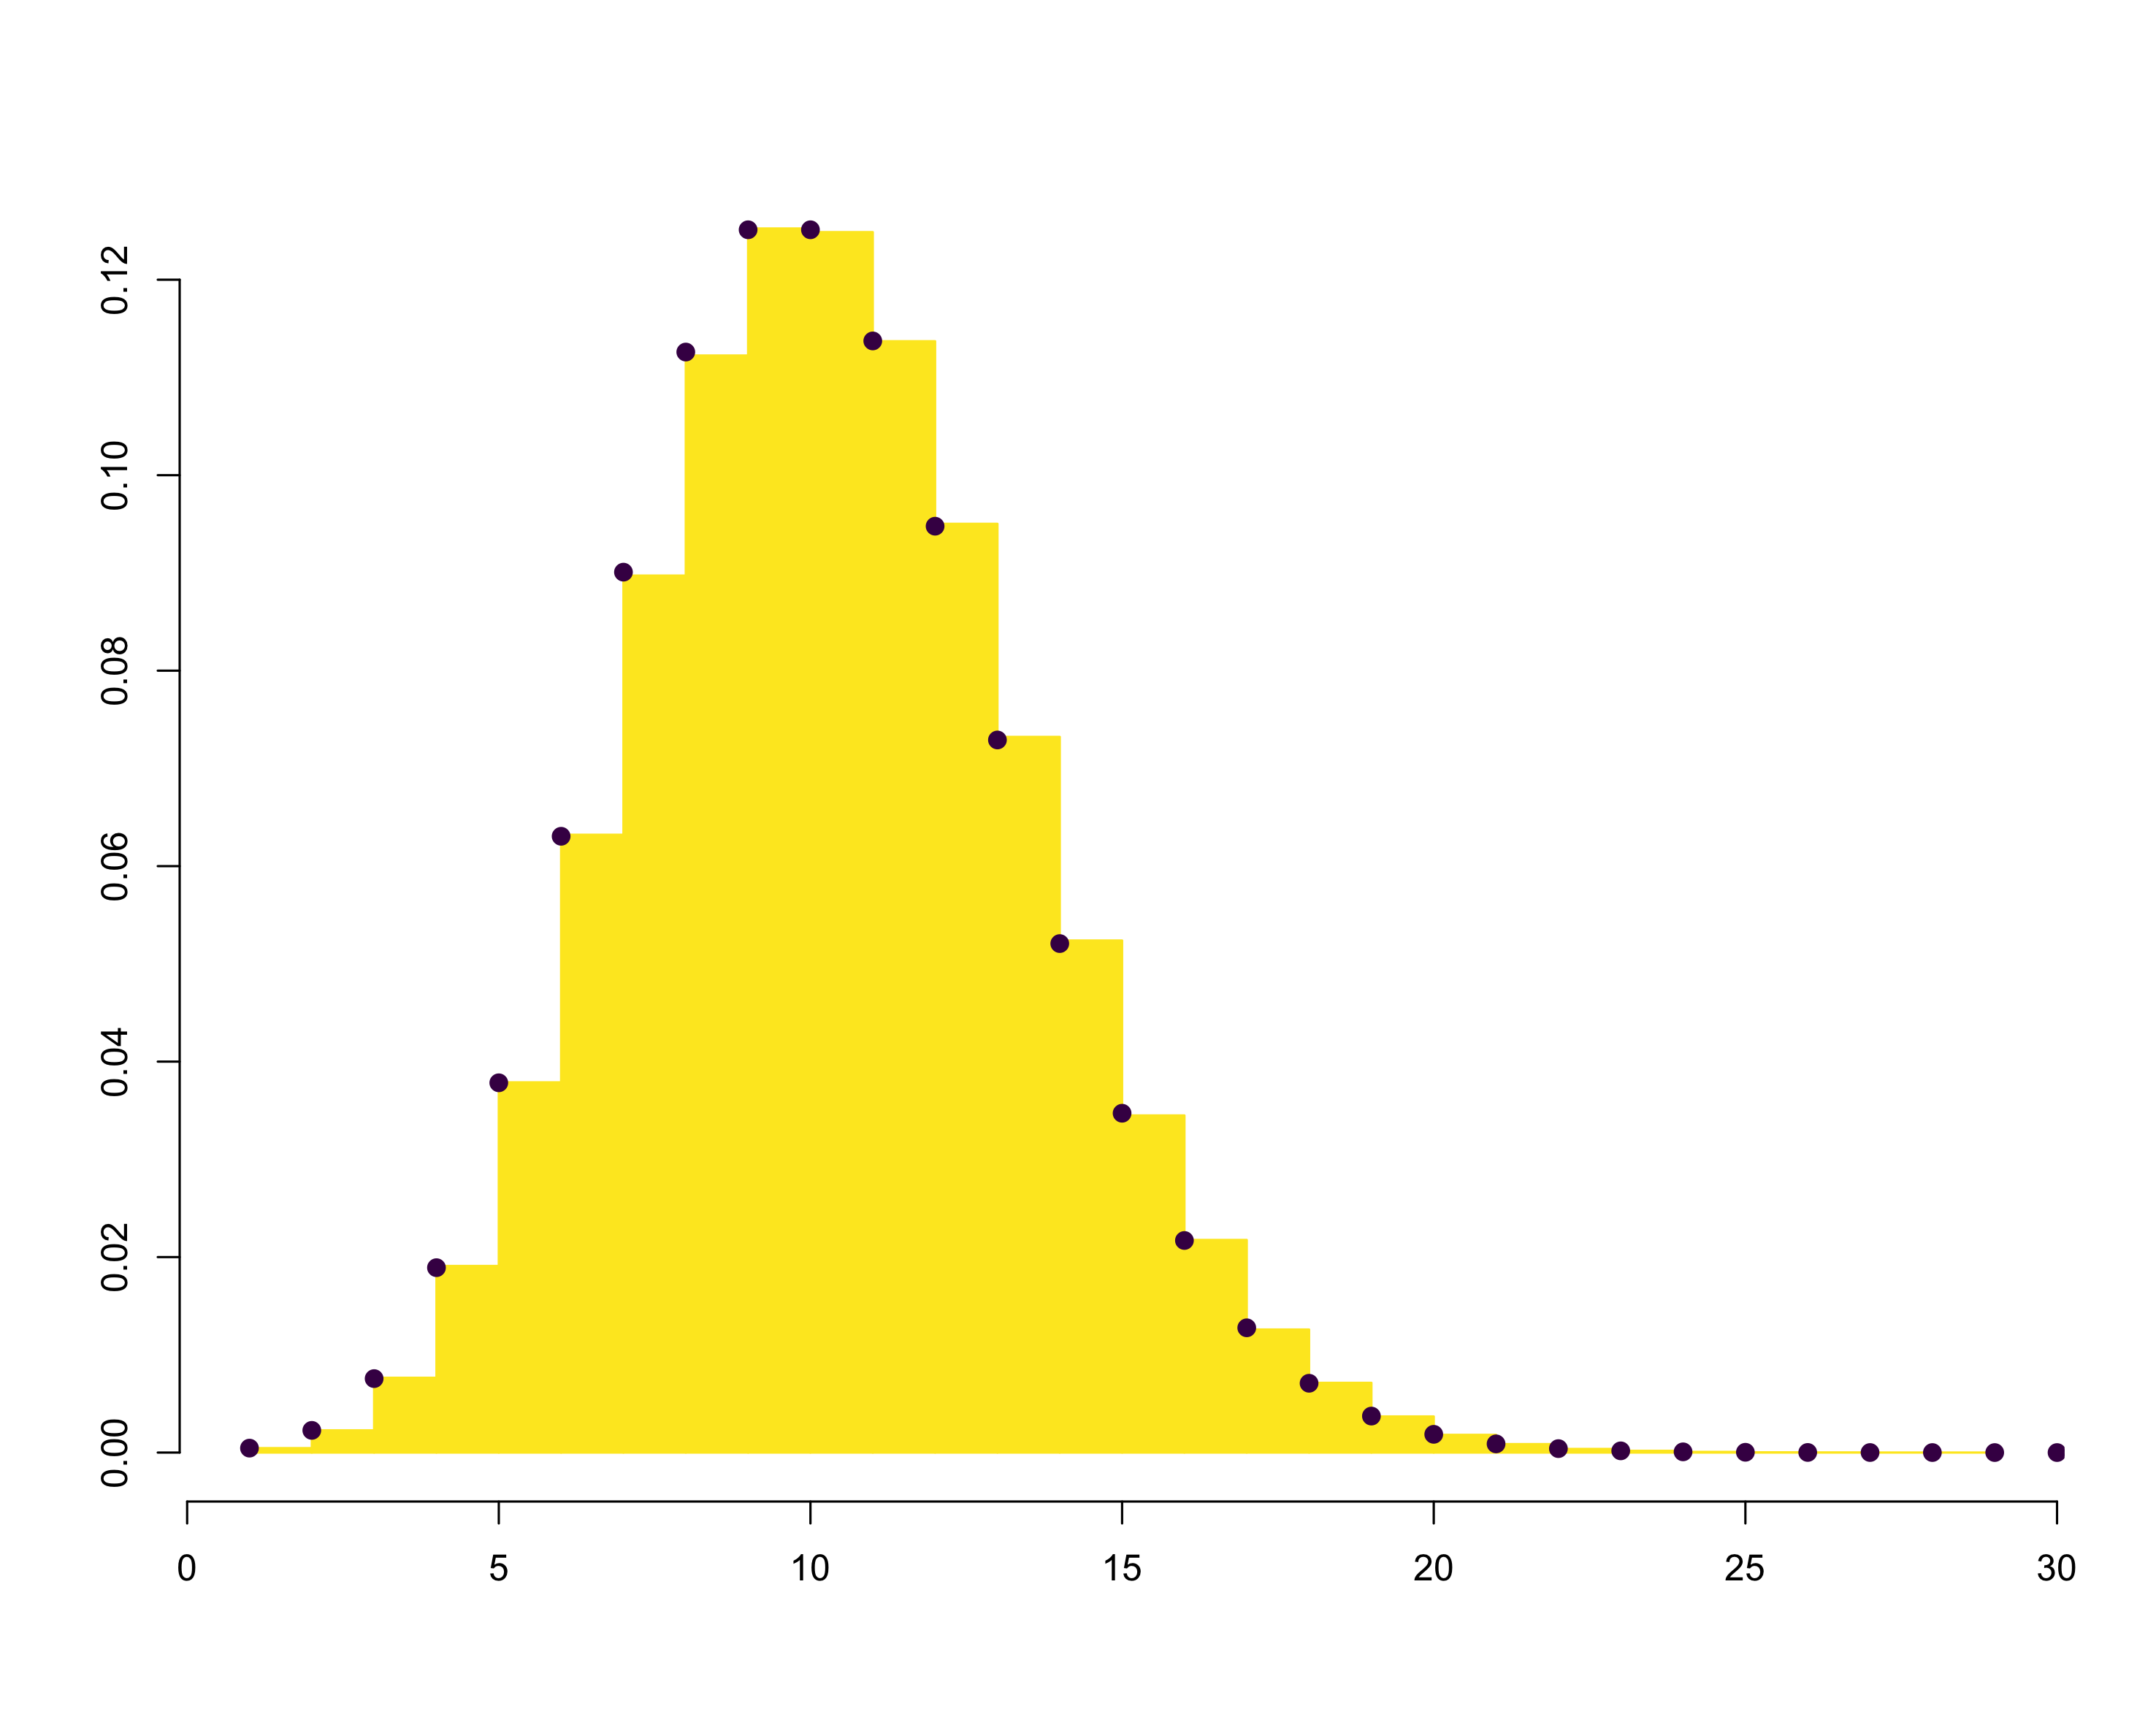
\includegraphics[width=10cm]{poisson.png}
\caption{Histograma de las simulaciones de $X \sim Po(10)$ con la masa de probabilidad real (puntos).}
\label{fig:poisson}
\end{figure}

\newpage

\subsection{Métodos de aceptación y rechazo}
\label{aceptacion}

Los métodos de aceptación y rechazo se utilizan cuando no se pueden obtener simulaciones de la distribución de interés por medio del método de la transformada inversa o con otras transformaciones de variables aleatorias. Si se quieren simular observaciones de una variable aleatoria $X$ con función de densidad $f$, se necesita una función de densidad $g$ tal que:
\begin{enumerate}
\item $\{x: f(x) > 0\}\subseteq \{x: g(x) > 0\}$.
\item $\exists M \in \mathbb{R}$ tal que $f/g \leq M.$
\end{enumerate}
A la densidad $f$ se le llama \textit{distribución objetivo} y a $g$ \textit{distribución candidata}. El algoritmo mencionado en \citet{casella} para simular observaciones de $X$ es:
\begin{enumerate}
\item Generar una observación $y$ de $Y\sim g$.
\item Generar una observación $u$ de $U\sim U(0,1)$ independiente de $Y$.
\item Si $u \leq \frac{1}{M}\frac{f(y)}{g(y)}$, aceptar $y$ como una observación de $X$.
\end{enumerate}

La siguiente proposición muestra por qué este algoritmo sirve para simular observaciones de $X \sim f$.

\begin{proposition}[Método de aceptación y rechazo] Sean $X\sim f$ y $Y \sim g$ dos variables aleatorias tales que $\Omega_X \subseteq \Omega_Y$ y $\exists M \in \mathbb{R}$ tal que $f(x)/g(x) \leq M$ $\forall x \in \Omega_X$. Sea $x \in \Omega_X$, entonces $$P\left( Y \leq x \  \vline \ U\leq \frac{1}{M}\frac{f(Y)}{g(Y)}\right) = P\left(X\leq x\right).$$
\end{proposition}
\begin{proof}
$$P\left( Y \leq x \  \vline \ U\leq \frac{1}{M}\frac{f(Y)}{g(Y)}\right) = \frac{P\left( Y\leq x, \ U \leq \frac{f(Y)}{Mg(Y)}\right)}{P\left( U \leq \frac{f(Y)}{Mg(Y)}\right)}.$$ Para el denominador se tiene 
\begin{align*}
P\left( U \leq \frac{f(Y)}{Mg(Y)}\right) &= \int_{\Omega_Y}P\left( U \leq \frac{1}{M}\frac{f(y)}{g(y)} \ \vline \ Y=y\right) g(y) dy\\
&= \int_{\Omega_Y}\int_0^{M^{-1} f(y)/g(y)} g(y)du \ dy\\
&= \int_{\Omega_Y}g(y)\left(\int_0^{M^{-1} f(y)/g(y)} du\right)\ dy\\
&= \int_{\Omega_Y}\frac{1}{M}f(y) \ dy\\
&= \frac{1}{M}
\end{align*}
y para el numerador se tiene
\begin{align*}
P\left( Y \leq x, \ U \leq \frac{1}{M}\frac{f(Y)}{g(Y)}\right) &= \int_{-\infty}^x\int_0^{M^{-1} f(y)/g(y)} du \ g(y) \ dy\\
&= \int_{-\infty}^x \frac{f(y)}{M} \ dy\\
&= \frac{1}{M} F(x).
\end{align*}
Por lo tanto, se tiene que $$P\left( Y \leq x \  \vline \ U\leq \frac{1}{M}\frac{f(Y)}{g(Y)}\right) = F(x) = P\left(X \leq x\right).$$
Al seguir esta demostración, nótese que el algoritmo no depende de las constantes de normalización, por lo que se pueden utilizar funciones proporcionales a $f$ y $g$ para las que se conozca la constante $M$.
\end{proof}

Encontrar una cota $M$ para el cociente $f/g$ implica que se cuenta con una infinidad de cotas para este cociente. En la demostración anterior se prueba que $P\left( U \leq \frac{1}{M}\frac{f(Y)}{g(Y)}\right) = 1/M$, es decir, la probabilidad de aceptación en el algoritmo es de $1/M$. Este hecho muestra la importancia de elegir la constante $M$ tan pequeña como sea posible, ya que una baja probabilidad de aceptación puede resultar en un algoritmo costoso e ineficiente en términos computacionales. En teoría, sería útil generar un algoritmo para optimizar la constante $M$ y que tenga el menor valor posible. Sin embargo, en la práctica se debe tomar en cuenta el uso que se va a hacer del algoritmo de aceptación y rechazo. Por ejemplo, si solamente se necesita generar una muestra aleatoria, el costo de optimizar $M$ puede ser mucho mayor a la pérdida de eficiencia por utilizar una $M$ más grande.

Ahora se presenta un ejemplo del método de aceptación y rechazo para obtener muestras de una distribución $Ga(2, 1)$. Como distribución candidata se utiliza $g \sim Exp(0.5).$ El histograma de las simulaciones se encuentra en la figura \ref{fig:acep_rech} y el código en el cuadro \ref{cod:acep_rech}. Se utilizó el valor $M = 4/e \approx 1.47$ con el cual se tiene que alrededor del 68 \% de las simulaciones son aceptadas.

\begin{table}[!htb]
\begin{lstlisting}
f <- function(x) {dgamma(x, shape = 2, rate = 1)}
g <- function(x) {dexp(x, rate = 0.5)}
h <- function(x) {f(x)/g(x)}

set.seed(42)
n.sim <- 1e5
M <- 4/exp(1)

proposal <- rexp(n = n.sim, rate = 0.5)
u <- runif(n = n.sim)
aceptados <- u <= 1/M * h(proposal)

sample.f <- proposal[aceptados]
\end{lstlisting}
\caption{Código para generar las simulaciones de $Ga(2, 1)$ en R. }
\label{cod:acep_rech}
\end{table}

\begin{figure}[!htb]
\centering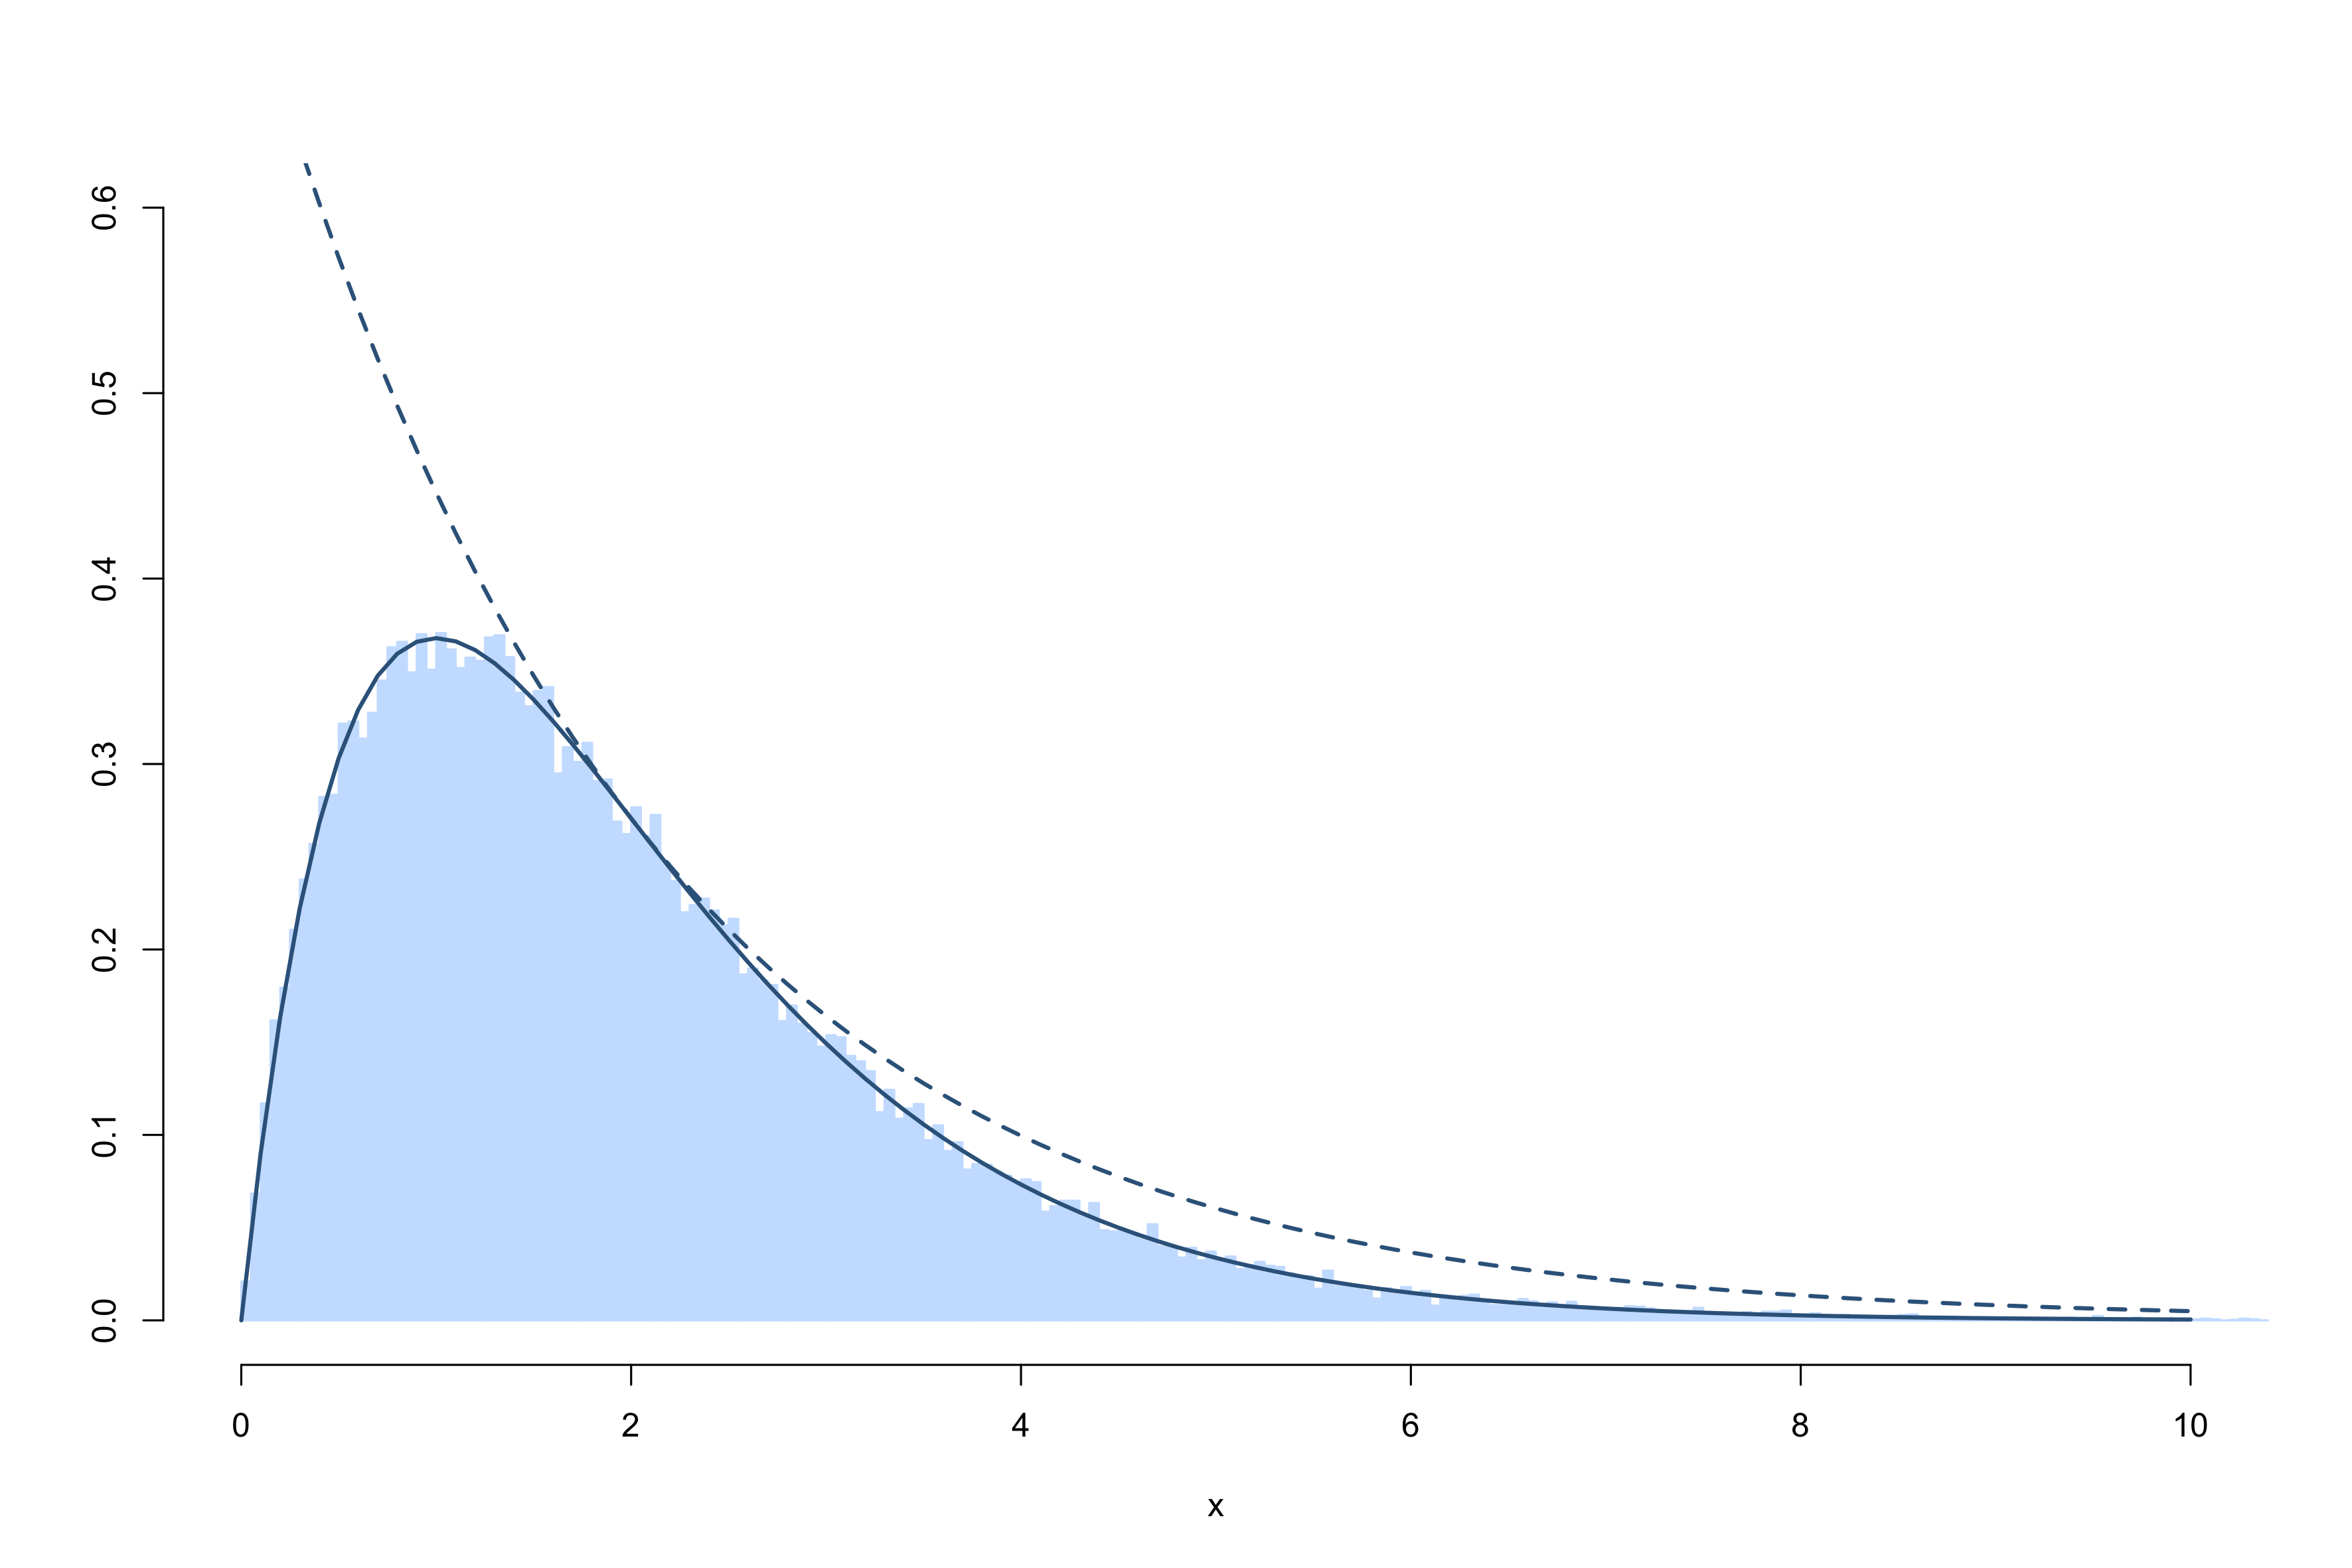
\includegraphics[width=10cm]{aceptacion_rechazo.png}
\caption{Histograma de las simulaciones de $Ga(2, 1)$, con la densidad real $g(x)$ (línea continua) y la curva $M f(x)$ (línea punteada).}
\label{fig:acep_rech}
\end{figure}

\newpage

Es importante resaltar que es preferible utilizar el método de la transformación inversa cuando sea posible, ya que cada observación generada por medio de ese método es utilizada como observación de $F$. Por el contrario, en los métodos de aceptación y rechazo se generan observaciones ``basura" (rechazadas) que no son utilizadas, por lo que se necesitan más iteraciones para obtener una muestra de tamaño $n$. En R es recomendable utilizar cuando sea posible alguna de las funciones ya implementadas para simular variables aleatorias como $\mathtt{rnorm}$, $\mathtt{runif}$, $\mathtt{rgamma}$, etc., ya que están optimizadas para minimizar el tiempo de las simulaciones y se puede consultar su documentación con el comando $\mathtt{help()}$ o `$\mathtt{?}$'.

Los algoritmos presentados en las secciones \ref{sec:transformada} y \ref{aceptacion} son la base de la simulación de variables aleatorias. Con ellos, se pueden generar muestras de una gran cantidad de distribuciones. Además, si se tienen los medios para generar observaciones de una variable aleatoria $X$, entonces se pueden generar directamente observaciones de cualquier transformación de esta variable aleatoria que tenga la forma $Y = g(X)$, simplemente evaluando la función $g$ en cada observación simulada de $X$.

\subsection{Monte Carlo vía cadenas de Markov}	
\label{sec_cadenas}
\epigraph{\itshape The combination of Bayes and MCMC has been called ``arguably the most powerful mechanism ever created for processing data and knowledge".}{---Sharon B. McGrayne, \textit{The Theory That Would Not Die.}}
\subsubsection*{Integración Monte Carlo}

Se conoce como integrácion Monte Carlo a un conjunto de técnicas utilizadas para aproximar integrales. La principal característica de estas técnicas es que se basan en algoritmos de simulación para realizar las aproximaciones a través de muestras aleatorias \citep{casella}. Su funcionamiento es consecuencia de uno de los resultados más famosos de la teoría de probabilidad, la \textit{ley fuerte de los grandes números} (ver \citet{feller}).

Las técnicas de integración Monte Carlo buscan aproximar integrales de la forma
$$\theta = E[h(x)] = \int_{\Omega_X} h(x) \ dF(x),$$ donde $F$ es la función de distribución de una variable aleatoria $X$ y $\Omega_X$ su soporte. Como consecuencia del teorema \ref{grandes_numeros}, para estimar $\theta$ se simula una muestra aleatoria $X_1, X_2, \dots, X_n$ con $X_i\sim F$ y se utiliza el estimador $$\hat{\theta} = \frac{1}{n}\sum_{i=1}^n h(x_i).$$ Esto significa que se pueden explotar las técnicas de las secciones \ref{sec:transformada} y \ref{aceptacion} para realizar estas estimaciones.

Como ejemplo supóngase que se quiere estimar la integral
\begin{equation}\label{eq:integral}
\theta = \int_0^2 x^4 \ dx.
\end{equation}
Esta integral se puede resolver analíticamente y se obtiene el valor $\theta = 6.4$, sin embargo se utiliza aquí para entender los conceptos y evaluar el error de aproximación. Se puede reescribir a $\theta$ como $$\theta = 2E[X^4] =  2\int_0^2 x^4 \ dF(x)$$ con $F(x) = U(0,2).$ Para aproximar a $\theta$ se realizan cien mil simulaciones de $X\sim U(0,2)$ y se obtiene el estimador $$\hat{\theta} = \frac{2}{100,000}\sum_{i=1}^{100,000} x_i^4 = 6.432671.$$ Este estimador tiene un error relativo de 0.051 \% respecto al verdadero valor $\theta = 6.4$. El código se presenta en el cuadro \ref{cod:integral}.

\begin{table}[htb]
\begin{lstlisting}
g <- function(x) x^4

nsim <- 10e4
set.seed(1996)

x <- runif(nsim, min = 0, max = 2)
theta_hat <- 2 * mean(g(x))
\end{lstlisting}
\caption{Código para aproximar la integral \eqref{eq:integral} con una muestra $U(0, 2)$ en R.}
\label{cod:integral}
\end{table}

Otro ejemplo de cómo utilizar muestras aleatorias para aproximar integrales se puede hacer utilizando la interpretación geométrica de la integral. Supóngase que se quiere estimar la misma cantidad $$\theta = \int_0^2 x^4 \ dx.$$ Geométricamente, esta integral es el área bajo la curva $h(x) = x^4$ para $0 \leq x \leq 2$. Viendo la figura \ref{fig:hx}, se puede ver que $\theta$ es una fracción del área del rectángulo $$\mathcal{R} = \left\lbrace (x, y) \in \mathbb{R}^2: 0\leq x \leq 2, \ 0 \leq y \leq 16\right\rbrace,$$ denotada $\Theta$. Se pueden simular puntos distribuidos de manera uniforme en $\mathcal{R}$. La probabilidad de que uno de estos puntos esté en el área $\Theta$ es $\theta / 32$, donde 32 es el área de $\mathcal{R}.$ Por lo tanto, se puede estimar a $\theta$ utilizando $$\hat{\theta} = \frac{\text{\# de puntos que caen en }\Theta}{\text{\# de puntos simulados}} \times 32$$ como se muestra en el cuadro \ref{cod:sim_hx}.

\begin{figure}[!htb]
\centering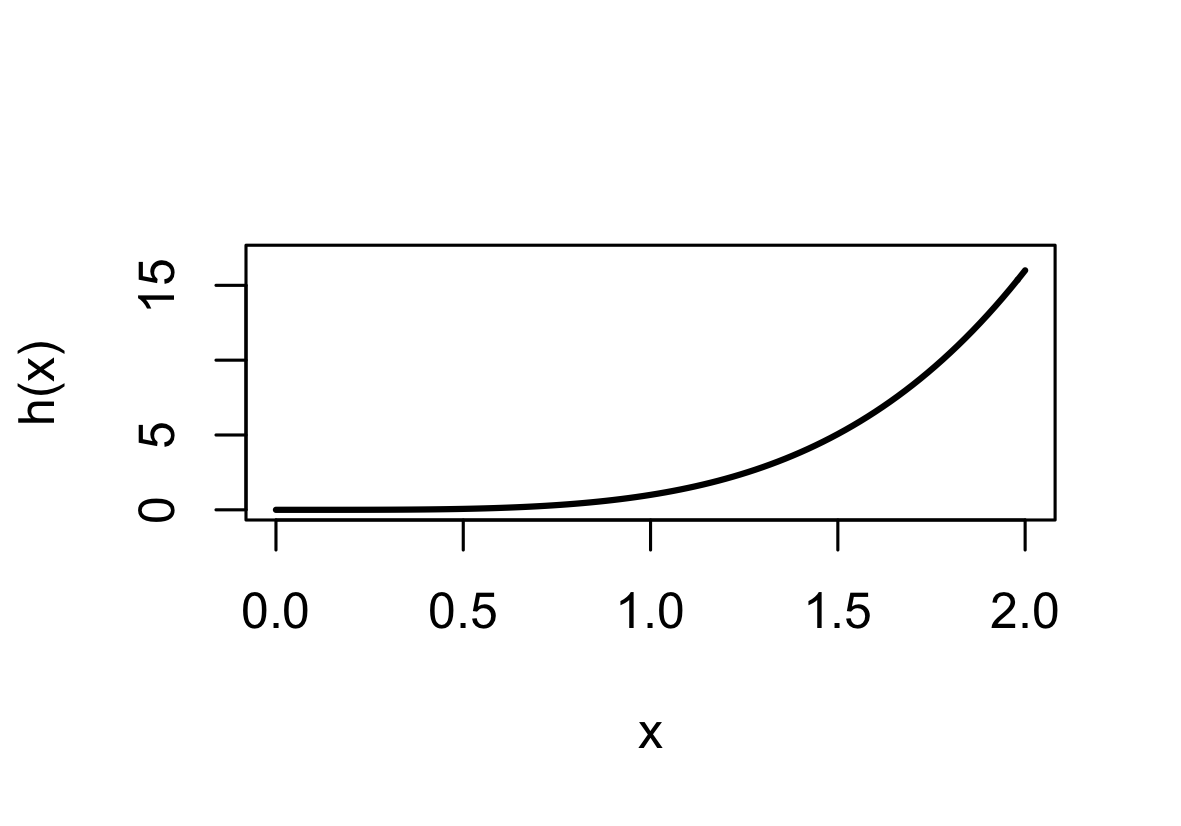
\includegraphics[width=10cm]{hx.png}
\caption{Gráfica de $h(x) = x^4$ para $x\in [0,2]$.}
\label{fig:hx}
\end{figure}

\begin{table}[!htb]
\begin{lstlisting}
y <- runif(nsim, min = 0, max = 16)

exito <- if_else(y <= g(x), 1, 0)

theta_hat2 <- mean(exito) * 32
\end{lstlisting}
\caption{Código para aproximar la integral \eqref{eq:integral} con una muestra uniforme en el rectángulo $\mathcal{R}$.}
\label{cod:sim_hx}
\end{table}

\newpage

En la figura \ref{fig:sim_hx} se muestran las simulaciones, en morado los puntos que caen en la región $\Theta$ y en azul los demás. Se simularon cien mil puntos y se obtuvo el estimador $\hat{\theta} = 6.42688$, el cual se traduce en un error relativo de 0.42 \% frente al valor real $\theta = 6.4$.

\begin{figure}[h]
\centering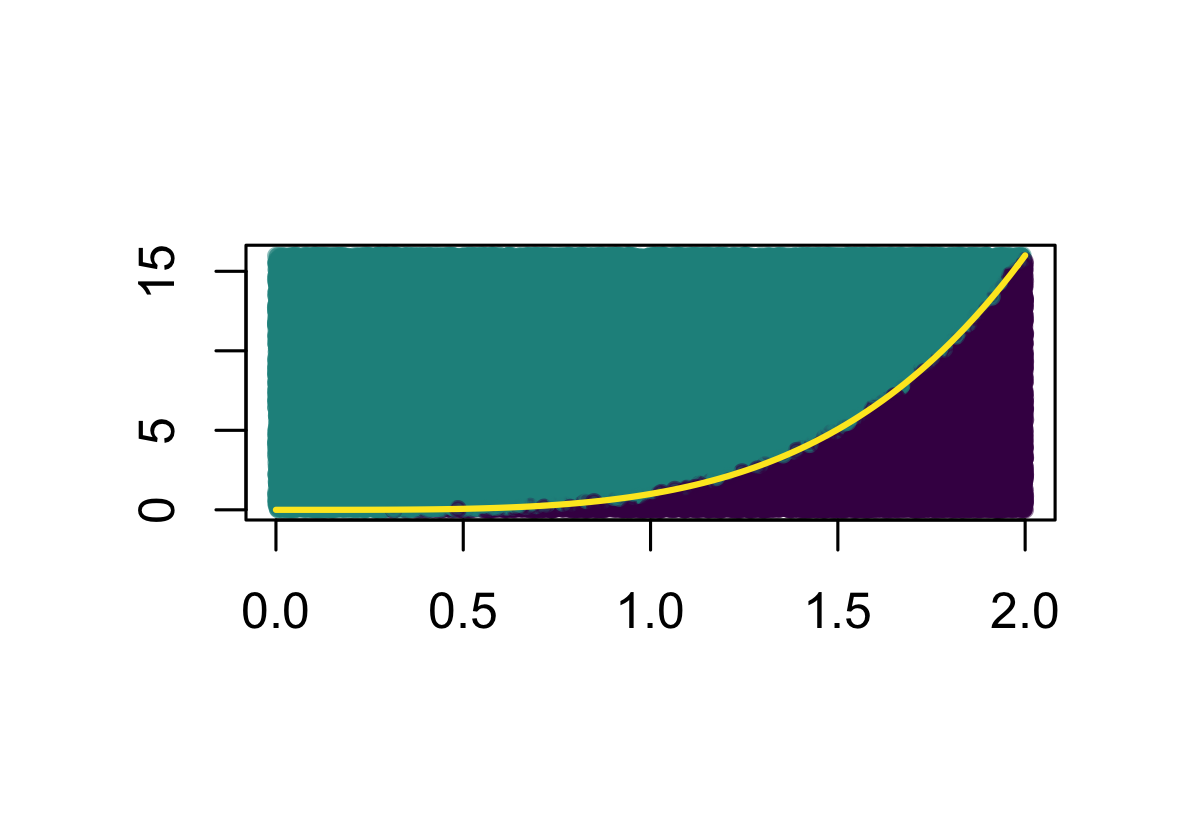
\includegraphics[width=10cm]{sim_hx.png}
\caption{Simulaciones de puntos en el rectángulo $\mathcal{R}$.}
\label{fig:sim_hx}
\end{figure}

La importancia de las técnicas de integración Monte Carlo en el contexto de inferencia estadística recae en que, si se tiene una distribución continua, muchas propiedades de esta distribución se pueden expresar como integrales. Esto es principalmente importante en inferencia bayesiana ya que muchas veces no interesa obtener la expresión explícita de las distribuciones posteriores, si no que únicamente se busca su valor esperado, varianza y otras cantidades de interés.

Si se tiene una distribución posterior para $\theta$ de la forma $\theta \sim F(\theta | \underline{x}_{(n)})$, donde $\underline{x}_{(n)}$ es una muestra observada de datos, entonces el valor esperado de $\theta| \underline{x}_{(n)}$ es
\begin{equation}
\label{eq:exp_theta}
E[\theta | \underline{x}_{(n)}] = \int_{\Theta} \theta \ dF(\theta | \underline{x}_{(n)}).
\end{equation}
Para calcular esta expresión de manera analítica se necesita la densidad posterior $$f(\theta | \underline{x}_{(n)}) = \frac{f(\underline{x}_{(n)} | \theta)\pi (\theta)}{\int_{\Theta} f(\underline{x}_{(n)} | \theta)\pi (\theta) \ d\theta}.$$ Si el espacio $\Theta$ es de dimensión uno, la integral en el denominador y la integral \eqref{eq:exp_theta} se pueden aproximar con métodos de cuadratura como la regla de Simpson o el método del trapecio (ver \citet{burden}). Sin embargo, a medida que crece la dimensión del espacio parametral, crece también la complejidad de la aproximación con los métodos de cuadratura hasta volverse prácticamente imposible. Es ahí cuando entran las técnicas de integración Monte Carlo. Se pueden obtener muestras de la distribución posterior de $\theta$ y aproximar el valor esperado con la media muestral.

Cuando la distribución posterior tiene una forma conocida que se puede simular con los métodos de las secciones \ref{sec:transformada} y \ref{aceptacion}, entonces la aproximación del valor esperado es directa. Sin embargo, en muchas ocasiones no es posible obtener simulaciones de la distribución posterior únicamente con los algoritmos mencionados anteriormente y es necesario recurrir a los métodos de Monte Carlo vía cadenas de Markov. La idea de los métodos de MCMC es simular cadenas de Markov cuya distribución estacionaria sea la distribución de interés y utilizar estas simulaciones para la aproximación de la esperanza. Primero se presenta algo de teoría sobre cadenas de Markov. En el capítulo \ref{elmodelo} se combinan los algoritmos presentados hasta ahora con métodos de MCMC para simular observaciones de una distribución posterior multivariada.

\newpage

\subsubsection*{Cadenas de Markov}
Esta sección contiene la teoría mínima indispensable de cadenas de Markov para entender los algoritmos de Monte Carlo vía cadenas de Markov. Por facilidad se introduce esta teoría para procesos estocásticos en tiempo discreto y con espacio de estados discreto. Para procesos en tiempo continuo y/o espacio de estados continuo, se recomienda consultar \citet{ross}.

\textbf{Definición.} Sea $\lbrace X_t, t \in \mathbb{N} \cup \lbrace 0 \rbrace \rbrace$ un proceso estocástico con espacio de estados discreto. Se dice que este proceso es una cadena de Markov si 
\begin{align*}
P\left( X_{t+1} = j | X_t = i, X_{t-1} = i_{t-1}, \dots, X_0 = i_0\right) &= P\left( X_{t+1} = j \ | \ X_t = i\right),
\end{align*}
esto es, \textit{si fijando el presente, el futuro no depende del pasado.}

Si $$P\left( X_{t+1} = j \ | \ X_t = i\right) = P_{ij},$$ independiente de $t$, se dice que la cadena de Markov tiene probabilidades de transición estacionarias. Una cadena de Markov con esta característica se dice que es homogénea. A partir de aquí, se hace referencia únicamente a cadenas homogéneas.

\textbf{Definición.} Se define la \textit{probabilidad de transición en n pasos}, denotada $P_{ij}^n$, como
\begin{align*}
P_{ij}^n &= P\left( X_{m+n} = j \ | \ X_{m} = i\right)\\
&= P\left( X_n = j \ | \ X_0 = i \right),
\end{align*}
donde la última igualdad se sigue de la homogeneidad de la cadena.

Se dice que el estado $j$ es accesible desde el estado $i$ si existe $n \in \mathbb{N}$ tal que $P_{ij}^n > 0$. Estos dos estados están \textbf{comunicados} si además existe $m \in \mathbb{N}$ tal que $P_{ji}^m > 0$. Que los estados $i$ y $j$ estén comunicados se denota
\begin{equation} \label{clase_eq}
i \leftrightarrow j.
\end{equation}

La comunicación de los estados define una relación de equivalencia (ver \citet{ross}) y de esta forma dos estados comunicados pertenecen a una misma clase de equivalencia. Por las propiedades de estas relaciones, las clases definidas solamente pueden ser iguales o disjuntas. Se dice que una cadena de Markov es \textbf{irreducible} si su espacio de estados cuenta con una única clase de equivalencia.

\textbf{Definición.} Se define el \textit{tiempo de primer regreso al estado i} como $$T_i = \min_{t>0} \lbrace X_0 = i, X_t = i \rbrace.$$

Si $P\left( T_i < \infty \right) = 1 $ entonces se dice que el estado $i$ es \textbf{recurrente}. En otro caso, se dice que el estado $i$ es transitorio. Además, si $i$ es un estado recurrente, se dice que éste es \textbf{recurrente positivo} si $E\left[T_i\right] < \infty$. En otro caso, se dice que $i$ es recurrente nulo.

\textbf{Definición.} Se define el periodo del estado $i$, denotado $d(i)$, como el máximo común divisor de $\lbrace n\in \mathbb{N}: P_{ii}^n > 0\rbrace.$ Si $d(i)=1$, se dice que el estado $i$ es \textbf{aperiódico}.

El siguiente resultado muestra que para una cadena de Markov irreducible, si el estado $i$ es recurrente positivo y aperiódico, entonces todos los demás estados también lo son. La demostración se puede consultar en \citet{ross}.

\begin{proposition}
Las propiedades de recurrencia, recurrencia positiva, recurrencia nula y aperiodicidad son comunes a una clase de equivalencia definida por \eqref{clase_eq}.
\end{proposition}

\textbf{Definición.} Se dice que una cadena de Markov es ergódica si es irreducible y todos sus estados son recurrentes positivos y aperiódicos.

El teorema \ref{teo:ergodic} es un resultado importante en la teoría de cadenas de Markov. En él se establecen las condiciones bajo las cuales una cadena cuenta con una \textit{distribución límite}.

\begin{theorem}
\label{teo:ergodic}
Sea $P=[P_{ij}]$ la matriz de transición de una cadena de Markov ergódica. Entonces existe un único vector $\pi = (\pi_1, \pi_2, \dots)^\prime$ tal que
\begin{equation} \label{dist_limite}
\lim_{n \to \infty}P^n = [\pi \ \pi \dots \pi \dots ]^\prime.
\end{equation}
A $\pi$ se le conoce como la \textbf{distribución estacionaria} de la cadena ergódica.
\end{theorem}

Si se quieren obtener muestras de una densidad $f$, difíciles o imposibles de obtener con el método de la transformada inversa o con métodos de aceptación y rechazo, la idea de los algoritmos de MCMC es crear una cadena de Markov ergódica cuya distribución estacionaria sea $f$ y simular observaciones de esta cadena. En el límite, estas observaciones siguen una distribución dada por $f$.

En esta sección se presentaron las ideas únicamente con cadenas de Markov con espacio de estados discreto. Sin embargo algunas propiedades como la irreducibilidad, aperiodicidad, la recurrencia y la existencia de una distribución estacionaria se pueden trasladar a cadenas con espacio de estados continuo, que son las que se utilizan más adelante. En el caso continuo, en vez de contar con una matriz de transición, se tiene un \textit{kernel} de transición. El kernel de transición, denotado $P(x, \mathcal{A})$, es una función de distribución condicional que representa la probabilidad de moverse de $x$ a un punto en el conjunto $\mathcal{A}$ \citep{chib_mh}.

\subsubsection*{Muestreador de Gibbs}
En los siguientes dos apartados se introducen dos de los algoritmos más importantes de Monte Carlo vía cadenas de Markov, el muestreador de Gibbs y el algoritmo de Metropolis-Hastings. Aunque el muestreador de Gibbs es un caso especial del algoritmo de Metropolis-Hastings, se habla antes del primero porque el algoritmo de Metropolis-Hastings no había sido popular en la comunidad estadística hasta la aparición del muestreador de Gibbs. Se introduce primero un poco de contexto histórico. Para un relato más detallado de este contexto se recomienda leer \citet{bertsch}.

Para 1980, las bases teóricas de la inferencia bayesiana estaban bien establecidas y desarrolladas por estadísticos como Leonard Jimmie Savage, Bruno de Finetti y Dennis Lindley. Sin embargo, el uso de estas técnicas estaba limitado por la dificultad de realizar todos los cálculos a mano. Las primeras computadoras hacían que la información fuera más accesible, pero esto a su vez hizo que creciera la dimensión de los espacios parametrales de interés, por lo que resultaba prácticamente imposible estudiar distribuciones a priori, verosimilitudes y distribuciones posteriores en estos espacios.

El muestreador de Gibbs \textit{(Gibbs sampler)} fue introducido por los hermanos Stuart y Donald Geman como una herramienta para el reconocimiento de imágenes en 1984. A pesar de esto, tampoco fue muy utilizado en la práctica ya que el gran número de pixeles en una imagen era inmanejable para las computadoras de la época. Algún tiempo después se supo que el matemático ruso Valentin Fedorovich Turchin había descubierto el muestreador de Gibbs en 1971 pero su artículo solamente apareció en publicaciones rusas y no tuvo gran difusión.

El muestreador de Gibbs como un método de simulación se introdujo en \citet{gelfand_smith}, donde se utiliza el algoritmo de los hermanos Geman para obtener muestras de distribuciones marginales a partir de distribuciones condicionales. Alan Gelfand explicó que el muestreador de Gibbs toma el problema de simular observaciones de una distribución de gran dimensión y lo divide en pequeños pedazos que son fáciles de resolver. Estos pedazos son obtener muestras de distribuciones condicionales. A continuación se explica cómo hacer esta división.

Se toma primero un caso con dos variables aleatorias, $X$ y $Y$. La idea del muestreador de Gibbs es simular observaciones de la distribución conjunta $f_{X, Y}$ utilizando simulaciones de las distribuciones condicionales $f_{X|Y}$ y $f_{Y|X}$, suponiendo que estas condicionales son conocidas y fáciles de simular. El algoritmo en el caso bivariado es como sigue. Primero se fijan valores iniciales $x^{(0)}, y^{(0)}$. Luego, en la iteración $t$ el algoritmo es:
\begin{enumerate}
\item Simular $Y^{(t)} \sim Y|X = x^{(t-1)}$.
\item Simular $X^{(t)} \sim X|Y = y^{(t)}$.
\end{enumerate}

Como se menciona en \citet{casella_gs}, bajo ciertas condiciones generales la distribución de la sucesión $\lbrace X_t, Y_t \rbrace$ converge a la distribución conjunta $f_{X, Y}$ y por lo tanto se cumple que marginalmente $\lbrace X_t \rbrace$ converge a $f_X$ y $\lbrace Y_t \rbrace$ converge a $f_Y$.

Para ilustrar el algoritmo se presenta un ejemplo de \citet{casella}. Se tiene que el vector $(X, Y)$ sigue una distribución normal bivariada con vector de medias $\mu = [0, 0]^\prime$, varianzas $\sigma^2_X = \sigma^2_Y = 1$ y covarianza $\sigma_{XY} = 0.8$. Así, marginalmente se cumple que $X \sim \mathcal{N}(0, 1)$ y $Y \sim \mathcal{N}(0, 1)$. El objetivo es simular de estas distribuciones utilizando el muestreador de Gibbs. Para esto, se necesitan las distribuciones condicionales, las cuales están dadas por $$Y|X = x \sim \mathcal{N}(0.8 x, 0.36)$$ y $$X|Y = y \sim \mathcal{N}(0.8 y, 0.36).$$

Se establecen los valores iniciales $x^{(0)}, y^{(0)}$ y se corre el algoritmo por 10 mil iteraciones. En la figura \ref{fig:gs_norm} se grafican las distribuciones marginales, comparándolas contra la densidad normal estándar verdadera y se visualiza la correlación con un diagrama de dispersión. El código para generar las simulaciones se muestra en el cuadro \ref{cod:gs}.

\begin{table}[htb]
\begin{lstlisting}
nsim <- 1e4

x <- vector(mode = "double", length = nsim)
y <- vector(mode = "double", length = nsim)

set.seed(42)

x[1] <- rnorm(1)
y[1] <- rnorm(1)

rho <- 0.8

for (i in 1:(nsim - 1)) {
  y[i + 1] <- rnorm(1, mean = rho * x[i], sd = sqrt((1 - rho^2)))
  x[i + 1] <- rnorm(1, mean = rho * y[i + 1], sd = sqrt((1 - rho^2)))
}
\end{lstlisting}
\caption{Código para simular observaciones de $(X, Y)$ utilizando el muestreador de Gibbs en R. }
\label{cod:gs}
\end{table}

\begin{figure}[!p]
    \centering
    \begin{subfigure}[t]{0.45\textwidth}
        \centering
        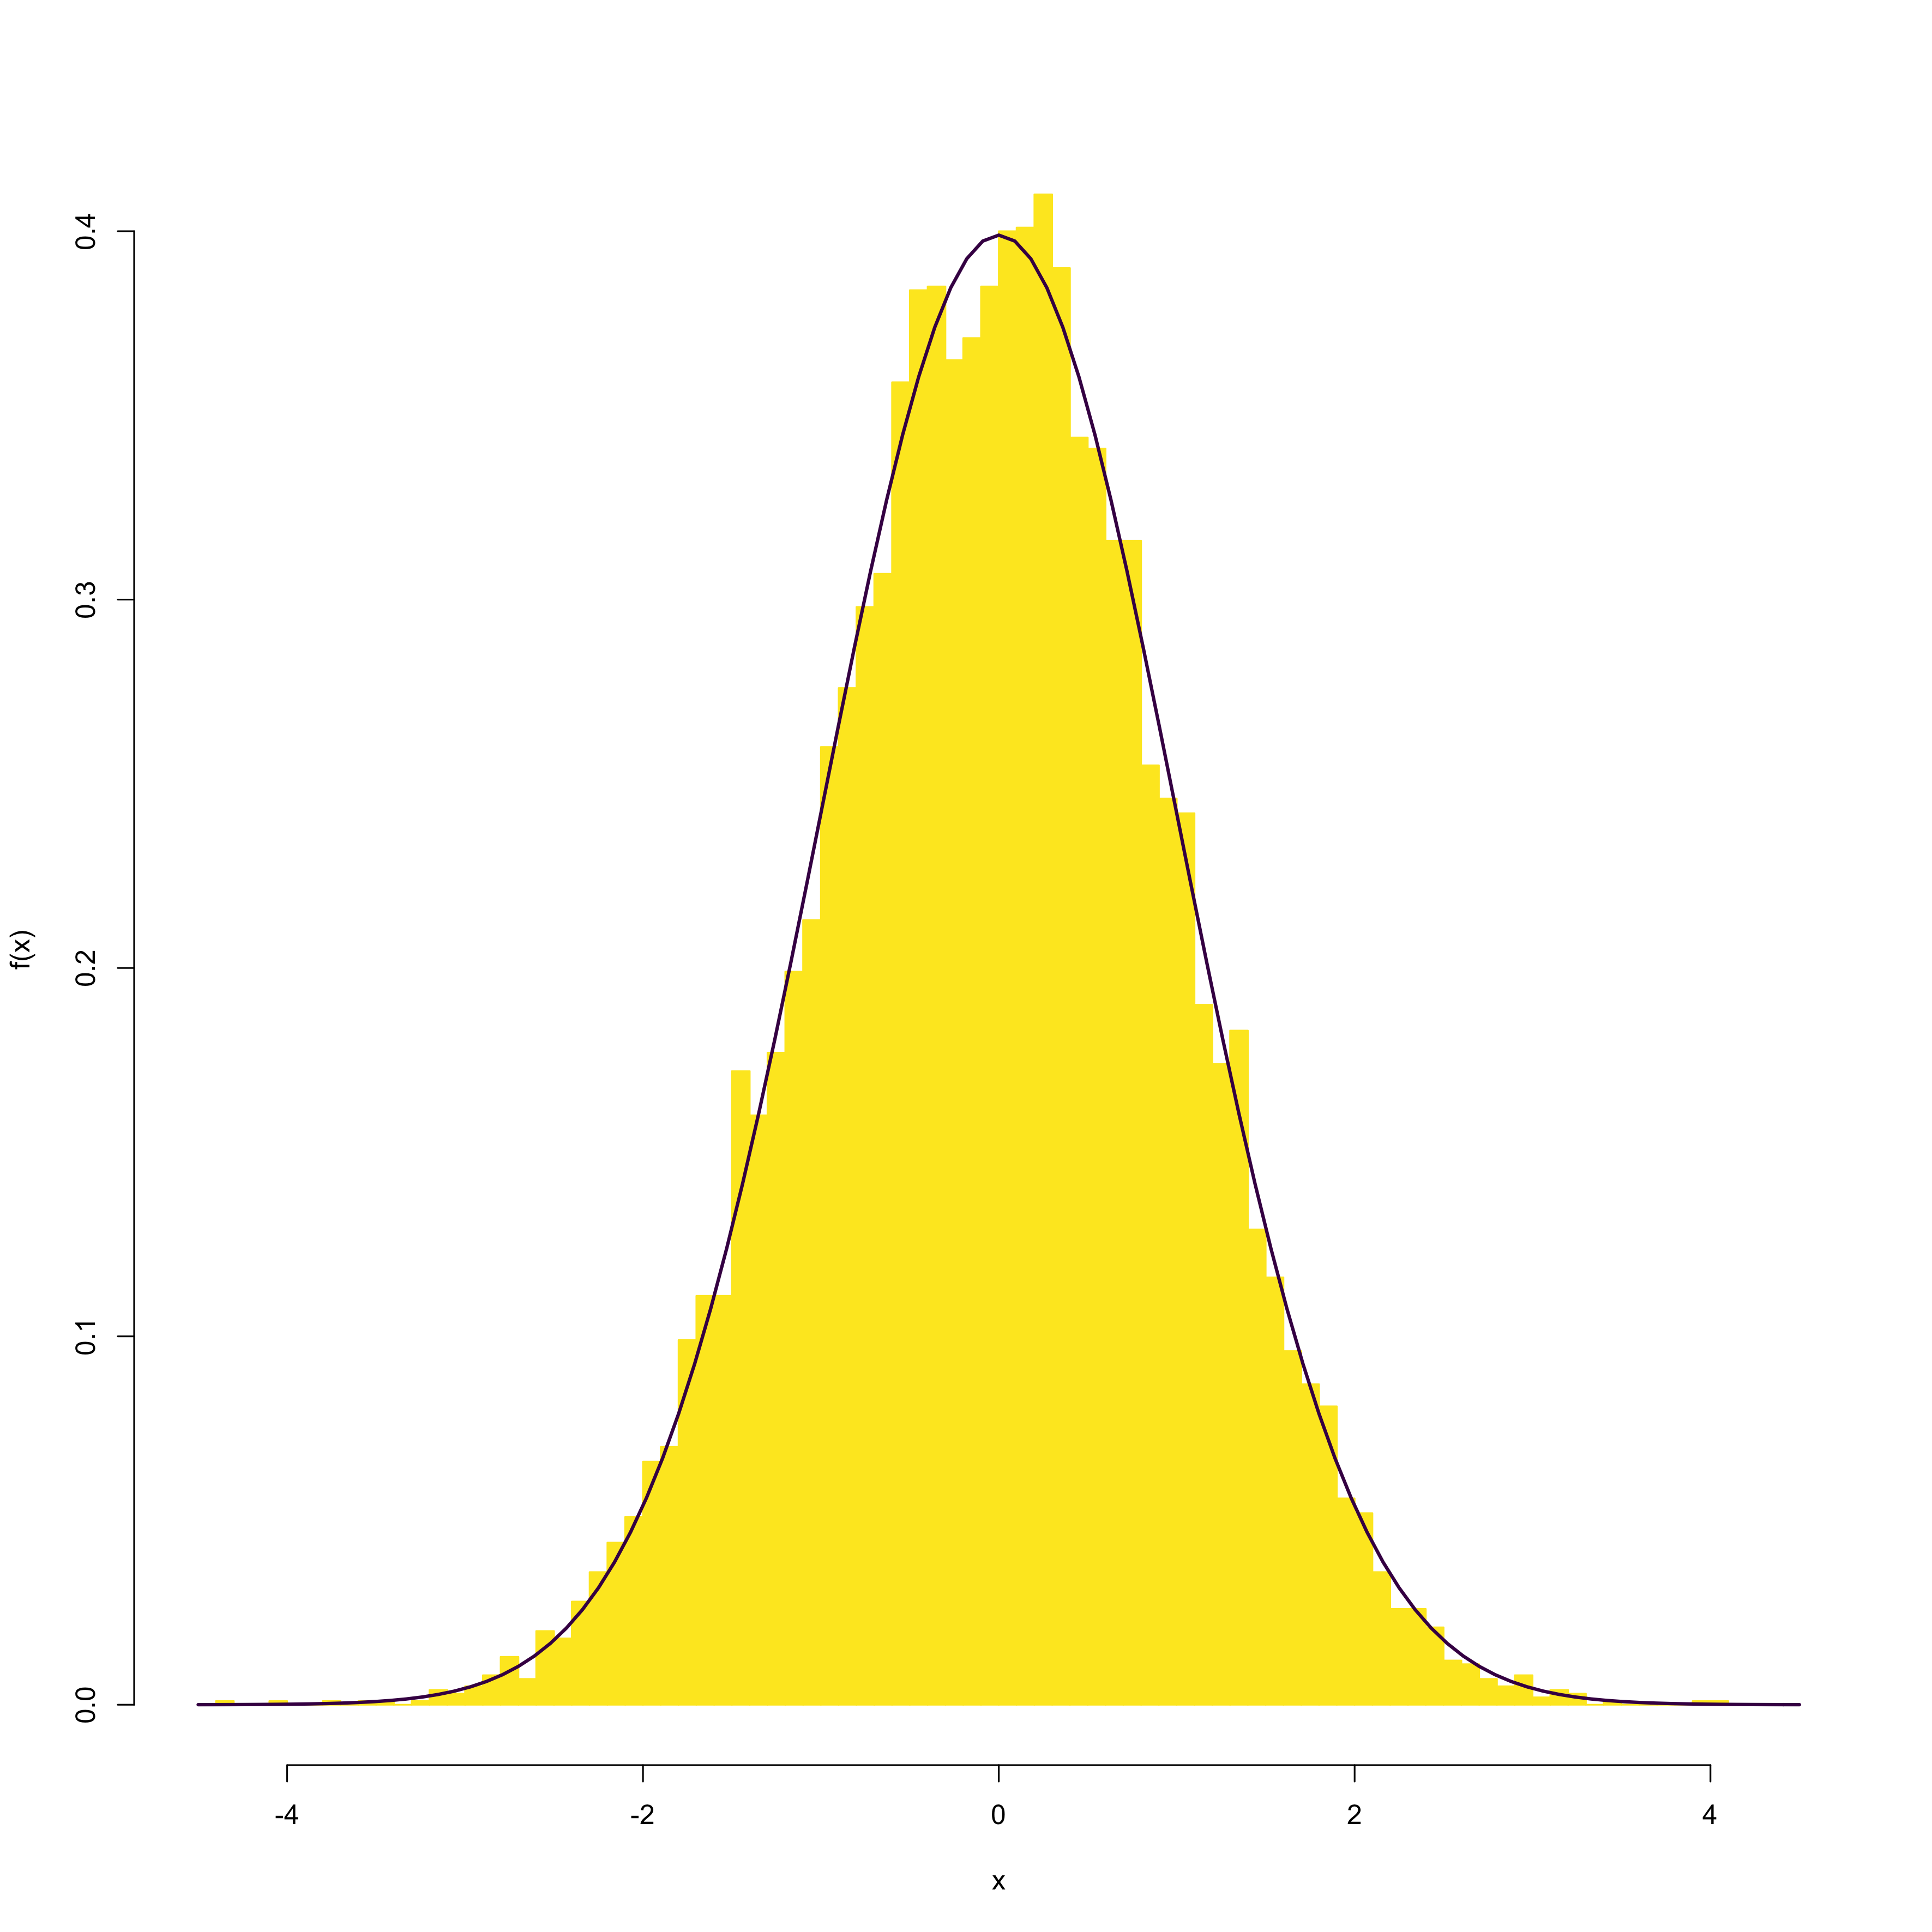
\includegraphics[width=\linewidth]{x_norm.png} 
        \caption{Distribución marginal $f_X$.} \label{fig:xnorm}
    \end{subfigure}
    \hfill
    \begin{subfigure}[t]{0.45\textwidth}
        \centering
        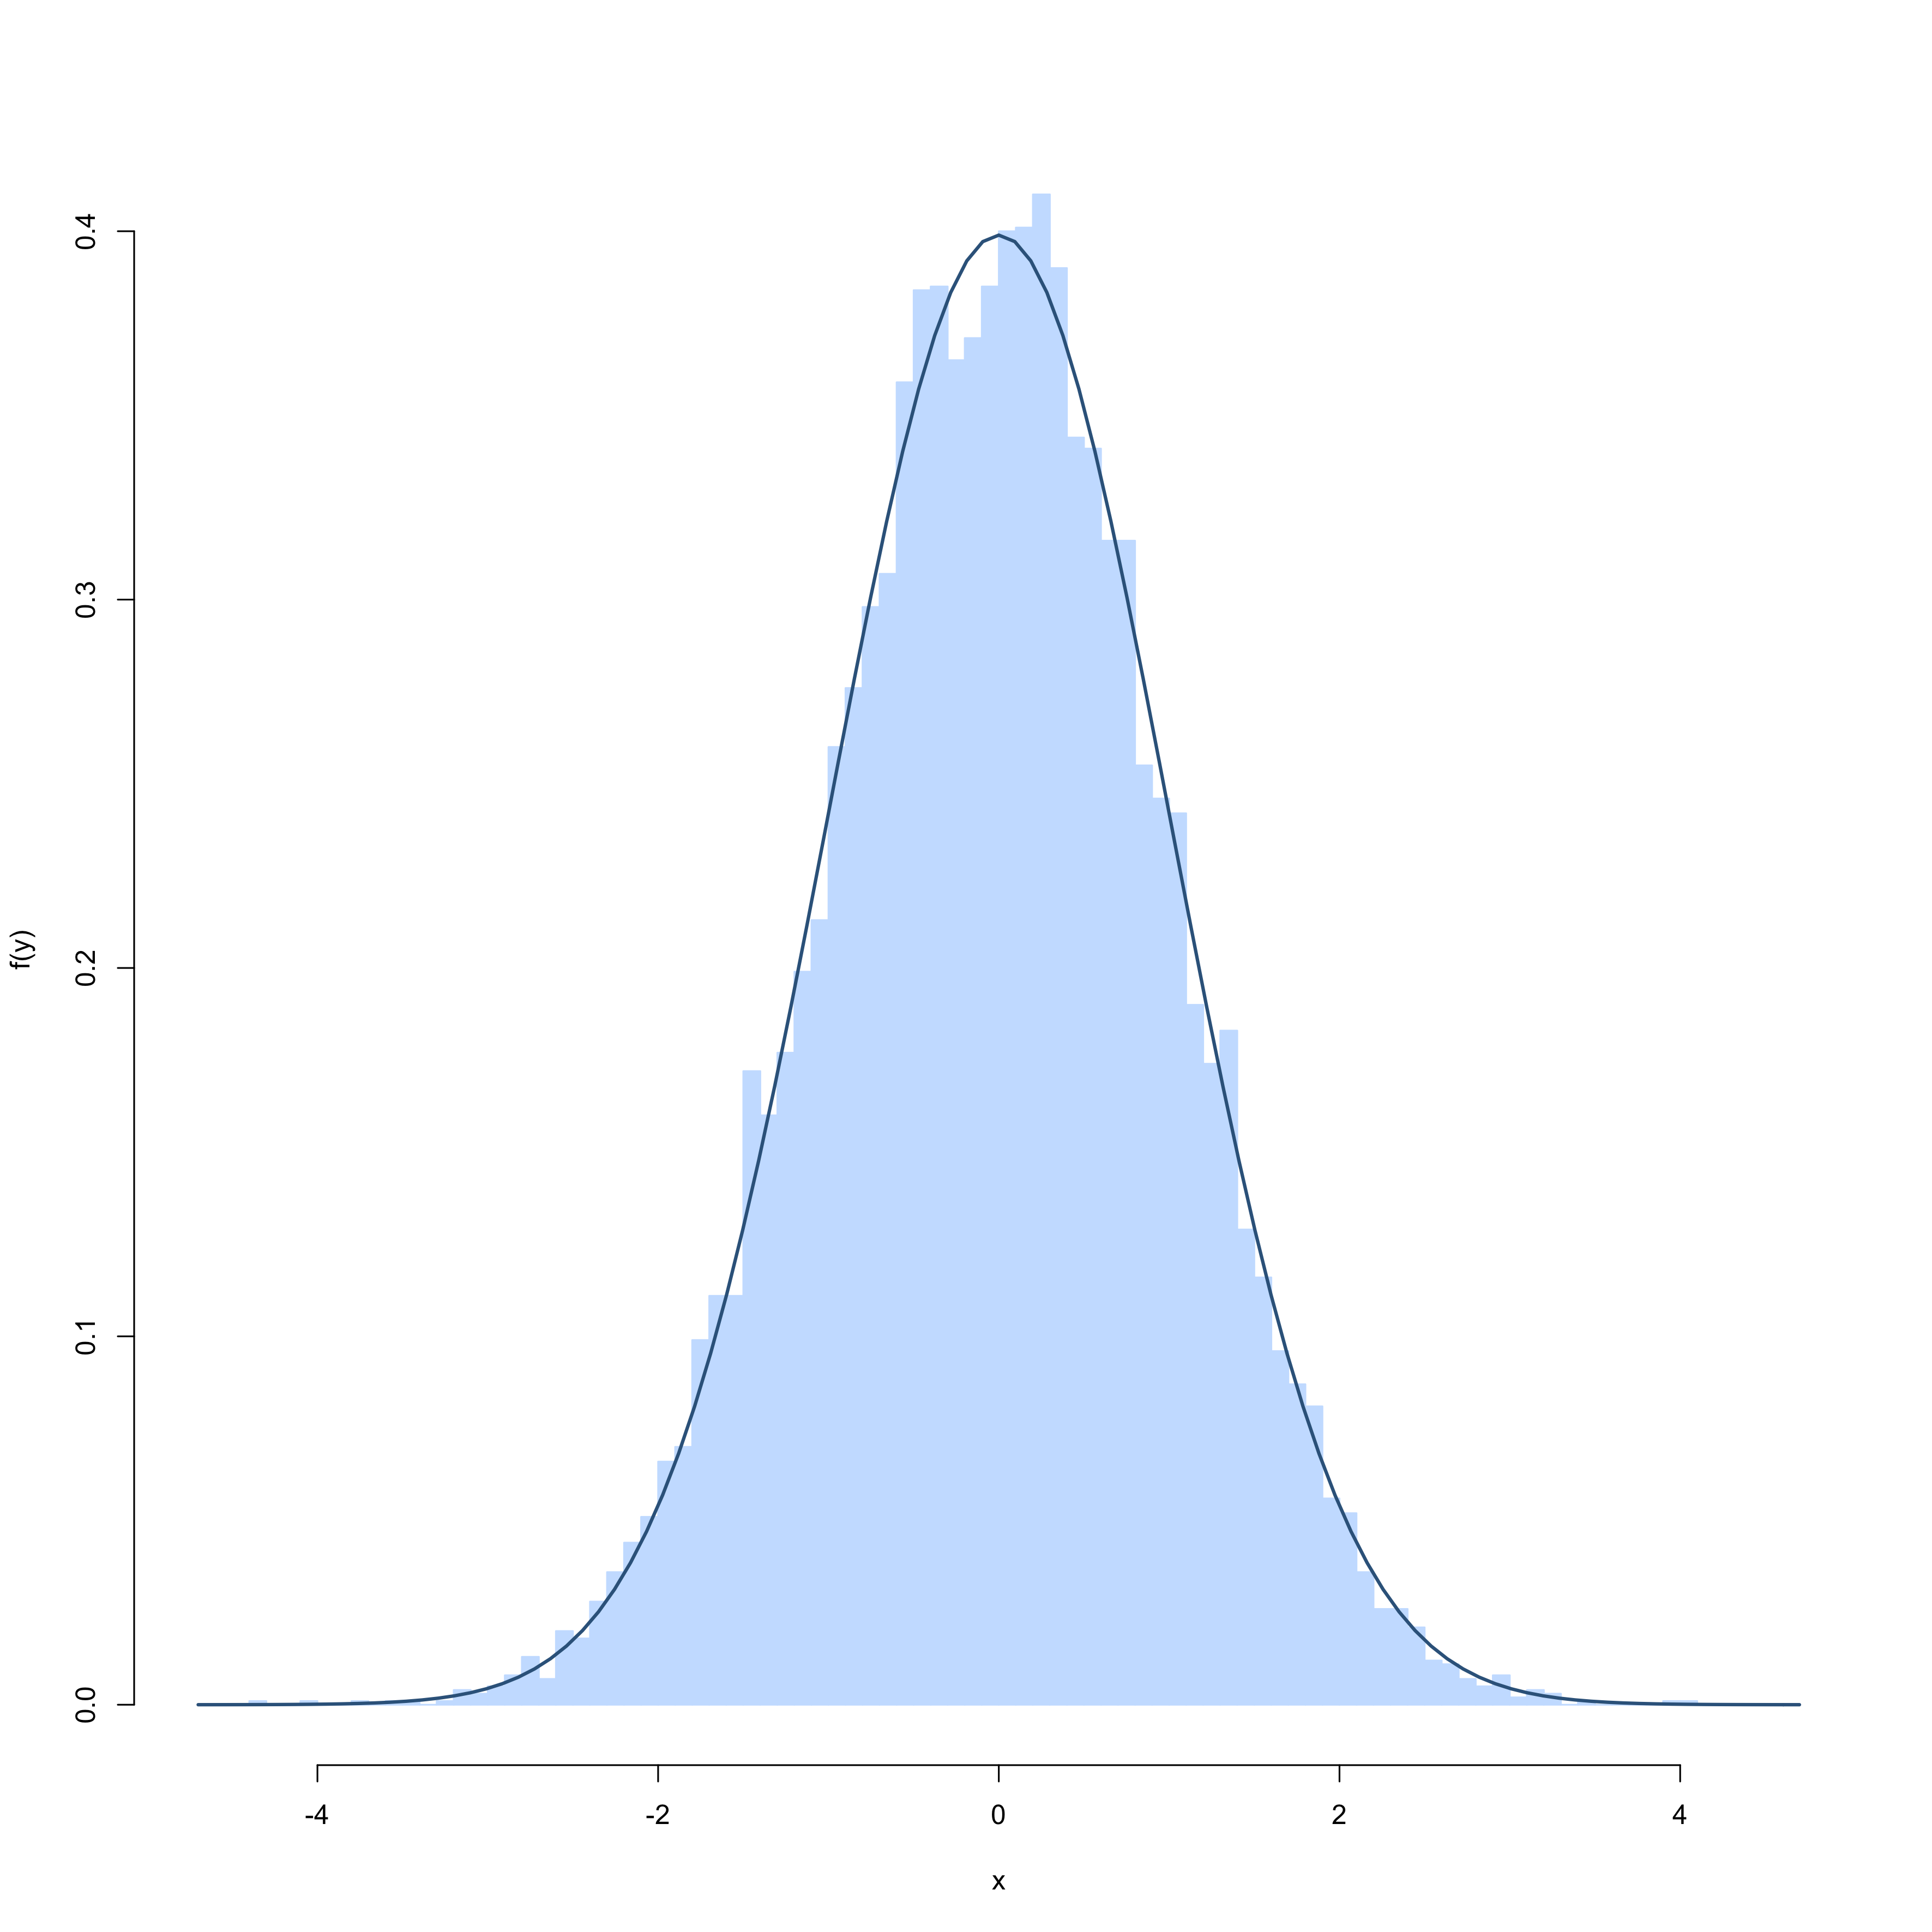
\includegraphics[width=\linewidth]{y_norm.png} 
        \caption{Distribución marginal $f_Y$.} \label{fig:ynorm}
    \end{subfigure}

    \vspace{0.2cm}
    \begin{subfigure}[t]{\textwidth}
    \centering
        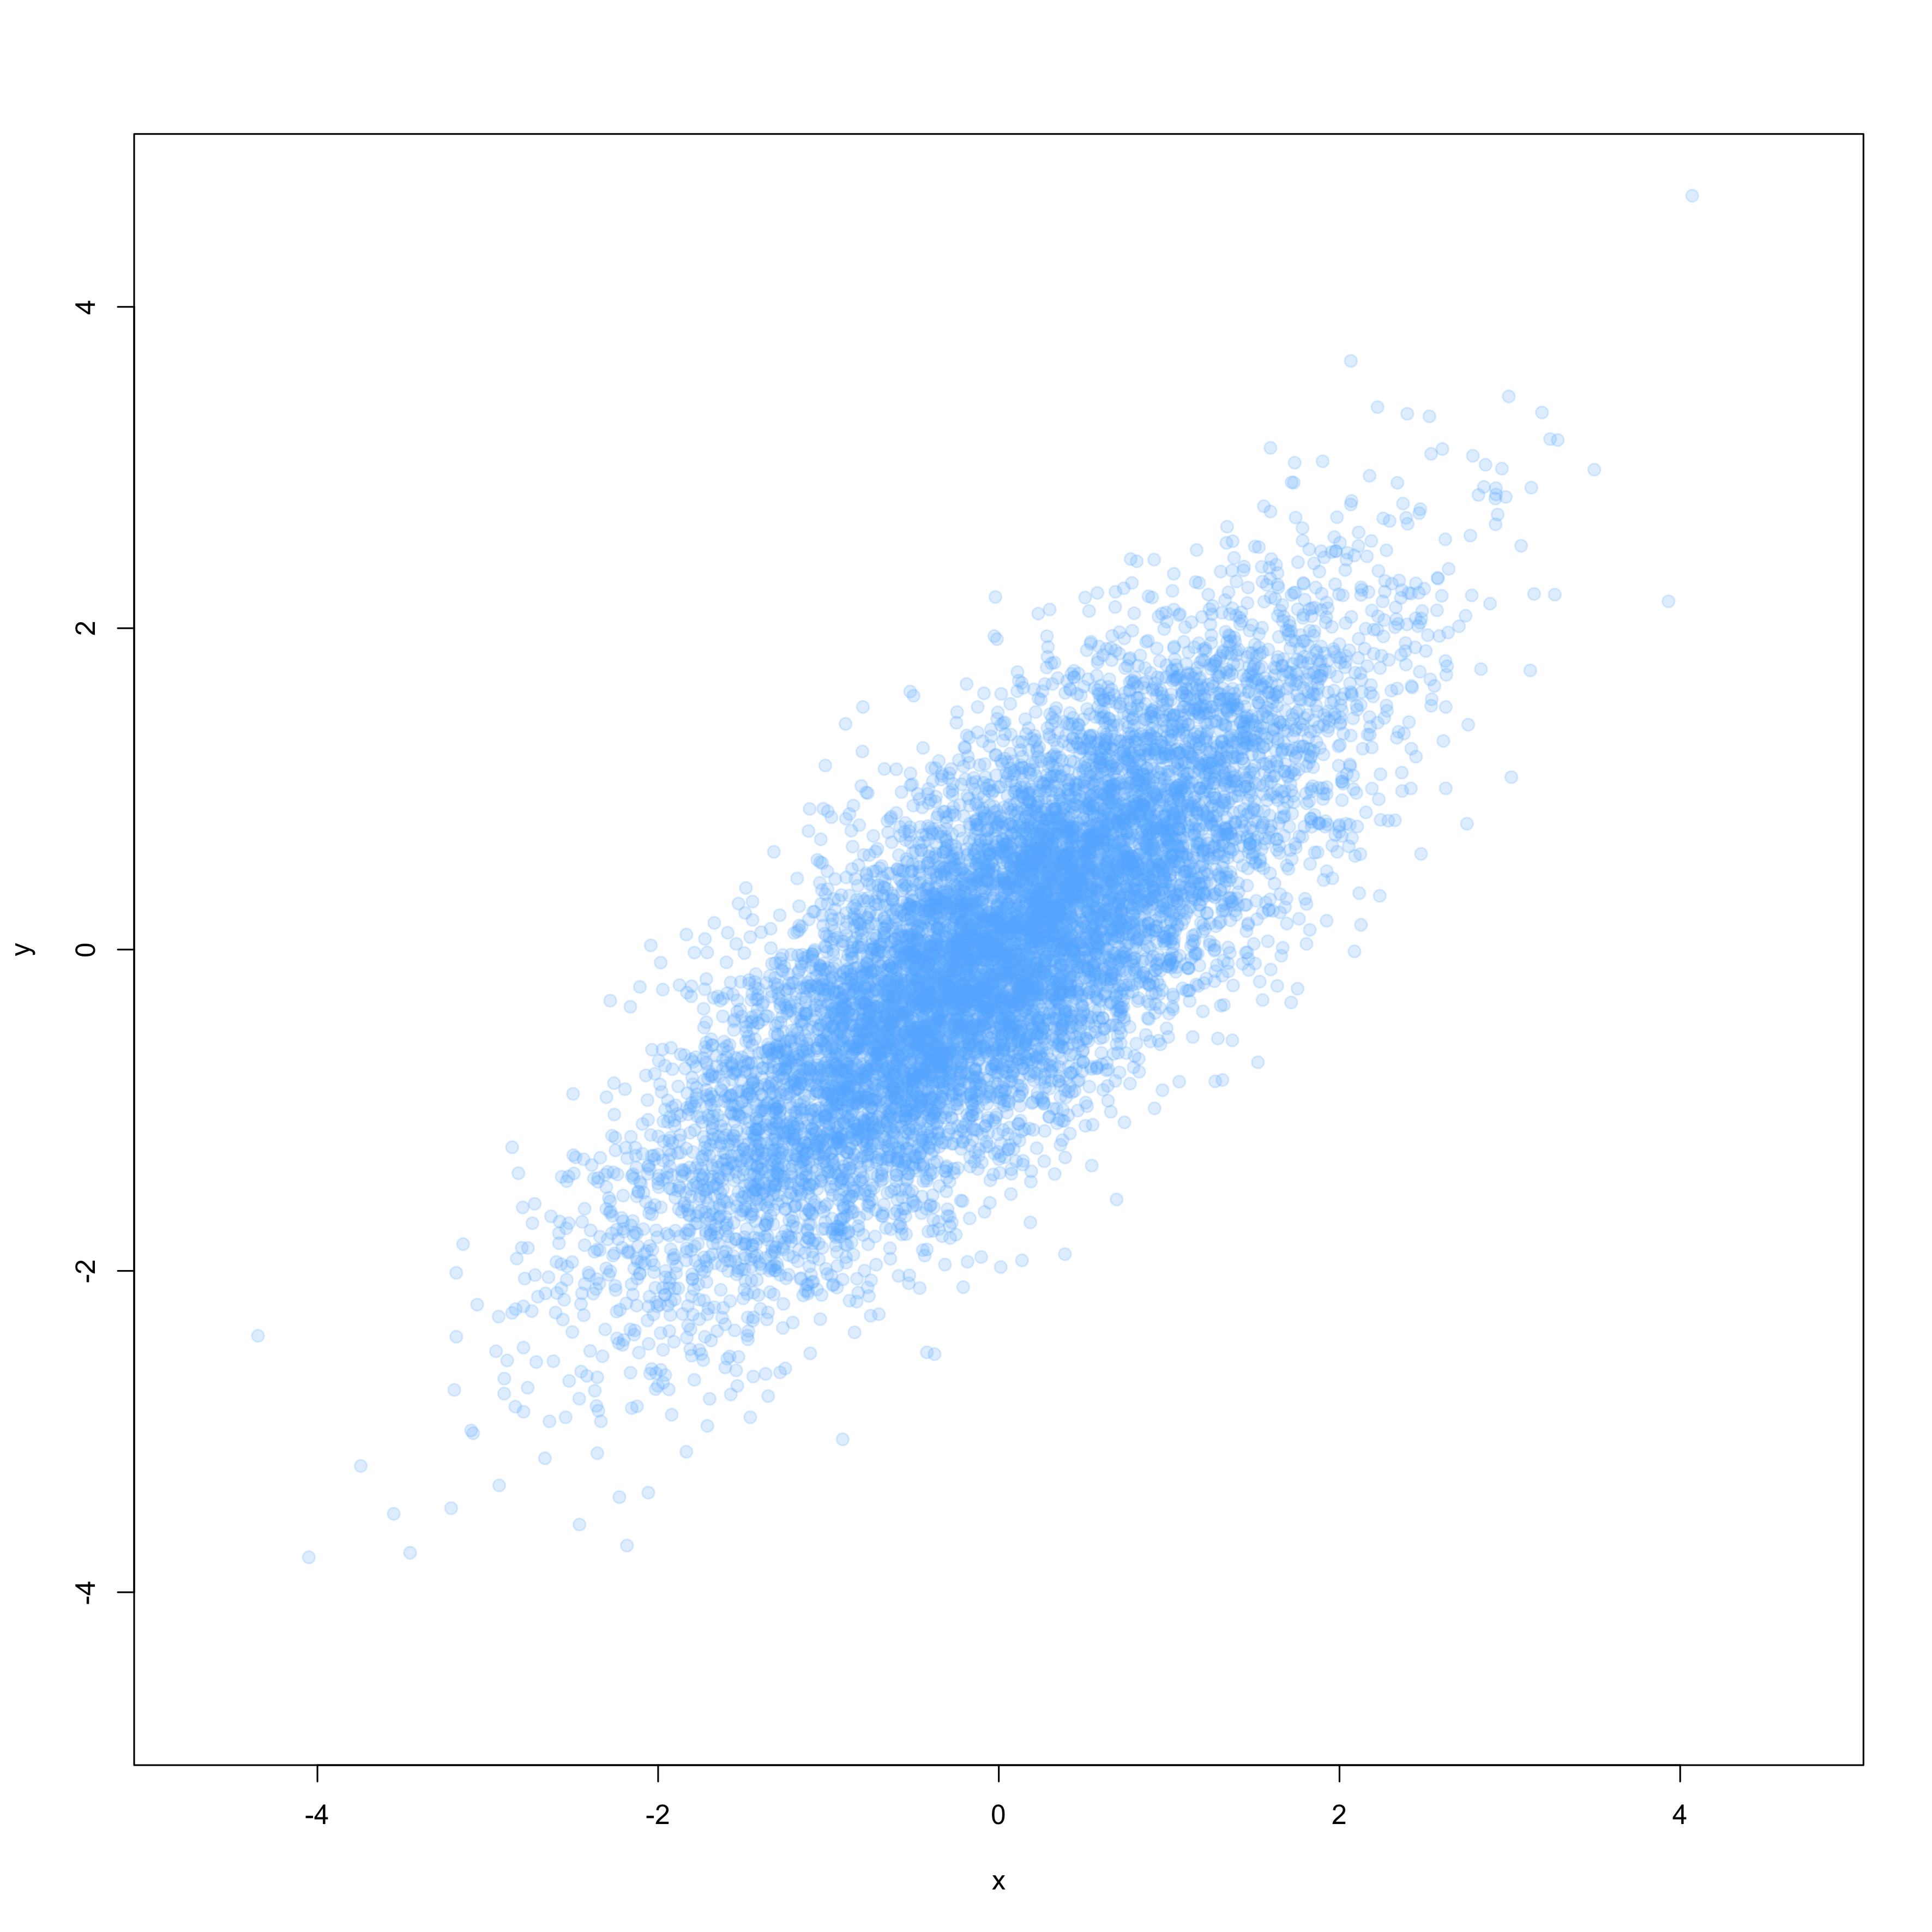
\includegraphics[width=9cm]{bivnorm.png} 
        \caption{Diagrama de dispersión de $(X, Y)$.} \label{fig:bivnorm}
    \end{subfigure}
    \caption{Simulación de un vector normal utilizando el muestreador de Gibbs.}
    \label{fig:gs_norm}
\end{figure}

Como se puede ver en los páneles \ref{fig:xnorm} y \ref{fig:ynorm} de la figura \ref{fig:gs_norm}, las distribuciones marginales empíricas de los procesos $\lbrace X_t \rbrace$ y $\lbrace Y_t \rbrace$ son muy similares a las de una normal estándar, mientras que el diagrama de dispersión \ref{fig:bivnorm} muestra la forma elíptica característica de una distribución normal bivariada con componentes correlacionadas.

\newpage

La extensión del muestreador de Gibbs a mayores dimensiones se hace de la misma manera. Supóngase que se tiene un vector aleatorio $\theta$, dividido en $p$ subvectores $\theta = (\theta_1, \theta_2, \dots, \theta_p)$. Si se conocen todas las distribuciones condicionales de la forma $f_{\theta_i | \theta_{-i}},$ $i \in \lbrace 1, 2, \dots, p\rbrace$ entonces se pueden simular observaciones de las densidades marginales con el siguiente algoritmo. Primero, se establecen valores iniciales $\theta^{(0)} = (\theta_1^{(0)}, \theta_2^{(0)}, \dots, \theta_p^{(0)})$. Luego, la iteración $t$ del algoritmo es:
\begin{itemize}
\item[] 1. Simular $\theta_1^{(t)} | \theta_2^{(t-1)}, \dots, \theta_p^{(t-1)}$
\item[] 2. Simular $\theta_2^{(t)} | \theta_1^{(t)}, \theta_3^{(t-1)}, \dots, \theta_p^{(t-1)}$
\item[] $\dots$
\item[] p. Simular $\theta_p^{(t)} | \theta_1^{(t)}, \theta_2^{(t)}, \dots, \theta_{p-1}^{(t)}$
\end{itemize}

En \citet{geman} se muestran las condiciones bajo las cuales la distribución del proceso $\lbrace (\theta_1, \theta_2, \dots, \theta_p)_t\rbrace$ converge a la distribución conjunta $f_{\theta}$ \textbf{sin importar los valores iniciales} y por lo tanto, la distribución del proceso $\lbrace \theta_i^t \rbrace$ converge a la distribución marginal $f_{\theta_i}$ \citep{gelfand_smith}. Para estudiar las propiedades matemáticas de esta convergencia resulta más sencillo estudiar las propiedades del algoritmo de Metropolis-Hastings y entender el muestreador de Gibbs como un caso particular de éste. Es importante notar que si los subvectores en que se divide el vector $\theta$ son en realidad cada uno de sus elementos, entonces todas las simulaciones que se deben realizar en el algoritmo son de distribuciones univariadas, lo cual suele simplificar la programación.

Una de las mayores facilidades del muestreador de Gibbs es que es común encontrar la especificación de distribuciones conjuntas a través de las condicionales cuando se trabaja con modelos jerárquicos. Esto es ejemplificado por diversos autores como \citet{casella}, \citet{gelman} y \citet{gelfand_smith}. Otra ventaja es que el muestreador de Gibbs se puede utilizar para trabajar con modelos de variables latentes. Estos son modelos expresados de la forma $$f(x| \theta) = \int_\Xi f(x, \xi | \theta) \ d\xi,$$ donde $\xi$ es la variable latente (no observable) y $\Xi$ su soporte. En la sección \ref{elmodelo} se utilizan estos modelos para describir la correlación entre tiempos de fallo y para trabajar con observaciones no exactas.

Se presenta un ejemplo de un modelo jerárquico para ilustrar el muestreador de Gibbs con más de dos variables \citep{casella_gs}. La especificación del modelo es como sigue:
\begin{itemize}
\item $\omega|\theta, \gamma \sim Binomial(\gamma, \theta)$,
\item $\theta | \omega, \gamma \sim Be(\omega + \alpha, \gamma - \omega + \beta)$,
\item $\gamma | \omega, \theta \propto e^{-\lambda(1-\theta)}\frac{[(1-\theta)\lambda]}{(\gamma - \omega)!}^{\gamma - \omega} \mathbb{I}_{\lbrace \omega, \omega + 1, \dots \rbrace}(\gamma),$
\end{itemize}
donde $\alpha$, $\beta$ y $\lambda$ son hiperparámetros constantes. La distribución condicional $\gamma | \omega, \theta$ es una Poisson con parámetro $\lambda(1-\theta)$ y el soporte desplazado a $\lbrace \omega, \omega + 1, \dots \rbrace$. Para obtener muestras de esta distribución se puede simular $\delta \sim Po(\lambda(1-\theta))$ y hacer $\gamma = \delta + \omega$. Primero, se establecen los valores iniciales $\omega^{(0)}$, $\theta^{(0)}$ y $\gamma^{(0)}$. En el cuadro \ref{cod:gs_hier} se incluye el código para realizar las simulaciones. Se utilizan los valores de los hiperparámetros $\alpha = 2$, $\beta = 4$ y $\lambda = 16$ y se realizan 10 mil iteraciones.

\begin{table}[!htb]
\begin{lstlisting}
set.seed(42)
nsim <- 1e4

alpha <- 2
beta <- 4
lambda <- 16

omega <- vector(mode = "double", length = nsim)
gamma <- vector(mode = "double", length = nsim)
theta <- vector(mode = "double", length = nsim)

omega[1] <- rbinom(n = 1, size = 5, prob = 0.5)
theta[1] <- rbeta(n = 1, shape1 = alpha, shape2 = beta)
gamma[1] <- rpois(n = 1, lambda = 4) + omega[1]

for (i in 2:nsim) {
  omega[i] <- rbinom(n = 1, size = gamma[i - 1], prob = theta[i - 1])
  theta[i] <- rbeta(
    n = 1,
    shape1 = omega[i] + alpha,
    shape2 = gamma[i - 1] - omega[i] + beta
    )
  gamma[i] <- omega[i] + rpois(n = 1, lambda = lambda * (1 - theta[i]))
}
\end{lstlisting}
\caption{Código para simular observaciones de $(\omega, \theta, \gamma)$ en R.}
\label{cod:gs_hier}
\end{table}

\begin{figure}[!p]
    \centering
    \begin{subfigure}[t]{0.45\textwidth}
        \centering
        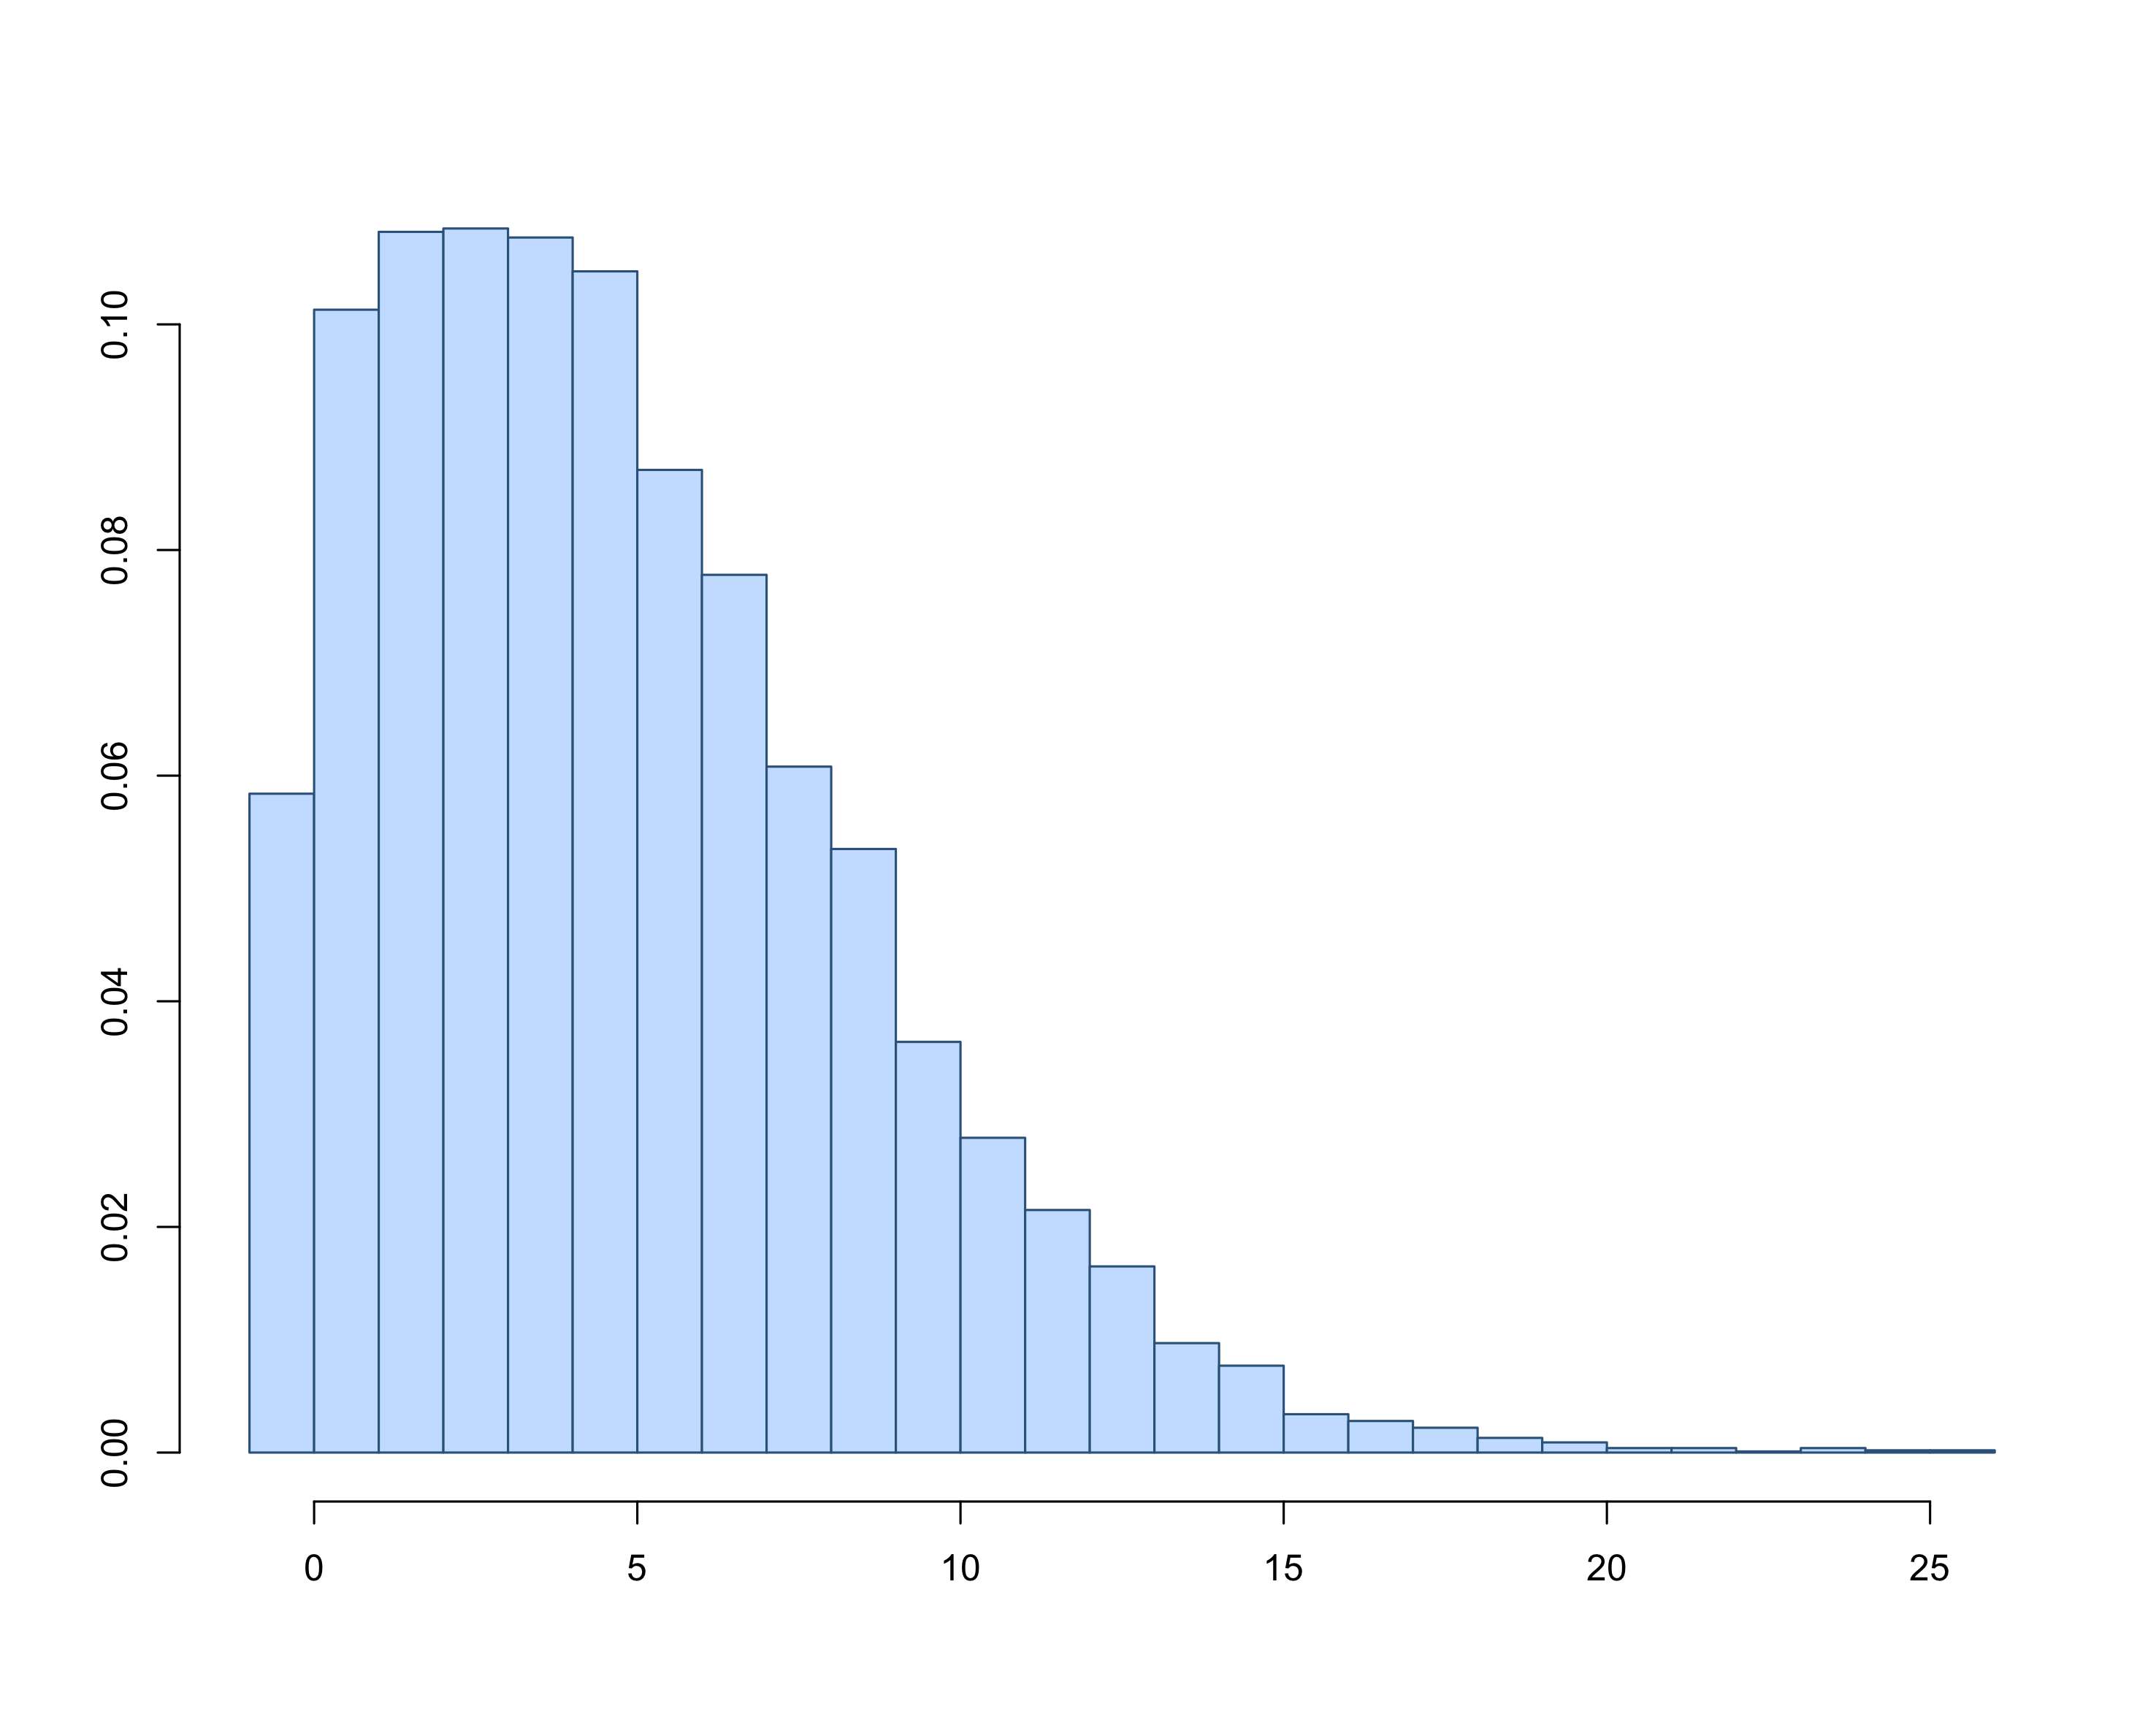
\includegraphics[width=\linewidth]{hier_hist_omega.png} 
        \caption{Distribución marginal $f_\omega$.} \label{fig:hier_hist_omega}
    \end{subfigure}
    \hfill
    \begin{subfigure}[t]{0.45\textwidth}
        \centering
        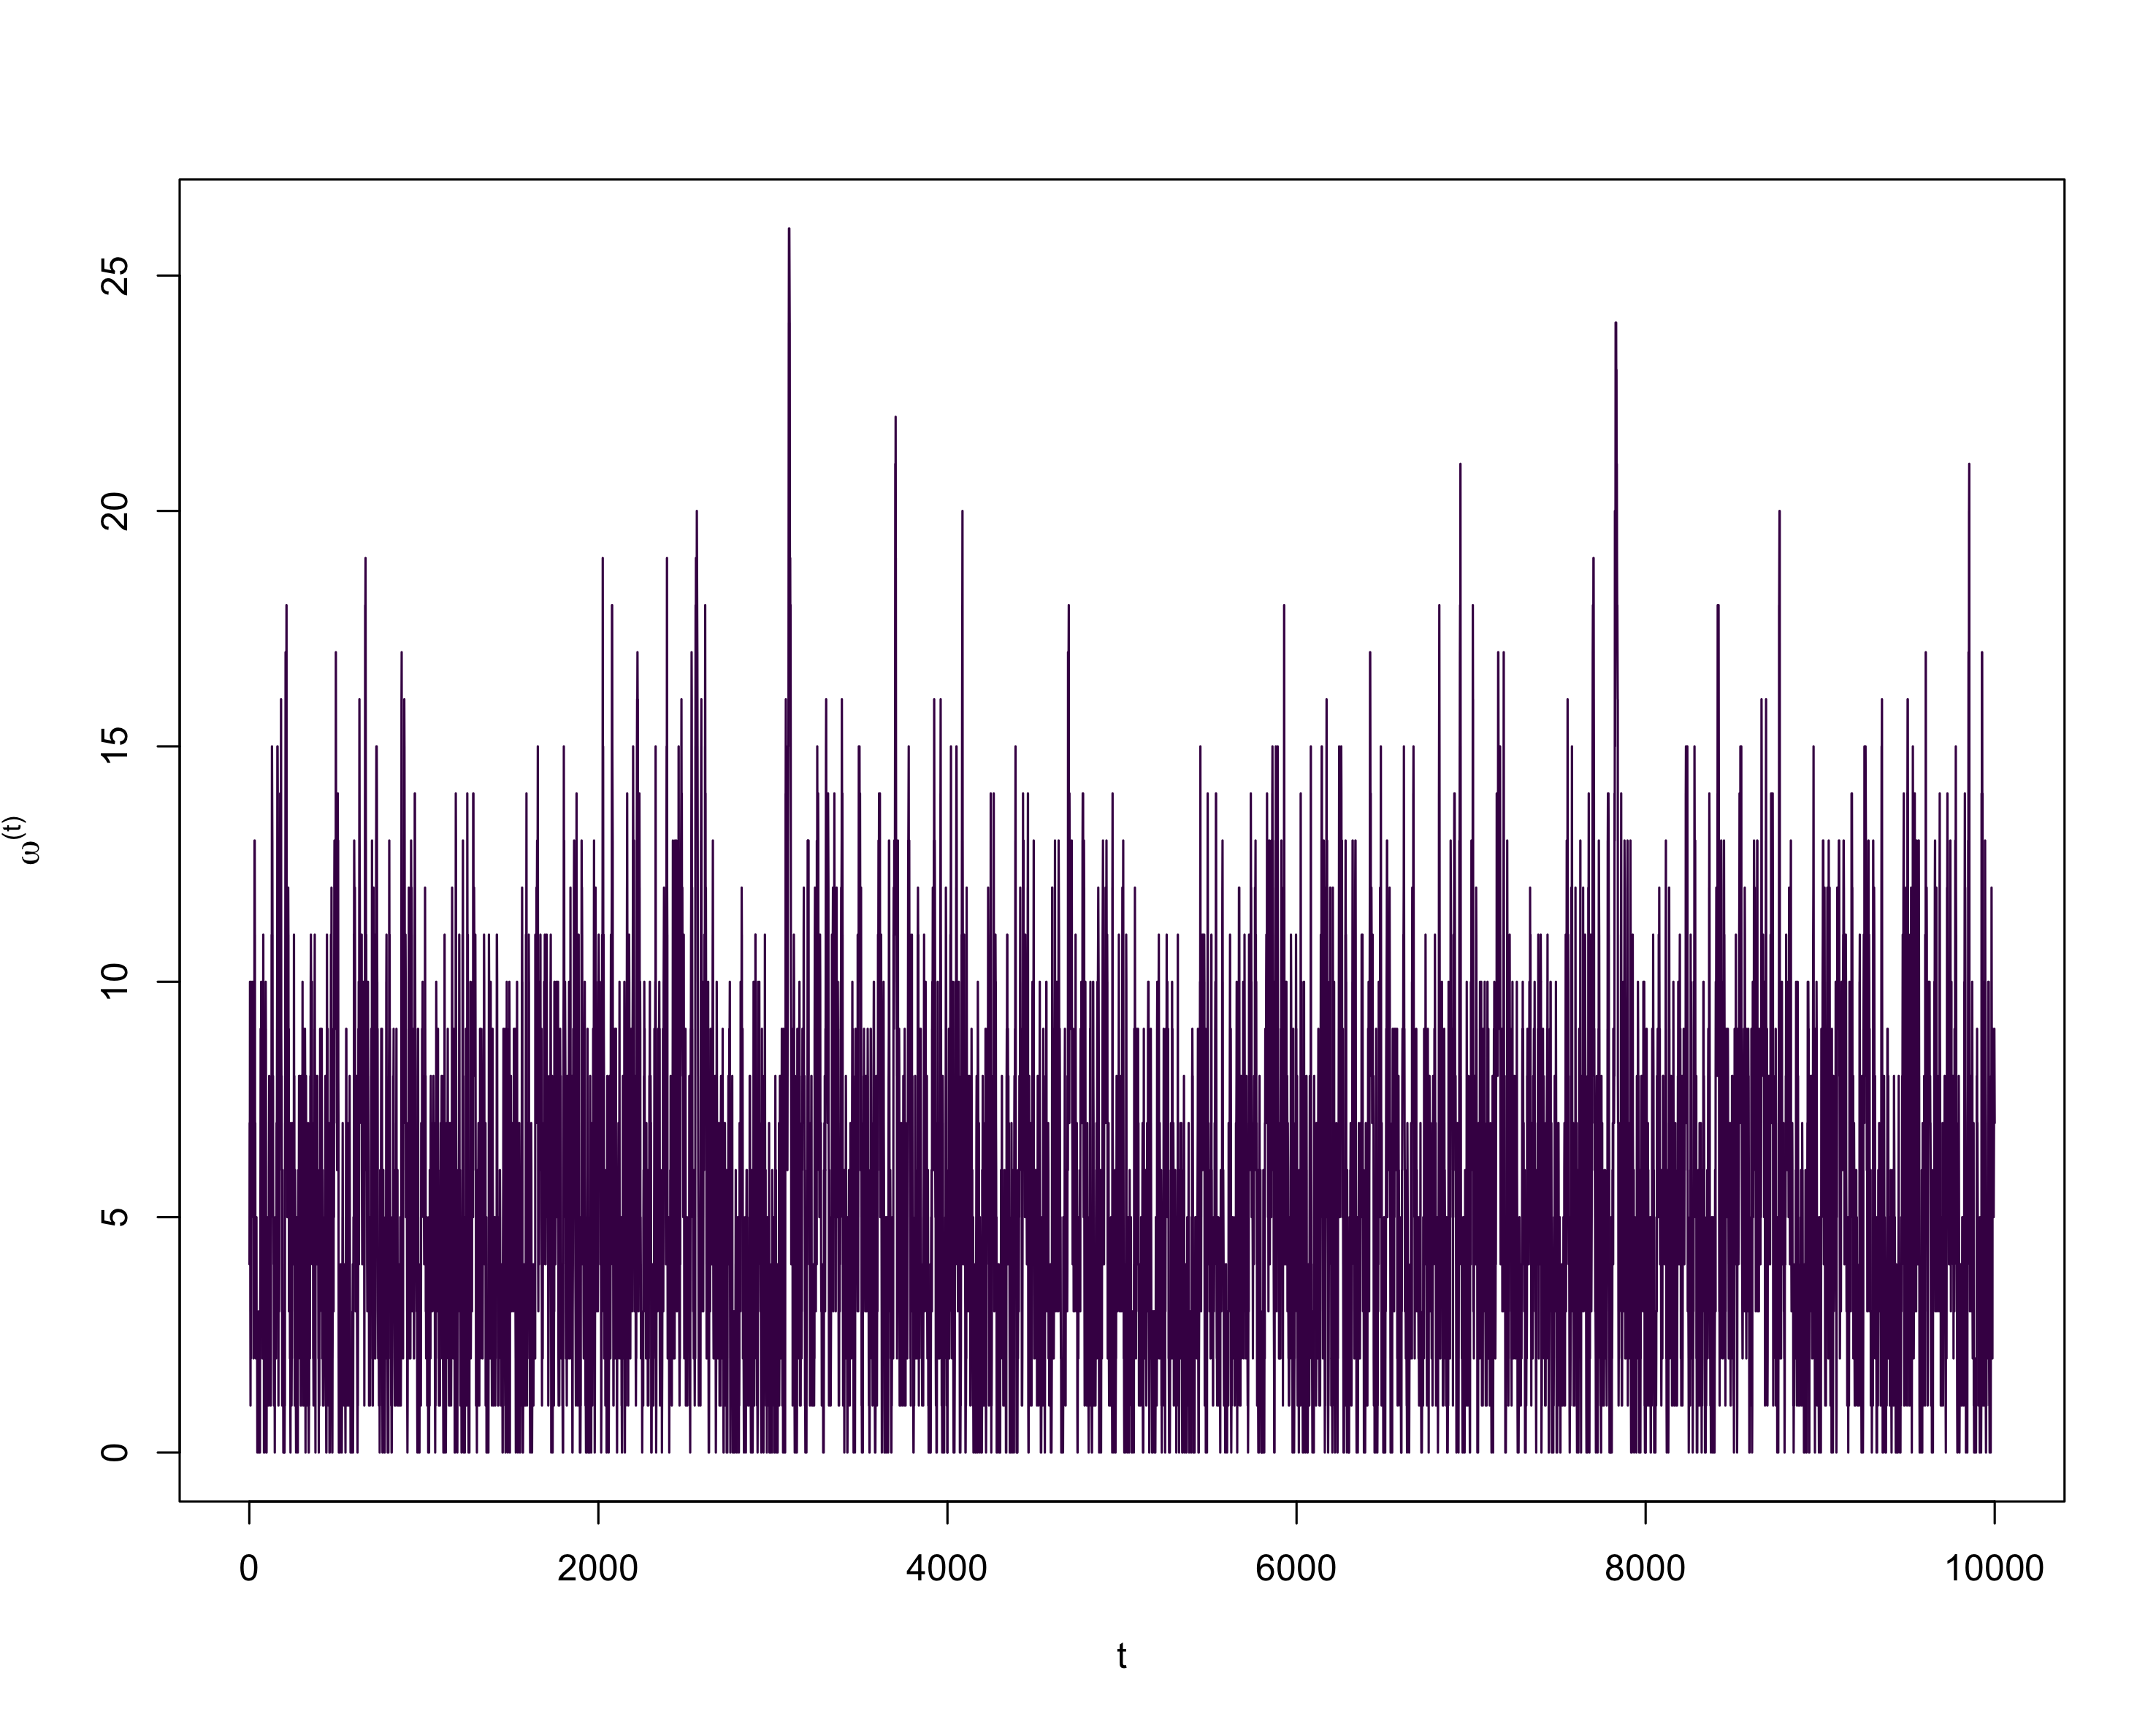
\includegraphics[width=\linewidth]{hier_chain_omega.png} 
        \caption{Proceso $\lbrace \omega_t \rbrace$} \label{fig:hier_chain_omega}
    \end{subfigure}

    \vspace{0.2cm}
    
    \begin{subfigure}[t]{0.45\textwidth}
        \centering
        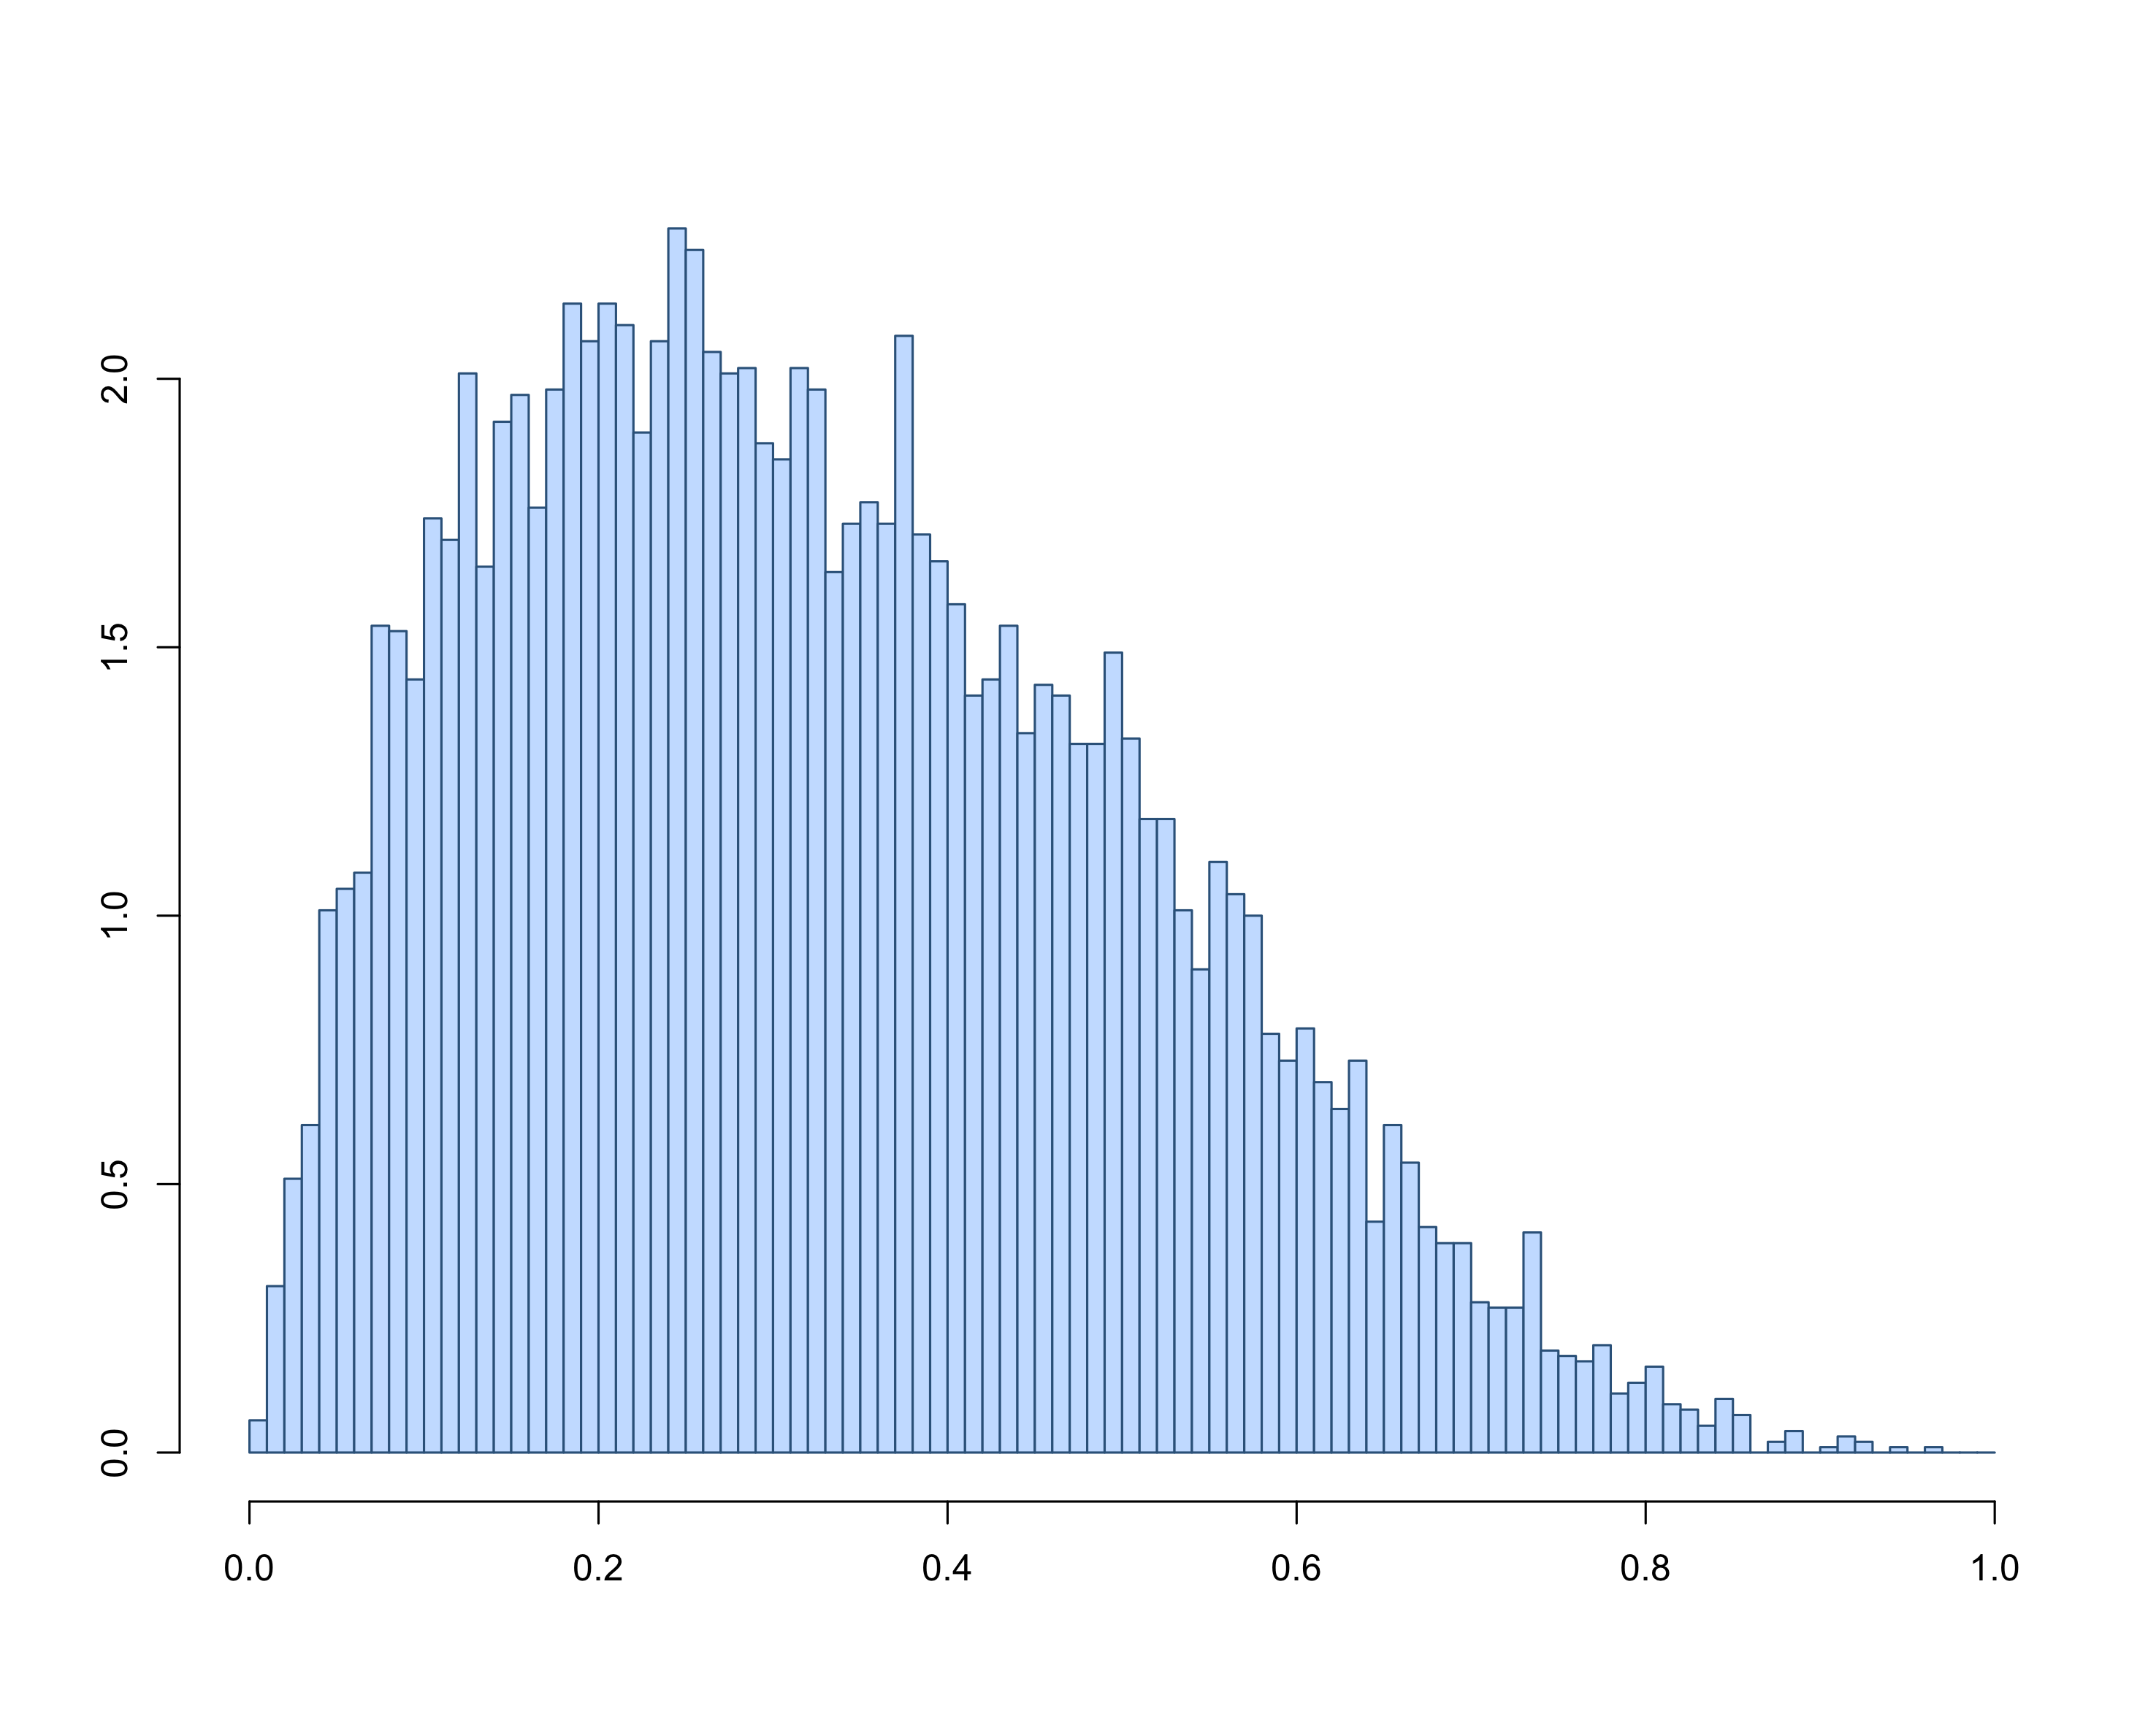
\includegraphics[width=\linewidth]{hier_hist_theta.png} 
        \caption{Distribución marginal $f_\theta$.} \label{fig:hier_hist_theta}
    \end{subfigure}
    \hfill
    \begin{subfigure}[t]{0.45\textwidth}
        \centering
        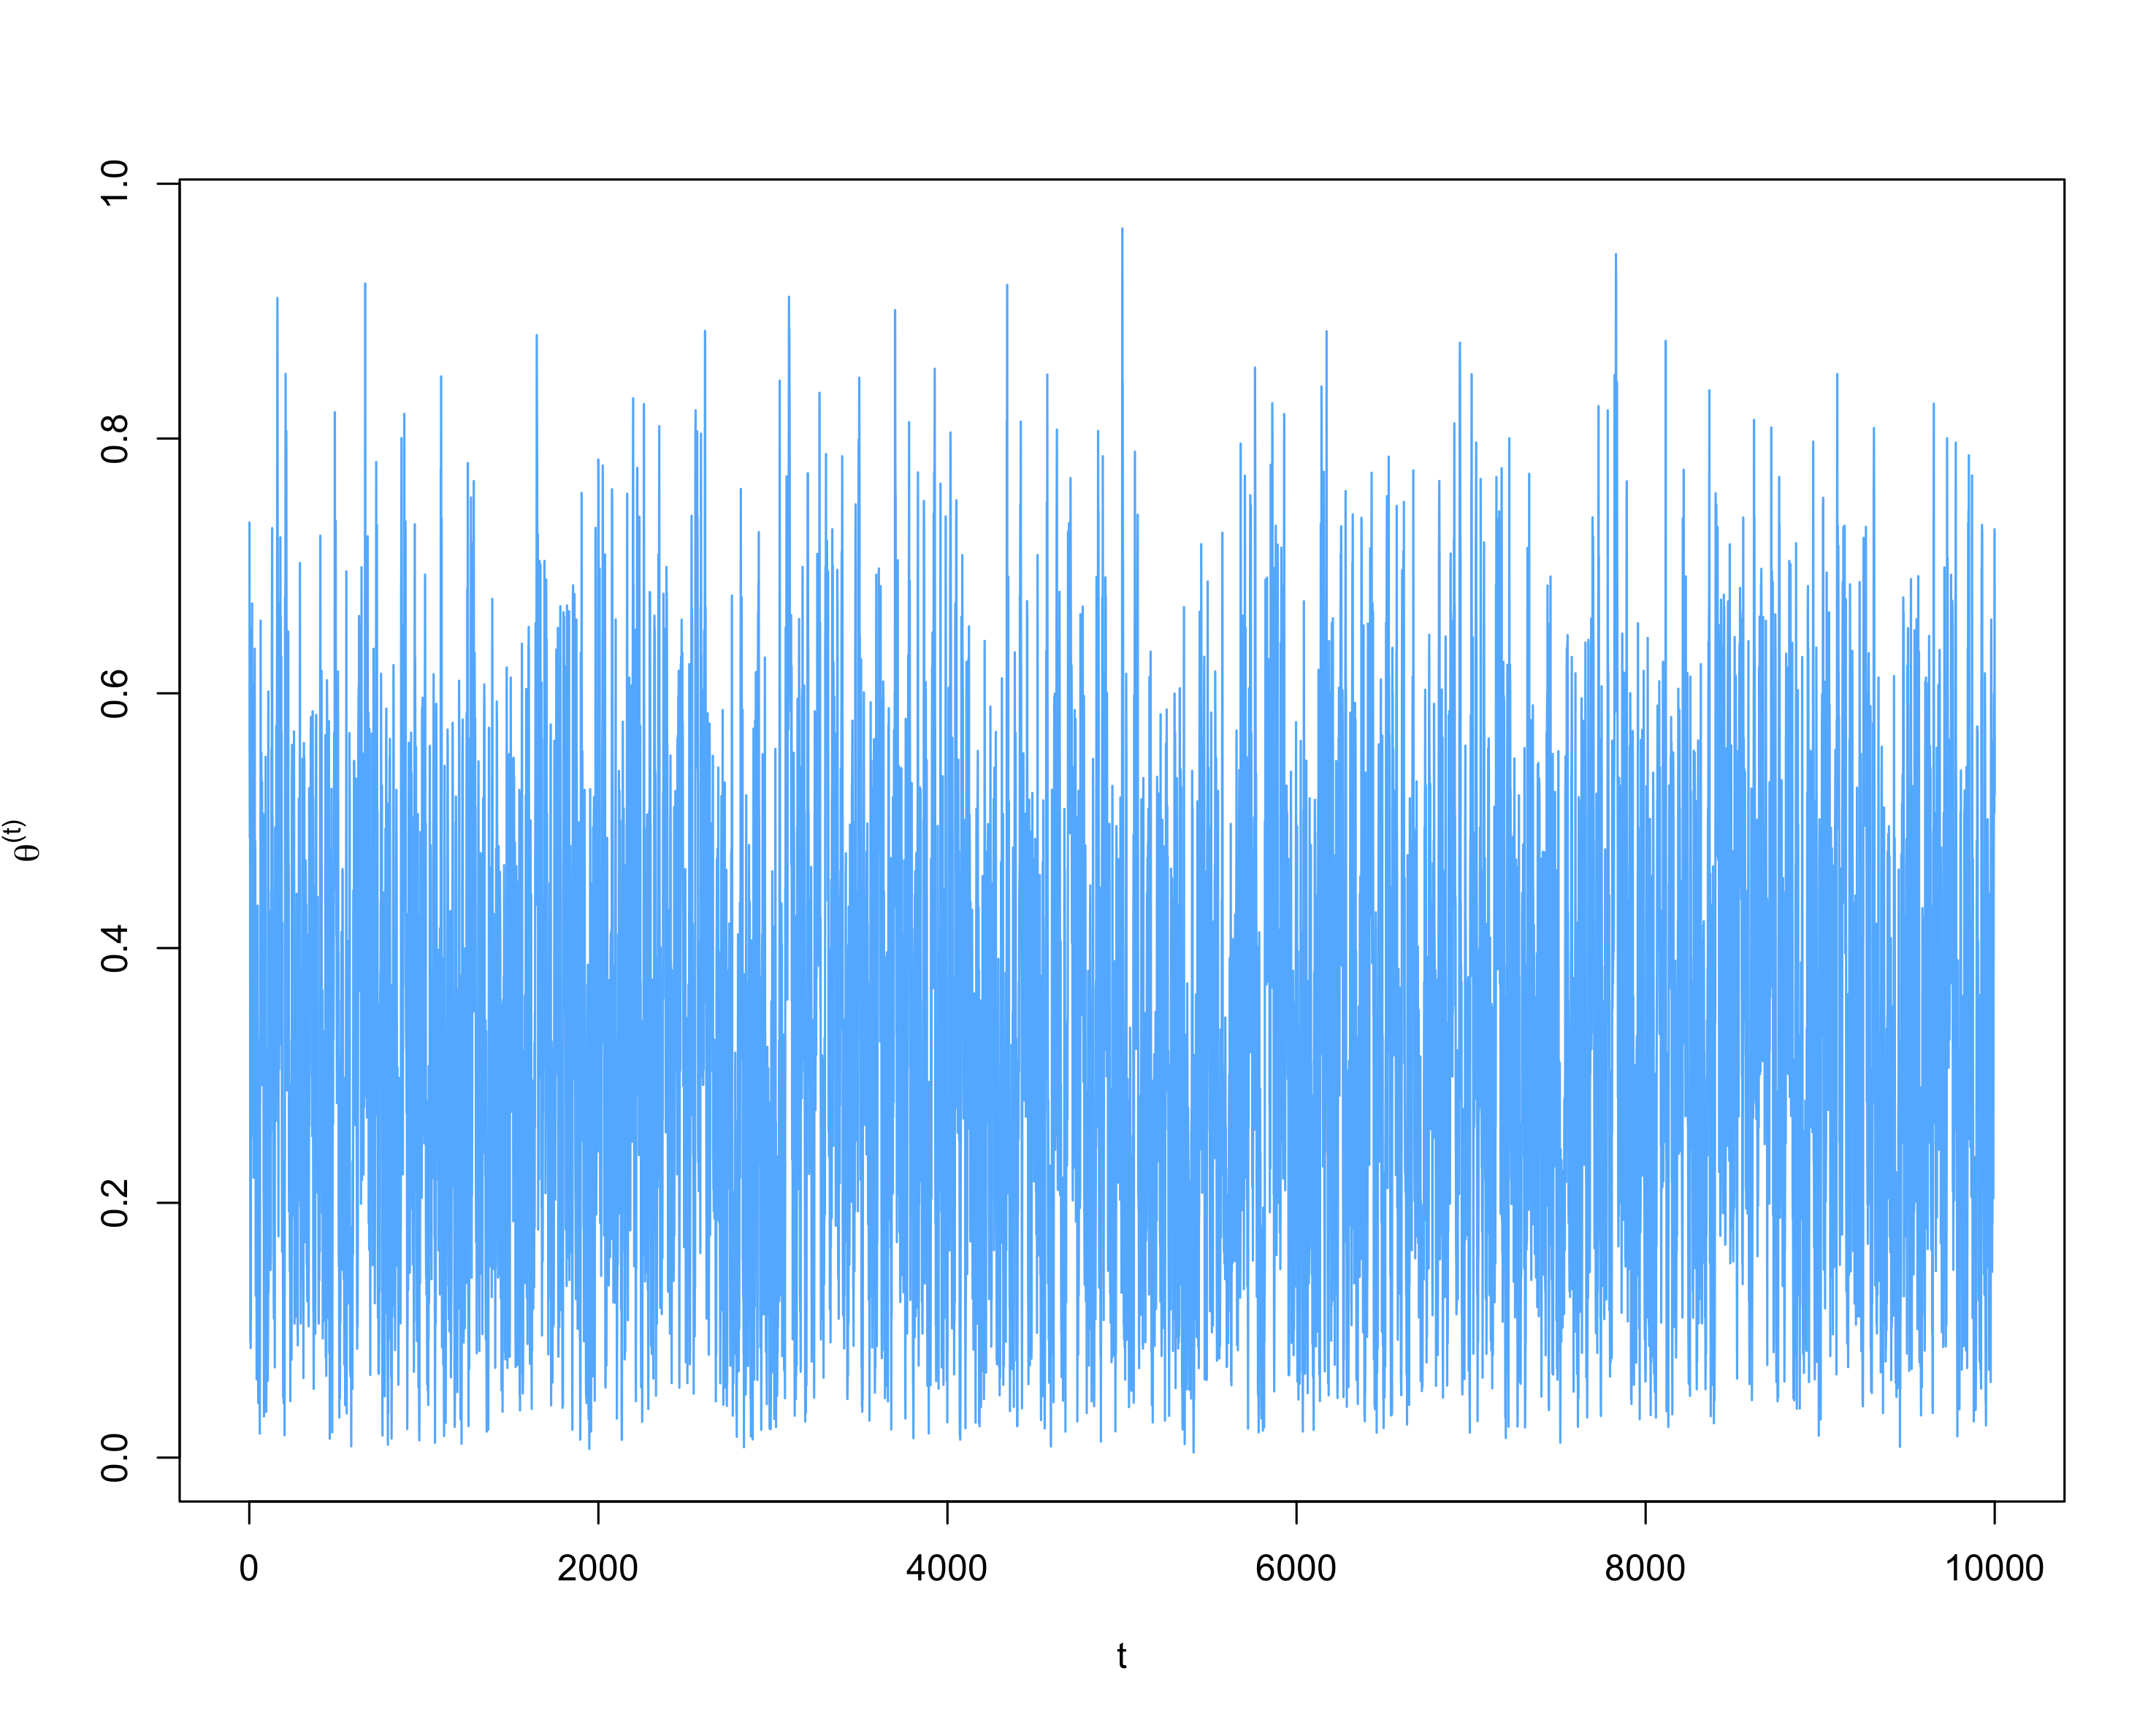
\includegraphics[width=\linewidth]{hier_chain_theta.png} 
        \caption{Proceso $\lbrace \theta_t \rbrace$} \label{fig:hier_chain_theta}
    \end{subfigure}
    
     \vspace{0.2cm}
    
    \begin{subfigure}[t]{0.45\textwidth}
        \centering
        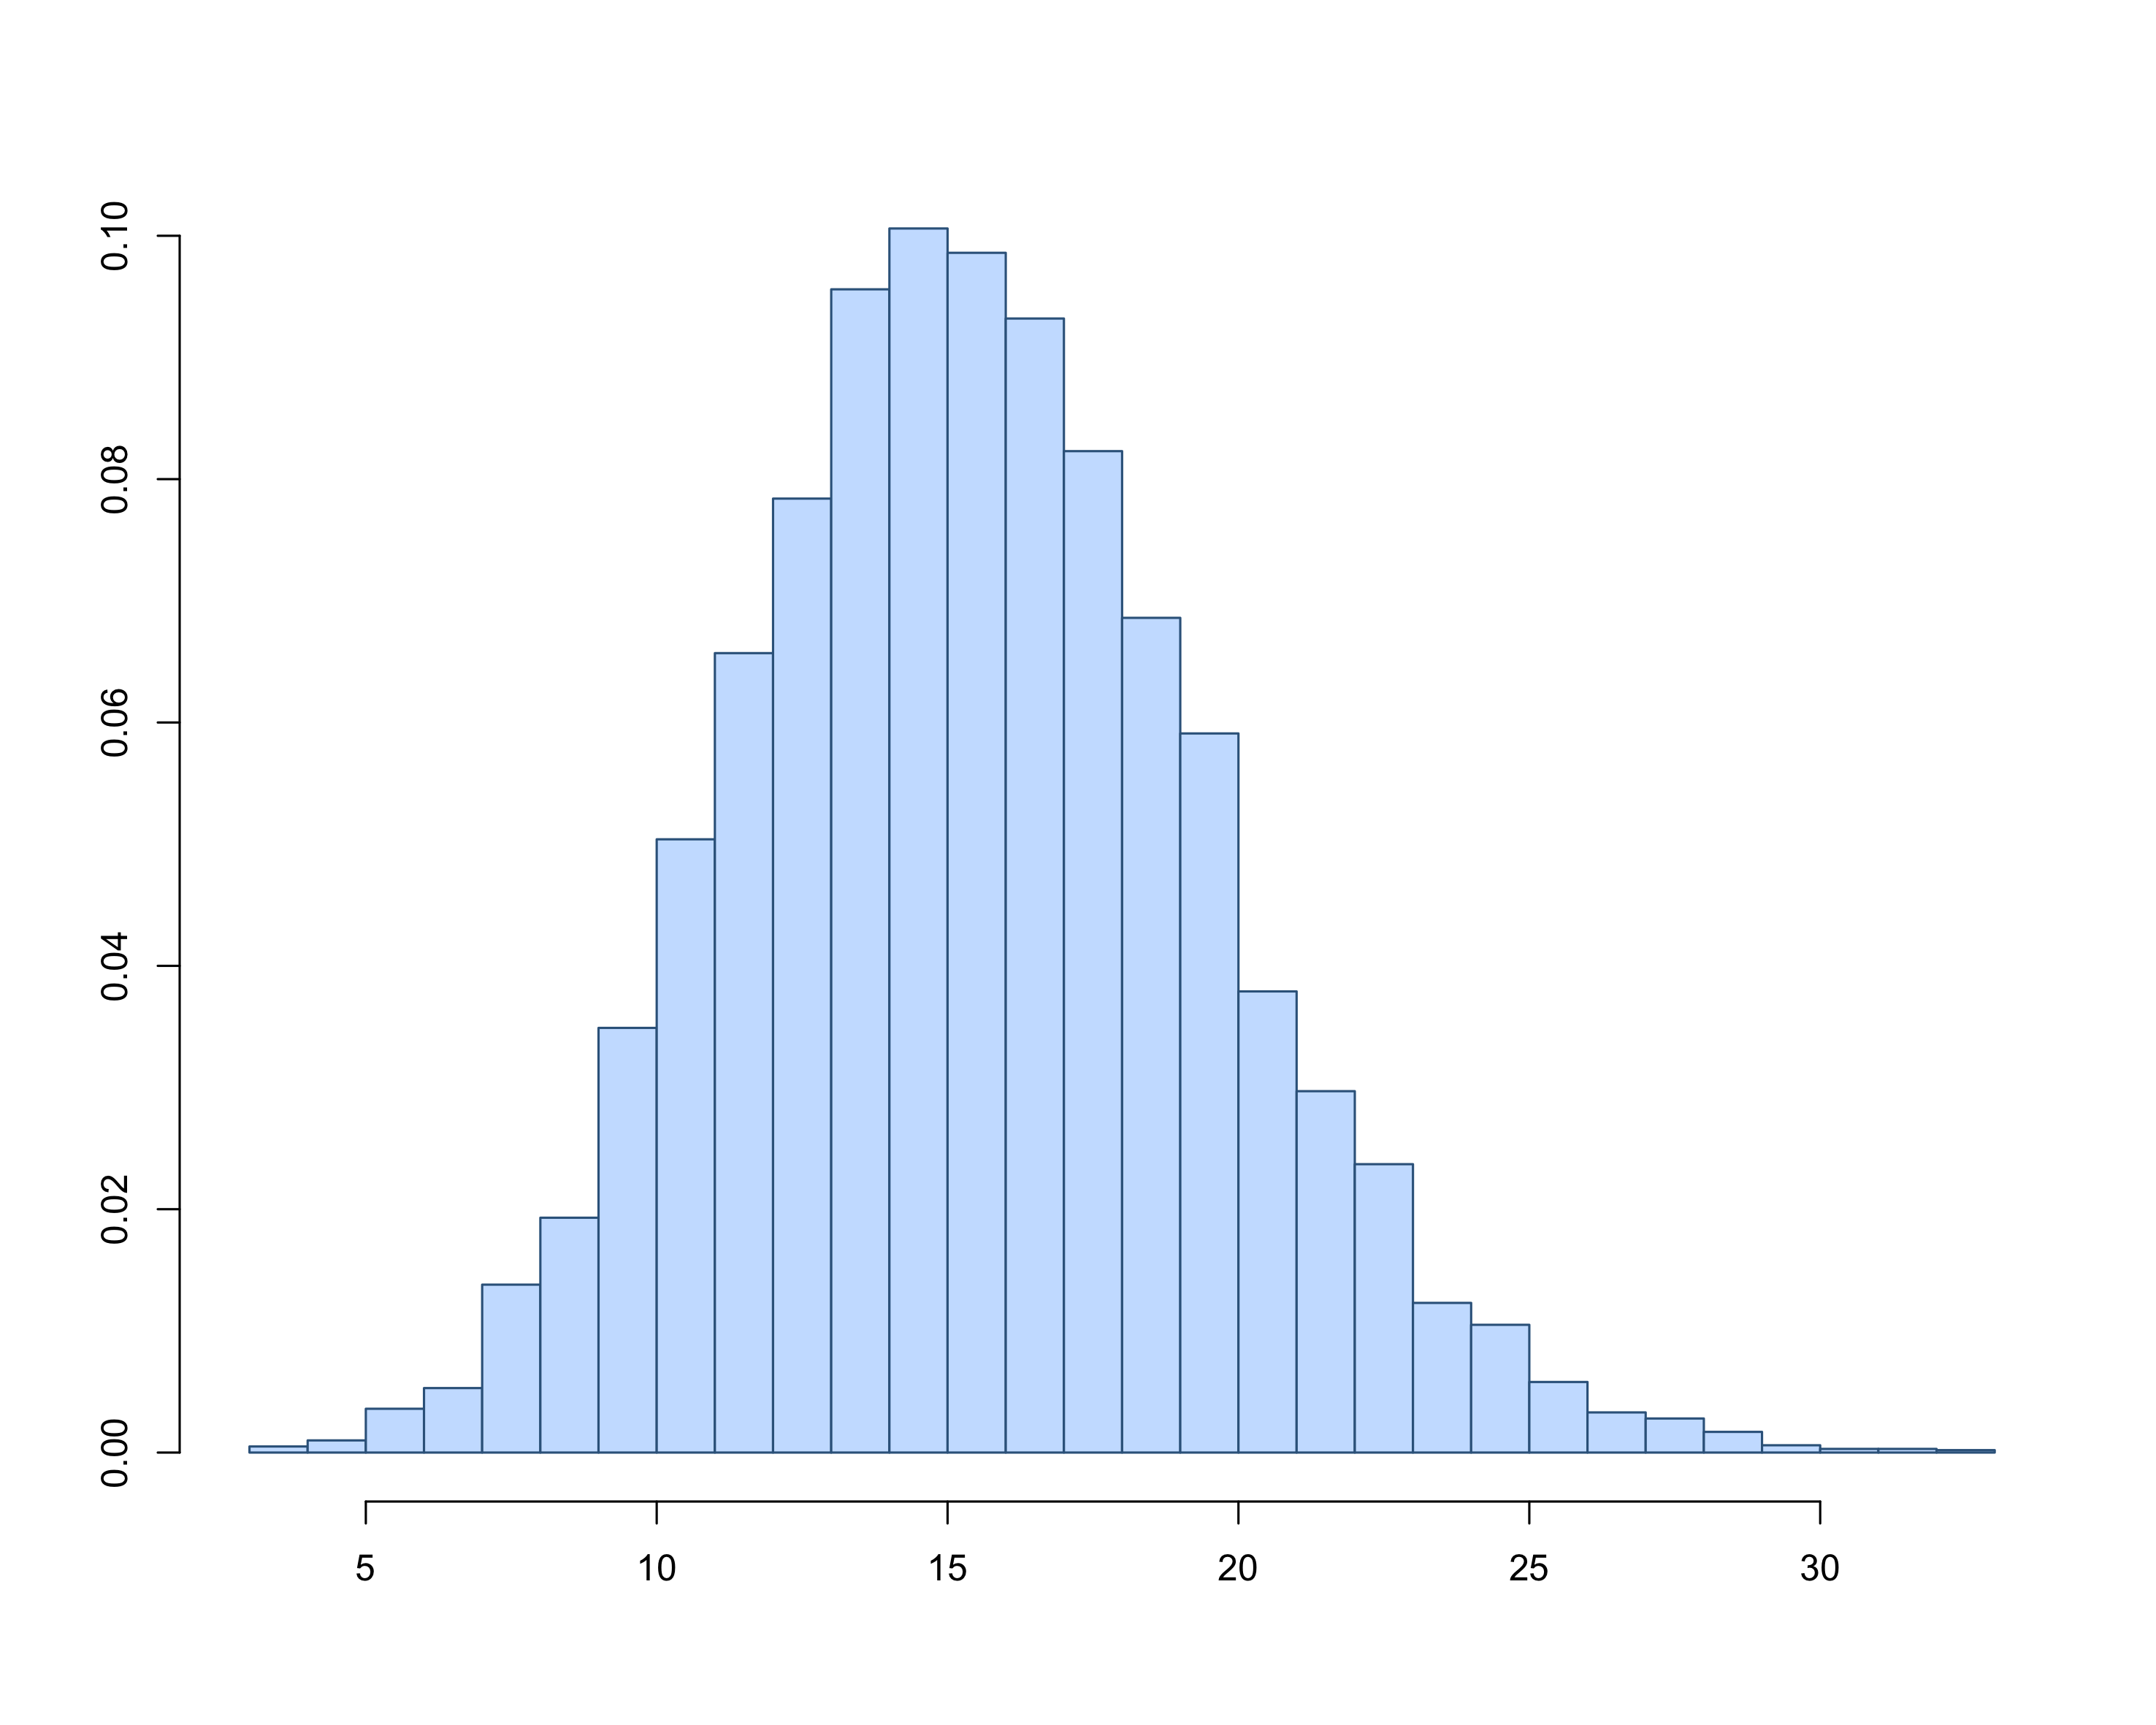
\includegraphics[width=\linewidth]{hier_hist_gamma.png} 
        \caption{Distribución marginal $f_\gamma$.} \label{fig:hier_hist_gamma}
    \end{subfigure}
    \hfill
    \begin{subfigure}[t]{0.45\textwidth}
        \centering
        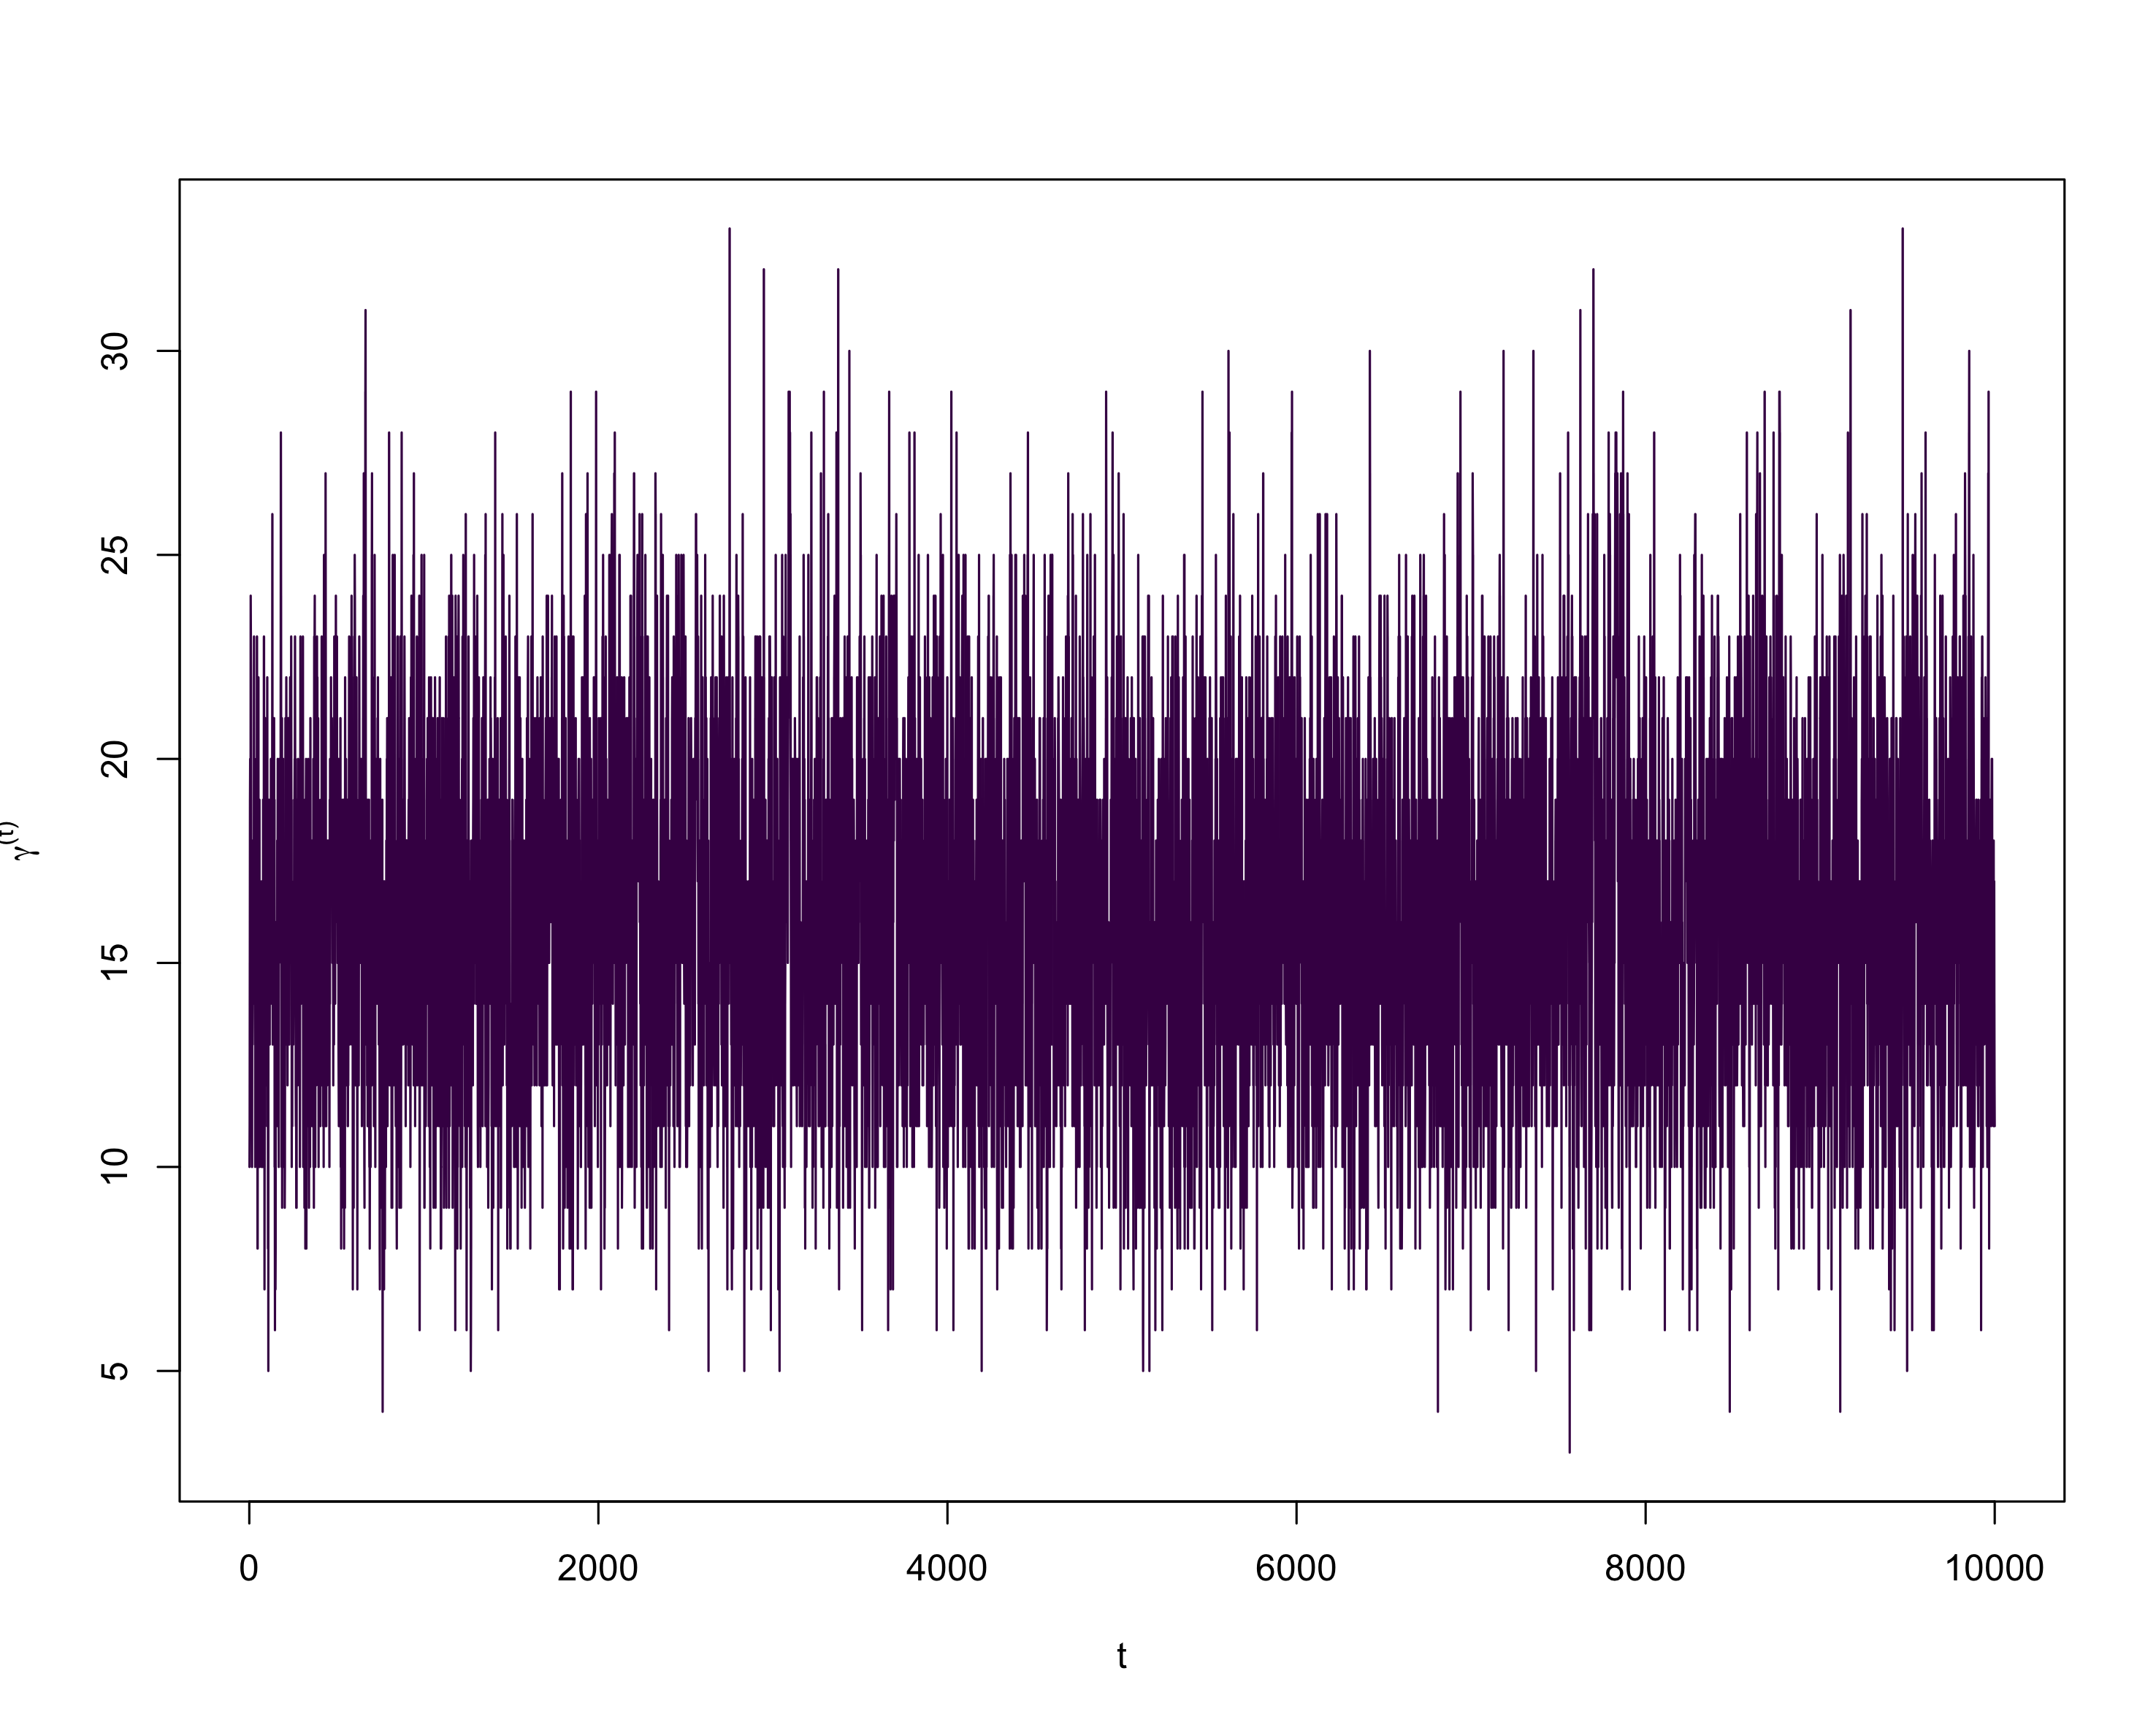
\includegraphics[width=\linewidth]{hier_chain_gamma.png} 
        \caption{Proceso $\lbrace \gamma_t \rbrace$} \label{fig:hier_chain_gamma}
    \end{subfigure}
    
    \caption{Simulaciones del modelo jerárquico utilizando el muestreador de Gibbs para tres variables con $\alpha = 2$, $\beta = 4$ y $\lambda = 16$.}
    \label{fig:gs_hier}
\end{figure}

En la figura \ref{fig:gs_hier} se presentan los histogramas de cada una de las variables, junto con el estado que visitan los procesos en cada iteración. En las \textit{gráficas de traza} presentadas en los páneles \ref{fig:hier_chain_omega}, \ref{fig:hier_chain_theta} y \ref{fig:hier_chain_gamma} se puede ver que las tres cadenas recorren todos los valores del eje de las ordenadas, lo cual sugiere que exploran el soporte de las distirbuciones de manera satisfactoria. Como se verá más adelante, ver gráficamente los procesos es útil para analizar la convergencia del algoritmo.

Antes de pasar al algoritmo de Metropolis-Hastings, es muy importante resaltar que las observaciones obtenidas con el muestreador de Gibbs \textbf{no son una muestra aleatoria}, en el sentido de que las observaciones no son independientes. Esto siginifica que las hipótesis de la ley fuerte de los grandes números (teorema \ref{grandes_numeros}) no se cumplen para estas simulaciones. Sin embargo, existe un análogo a esta ley para cadenas de Markov ergódicas, conocido como el \textit{teorema ergódico} o \textit{de ergodicidad} \citep{casella}.

\begin{theorem}[Teorema ergódico]
Si un kernel de transición $P$ produce una cadena de Markov ergódica $\lbrace X_t \rbrace$ con distribución estacionaria $f$, entonces para una función integrable $h$ se cumple que
\begin{equation}
\lim_{T \to \infty} \sum_{t = 1}^T h(X^{(t)}) = E_f[h(X)].
\end{equation}
\end{theorem}


Este resultado es de suma importancia, ya que significa que se pueden utilizar las observaciones simuladas con las cadenas de Markov para aproximar cantidades de interés con integración Monte Carlo. También resalta la importancia del análisis de convergencia para cadenas de Markov Monte Carlo, uno de los temas más estudiados para estos métodos.

\subsubsection*{Algoritmo de Metropolis-Hastings}
\label{sec:mh}

Antes de que Gelfand y Smith introdujeran el muestreador de Gibbs a la comunidad estadística, químicos y físicos ya estaban utilizando métodos de Monte Carlo en experimentos. En 1953, Nicholas Metropolis publicó un artículo en el que introdujo su algoritmo. Este artículo solamente trataba sobre el movimiento de partículas en un cuadrado y no mencionaba otras aplicaciones. En 1970, W. Keith Hastings generalizó el algoritmo de Metropolis. Sin embargo, la metodología siguió siendo ignorada en el ámbito estadístico debido a la poca disponibilidad de los recursos computacionales necesarios para explotarlo \citep{bertsch}. Fue hasta después de la publicación de Gelfand y Smith que el muestreador de Gibbs fue identificado como un caso especial del algoritmo de Metropolis-Hastings. Hastings no supo de la gran importancia que tuvo su trabajo hasta después de su retiro en 1992, más de veinte años después de publicarlo.

La idea general del algoritmo de Metropolis-Hastings es parecida a los métodos de aceptación y rechazo de la sección \ref{aceptacion}, en el sentido de que se generan observaciones de una distribución candidata y con cierta probabilidad estas observaciones son aceptadas o no. Se busca crear una cadena de Markov ergódica cuya distribución estacionaria sea la densidad de interés. A continuación se muestra cómo crear esta cadena.

Si se tiene un kernel de transición $P$ que genera una cadena de Markov ergódica con distribución estacionaria $f$, entonces el kernel y la distribución satisfacen la condición \citep{chib_mh}
$$\int_{\Omega_X} P(x, y)f(x) \ dx = f(y).$$ En el caso que interesa aquí, se conoce la distribución estacionaria $f$ (la distribución de interés) y lo que falta es encontrar el kernel de transición $P$. Para esto se busca una función auxiliar $p(x, y)$ que satisfaga la condición de reversibilidad \citep{chib_mh}
\begin{equation} \label{eq:reversibilidad}
f(x)p(x, y) = f(y)p(y, x).
\end{equation}
Los mismos autores explican cómo encontrar esta función $p$.

Supóngase que se tiene una función de densidad que genera candidatos para la transición de la cadena. Esta densidad es denotada $q(y|x)$, señalando que si el proceso se encuentra en el estado $x$, entonces la densidad genera un valor $y \sim q(y|x)$. Normalmente esta función no va a satisfacer la condición \eqref{eq:reversibilidad}, lo que significa que es más probable pasar al estado $y$ viniendo de $x$ que pasar al estado $x$ viniendo de $y$ (o al revés). Entonces se necesita ajustar la distribución candidata con una probabilidad $\alpha (x, y)$ de que el movimiento se realice. Hasta ahora se tiene que, para $x \neq y$, $$p(x, y) = q(y | x) \alpha (x, y).$$ Suponiendo que $q$ no satisface la condición de reversibilidad porque la transición $x \to y$ es más probable que la transición $y \to x$, es decir, $$f(x)q(y|x) > f(y)q(x|y),$$ por lo que $$\frac{f(y)q(x|y)}{f(x)q(y|x)} < 1,$$ se quiere entonces que la probabilidad $\alpha(y, x)$ sea lo más grande posible para compensar la baja probabilidad de la transición $y \to x$. Ya que se fija $\alpha(y, x) = 1$, se puede obtener $\alpha(x, y)$ a partir de la ecuación \eqref{eq:reversibilidad}:
\begin{align*}
f(x)p(x, y) = f(y) p(y, x) &\implies f(x) q(y|x) \alpha(x, y) = f(y) q(x|y)\alpha (y, x)\\
&\implies f(x) q(y|x) \alpha(x, y) = f(y) q(x|y)\\
&\implies \alpha(x, y) = \frac{f(y)q(x|y)}{f(x)q(y|x)} < 1.
\end{align*}
En el caso contrario en que la condición de reversibilidad no se cumpla porque el paso $y \to x$ es más probable que el paso $x \to y$, entonces se tendría que $$\frac{f(y)q(x|y)}{f(x)q(y|x)} > 1$$ y se fija $\alpha(x, y) = 1$. Por lo tanto, si se define
\begin{equation}
\label{eq:prob_transicion}
\alpha(x, y) = \min \lbrace \rho(x, y), 1 \rbrace,
\end{equation}
donde $\rho(x, y)$ es la razón de Hastings definida como $$\rho(x, y) = \frac{f(y)q(x|y)}{f(x)q(y|x)},$$ se tiene que $p(x, y)$ satisface la condición \eqref{eq:reversibilidad} y se obtiene el kernel de transición buscado. Este kernel es de la siguiente forma. Si la cadena se encuentra en el estado $x^{(t)}$, se genera una observación candidata $y \sim q(y|x^{(t)})$ y se hace
\begin{equation}
\label{eq:mh}
X^{(t+1)} = \begin{cases} 
      y & \text{con probabilidad } \alpha(x^{(t)}, y),\\
      x^{(t)} & \text{con probabilidad } 1-\alpha(x^{(t)}, y).
   \end{cases}
\end{equation}

Es importante notar que, en teoría, este algoritmo funciona para cualquier distribución candidata $q$, siempre y cuando esta densidad explore todo el soporte de la densidad de interés. Esto significa que no se necesita satisfacer la condición del método de aceptación y rechazo de encontrar una cota $M$ para el cociente de las densidades. Sin embargo, en la práctica la selección de $q$ va a impactar de manera importante la efectividad de las simulaciones, por lo que a continuación se estudian algunas maneras de elegir esta distribución candidata.

Una manera de elegir la distribución candidata es hacerla independiente del valor de la cadena $x^{(t)}$, es decir, $q(y|x) = g(y)$. De esta manera, la razón de Hastings se simplifica a $$\rho (x, y) = \frac{f(y)g(x)}{f(x)g(y)}.$$ Sin embargo, \citet{casella} señalan que este tipo de propuestas son imprácticas debido a la dificultad de crear propuestas adecuadas en algunos contextos. Los mismos autores sugieren explorar vecindades del valor de la cadena en la iteración anterior para ir descubriendo paso a paso las propiedades de la distribución objetivo.

Una manera de explorar estas vecindades es utilizando caminatas aleatorias de la forma $y = x^{(t)} + \epsilon$. Si la distribución de $\epsilon$ es simétrica, esto es que $f_{\epsilon} = f_{-\epsilon}$, entonces se cumple que $q(y|x) = q(x|y)$ y la razón de Hastings es simplemente $$\rho (x, y) = \frac{f(y)}{f(x)}.$$ El caso de estas propuestas simétricas fue el estudiado originalmente por Metropolis en 1953 \citep{gelman}. A veces se utiliza el nombre de algoritmo de Metropolis para indicar este tipo de distribuciones candidatas. Nótese que si la caminata aleatoria no es simétrica, entonces se debe incorporar el cociente de la densidad candidata a la razón de Hastings.

Ya que se introdujeron las propiedades del algoritmo de Metropolis-Hastings, se explica ahora por qué el muestreador de Gibbs es un caso especial de éste. Imagínese el lector que la iteración $t$ del algoritmo de Metropolis-Hastings es una serie de $p$ pasos, donde cada uno corresponde a un subvector $\theta_i$ de $\theta$. El $i$-ésimo paso de la iteración $t$ solamente mueve el subvector $\theta_i$ utilizando la densidad condicional de $\theta_i | \theta^{(t-1)}_{-i}$ \citep{gelman}:
$$q_i(\theta^* | \theta^{(t-1)}) = \begin{cases}
f_{\theta_i | \theta_{-i}^{(t-1)}} (\theta^*_{i}) & \text{si } \theta^*_{-i} = \theta^{(t-1)}_{-i},\\
0 & \text{en otro caso.} \end{cases}$$ De esta forma, la razón de Hastings es
\begin{align*}
\rho(\theta^{(t-1)}, \theta^*) &= \frac{f(\theta^*) \ q_i(\theta^{(t-1)}|\theta^*)}{f(\theta^{(t-1)}) \ q_i(\theta^*|\theta^{(t-1)})}\\
&= \frac{f(\theta^*) \ f_{\theta_i|\theta_{-i}^{(t-1)}}(\theta^{(t-1)})}{f(\theta^{(t-1)}) \ f_{\theta_i|\theta_{-i}^{(t-1)}}(\theta^*)}\\
&= \frac{f(\theta^*)f(\theta^{(t-1)})}{f(\theta^{(t-1)})f(\theta^*)}\\
&= 1,
\end{align*}
donde $$\frac{f_{\theta_i|\theta_{-i}^{(t-1)}}(\theta^{(t-1)})}{f_{\theta_i|\theta_{-i}^{(t-1)}}(\theta^*)} = \frac{f(\theta^{(t-1)})}{f(\theta^*)}$$ porque $\theta_{-i}^* = \theta_{-i}^{(t-1)}$. Esto prueba que el muestreador de Gibbs es un caso especial del algoritmo de Metropolis-Hastings. También es interesante resaltar que el hecho de que  $\rho(\theta^{(t-1)}, \theta^*) = 1$ en este caso, explica por qué la observación propuesta siempre es aceptada en el muestreador de Gibbs.

Ahora se presenta un ejemplo de cómo utilizar el algoritmo de Metropolis-Hastings. La distribución objetivo es una $t-Student$ con 5 grados de libertad, denotada $t_{(5)}$ y se comparan tres distribuciones candidatas diferentes:
\begin{enumerate}
\item $q_1$ independiente, $q_1(y|x) = g(y) \sim \mathcal{N}(0, 1).$
\item Caminata aleatoria simétrica $q_2(y|x) \sim \mathcal{N}(x, 1).$
\item Caminata aleatoria simétrica $q_3(y|x) \sim U(x - 1, x + 1).$
\end{enumerate}
Se denota como $\lbrace X_t^i \rbrace$ a la cadena generada con la distribución candidata $q_i$.

\begin{figure}[!p]
    \centering
    \begin{subfigure}[t]{0.45\textwidth}
        \centering
        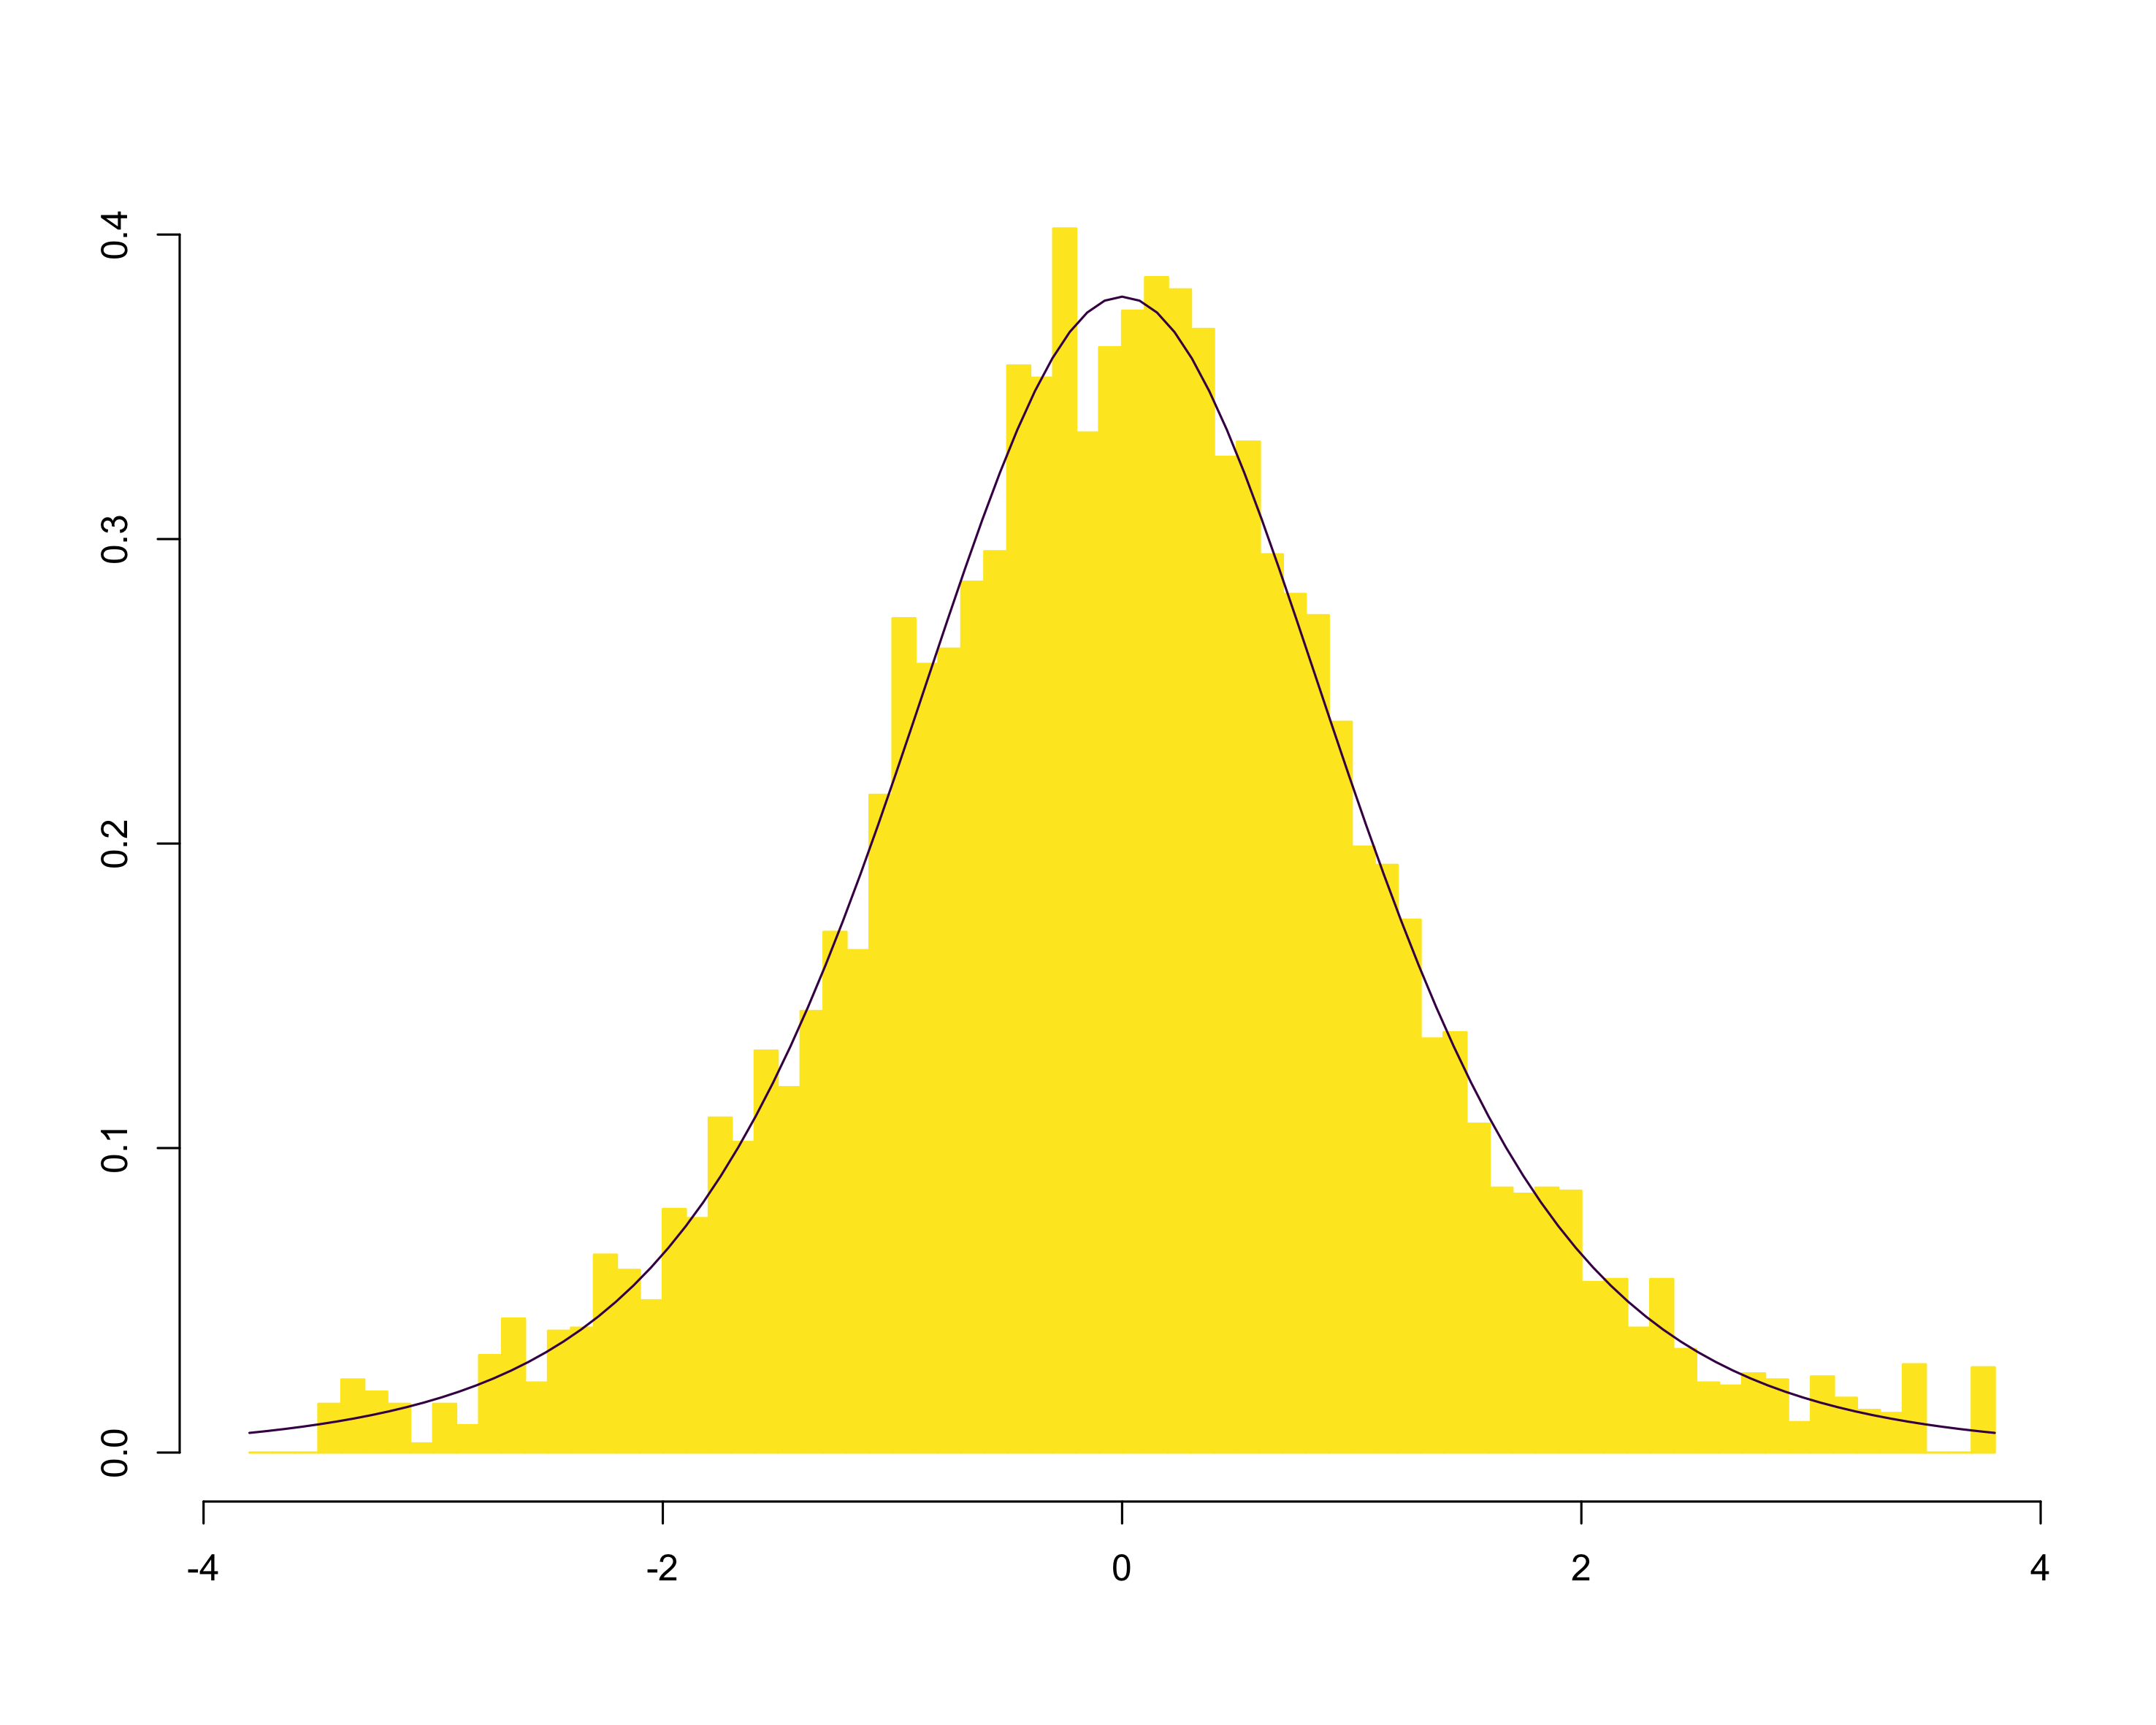
\includegraphics[width=\linewidth]{mh_hist_x1.png} 
        \caption{Histograma de $f \sim t_{(5)}$ con propuestas $q_1$} \label{fig:mh_hist_x1}
    \end{subfigure}
    \hfill
    \begin{subfigure}[t]{0.45\textwidth}
        \centering
        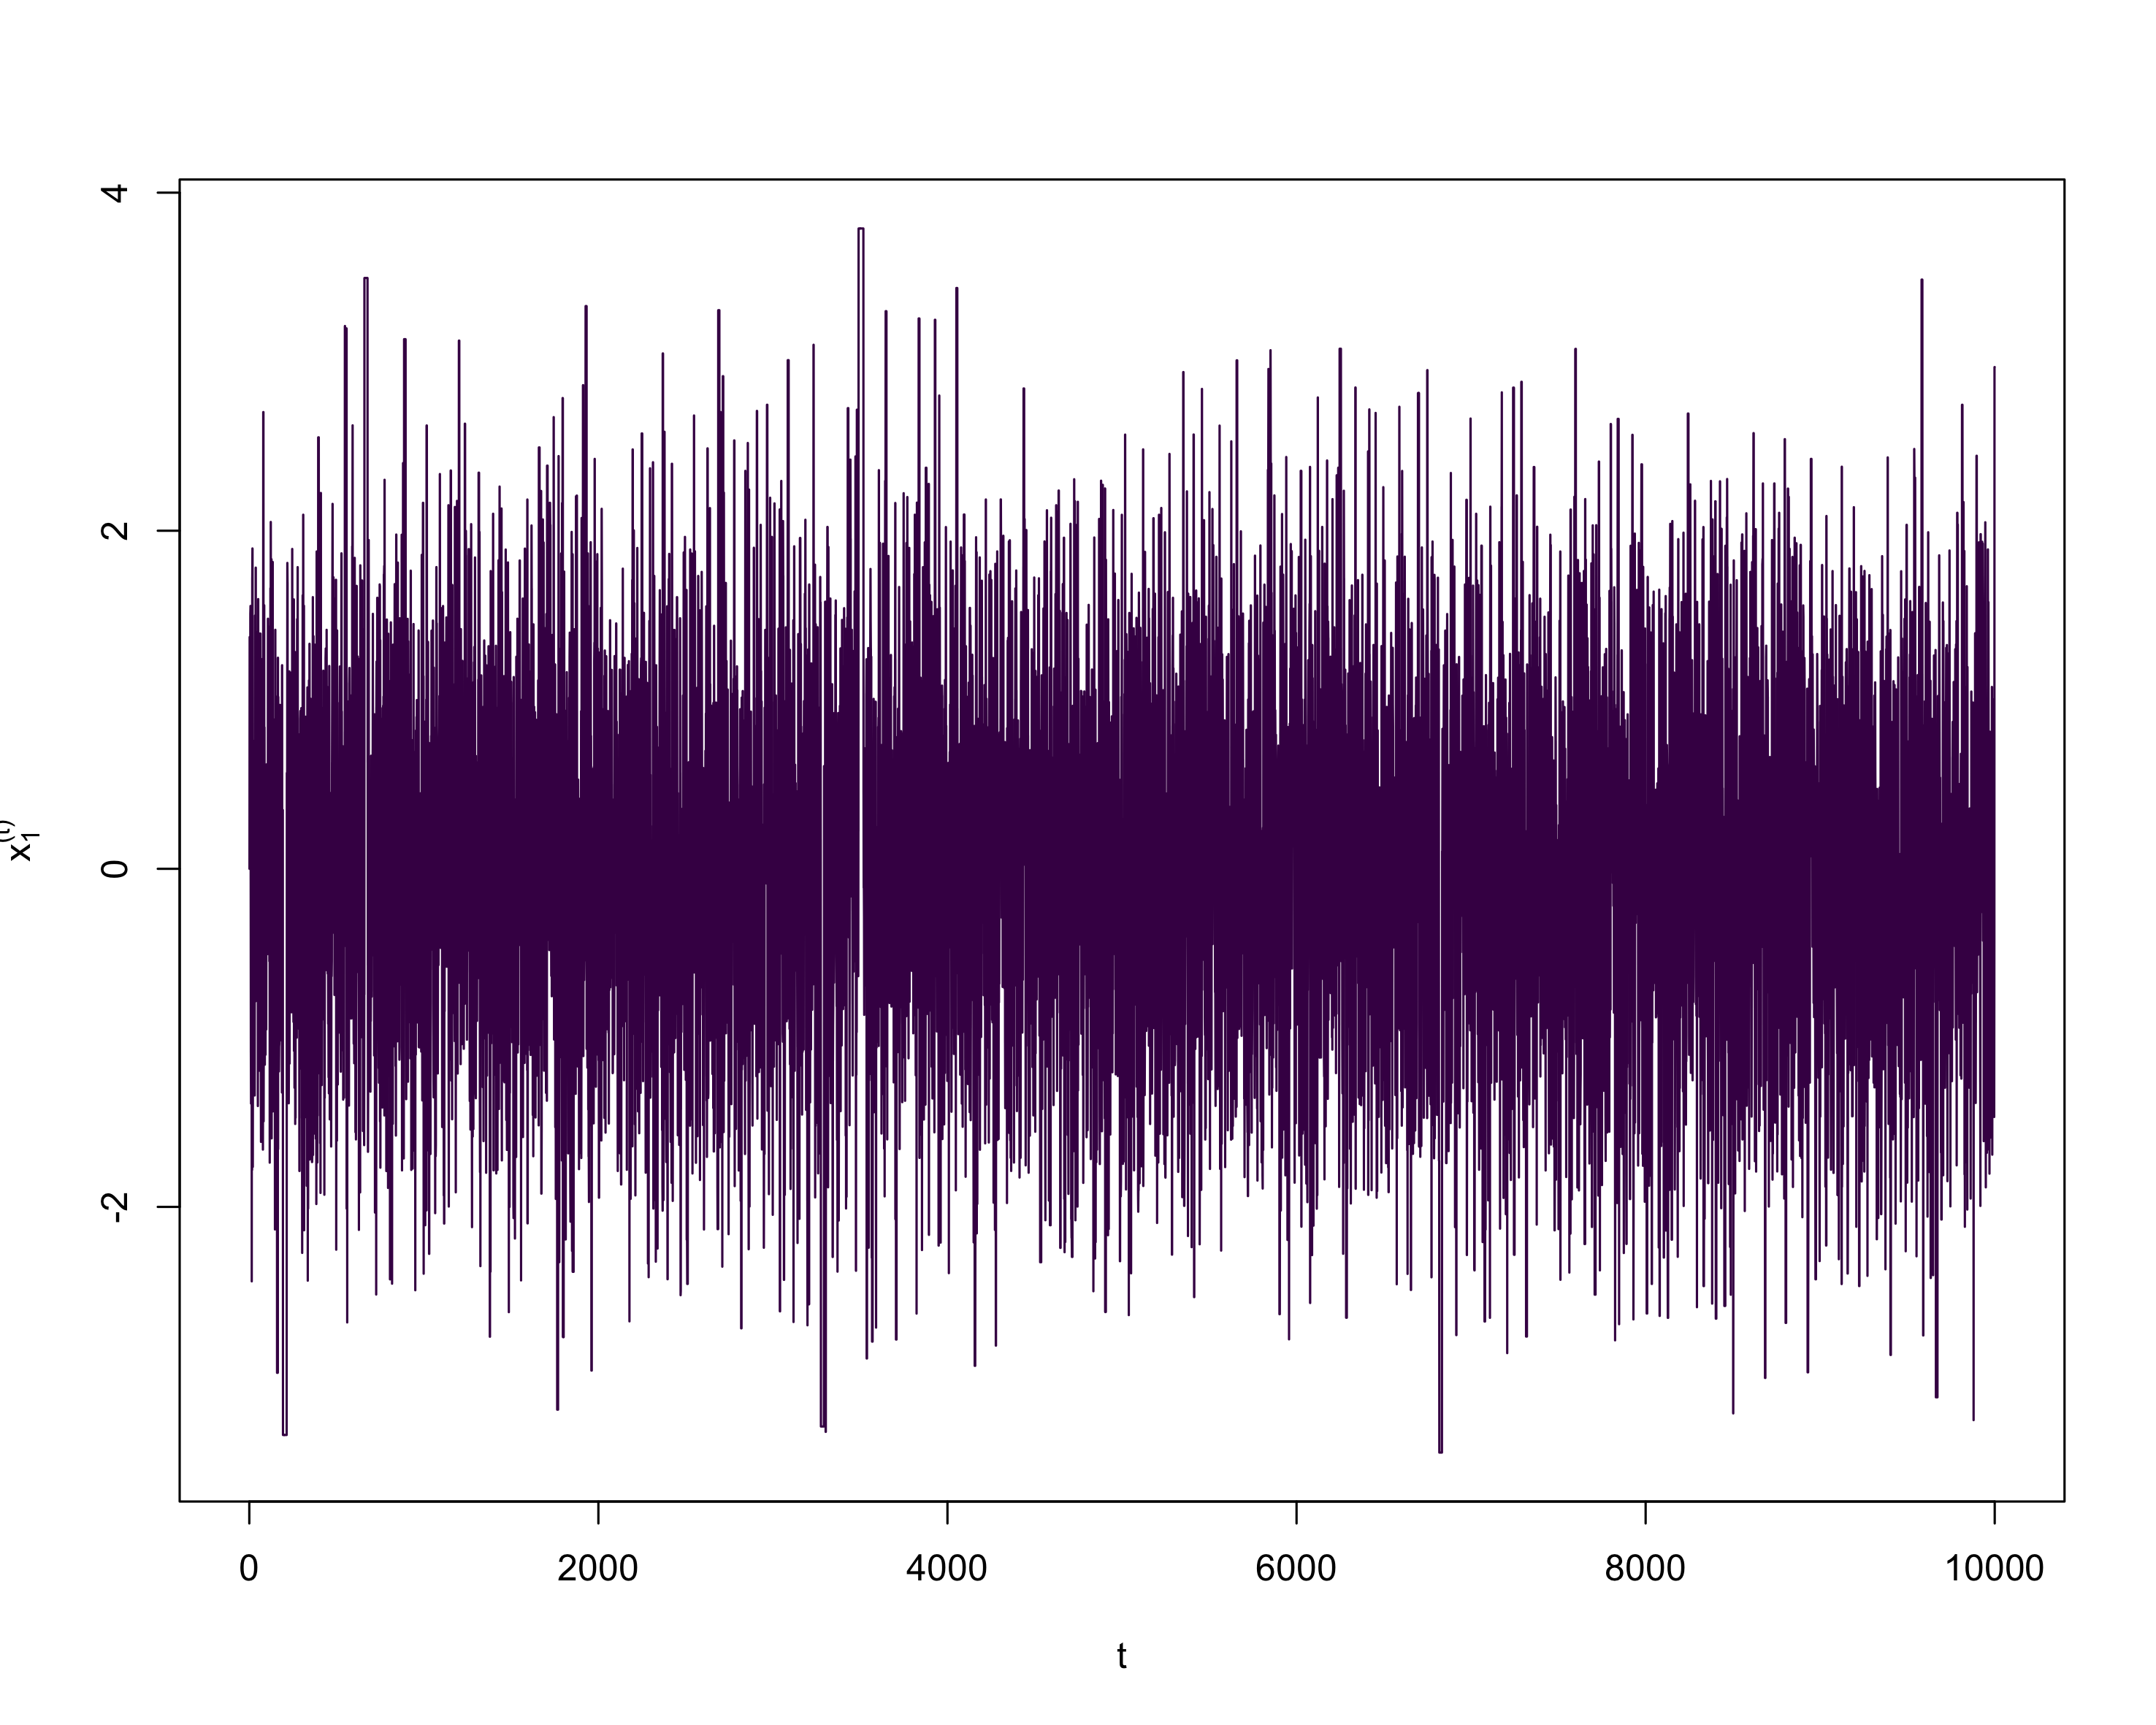
\includegraphics[width=\linewidth]{mh_chain_x1.png} 
        \caption{Proceso $\lbrace X_t^1 \rbrace$} \label{fig:mh_chain_x1}
    \end{subfigure}

    \vspace{0.2cm}
    
    \begin{subfigure}[t]{0.45\textwidth}
        \centering
        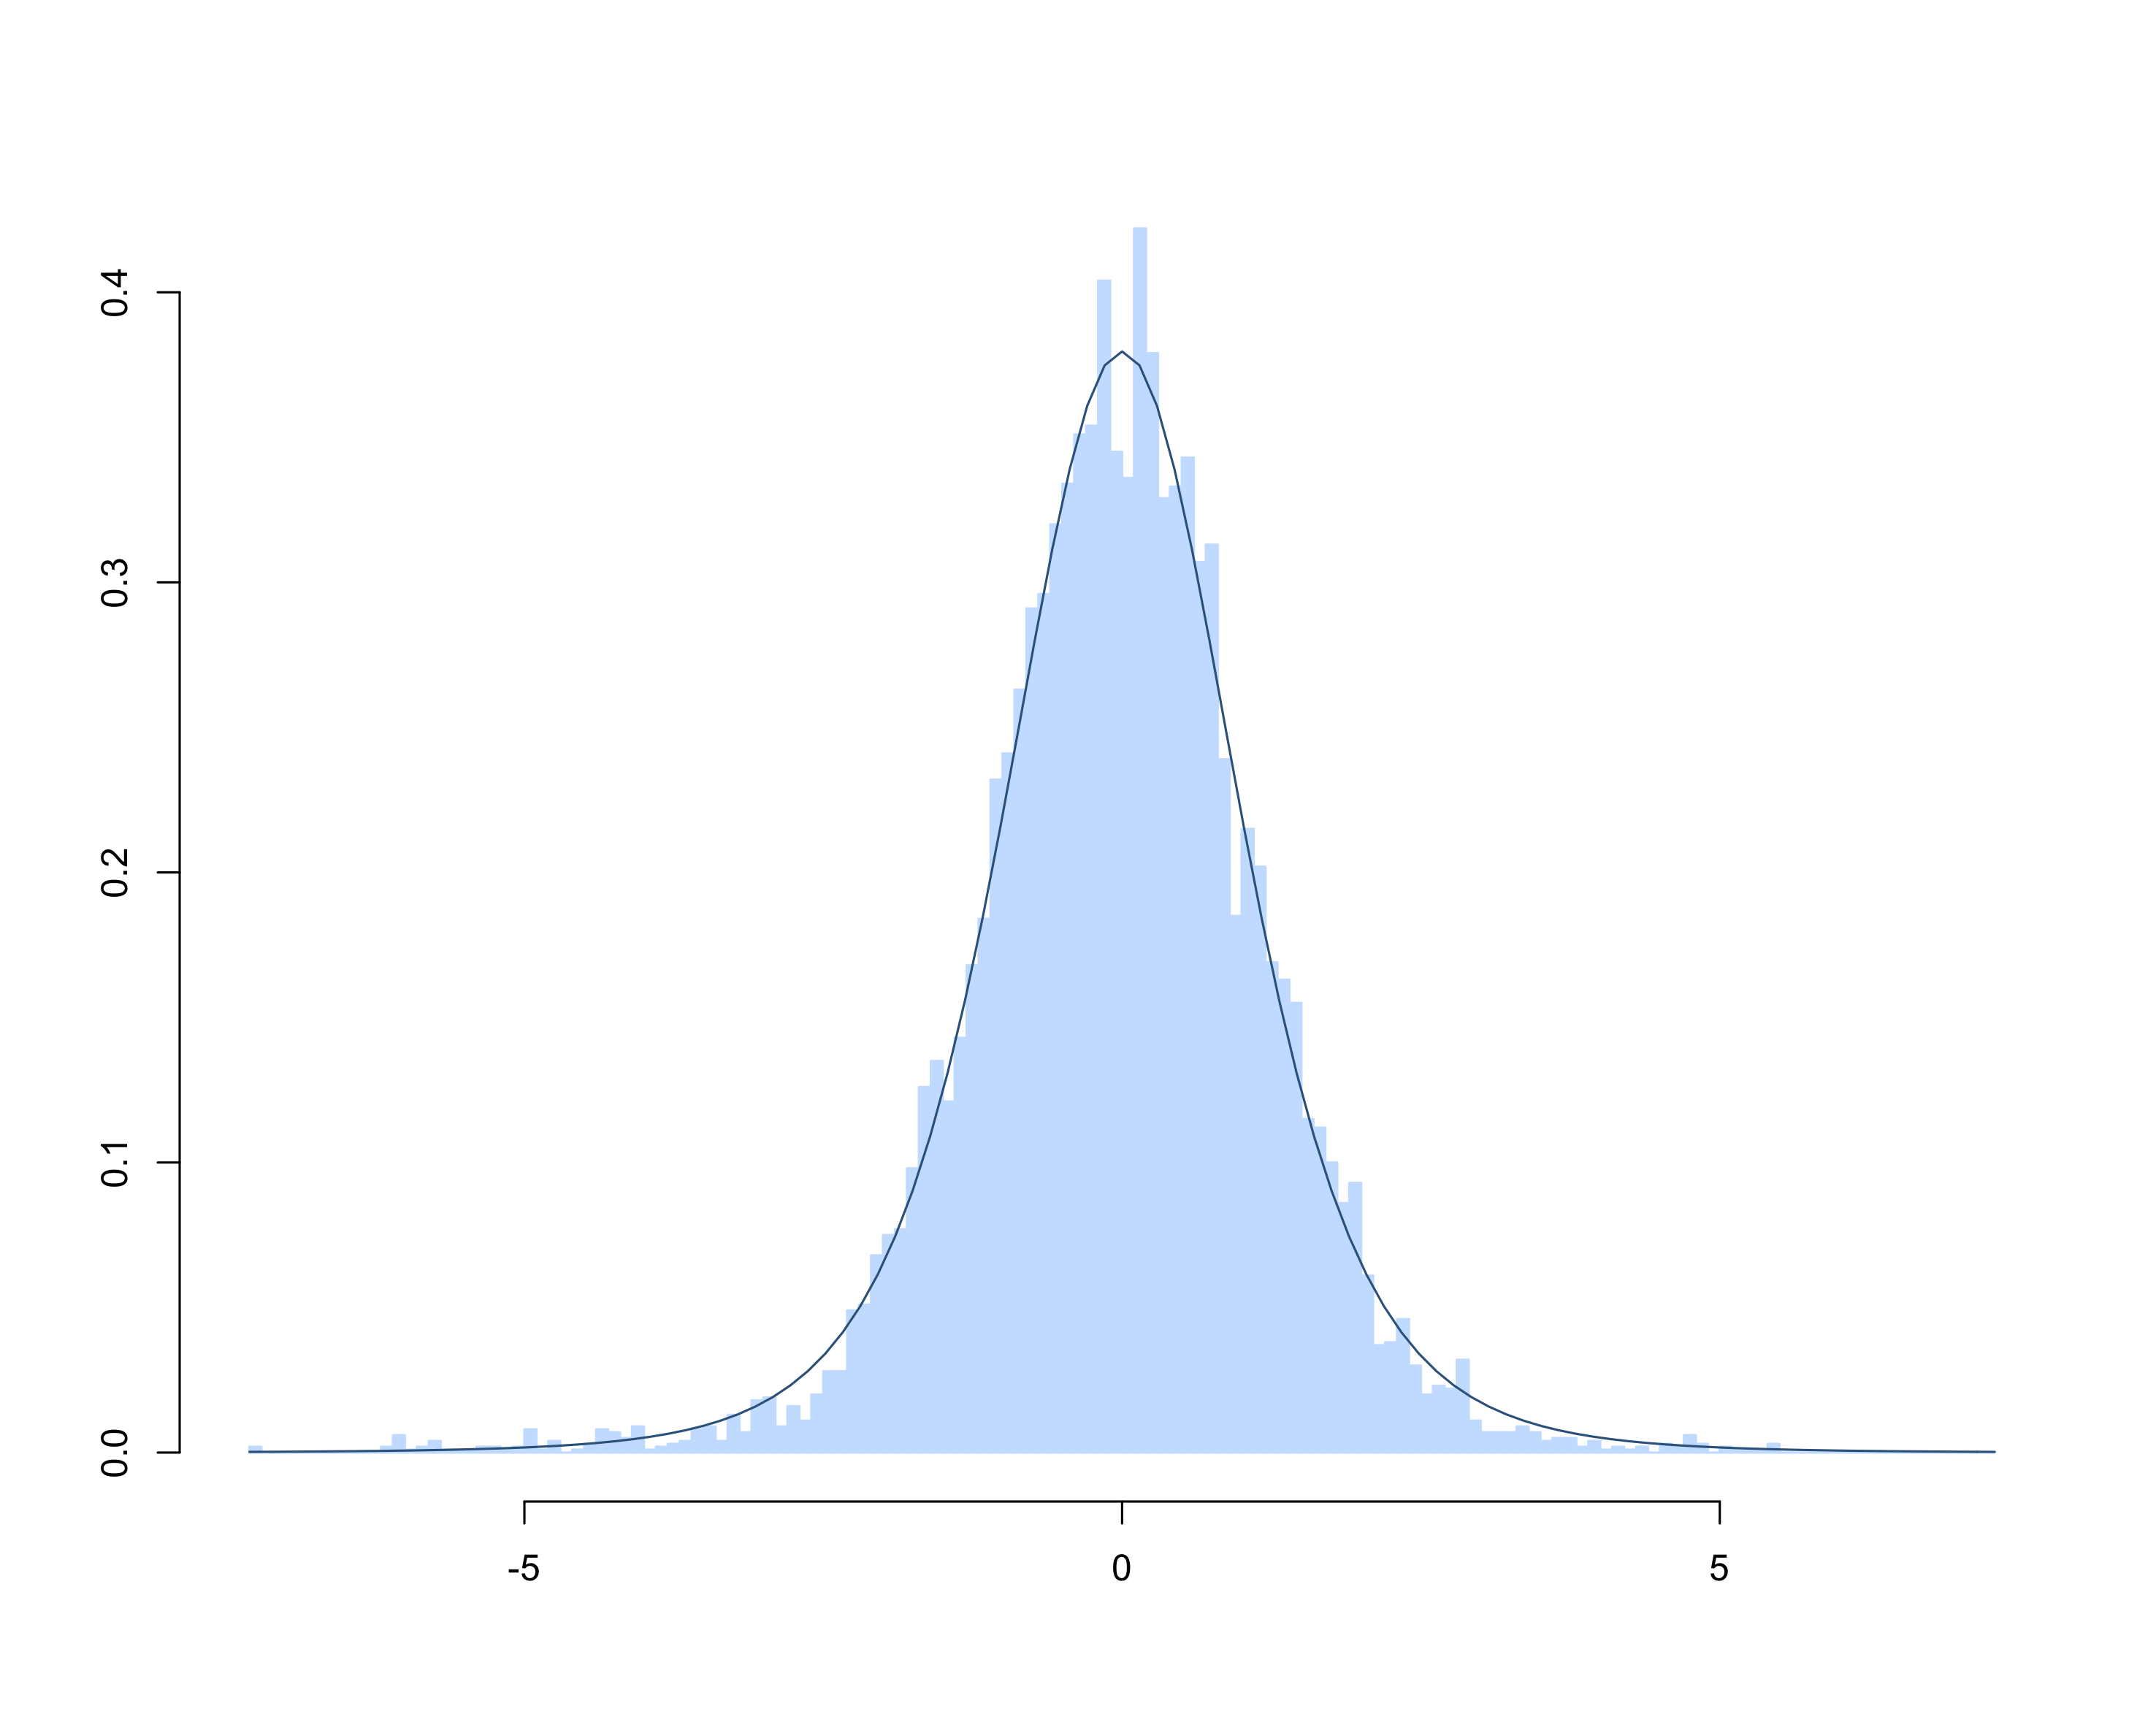
\includegraphics[width=\linewidth]{mh_hist_x2.png} 
        \caption{Histograma de $f \sim t_{(5)}$ con propuestas $q_2$} \label{fig:mh_hist_x2}
    \end{subfigure}
    \hfill
    \begin{subfigure}[t]{0.45\textwidth}
        \centering
        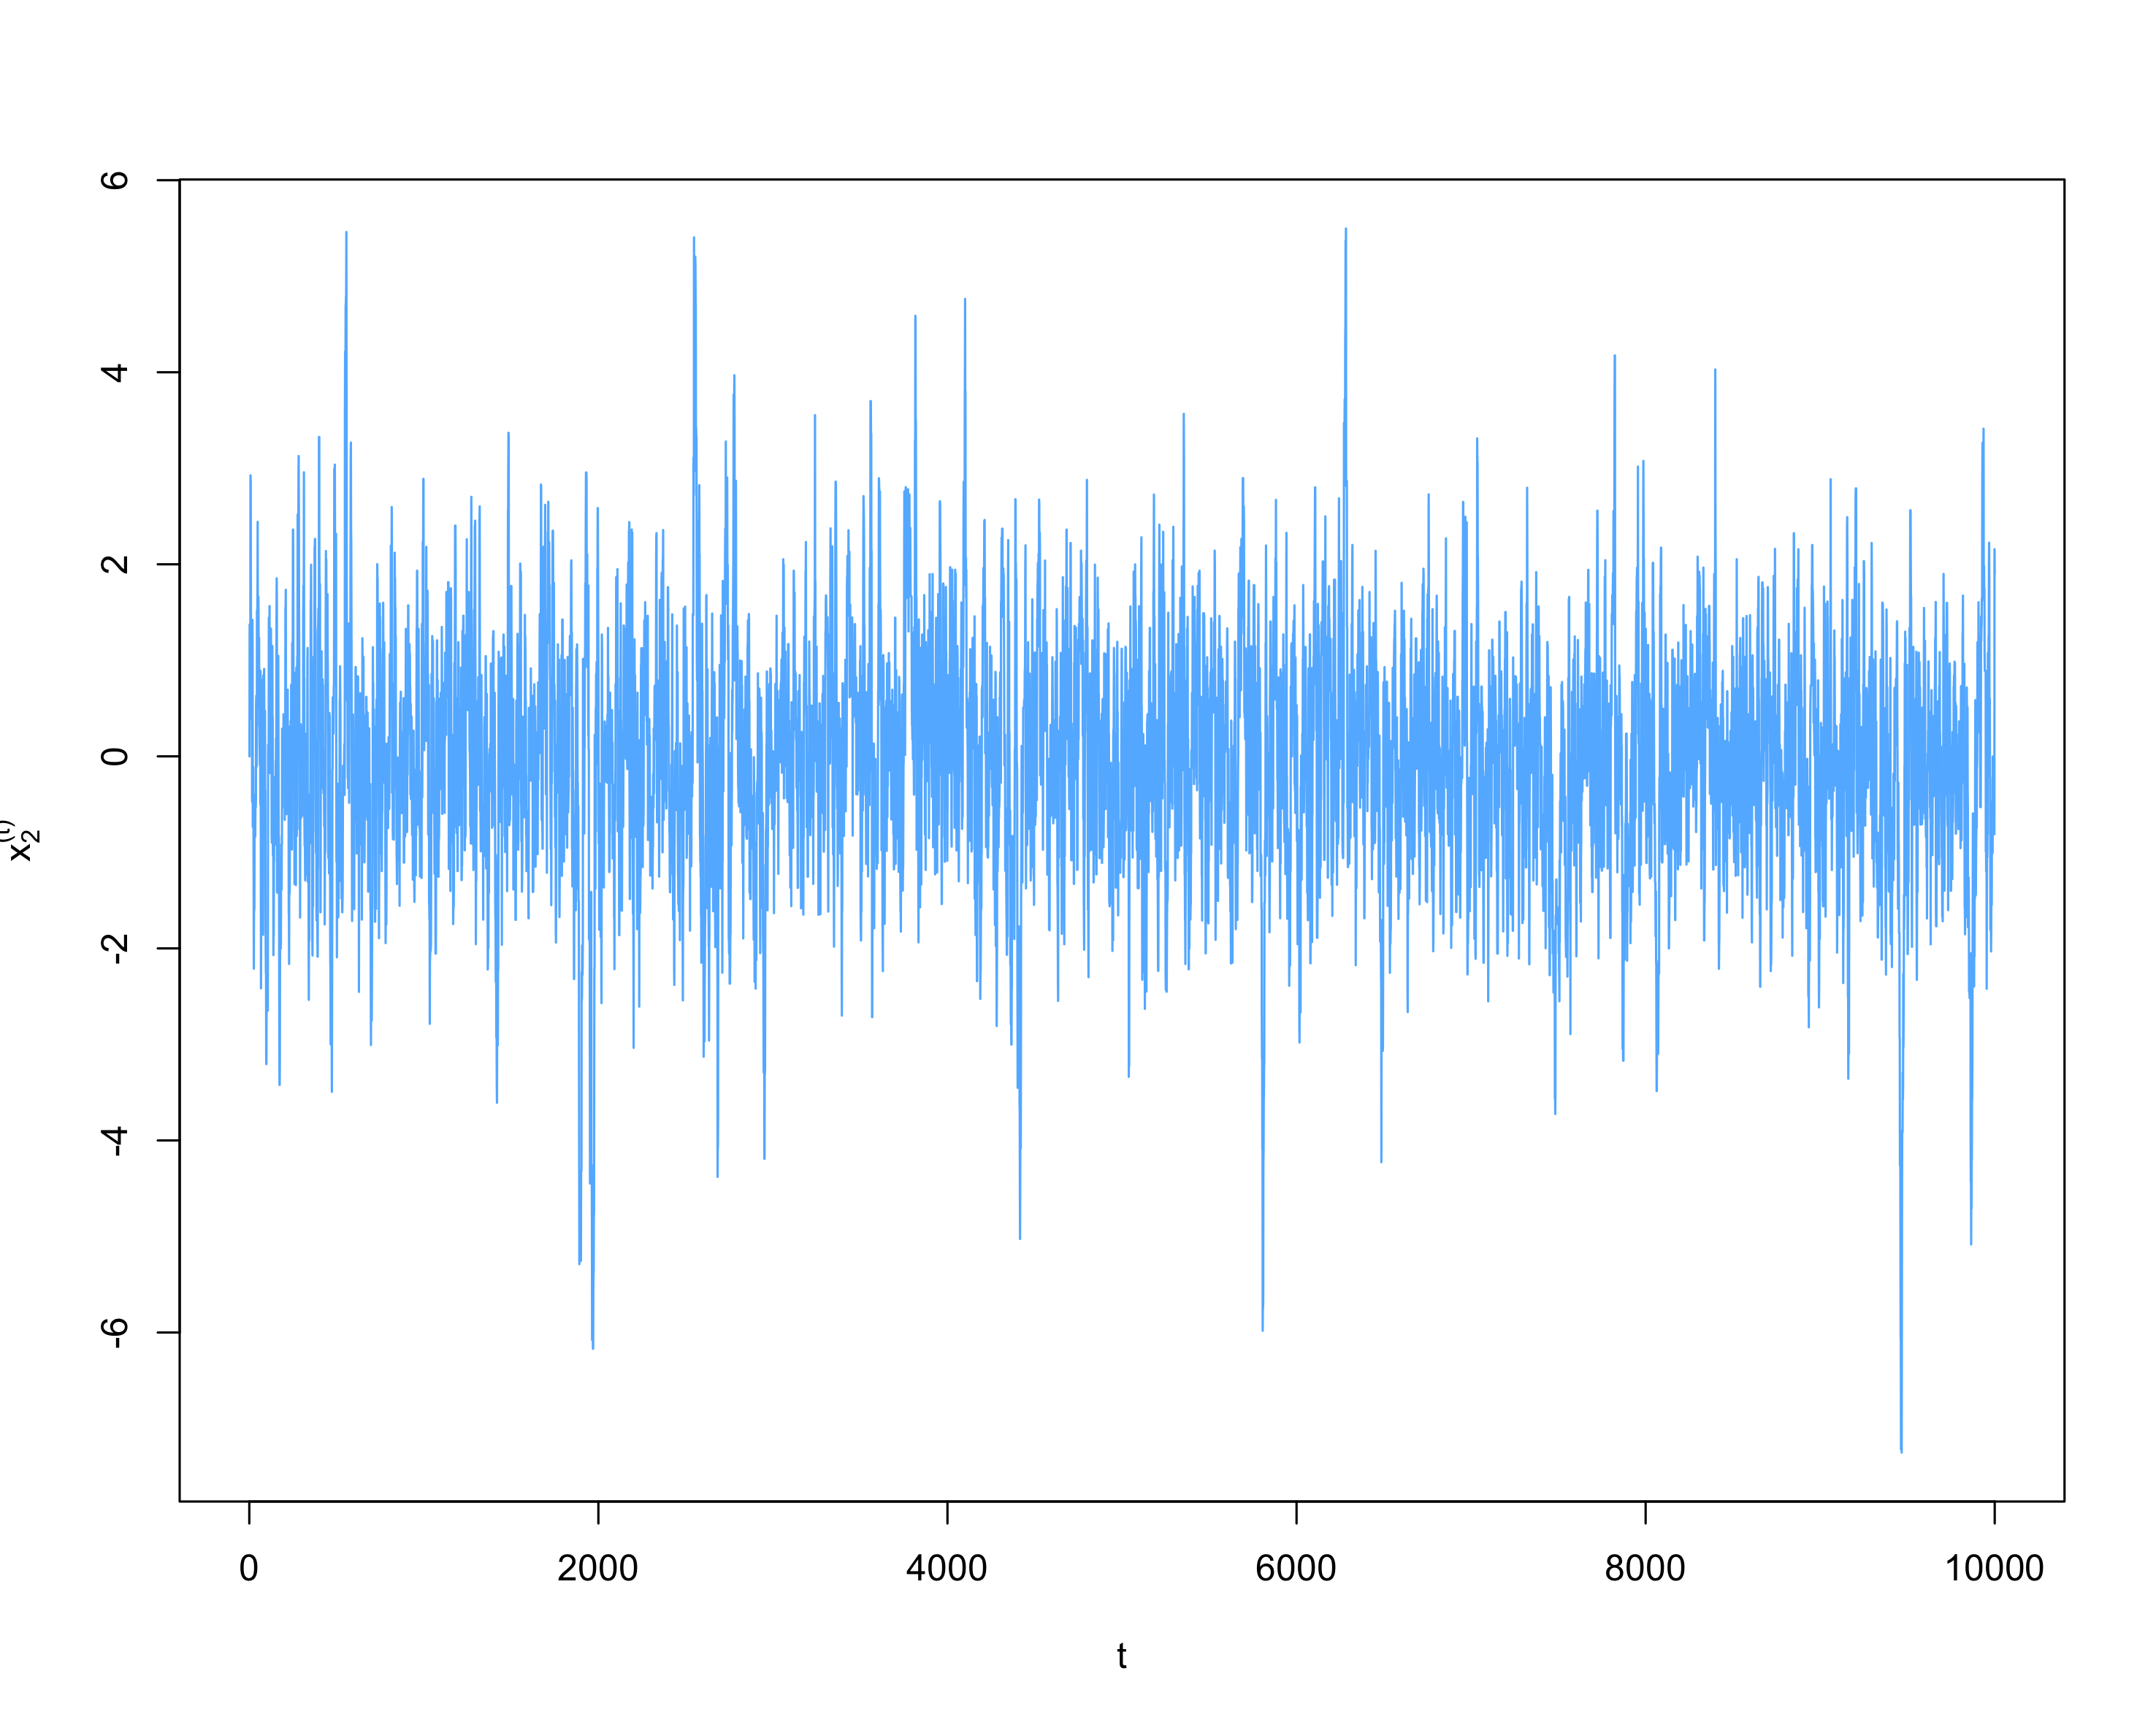
\includegraphics[width=\linewidth]{mh_chain_x2.png} 
        \caption{Proceso $\lbrace X_t^2 \rbrace$} \label{fig:mh_chain_x2}
    \end{subfigure}
    
     \vspace{0.2cm}
    
    \begin{subfigure}[t]{0.45\textwidth}
        \centering
        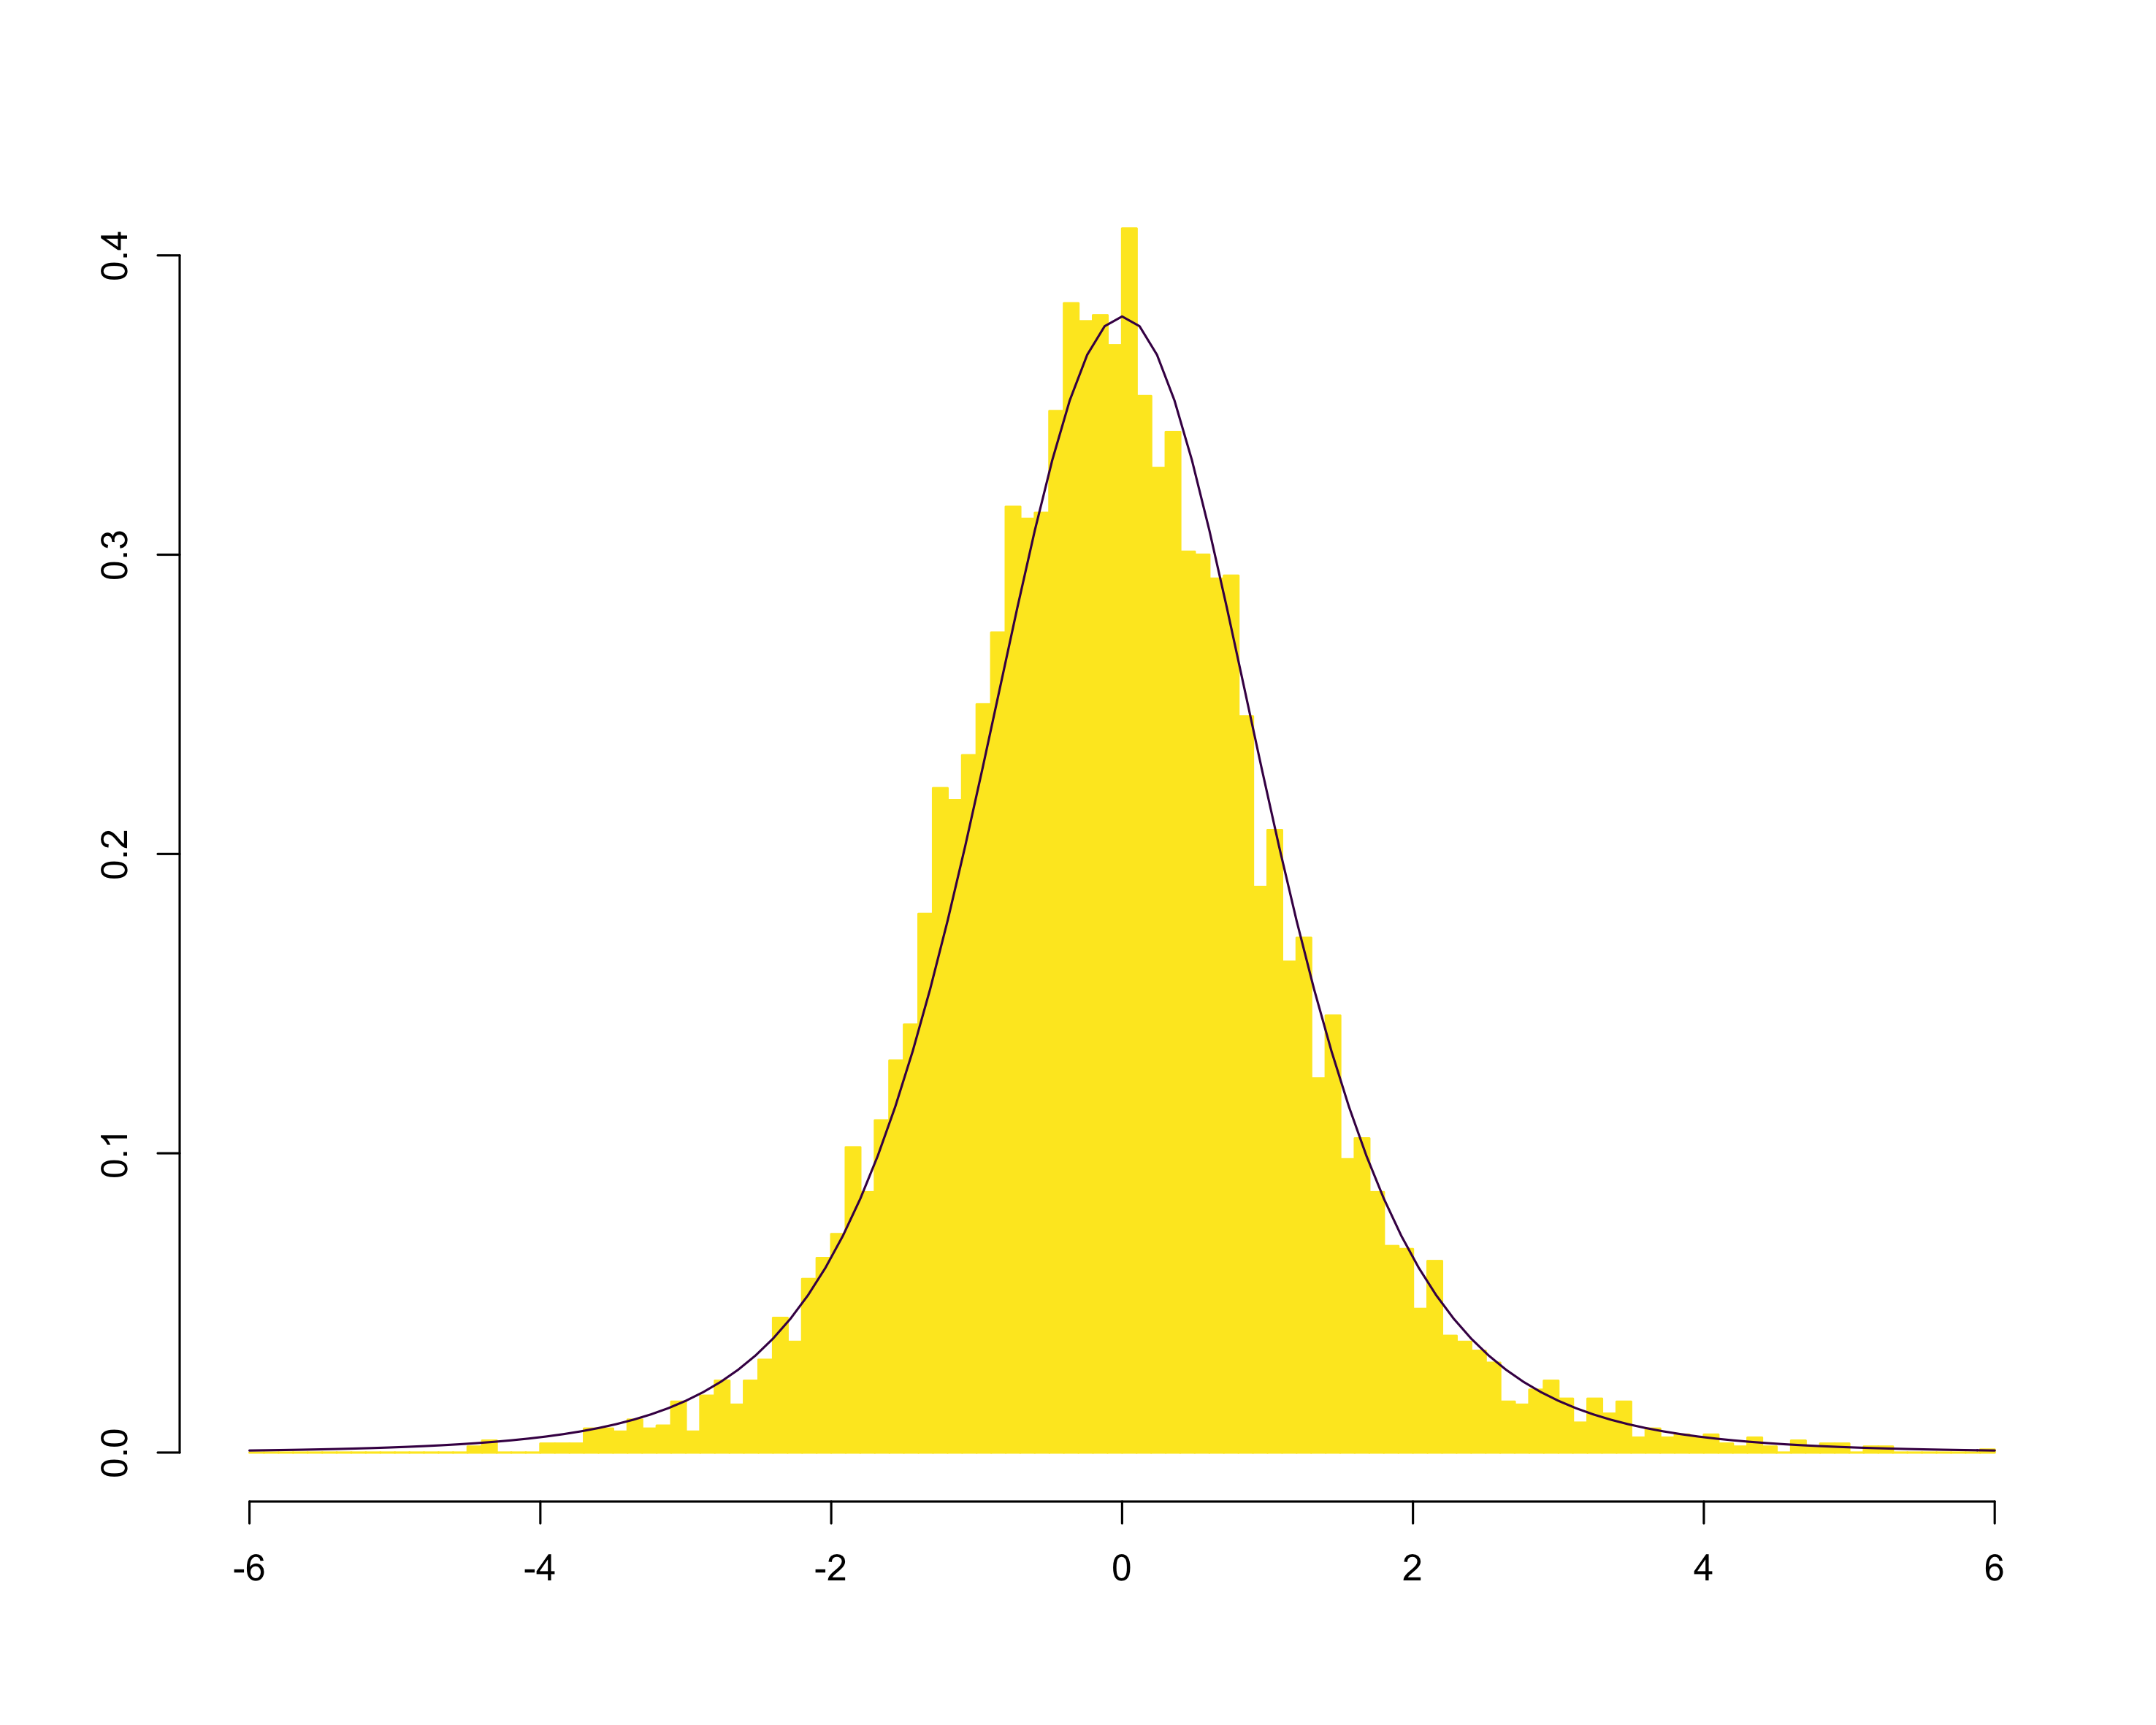
\includegraphics[width=\linewidth]{mh_hist_x3.png} 
        \caption{Histograma de $f \sim t_{(5)}$ con propuestas $q_3$} \label{fig:mh_hist_x3}
    \end{subfigure}
    \hfill
    \begin{subfigure}[t]{0.45\textwidth}
        \centering
        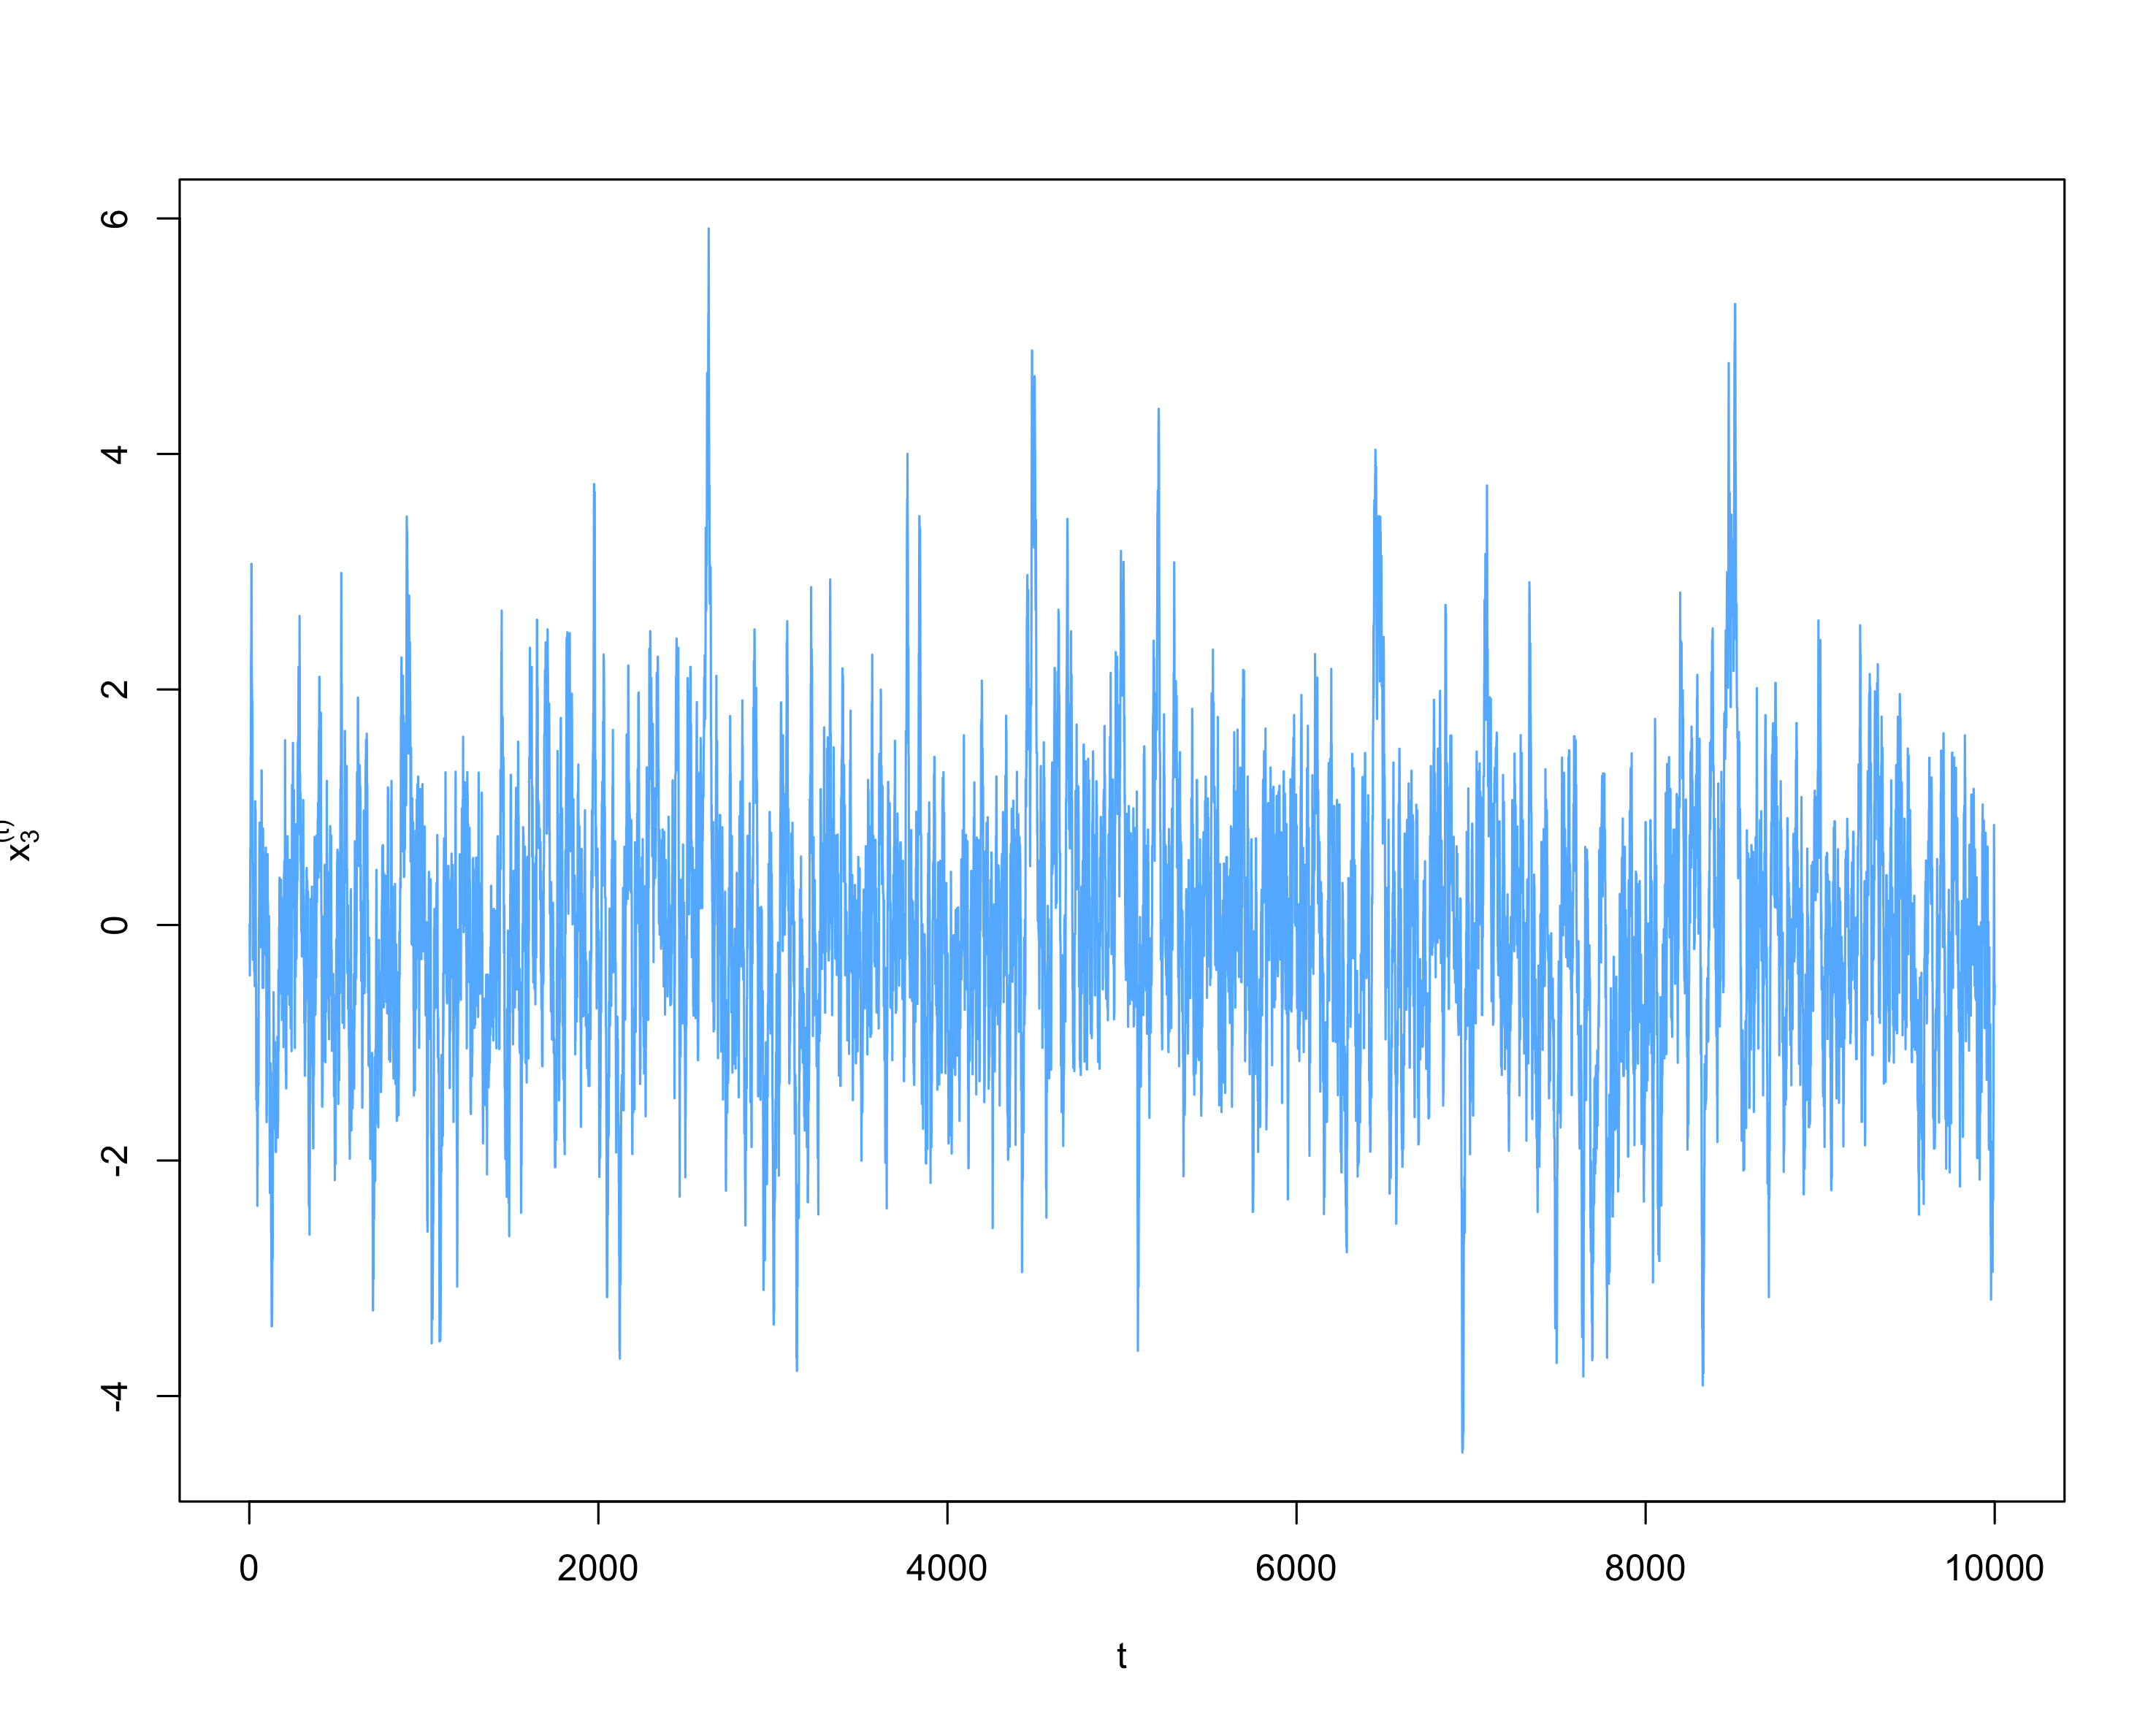
\includegraphics[width=\linewidth]{mh_chain_x3.png} 
        \caption{Proceso $\lbrace X_t^3 \rbrace$} \label{fig:mh_chain_x3}
    \end{subfigure}
    
    \caption{Simulaciones de $X \sim t_{(5)}$ utilizando el algoritmo de Metropolis-Hastings con propuestas $q_1$, $q_2$ y $q_3$}
    \label{fig:mh_t}
\end{figure}

\newpage

Se puede ver en la figura \ref{fig:mh_t} que los tres histogramas parecen ajustarse bien a la distribución $t_{(5)}$, aunque hay algunas diferencias notables. Primero, la cadena con propuestas de la distribución normal estándar es la que tiene un rango más reducido de observaciones, más o menos entre -4 y 4. Esto tiene sentido ya que la distribución normal tiene colas más ligeras que la $t$, por lo que al proceso le cuesta más explorar valores alejados de la media. Por el contrario, las cadenas con propuestas $q_2$ y $q_3$ abarcan intervalos más amplios. Específicamente, las propuestas con la caminata aleatoria normal son las que exploran un mayor rango de la distribución de interés, alrededor del intervalo $(-6, 6)$. A pesar de estas diferencias, no es obvio a simple vista cuál de las cadenas funciona mejor para simular observaciones de la distribución $t_{(5)}$. Para poder elegir la distribución $q$ se necesitan criterios de selección, basados en diagnósticos de las cadenas.

Hay tres cosas que se deben monitorear en muestras de MCMC \citep{kruschke}:
\begin{enumerate}
\item Convergencia de la cadena a la distribución estacionaria.
\item Precisión y estabilidad de las estimaciones (valores esperados, cuantiles, etc.).
\item Eficiencia en las simulaciones.
\end{enumerate}

Diagnosticar la convergencia a la distribución estacionaria suele ser complejo porque en muchas aplicaciones se desconoce la geometría de la distribución de interés. Por esto, es común utilizar diagnósticos visuales de los estados que visita la cadena en cada iteración. La idea es generar varias cadenas con estados iniciales distintos. Se busca que después de cierto número de iteraciones, las distintas cadenas estén explorando la misma región de la distribución de interés, eliminando la dependencia de los valores iniciales. A estas gráficas se les llama de traza o \textit{trace plots.} Es esencial que este diagnóstico visual utilice múltiples cadenas, ya que si solamente se toma una cadena se puede tener la falsa idea de que la cadena explora de manera eficiente el rango de la distribución. Un ejemplo es si la distribución de interés es bimodal y una cadena explora solamente la vecindad de una de las modas. Es una condición necesaria, más no suficiente de convergencia a la distribución estacionaria que al visualizar las cadenas en la misma gráfica, éstas se encimen y exploren la misma región. Otra visualización que se puede utilizar para este diagnóstico son suavizamientos de los histogramas. Cuando las cadenas convergen a la distribución estacionaria, sus histogramas deben ser parecidos. El suavizamiento se hace para facilitar la visualización simultánea de distintas cadenas.

Es una práctica común (\citet{kruschke}, \citet{gelman} y \citet{casella}) que se descarten las primeras iteraciones de los algoritmos para eliminar la dependencia de los valores iniciales. A estas observaciones descartadas se les llama período de calentamiento o \textit{burn-in}. No existe una regla universal que diga cuál es la longitud necesaria de \textit{burn-in}. Ésta se debe elegir examinando las trazas de las cadenas.

Un diagnóstico numérico que se puede utilizar es la varianza dentro y entre cadenas. La idea de este diagnóstico es que, si una cadena no explora el rango completo de la distribución objetivo, entonces la varianza de esa cadena va a subestimar la varianza de la distribución, aproximándose a la verdadera varianza en el límite. Esto se compara con un promedio ponderado de las varianzas dentro y entre cadenas, el cual es un estimador insesgado de la varianza de la distribución objetivo cuando las observaciones vienen de ésta \citep{gelman}.

Respecto a la precisión y estabilidad de las cantidades estimadas, es muy importante recalcar que las observaciones simuladas con los algoritmos de MCMC no son independientes. Esto significa que los algoritmos de MCMC no exploran la distribución objetivo de manera tan eficiente como lo hacen los algoritmos de las secciones \ref{sec:transformada} y \ref{aceptacion}. Específicamente, mientras mayor sea la correlación entre observaciones, menor es la eficiencia en la exploración. Para diagnosticar esto, se utilizan gráficos de autocorrelación. Estas figuras muestran la correlación que hay entre los valores de la cadena y esos mismos valores desplazados $k$ períodos. También existe un diagnóstico numérico para cuantificar el efecto de la correlación en las observaciones. Se le conoce como tamaño de muestra efectivo o \textit{effective sample size} e intuitivamente dice el tamaño de muestra que se necesitaría para obtener la misma información si las observaciones se generaran de manera independiente \citep{kruschke}.

Finalmente, es recomendable que las simulaciones sean lo más eficientes posible. Es decir, que se tenga la mayor cantidad de información en el menor tiempo. Esto se puede lograr explorando distintas opciones al seleccionar algoritmos y distribuciones candidatas, al igual que realizando simulaciones en paralelo y explotando al máximo los recursos computacionales disponibles.

Antes de cerrar este capítulo, es importante comentar que distintos algoritmos de MCMC, además del muestreador de Gibbs y Metropolis-Hastings, se han desarrollado y son cada vez más comunes en la comunidad estadística. Especialmente hay que resaltar los algoritmos de Monte Carlo Hamiltoniano, los cuales utilizan nociones físicas y de sistemas dinámicos para explorar de manera eficiente las distribuciones. Estos métodos son especialmente útiles en grandes dimensiones porque incorporan información de la geometría de la distribución. El uso de Monte Carlo Hamiltoniano ha ido en aumento en gran parte gracias al software Stan \citep{stan}, el cual implementa este algoritmo y cuenta con interfaces para algunos de los lenguajes de programación más populares como R y Python. Se puede consultar más sobre Monte Carlo Hamiltoniano en \citet{neal}, \citet{betancourt} y \citet{gelman}. Para mayor información sobre el software Stan se recomienda consultar \citet{gelman}, \citet{kruschke} y el sitio web del software\footnote{ \url{https://mc-stan.org}} que contiene manuales e información de libre acceso. También es importante mencionar 
que la mayoría (si no es que todos) los diagnósticos mencionados para simulaciones de MCMC están disponibles en el paquete \texttt{coda} de R \citep{coda}.

\newpage

\section{Modelo de supervivencia basado en cópulas}
\label{elmodelo}

El modelo bayesiano semiparamétrico de \citet{nieto} es un modelo de supervivencia multivariado cuyo objetivo es lidiar con la correlación entre tiempos de fallo de manera adecuada, manteniendo esta estructura de dependencia simple y utilizando densidades marginales no paramétricas para que sean lo más flexibles posible. En este capítulo se explica la construcción y la implementación del modelo.

\subsection{Caso univariado}

Para introducir las ideas, se explica primero el caso univariado. Sea $T$ una variable aleatoria con soporte $\Omega_T = [0, \infty)$ y sean $h$ y $H$ la función de riesgo y riesgo acumulado respectivamente. Interesa escribir la función de densidad $f$ como una mezcla de la forma
\begin{equation} \label{mezcla}
f(t) = \int_{\Omega_\omega} f(t|\omega)m(\omega) \ d\omega,
\end{equation}
donde $\Omega_\omega$ es el soporte de $\omega$. El resultado siguiente muestra que se puede escribir $f(t)$ de la forma \eqref{mezcla}.
\begin{proposition}
Sean $f(t|\omega) = \frac{h(t)}{\omega} \ \mathbb{I}\lbrace\omega > H(t)\rbrace$ y $\omega\sim Ga(\omega | 2, 1)$. Entonces se cumple la representación como mezcla dada por \eqref{mezcla}.
\end{proposition}
\begin{proof}
\begin{align*}
\omega \sim Ga(\omega | 2, 1) &\implies m(\omega) = \omega e^{-\omega} \ (\omega\geq 0)\\
&\implies f(t|\omega)m(\omega) = h(t)e^{-\omega} \ \mathbb{I}\lbrace\omega > H(t)\rbrace.
\end{align*}
Así,
\begin{align*}
\int_{\Omega_\omega} f(t|\omega)m(\omega) \ d\omega &= \int_{H(t)}^\infty h(t)e^{-\omega} \ d\omega\\
&= h(t) \exp(-H(t))\\
&= h(t)S(t)\\
&= f(t).
\end{align*}
\end{proof}

El objetivo es utilizar esta representación como mezcla para introducir la estructura de dependencia a través de variables latentes con distribuciones marginales $Ga(2, 1)$ y no directamente a través de la distribución de los tiempos de fallo.

\subsection{Caso bivariado} \label{caso_bivariado}
Sea ahora $T=(T_1, T_2)$ un vector aleatorio con soporte $\Omega_T = [0, \infty) \times [0, \infty)$ y función de densidad conjunta $f(t_1, t_2)$. Generalizando la idea \eqref{mezcla}, se escribe la densidad conjunta como
\begin{equation} \label{mezcla_conjunta}
f(t_1, t_2) =\int_{\Omega_{\omega_2}}\int_{\Omega_{\omega_1}} f(t_1, t_2 | \omega_1, \omega_2)m(\omega_1, \omega_2) \ d\omega_1 d\omega_2.
\end{equation}
Del modelo univariado se sabe que las densidades marginales condicionales se pueden escribir como en \eqref{mezcla} con
\begin{equation} \label{marginal}
f_j(t|\omega_j) = \frac{h_j(t)}{\omega_j} \ \mathbb{I}\lbrace\omega_j > H(t)\rbrace
\end{equation}
y $\omega_j \sim Ga(2, 1)$.

Ahora se asume independencia condicional de los tiempos de fallo dado $\omega = (\omega_1, \omega_2)$, es decir,
\begin{equation} \label{indcon}
f(t_1, t_2 | \omega_1, \omega_2) = f(t_1 | \omega_1)f(t_2 | \omega_2)\\
\end{equation}
y que $\omega = (\omega_1, \omega_2)$ tiene una distribución gamma bivariada con marginales $Ga(2, 1).$ De esta manera, la construcción definida en las ecuaciones (\ref{mezcla_conjunta} - \ref{indcon}) garantiza que $T_1$ y $T_2$ tienen distribuciones marginales con función de riesgo $h_1(t)$ y $h_2(t)$ respectivamente. Además, la dependencia entre ellos es modelada a través de la dependencia entre $\omega_1$ y $\omega_2$. El siguiente resultado muestra que la construcción definida en las ecuaciones (\ref{mezcla_conjunta} - \ref{indcon}) define una cópula de supervivencia.

\begin{proposition}
La función de supervivencia conjunta obtenida a través de las ecuaciones (\ref{mezcla_conjunta} - \ref{indcon}) define una cópula de supervivencia, esto es, $$S(t_1, t_2) = \widehat{C}(S_1(t_1), S_2(t_2)),$$ donde la cópula de supervivencia $\widehat{C}$ es la función dada por
\begin{align} \label{copula_modelo}
\widehat{C}&(u, v) = \nonumber \\
& \int_{-\log (u)}^\infty \int_{-\log (v)}^\infty \left(1 + \frac{\log(u)}{\omega_1}\right)\left(1 + \frac{\log(v)}{\omega_2}\right) m(\omega_1, \omega_2) \ d\omega_1 d \omega_2.
\end{align}
\end{proposition}
La demostración de esta proposición por medio de la construcción de la cópula se puede consultar en el apéndice \ref{construccion_copula}.

La utilidad de este resultado recae en que se pueden estudiar las medidas de concordancia introducidas en la sección \ref{sec_copulas} sin especificar las distribuciones marginales. Como las integrales que definen $\uptau$ y $\rho$ no se pueden resolver analíticamente, se utilizan las técnicas de integración Monte Carlo introducidas en la sección \ref{sec_cadenas} para aproximarlas. Las expresiones para $\uptau$ y $\rho$ de la sección \ref{sec_copulas} se enunciaron para la correspondiente cópula de distribución dada por la expresión
\begin{align}\label{copula_distribucion}
C(u, v) &= u \ + \ v \ - \ 1 \ +\nonumber\\ 
& \ \ \ \int_{-\log (1-u)}^\infty \int_{-\log (1-v)}^\infty f(u, v, \omega_1, \omega_2) \ d\omega_2 d\omega_1,
\end{align}
donde $f(u, v, \omega_1, \omega_2) = \left( \frac{\log (u)}{\omega_1}+1 \right) \left( \frac{\log (v)}{\omega_2}+1\right) m(\omega_1, \omega_2)$.

La cópula \eqref{copula_distribucion} tiene densidad dada por
\begin{align}
c(u, v) &= \frac{\partial^2C}{\partial v \partial u}\nonumber\\
&= \int_{-\log (1-u)}^\infty \int_{-\log (1-v)}^\infty \frac{m(\omega_1, \omega_2)}{(1-u)(1-v)\omega_1\omega_2} \ d\omega_2 d\omega_1 \nonumber\\
&= E_{m} \left[\frac{\mathbb{I}\lbrace u < 1-e^{-\omega_1}\rbrace \mathbb{I}\lbrace v < 1-e^{-\omega_2} \rbrace}{(1-u)(1-v)\omega_1\omega_2}\right],
\label{eq:densidad_copula}
\end{align}
donde $E_m$ es el valor esperado con respecto a la distribución $m(\omega_1, \omega_2)$. El desarrollo de esta expresión se puede encontrar en el apéndice \ref{sec_densidad_copula_modelo}.

Las integrales en las expresiones de la tau de Kendall (proposición \ref{prop:kendall}) y la rho de Spearman (ecuación \eqref{volumen})  para una cópula $C$ se pueden reescribir como valores esperados y utilizar integración Monte Carlo para aproximarlas:
\begin{equation} \label{tau_esperado}
\uptau_{C} = 4 \ E_{(U, V)}\left[C(u, v) c(u, v)\right] -1,
\end{equation}
\begin{equation} \label{rho_esperado}
\rho_{C} = 12 \ E_{(U, V)}\left[C(u, v)\right] -3,
\end{equation}
donde $E_{(U, V)}$ es el valor esperado respecto a una densidad uniforme en \newline $(0, 1)\times (0, 1)$ con componentes independientes. Se escribe también la integral de la cópula \eqref{copula_distribucion} como un valor esperado:
\begin{align}
C(u, v) = &u \ + \ v \ - \ 1 \ +\nonumber\\
E_{m} & \left[\mathbb{I}\lbrace u < 1-e^{-\omega_1}\rbrace\left(1 + \frac{\log (1-u)}{\omega_1}\right) \right.\nonumber\\
& \left. \mathbb{I}\lbrace v < 1-e^{-\omega_2}\rbrace\left(1 + \frac{\log (1-v)}{\omega_2}\right)\right], \label{eq:copula_mc}
\end{align}
lo cual nos permitirá aproximarla a su vez con integración Monte Carlo. Esto significa que para obtener las aproximaciones de $\uptau_C$ y $\rho_C$ se necesitan dos integraciones Monte Carlo, primero para aproximar la función cópula \eqref{eq:copula_mc} y después para las aproximaciones de las ecuaciones \eqref{tau_esperado} y \eqref{rho_esperado}. Además la aproximación de $\uptau_C$ requiere una integración Monte Carlo adicional para aproximar la densidad de la cópula \eqref{eq:densidad_copula}.

Lo único que falta para realizar las aproximaciones es especificar la distribución $m(\omega_1, \omega_2)$ para simular observaciones y aproximar las integrales. \citet{nieto} introducen esta distribución de la siguiente forma. Sea
\begin{align*}
\omega_j | y &\sim Ga(a + y, b + \gamma)\\
y &\sim Pg(a, b, \gamma),
\end{align*}
donde $Pg$ se refiere a la distribución Poisson-gamma introducida en la sección \ref{sec:transformada}. Con esta definición se tiene que el vector aleatorio $(\omega_1, \omega_2)$ tiene una distribución gamma bivariada con parámetros $a, b, \gamma > 0$, denotada $BGa(a, b, \gamma)$. Marginalmente, $\omega_j \sim Ga(a, b)$ y se tiene además que $$corr(\omega_1, \omega_2) = \frac{\gamma}{b + \gamma}.$$ Esta construcción solamente permite una correlación positiva entre $\omega_1$ y $\omega_2$. En caso de requerir correlación negativa se necesitaría utilizar una distribución gamma bivariada distinta \citep{nieto}.

Ahora, como en \eqref{marginal} se requiere que las $\omega_j$ tengan una distribución $Ga(2, 1)$, se tiene que 
\begin{align} \label{eq_omegas}
\omega_j | y &\sim Ga(2 + y, 1 + \gamma) \nonumber\\
y &\sim Pg(2, 1, \gamma) \text{ y} \\
corr(\omega_1, \omega_2) &= \frac{\gamma}{1 + \gamma}. \nonumber
\end{align}
Así, el único parámetro necesario para definir la distribución es $\gamma$ y se tiene que $(\omega_1, \omega_2) \sim BGa(2, 1, \gamma), \ \gamma >0$. Con esta construcción de $m(\omega_1, \omega_2)$, se pueden ya realizar las aproximaciones de $\uptau_C$ y $\rho_C$. Se incluyen gráficas y el código para aproximar ambas cantidades como función del parámetro $\gamma$. Primero se definen dos funciones para aproximar el valor de $C(u, v)$ y $c(u, v)$ las cuales se presentan en el cuadro \ref{cod:fun_copula} y una función para obtener muestras de $m(\omega_1, \omega_2)$ incluida en el cuadro \ref{cod:fun_omega}. Una vez definidas estas funciones, se definen las funciones para aproximar $\uptau_C$ (cuadro \ref{cod:kendall_tau}) y $\rho_C$ (cuadro \ref{cod:spearman_rho}). Para ambas aproximaciones se utiliza la misma muestra de $(U, V)$.

\begin{table}[!htb]
\begin{lstlisting}
copula <- function(u, v, omega1, omega2) {
  c <- (1 + log(1 - u) / omega1) * (1 + log(1 - v) / omega2)
  c <- mean(c * (u < 1 - exp(-omega1)) * (v < 1 - exp(-omega2)))
  res <- (u + v - 1 + c) * (u > 0) * (v > 0)
  return(res)
}

densidad_copula <- function(u, v, omega1, omega2) {
  c <- 1 / (1 - u) * 1 / (1 - v) * 1 / (omega1 * omega2)
  c <- mean(c * (u < 1 - exp(-omega1)) * (v < 1 - exp(-omega2)))
  return(c)
}
\end{lstlisting}
\caption{Funciones para aproximar el valor de $C(u, v)$ y $c(u, v)$ en R.}
\label{cod:fun_copula}
\end{table}

\begin{table}[!htb]
\begin{lstlisting}
sim_omega <- function(n.sim, a = 2, b = 1, gamma = 5) {
  lam <- rgamma(n = n.sim, shape = a, rate = b)
  y <- rpois(n = n.sim, lambda = lam * gamma)
  omega1 <- rgamma(n = n.sim, shape = a + y, rate = b + gamma)
  omega2 <- rgamma(n = n.sim, shape = a + y, rate = b + gamma)
  return(list("omega1" = omega1, "omega2" = omega2))
}
\end{lstlisting}
\caption{Función para obtener muestras de $m(\omega_1, \omega_2)$ en R.}
\label{cod:fun_omega}
\end{table}

\begin{table}[!htb]
\begin{lstlisting}
n.sim <- 1e4
set.seed(42)

vec.u <- runif(n.sim)
vec.v <- runif(n.sim)

kendall_tau <- function(gamma) {
  set.seed(42)
  omega <- sim_omega(1e4, gamma = gamma)
  c <- vector(mode = "double", length = length(vec.u))
  dc <- vector(mode = "double", length = length(vec.u))
  for (i in 1:length(vec.u)) {
    u <- vec.u[i]
    v <- vec.v[i]
    c[i] <- copula(u, v, omega$omega1, omega$omega2)
    dc[i] <- densidad_copula(u, v, omega$omega1, omega$omega2)
  }
  return(4 * mean(c * dc) - 1)
}

x <- seq(from = 0, to = 100, by = 1)
y <- vector(mode = "double", length = length(x))

for (i in 1:length(x)) {
  y[i] <- kendall_tau(x[i])
}
\end{lstlisting}
\caption{Función para aproximar $\uptau_C$ en R.}
\label{cod:kendall_tau}
\end{table}

\begin{table}[!htb]
\begin{lstlisting}
spearman_rho <- function(gamma) {
  set.seed(42)
  omega <- sim_omega(1e4, gamma = gamma)
  c <- vector(mode = "double", length = length(vec.u))
  for (i in 1:length(vec.u)) {
    u <- vec.u[i]
    v <- vec.v[i]
    c[i] <- copula(u, v, omega$omega1, omega$omega2)
  }
  return(12 * mean(c) - 3)
}

rho <- vector(mode = "double", length = length(x))

for (i in 1:length(x)) {
  rho[i] <- spearman_rho(x[i])
}
\end{lstlisting}
\caption{Función para aproximar $\rho_C$ en R.}
\label{cod:spearman_rho}
\end{table}

En la figura \ref{fig:kendall_tau} se puede ver que $\uptau_C$ es una función creciente de $\gamma$. Además, parece tener un comportamiento asintótico alrededor de $\uptau_C = 0.3$. Del mismo modo, en la figura \ref{fig:spearman_rho} se ve que $\rho_C$ es una función creciente de $\gamma$ con un comportamiento asintótico alrededor de $\rho_C = 0.4$. 

\begin{figure}[!htb]
\centering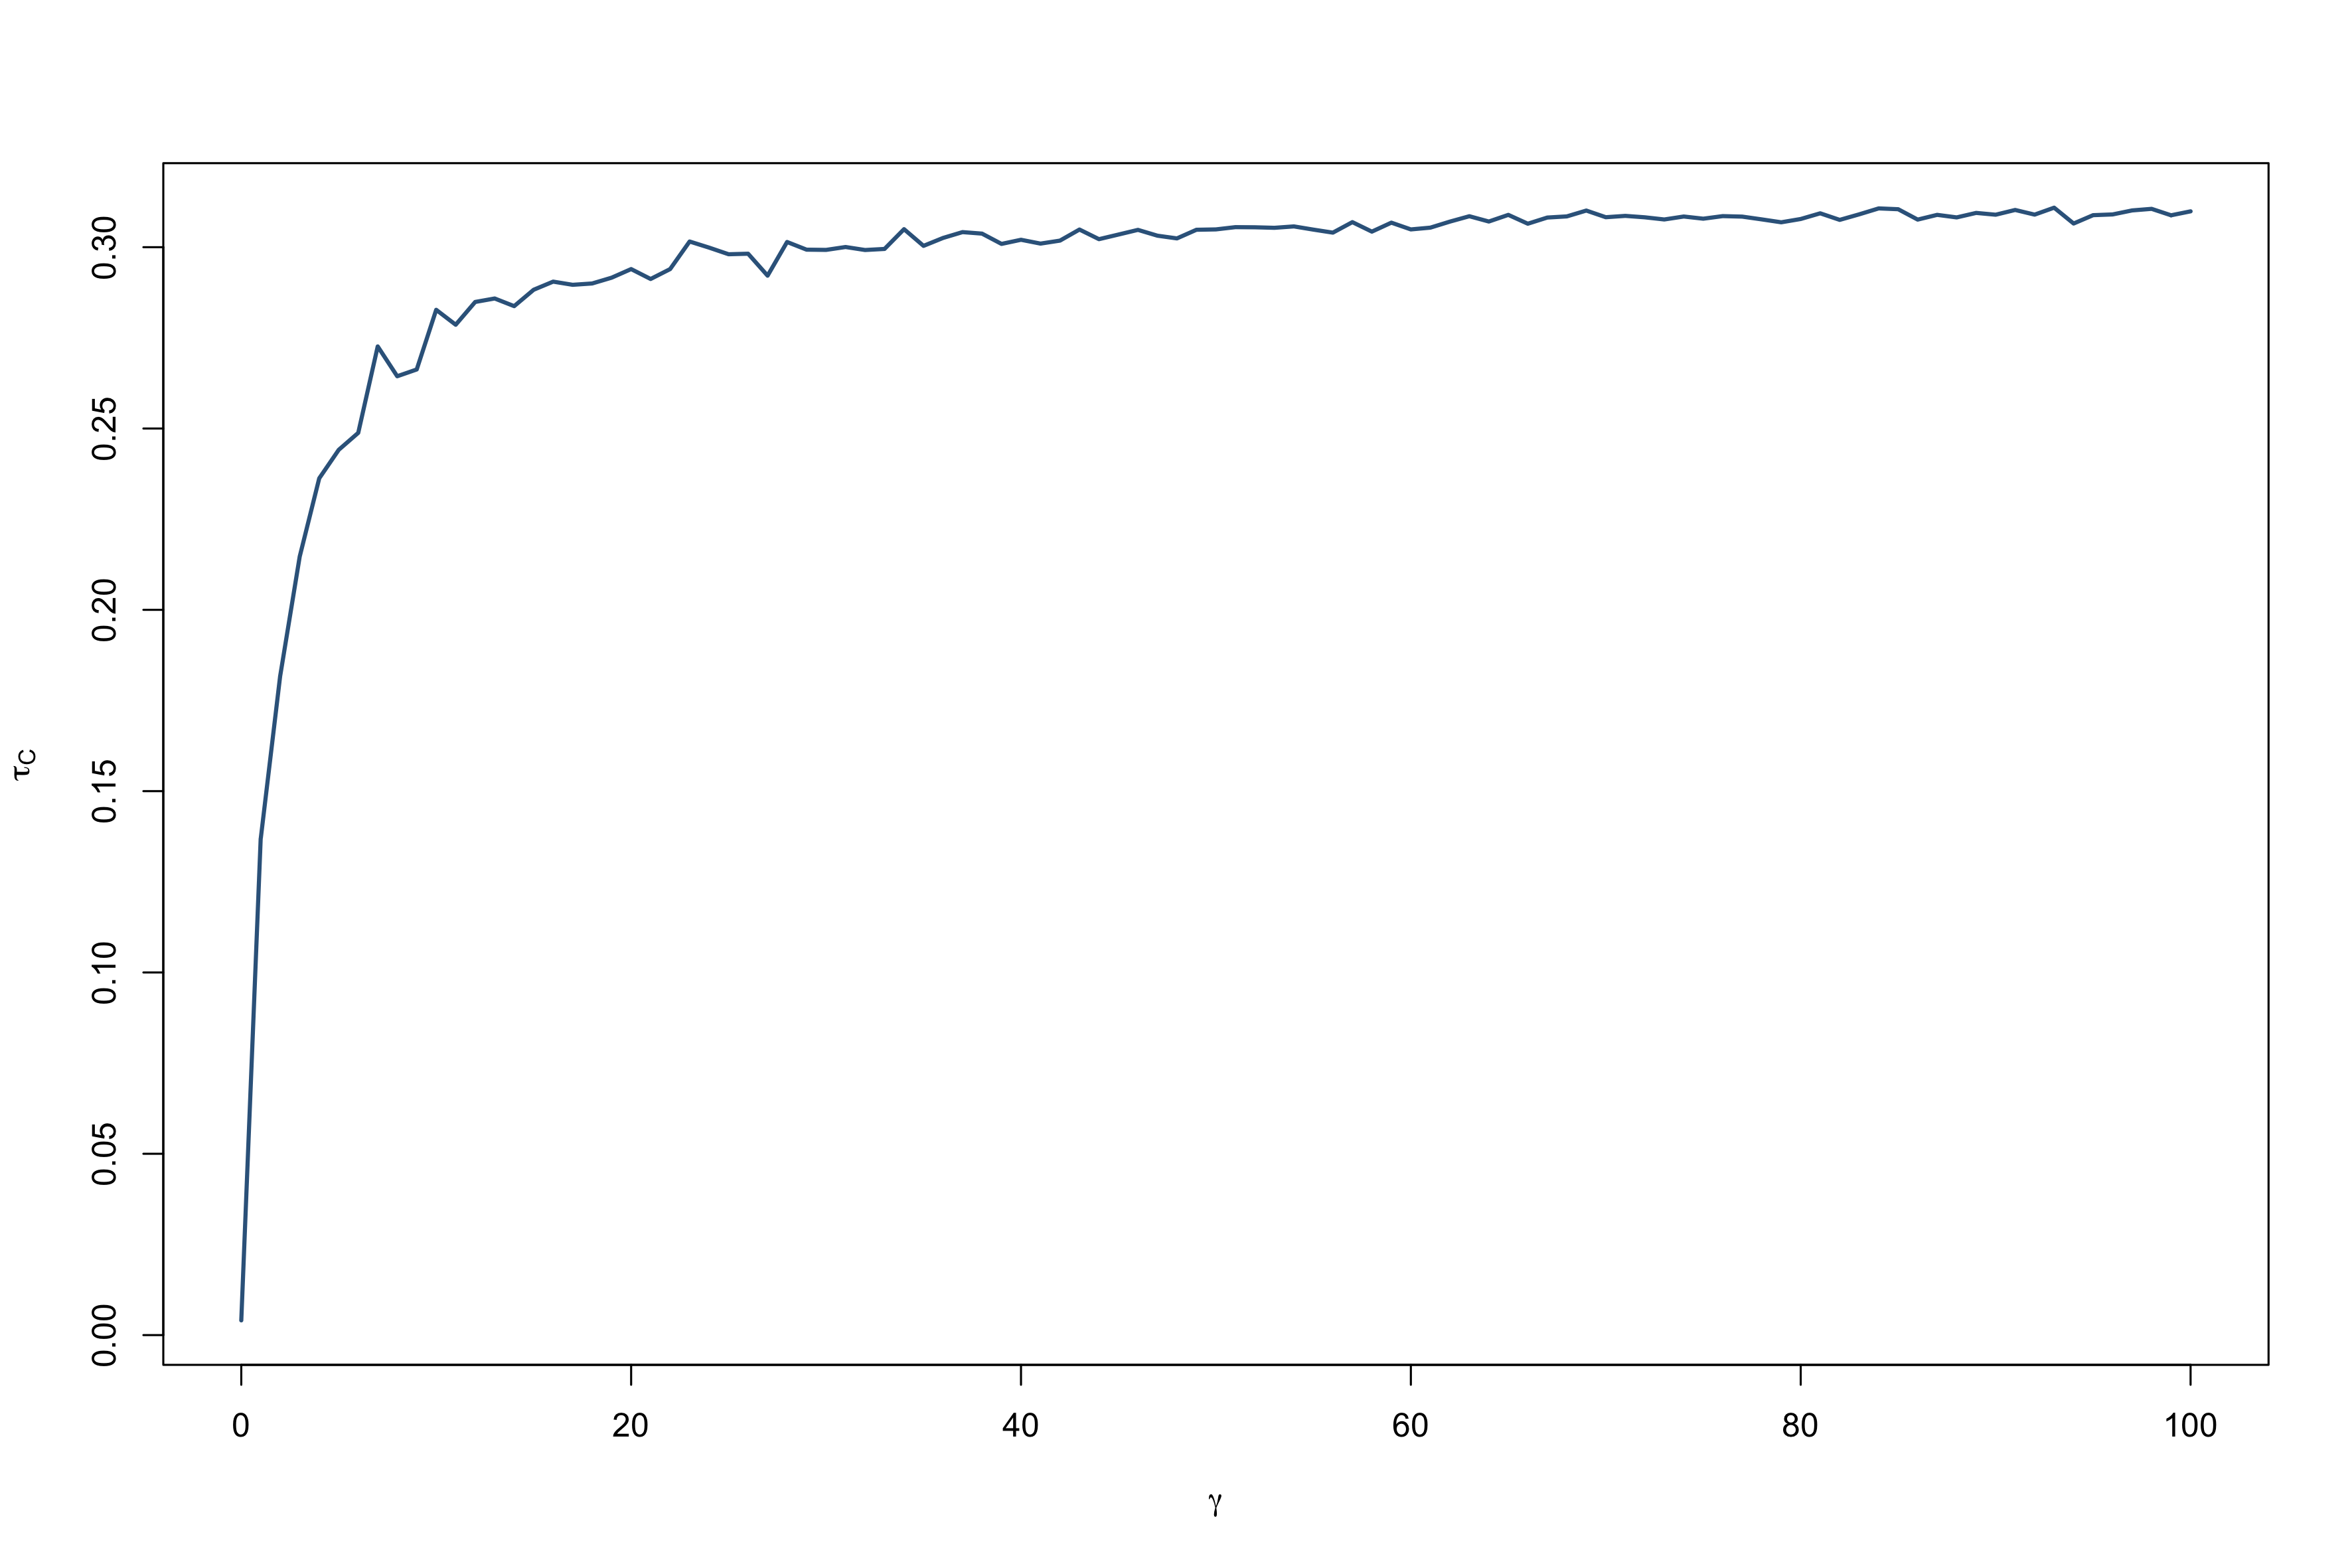
\includegraphics[width=10cm]{kendall_tau.png}
\caption{Gráfica de la tau de Kendall en función de gamma: $\uptau_C (\gamma)$.}
\label{fig:kendall_tau}
\end{figure}

\begin{figure}[!htb]
\centering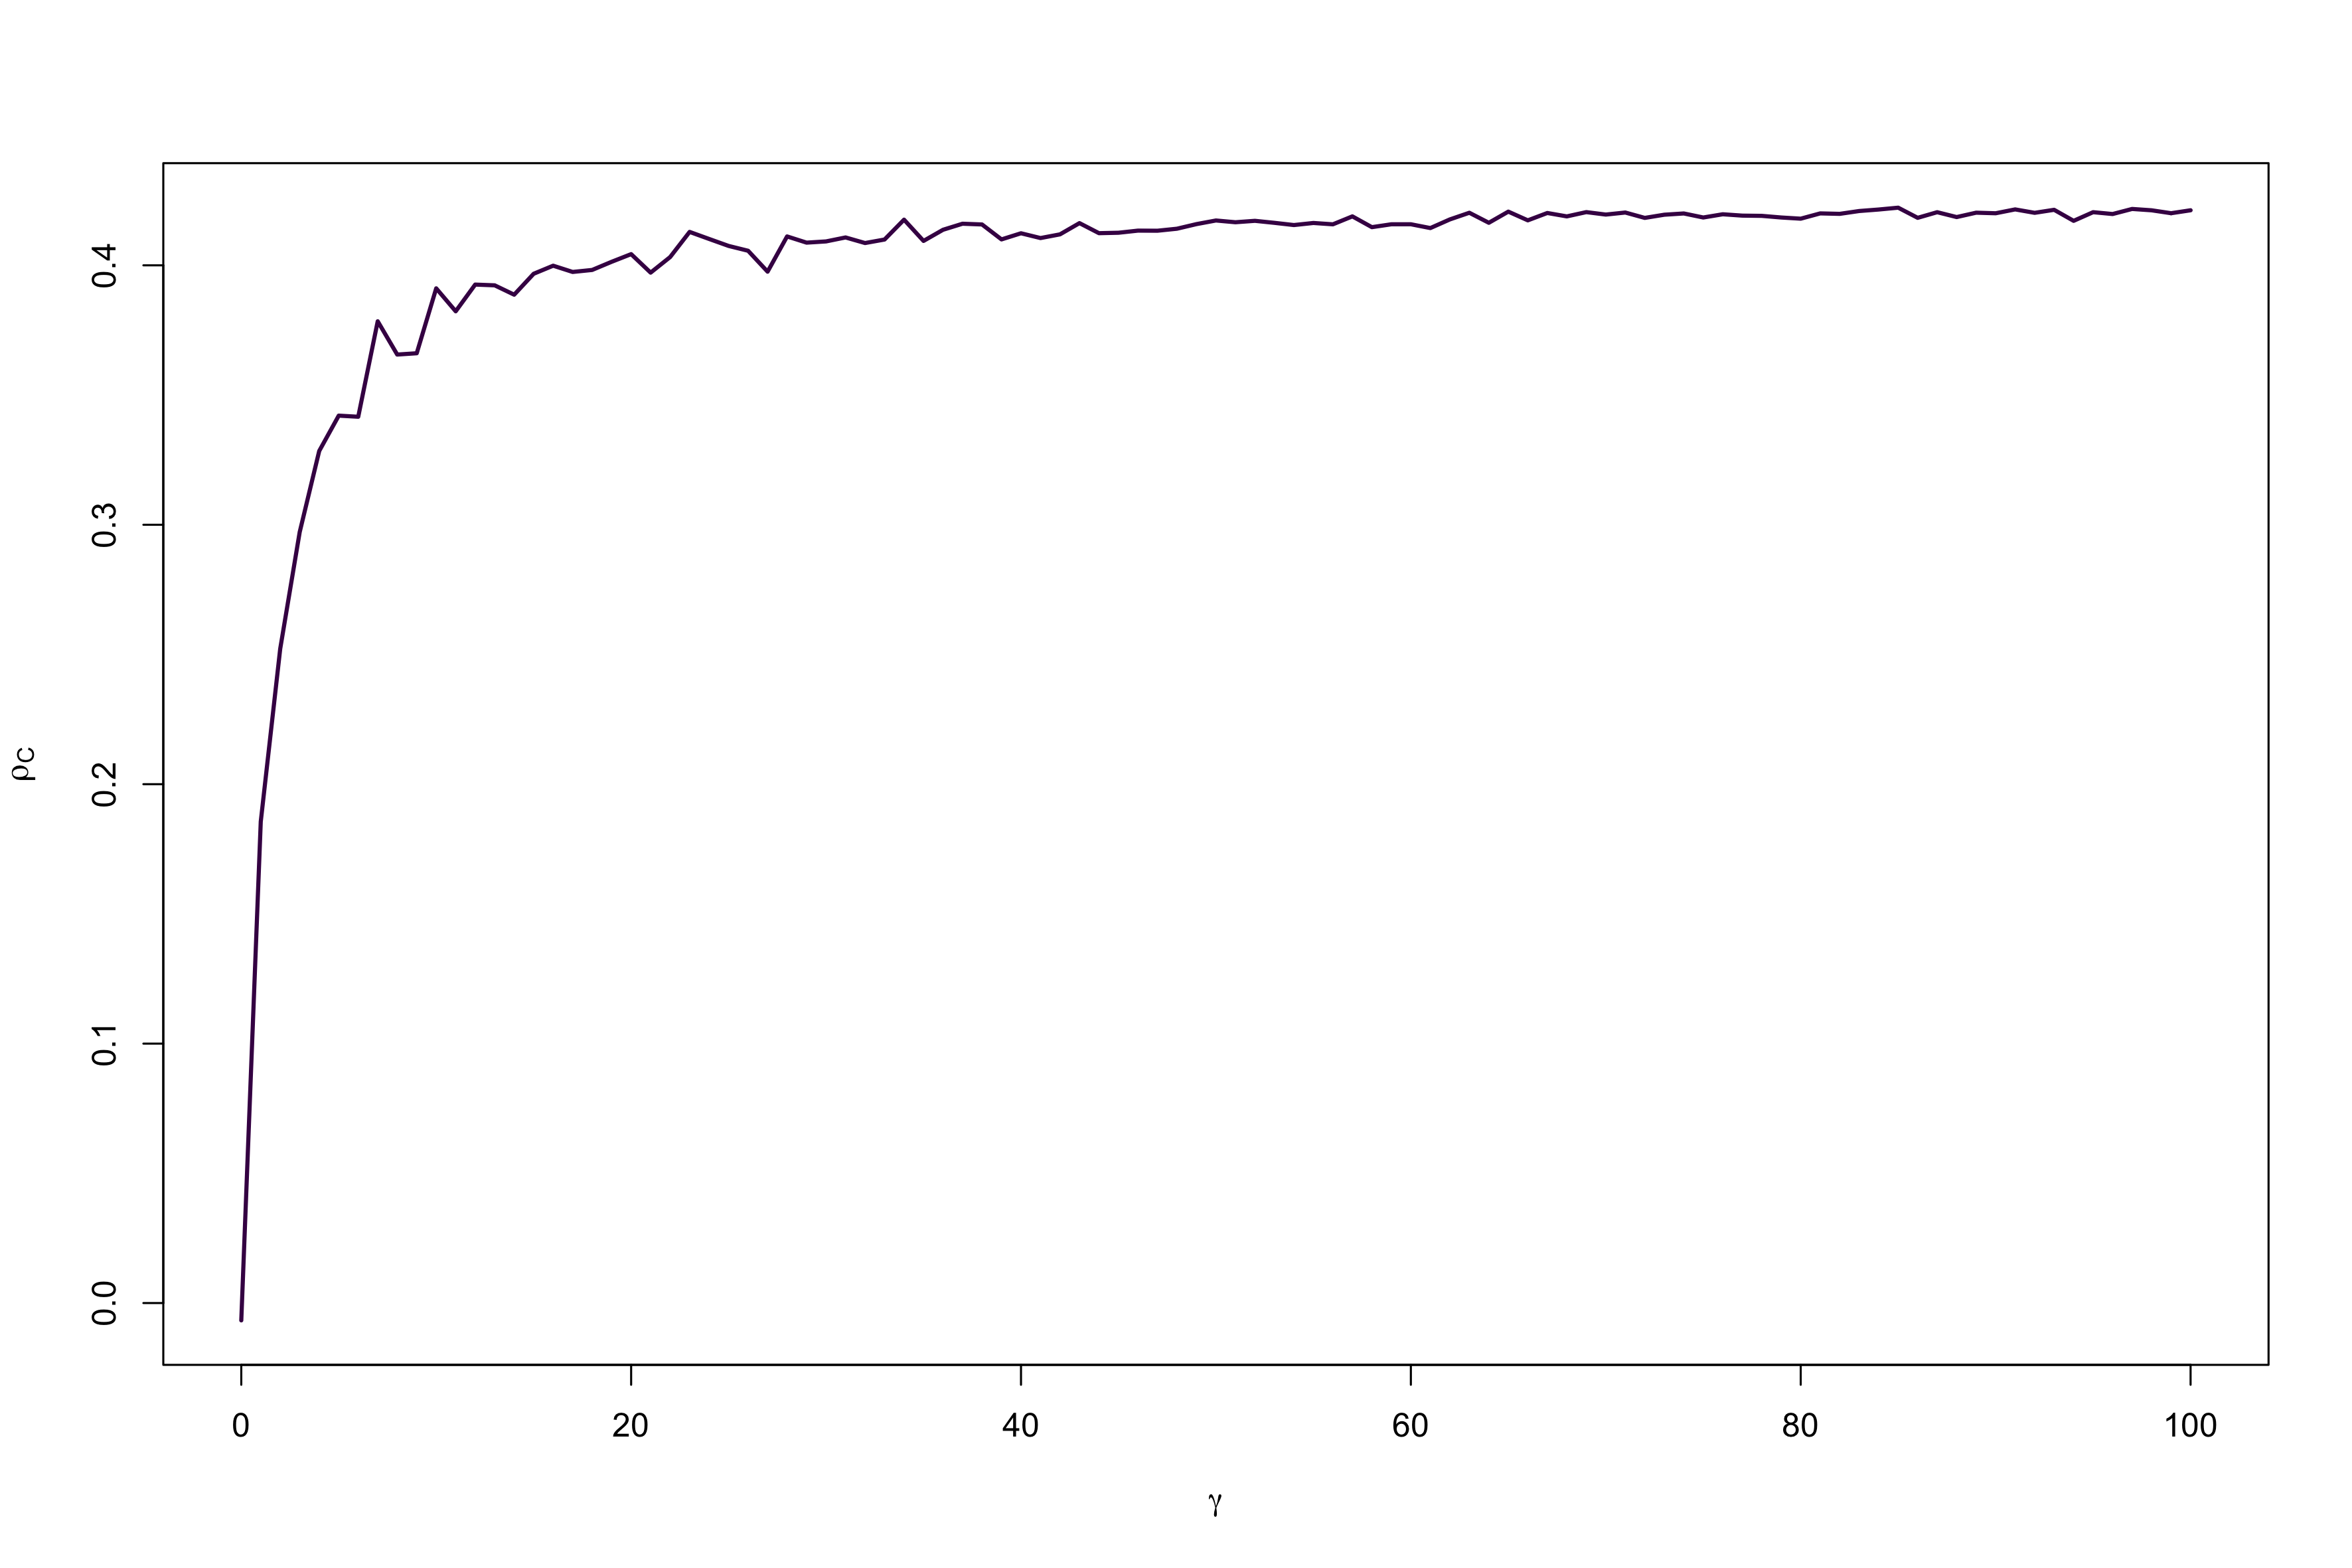
\includegraphics[width=10cm]{spearman_rho.png}
\caption{Gráfica de la rho de Spearman en función de gamma: $\uptau_C (\gamma)$.}
\label{fig:spearman_rho}
\end{figure}

\newpage

Por último, se presenta una gráfica de la cópula \eqref{copula_distribucion} y sus curvas de nivel para $\gamma = 5$. Para generar la gráfica de $C(u, v)$, se utiliza una muestra de $m(\omega_1, \omega_2)$ para $\gamma = 5$ y la expresión de $C$ como valor esperado para evaluar la función. En la figura \ref{fig:copula} se pueden notar gráficamente algunas de las propiedades de $C$, como que cae a cero cuando $u \to 0$ o $v \to 0$ y que $C (u, v) \to 1$ cuando $(u, v) \to (1, 1)$.

\begin{figure}[!htb]
    \centering
    \begin{subfigure}[t]{0.45\textwidth}
        \centering
        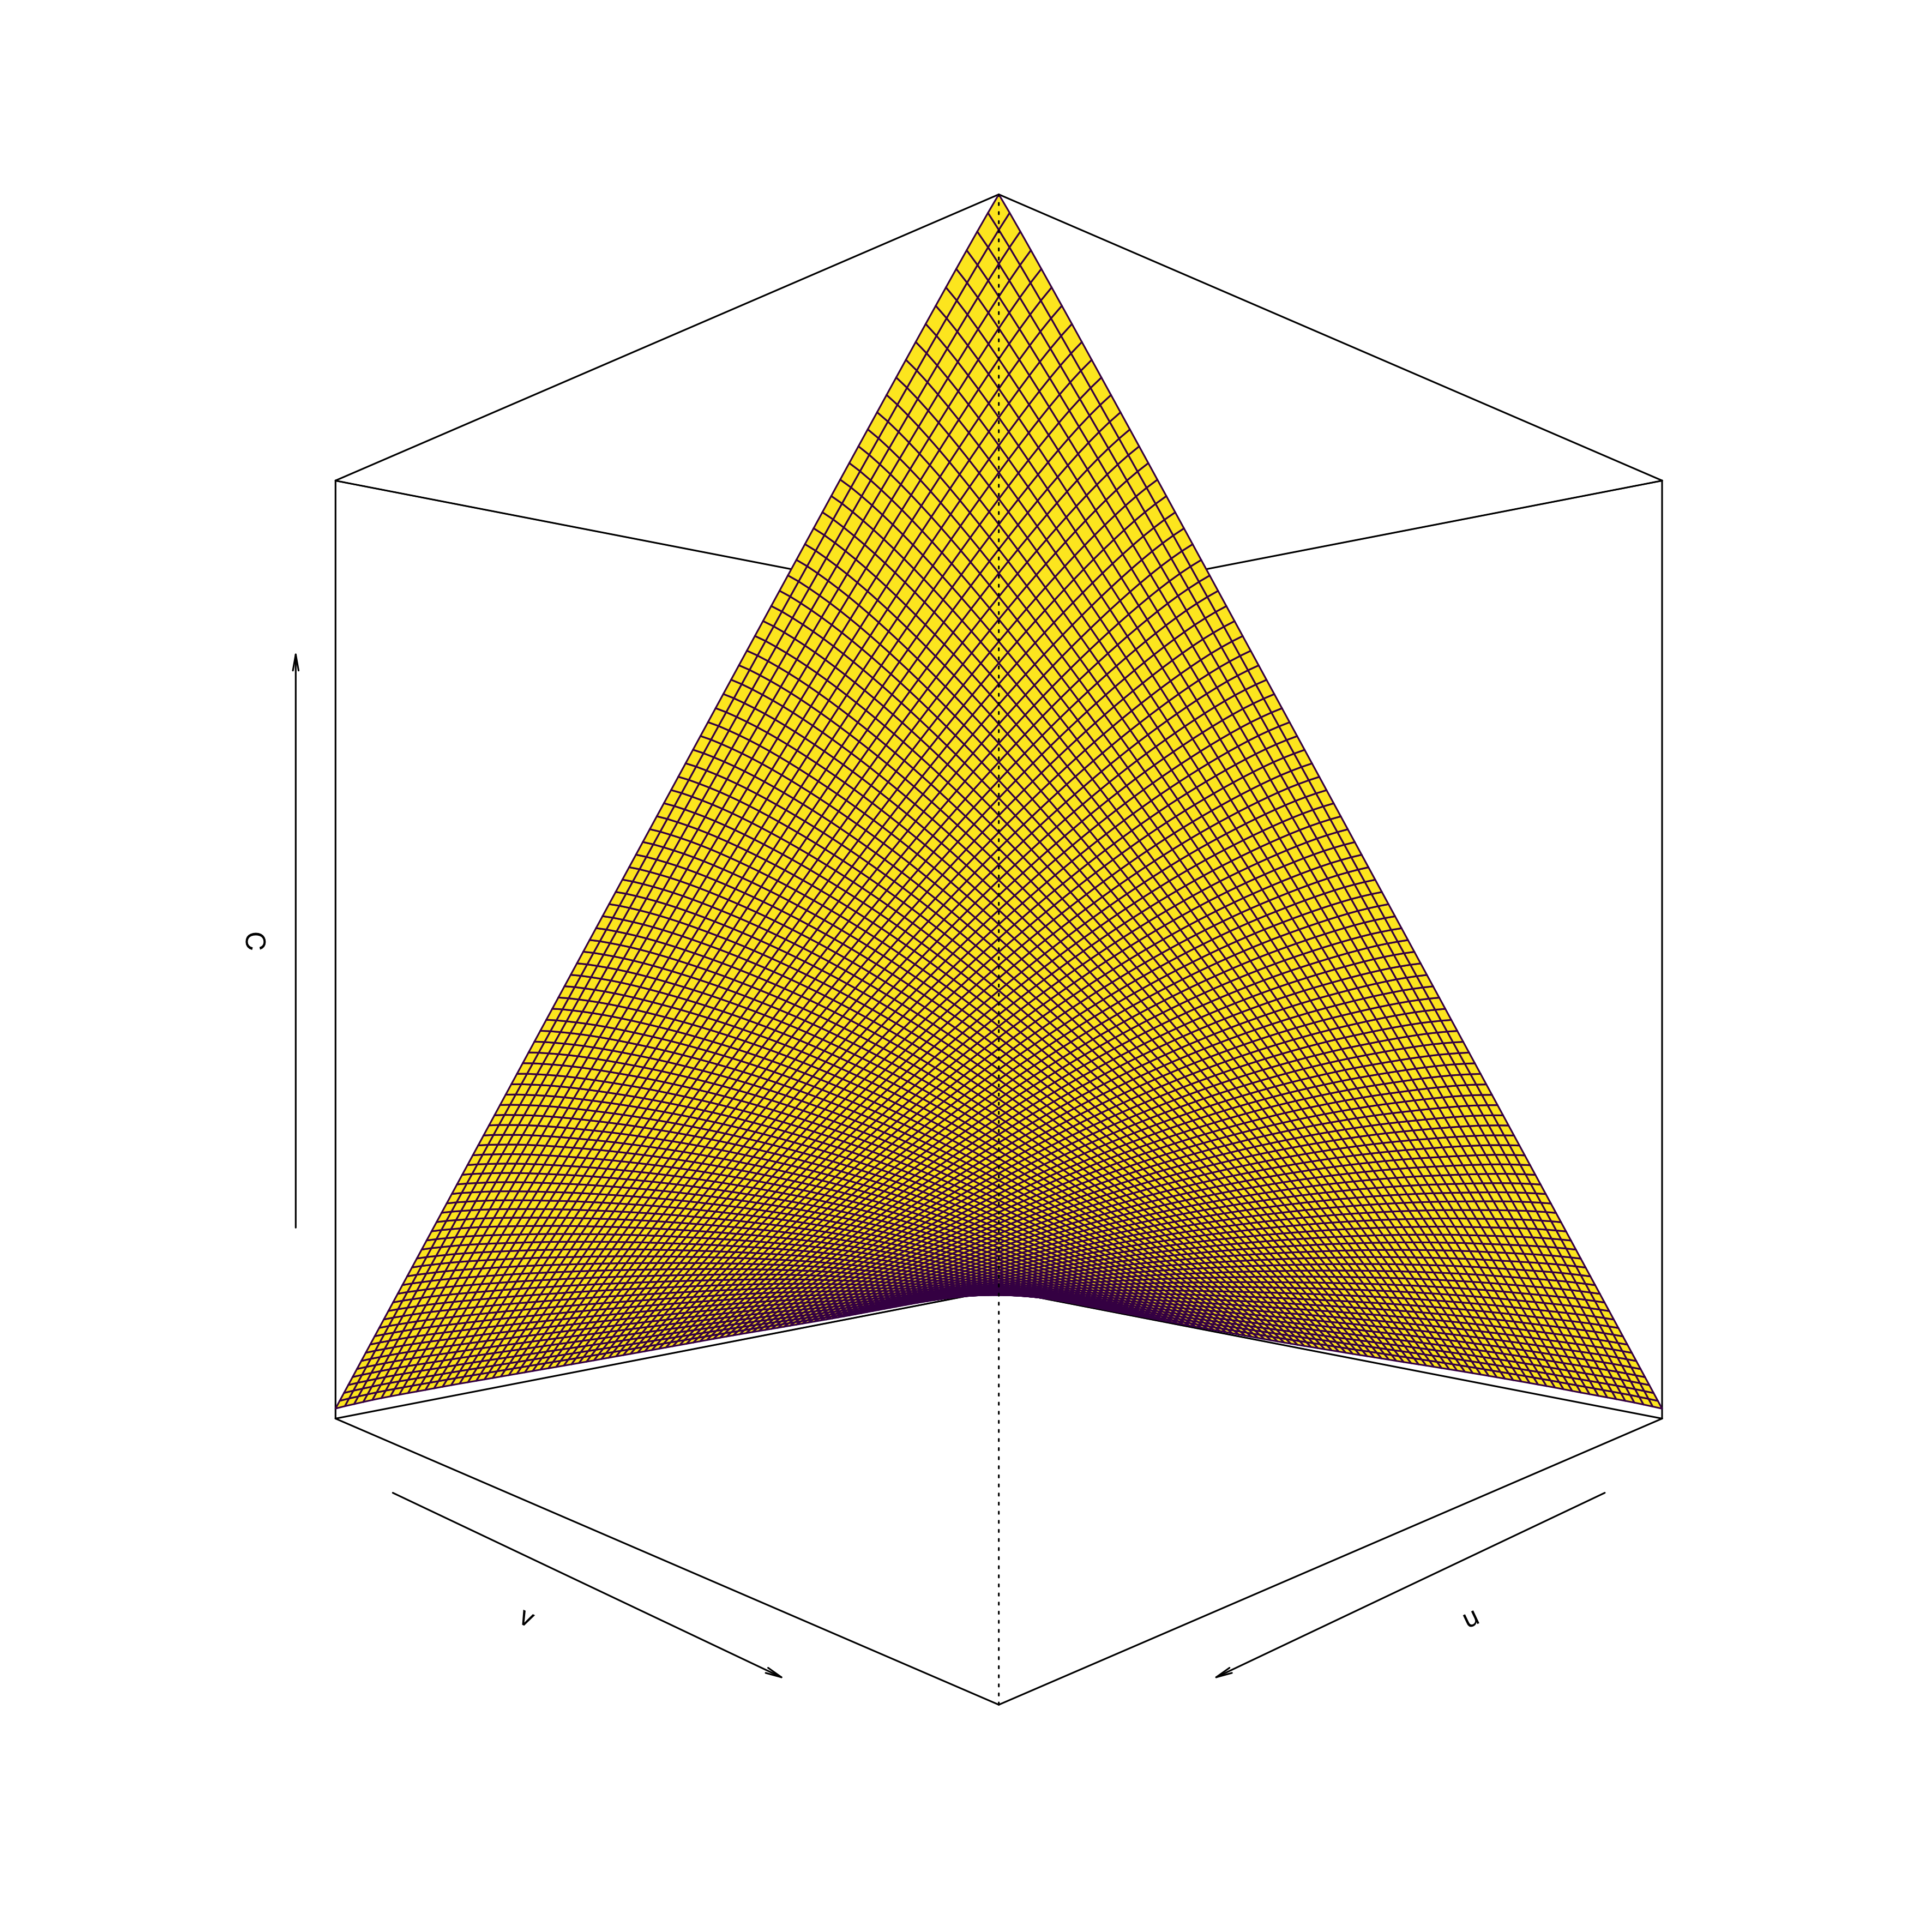
\includegraphics[width=\linewidth]{copula_5.png}
        \caption{$C(u, v)$ en el cubo $(u, v, C) \in [0, 1]^3$.}
        \label{fig:copula_3d}
    \end{subfigure}
    \hfill
    \begin{subfigure}[t]{0.45\textwidth}
        \centering
        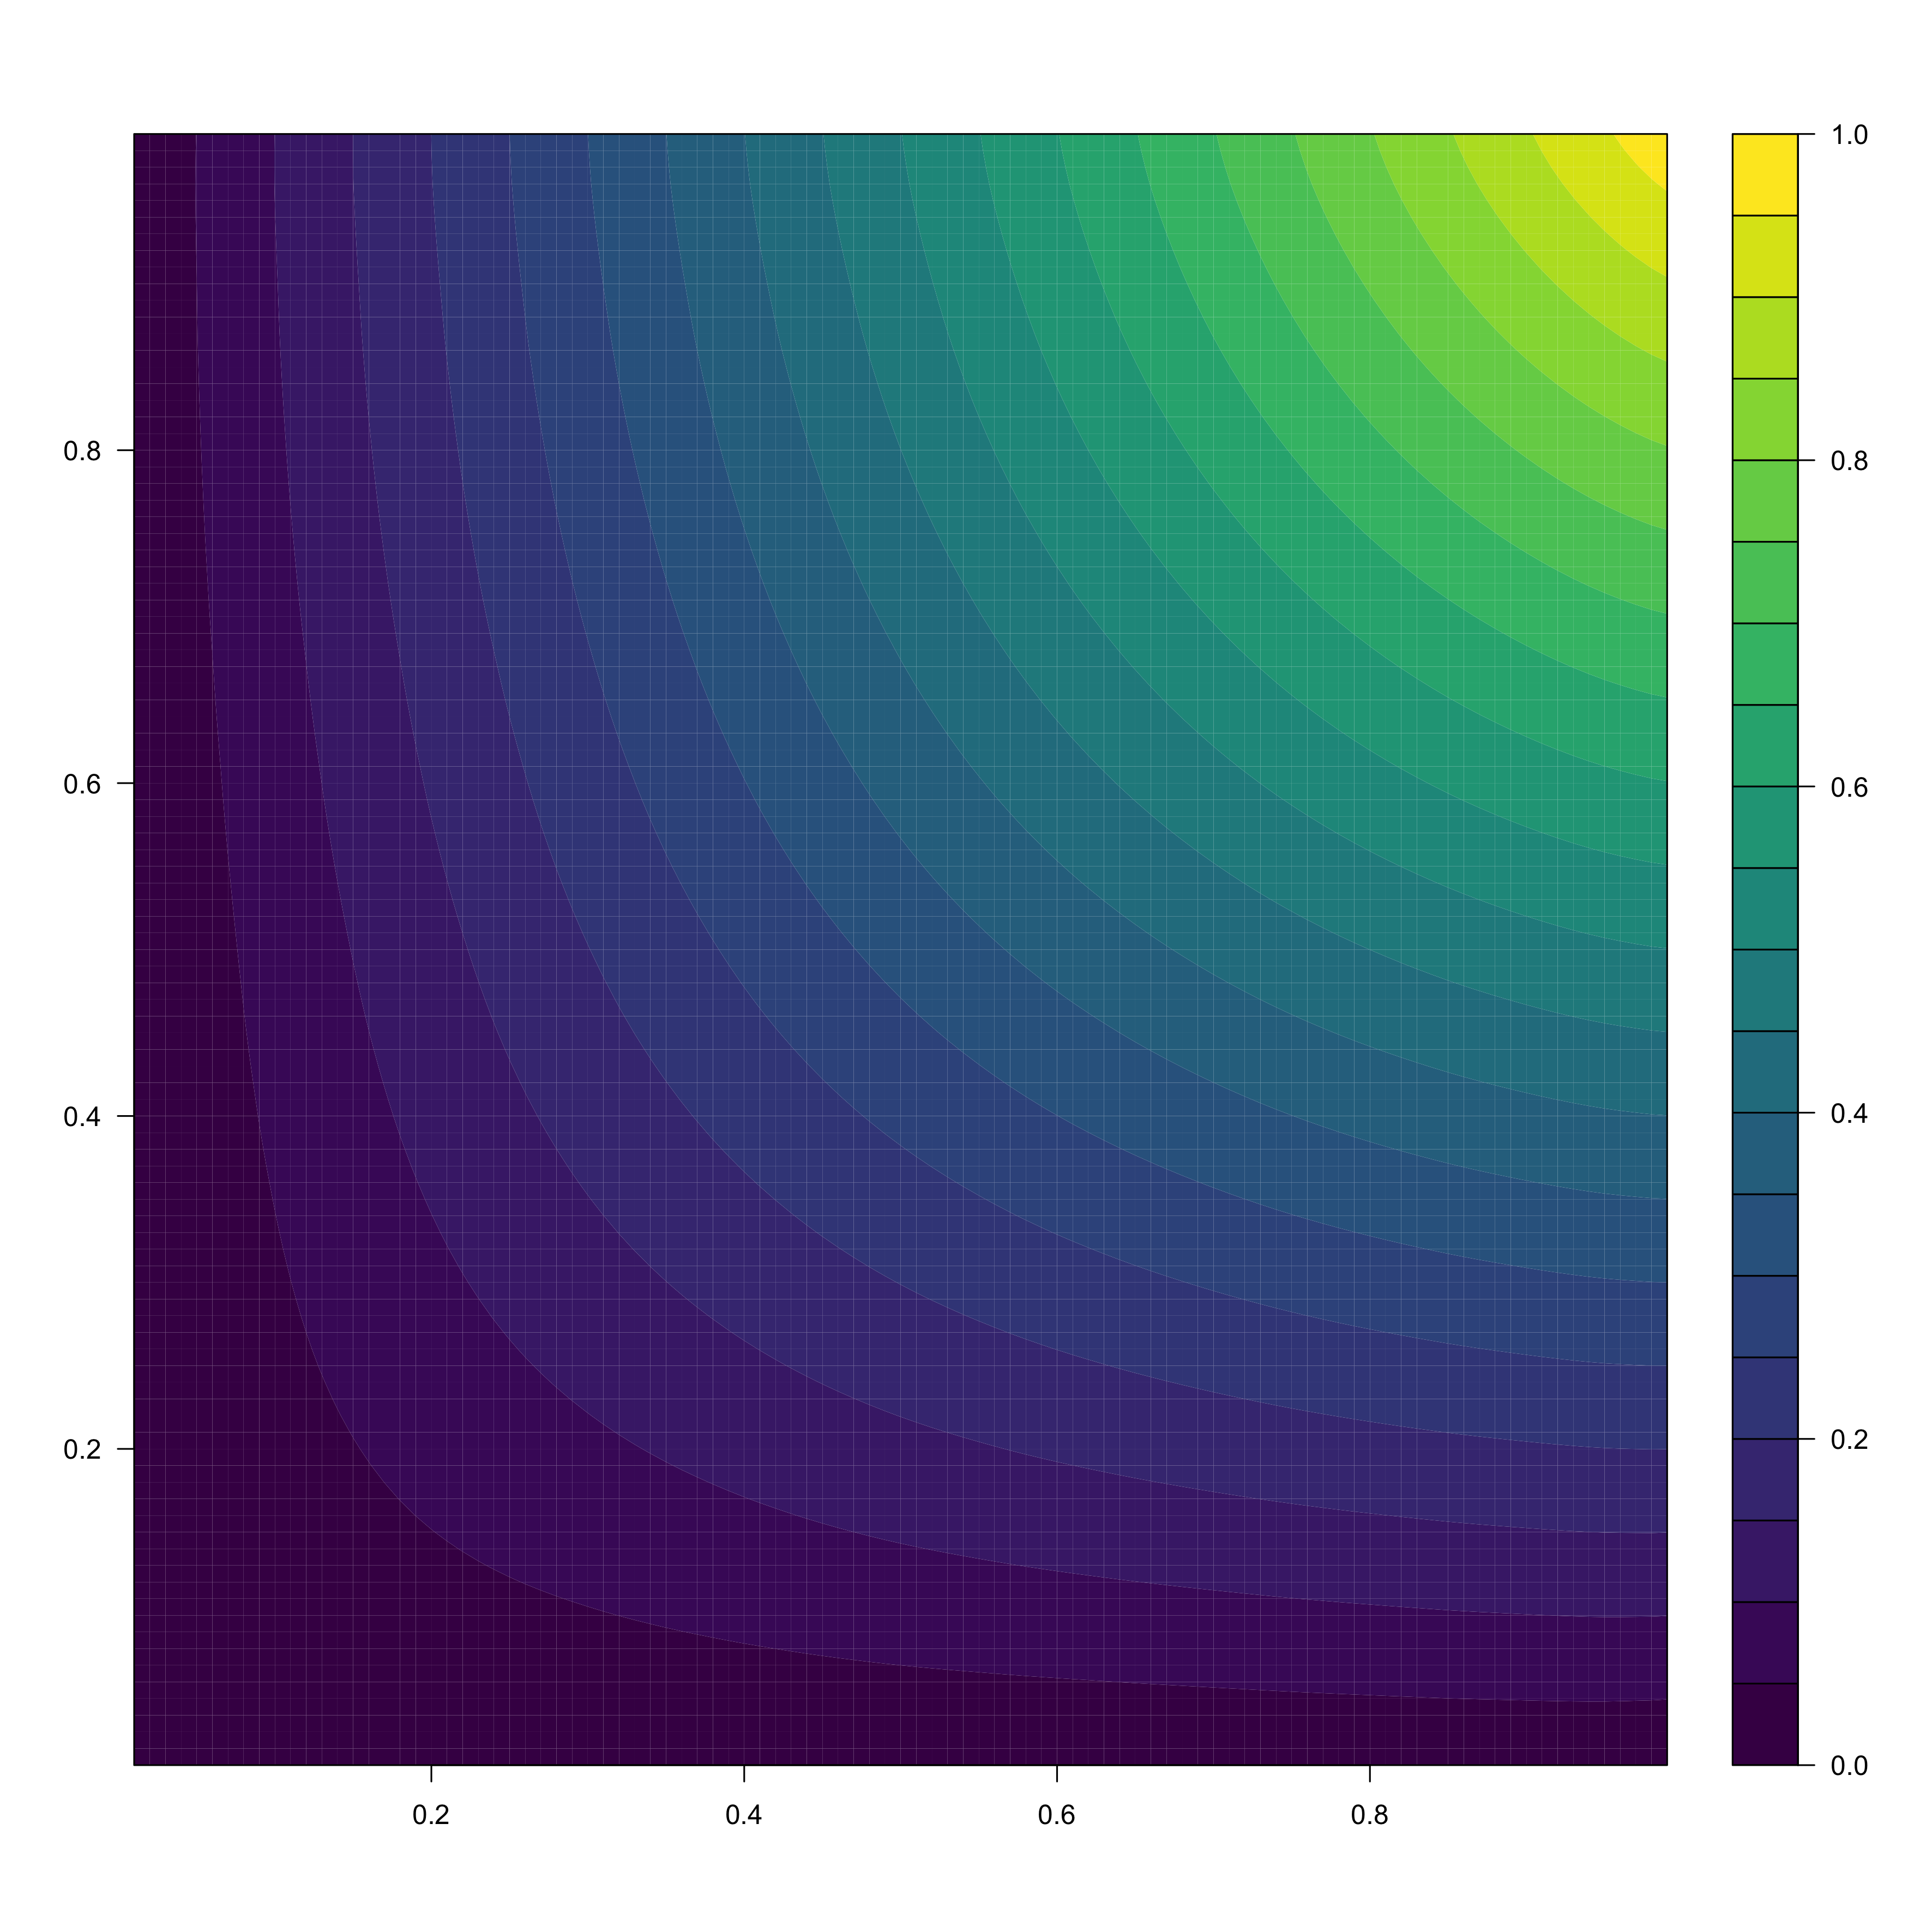
\includegraphics[width=\linewidth]{copula_5_contour.png} 
        \caption{Curvas de nivel de $C(u, v)$.}
        \label{fig:copula_contour}
    \end{subfigure}
    \caption{Gráfica y curvas de nivel de $C(u, v)$ para $\gamma = 5$.}
    \label{fig:copula}
\end{figure}

Ya que se formuló el modelo, se usarán modelos semiparamétricos para describir las tasas de riesgo $h_1$ y $h_2$. El mecanismo de inferencia es bayesiano por lo que se asignan distribuciones iniciales no paramétricas para $h_1$ y $h_2$ y una distribución paramétrica para el parámetro $\gamma$.  Adicional a esto, en el siguiente apartado se calculan las distribuciones posteriores condicionales de todos los parámetros y se explica cómo simular observaciones de ellas utilizando el muestreador de Gibbs. También se explica cómo incorporar las variables latentes $\omega_1$, $\omega_2$ y $y$ en las simulaciones para simplificar las simulaciones de los parámetros de interés.

\subsection{Distribuciones iniciales y posteriores}
\label{sec:ini_post}

Utilizando las ideas introducidas en \citet{old_nieto}, se define una distribución inicial no paramétrica para las funciones de riesgo utilizando procesos de Markov como sigue. Sea $0 = \uptau_0 < \uptau_1 < \dots$ una partición de la escala de tiempo. La tasa de riesgo $h_j(t)$ $(j = 1, 2)$ está dada por $$h_j(t) = \sum_{k=1}^\infty \lambda_{jk} \mathbb{I}\lbrace \uptau_{k-1} < t \leq \uptau_{k} \rbrace,$$ y se define a través de un proceso latente $\lbrace u_{jk} \rbrace$ y el proceso estacionario $\lbrace \lambda_{jk} \rbrace$ de la siguiente manera:
\begin{align}
\lambda_{j1} &\sim Ga(\alpha, \beta),\label{eq:lambda1}\\
u_{jk} | \lambda_{jk} &\sim Po(c_{jk}\lambda_{jk}) \text{ para } k = 1, 2, \dots,\label{eq:uk}\\
\lambda_{j,k+1}|u_{jk} &\sim Ga(\alpha + u_{jk}, \beta + c_{jk}) \text{ para } k = 1, 2, \dots.\label{eq:lambdak1}
\end{align}
Las ecuaciones \eqref{eq:lambda1} a \eqref{eq:lambdak1} implican que marginalmente $\lambda_{jk} \sim Ga(\alpha, \beta)$ y se tiene una estructura de dependencia caracterizada por $$cor(\lambda_{jk}, \lambda_{j,k+1}) = \frac{c_{jk}}{c_{jk} + \beta}.$$ Más aún, si $c_{jk} = 0$ se tiene que las $\lambda_{jk}$'s son independientes.

Ahora se obtiene la forma de la distribución posterior. Sea $T_{(n)}$ una muestra de tamaño $n$ del vector aleatorio $T=(T_1, T_2)$ con función de densidad $f(t_1, t_2)$. Para simplificar la notación, se omite la dependencia del parámetro $h = (h_1, h_2).$ La función de densidad conjunta de $T$ y el vector de variables latentes $\omega$ está dada por $$f(t_1, t_2, \omega_1, \omega_2) = f_1(t_1|\omega_1)f_2(t_2|\omega_2)m(\omega_1, \omega_2).$$ De la construcción \eqref{eq_omegas} se tiene que la distribución de $\omega$ depende de la variable latente $y$ por lo que, considerando la independencia condicional de $\omega_1$ y $\omega_2$ dado $y$, se puede extender esta densidad conjunta para obtener
$$f(t_1, t_2, \omega_1, \omega_2, y)= f_1(t_1|\omega_1)f_2(t_2|\omega_2)m(\omega_1|y)m(\omega_2|y)g(y).$$ Se puede evitar la marginalización sobre $\omega$ y $y$ trabajando como si estas dos variables fueran observadas junto con $T$. Así, cada observación $(t_{i1}, t_{i2})$ del vector $T$ necesita del vector de variables latentes $(\omega_{i1}, \omega_{i2}, y_i)$. Si la muestra consiste únicamente de observaciones exactas, la función de verosimilitud está dada por 
$$\mathcal{L}(t, \omega, y | h) = \prod_{i=1}^n f_1(t_{i1}|\omega_{i1})f_2(t_{i2}|\omega_{i2})m(\omega_{i1}|y_i)m(\omega_{i2}|y_i)g(y_i).$$

Se utiliza el teorema de Bayes para obtener la distribución posterior de $h$, la cual es proporcional al producto de la verosimilitud y la distribución inicial $$\pi(h | t, \omega, y) \propto \mathcal{L}(t, \omega, y | h) \pi(h).$$ La distribución inicial de $h_j$ es la distribución conjunta de las componentes del vector $\lambda_j$ $(j = 1, 2)$. Para escribir explícitamente la inicial $\pi(h_j)$ se considera la densidad conjunta de los vectores $\lambda_j$ y $u_j$. Por facilidad se omite el subíndice $j$ de ambos vectores. Se tiene que
\begin{align}
\label{eq:inicial_ext}
    \pi(\lambda, u) &= \pi(\lambda_1) \prod_{k = 2}^\infty \pi(\lambda_k | u_{k-1})\pi(u_{k-1}|\lambda_{k-1})\\
    & = Ga(\lambda_1 | \alpha, \beta) \prod_{k = 2}^\infty Ga(\lambda_k | \alpha + u_{k-1}, \beta + c_k) Po(c_k\lambda_{k-1}).\nonumber
\end{align}
Se puede evitar la marginalización sobre las componentes del vector $u$ al trabajar con la distribución conjunta de $(\lambda, u)$ e incluir a $u$ en el proceso inferencial. De esta manera, sustituyendo la distribución incial $\pi(h_j)$ por la distribución conjunta de la ecuación \eqref{eq:inicial_ext}, se tiene que la distribución posterior de $h = (h_1, h_2)$ si la muestra consiste únicamente de observaciones exactas está dada por
\begin{align*}
    \pi(h | t, \omega, y) &\propto \mathcal{L}(t, \omega, y | h) \prod_{j = 1}^2 \pi(\lambda_j, u_j)\\
    &\propto \prod_{i=1}^n f_1(t_{i1}|\omega_{i1})f_2(t_{i2}|\omega_{i2})m(\omega_{i1}|y_i)m(\omega_{i2}|y_i)g(y_i)\times \\
    &\ \ \ \ \prod_{j = 1}^2 \left(\pi(\lambda_{j1})\prod_{k = 2}^\infty \pi(\lambda_{jk} | u_{j,k-1})\pi(u_{j,k-1}|\lambda_{j,k-1})\right)
\end{align*}

Las variables $\omega$ y $y$ no son observadas por lo que, para simular observaciones de la distribución posterior de $h$ utilizando el muestreador de Gibbs, se necesitan las expresiones para las distribuciones posteriores condicionales de $\omega, y, \lambda$ y $u$ que se calculan a continuación.

\subsubsection*{Variables latentes $\omega_{ij}$}
\label{posterior_omega}

La distribución posterior condicional de $\omega_{ij}$ es de la forma
\begin{align*}
m(\omega_{ij} | t, y, h) &\propto p(t, y, h, \omega)\\
&\propto \mathcal{L}(t, \omega, y |h) \pi(h)\\
&\propto \mathcal{L}(t, \omega, y |h)\\
&\propto f_j(t_{ij}|\omega_{ij})m(\omega_{ij}|y_i)\\
&\propto \frac{h_j(t_{ij})}{\omega_{ij}}\mathbb{I}\lbrace \omega_{ij} > H_j(t_{ij})\rbrace \  \omega_{ij}^{1+y_i} \ \exp (-(1+\gamma)\omega_{ij})\\
&\propto \omega_{ij}^{y_i} \ e^{-(1+\gamma)\omega_{ij}} \ \mathbb{I}\lbrace \omega_{ij} > H_j(t_{ij})\rbrace.
\end{align*}

La forma funcional se asemeja a una distribución Gamma, pero la restricción sobre el dominio de $\omega_{ij}$ trunca esta distribución. Para simular una observación de esta distribución en el paso $(t+1)$ se utiliza el algoritmo de Metropolis-Hastings. Como distribución candidata se analizaron dos opciones. Primero, se utilizó una distribución gamma trasladada, independiente de $\omega_{ij}^{(t)}$, de la forma $$f_1 \sim Ga(1 + y_i^{(t)}, 1 + \gamma^{(t)}) + H_j(t_{ij})^{(t)}.$$ La segunda opción fue una distribución uniforme de la forma $$f_2 \sim U(\max \lbrace H_j(t_{ij})^{(t)}, \ \omega_{ij}^{(t)} - a \rbrace, \ \omega_{ij}^{(t)} + a),$$ donde $a$ es una constante positiva.

Realizando algunos experimentos con ambas opciones, se utilizó finalmente la distribución uniforme. Esto se debe a que las propuestas independientes de la gamma trasladada tienden a rechazar más propuestas que la distribución uniforme y la cadena se ``atora" más. Como ejemplo se incluye la simulación de una cadena con cada propuesta, para los valores fijos $a = 3$, $\gamma = 1$ y $H_j(t_{ij}) = 0.9$ en las figuras \ref{fig:prop_gamma} y \ref{fig:prop_unif}. Se puede ver que la figura \ref{fig:prop_unif} tiene menos espacios en blanco, que son pedazos en donde la cadena se atora. Además, parece que con las propuestas uniformes la cadena explora más valores del soporte que con las propuestas gamma independientes.

\begin{figure}[!htb]
\centering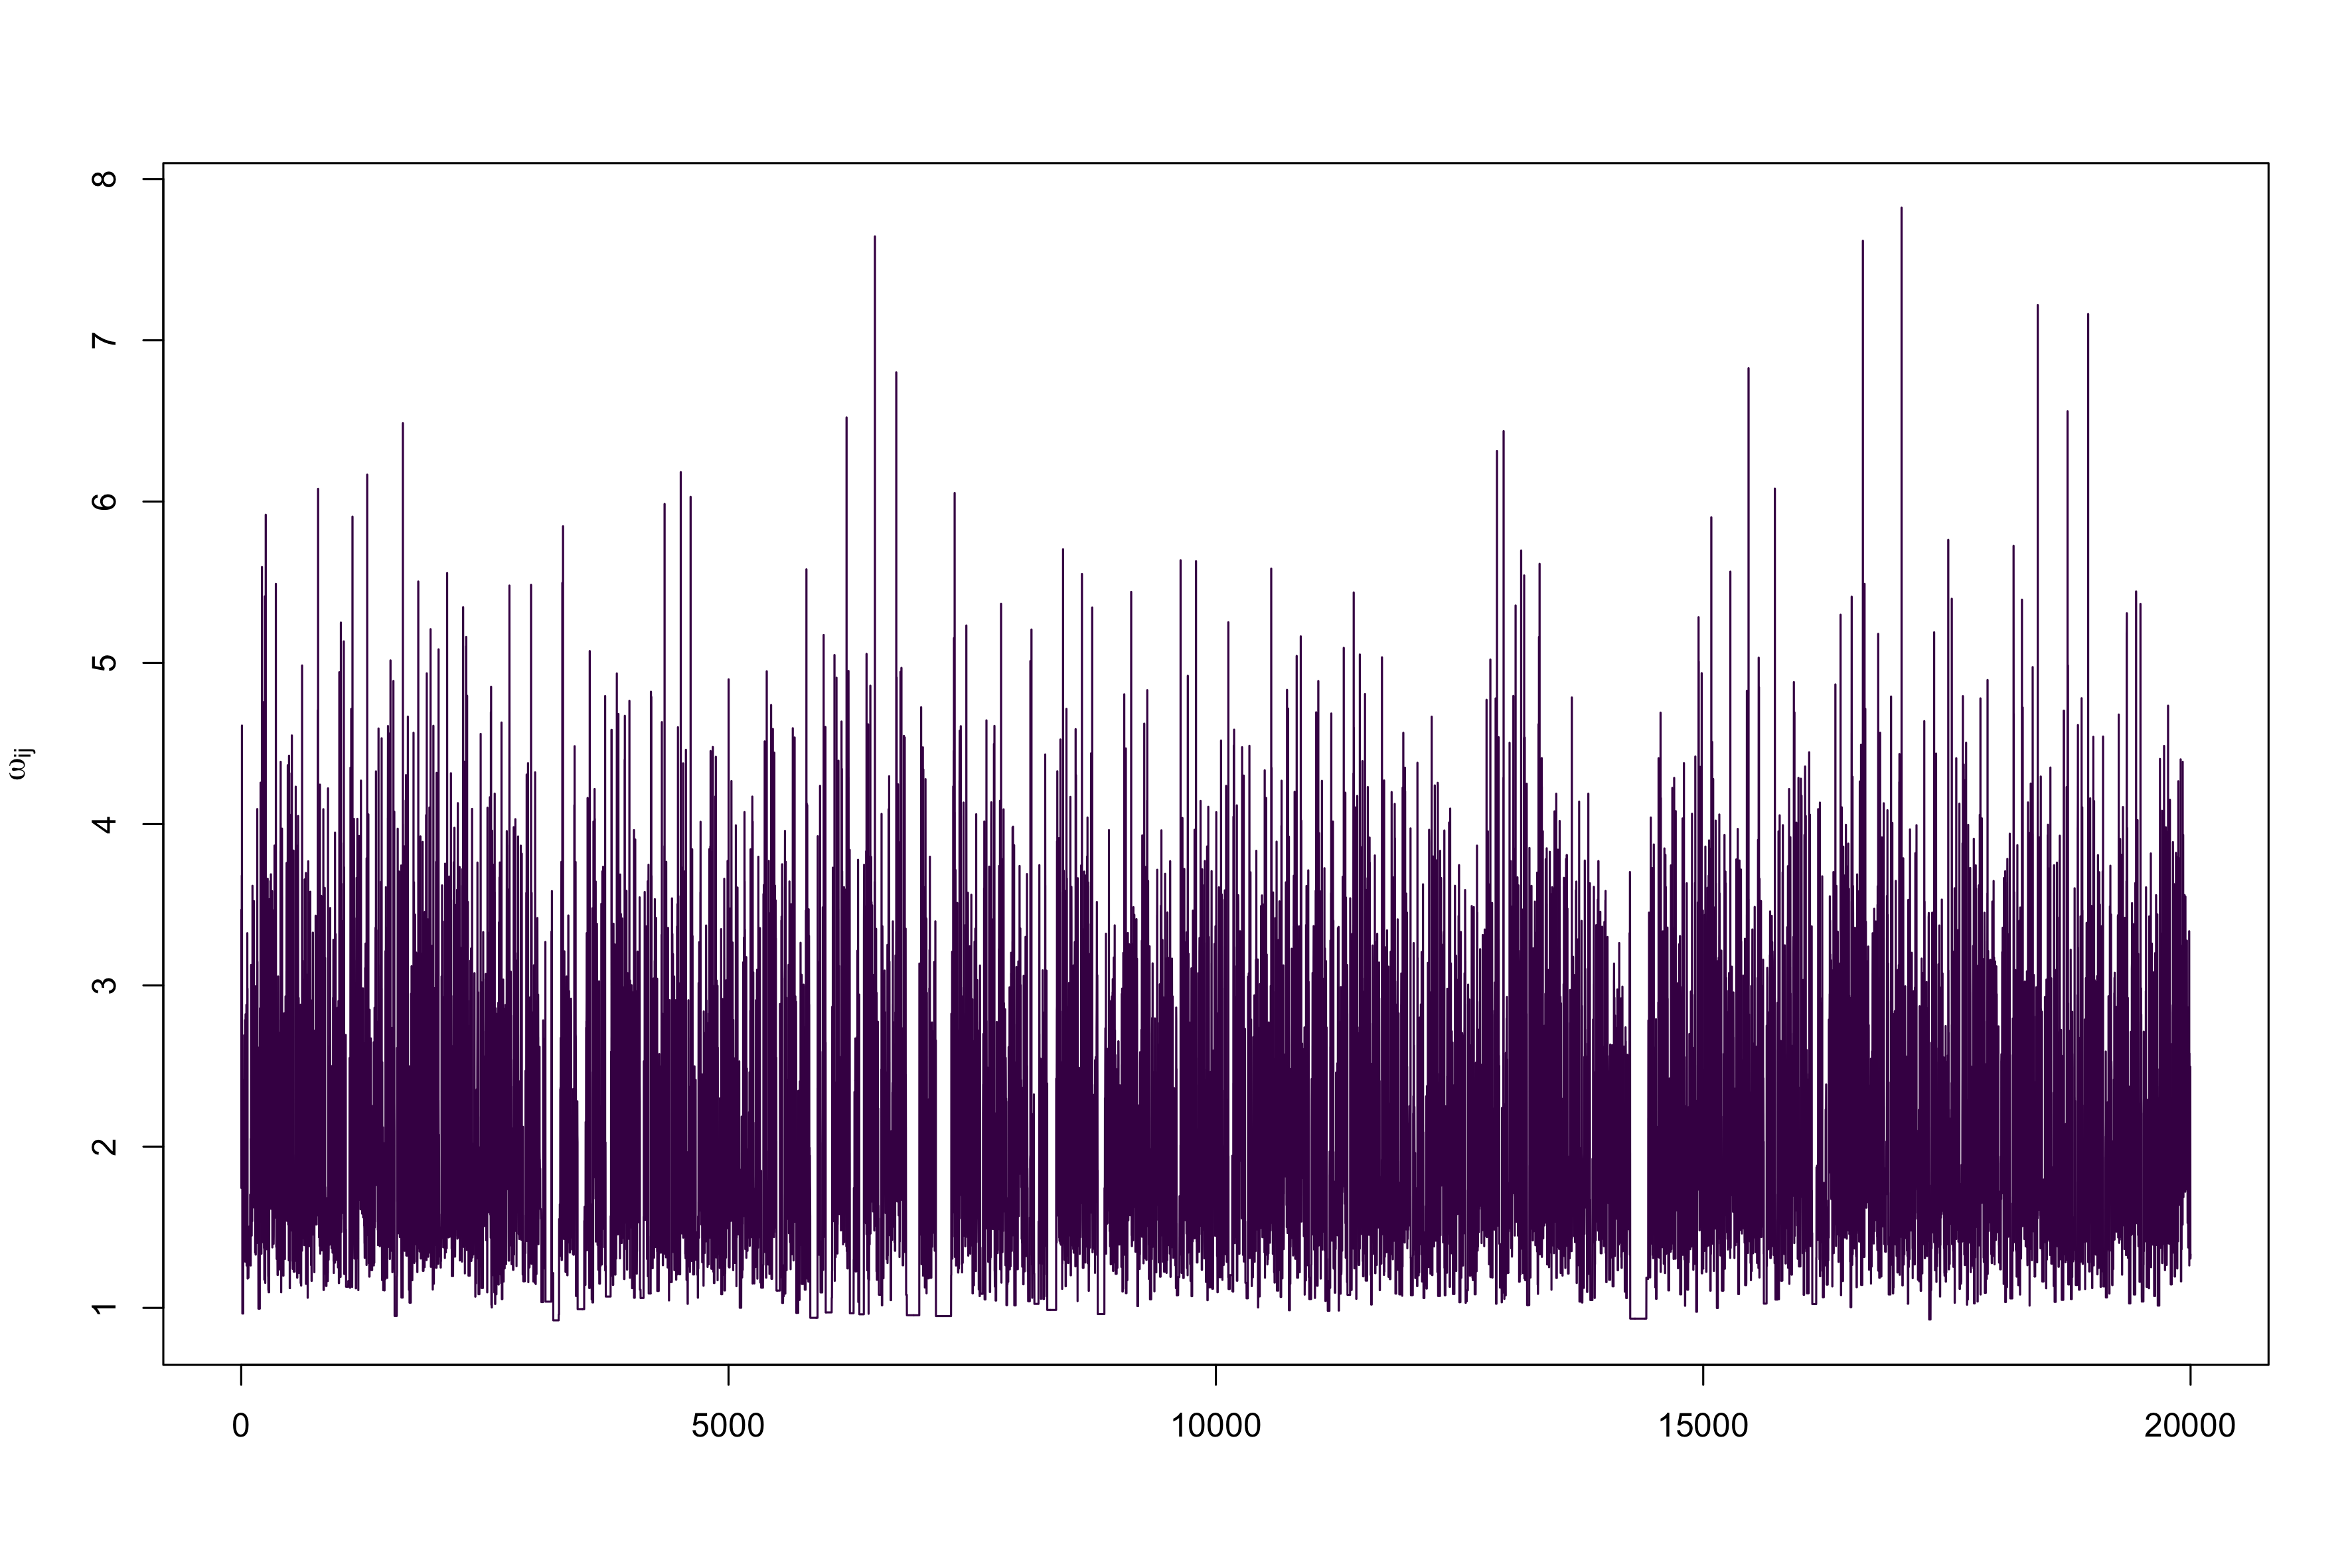
\includegraphics[width=10cm]{propuesta_gamma.png}
\caption{Cadena de Markov para $\omega_{ij}$ con propuestas $f_1$.}
\label{fig:prop_gamma}
\end{figure}

\begin{figure}[!htb]
\centering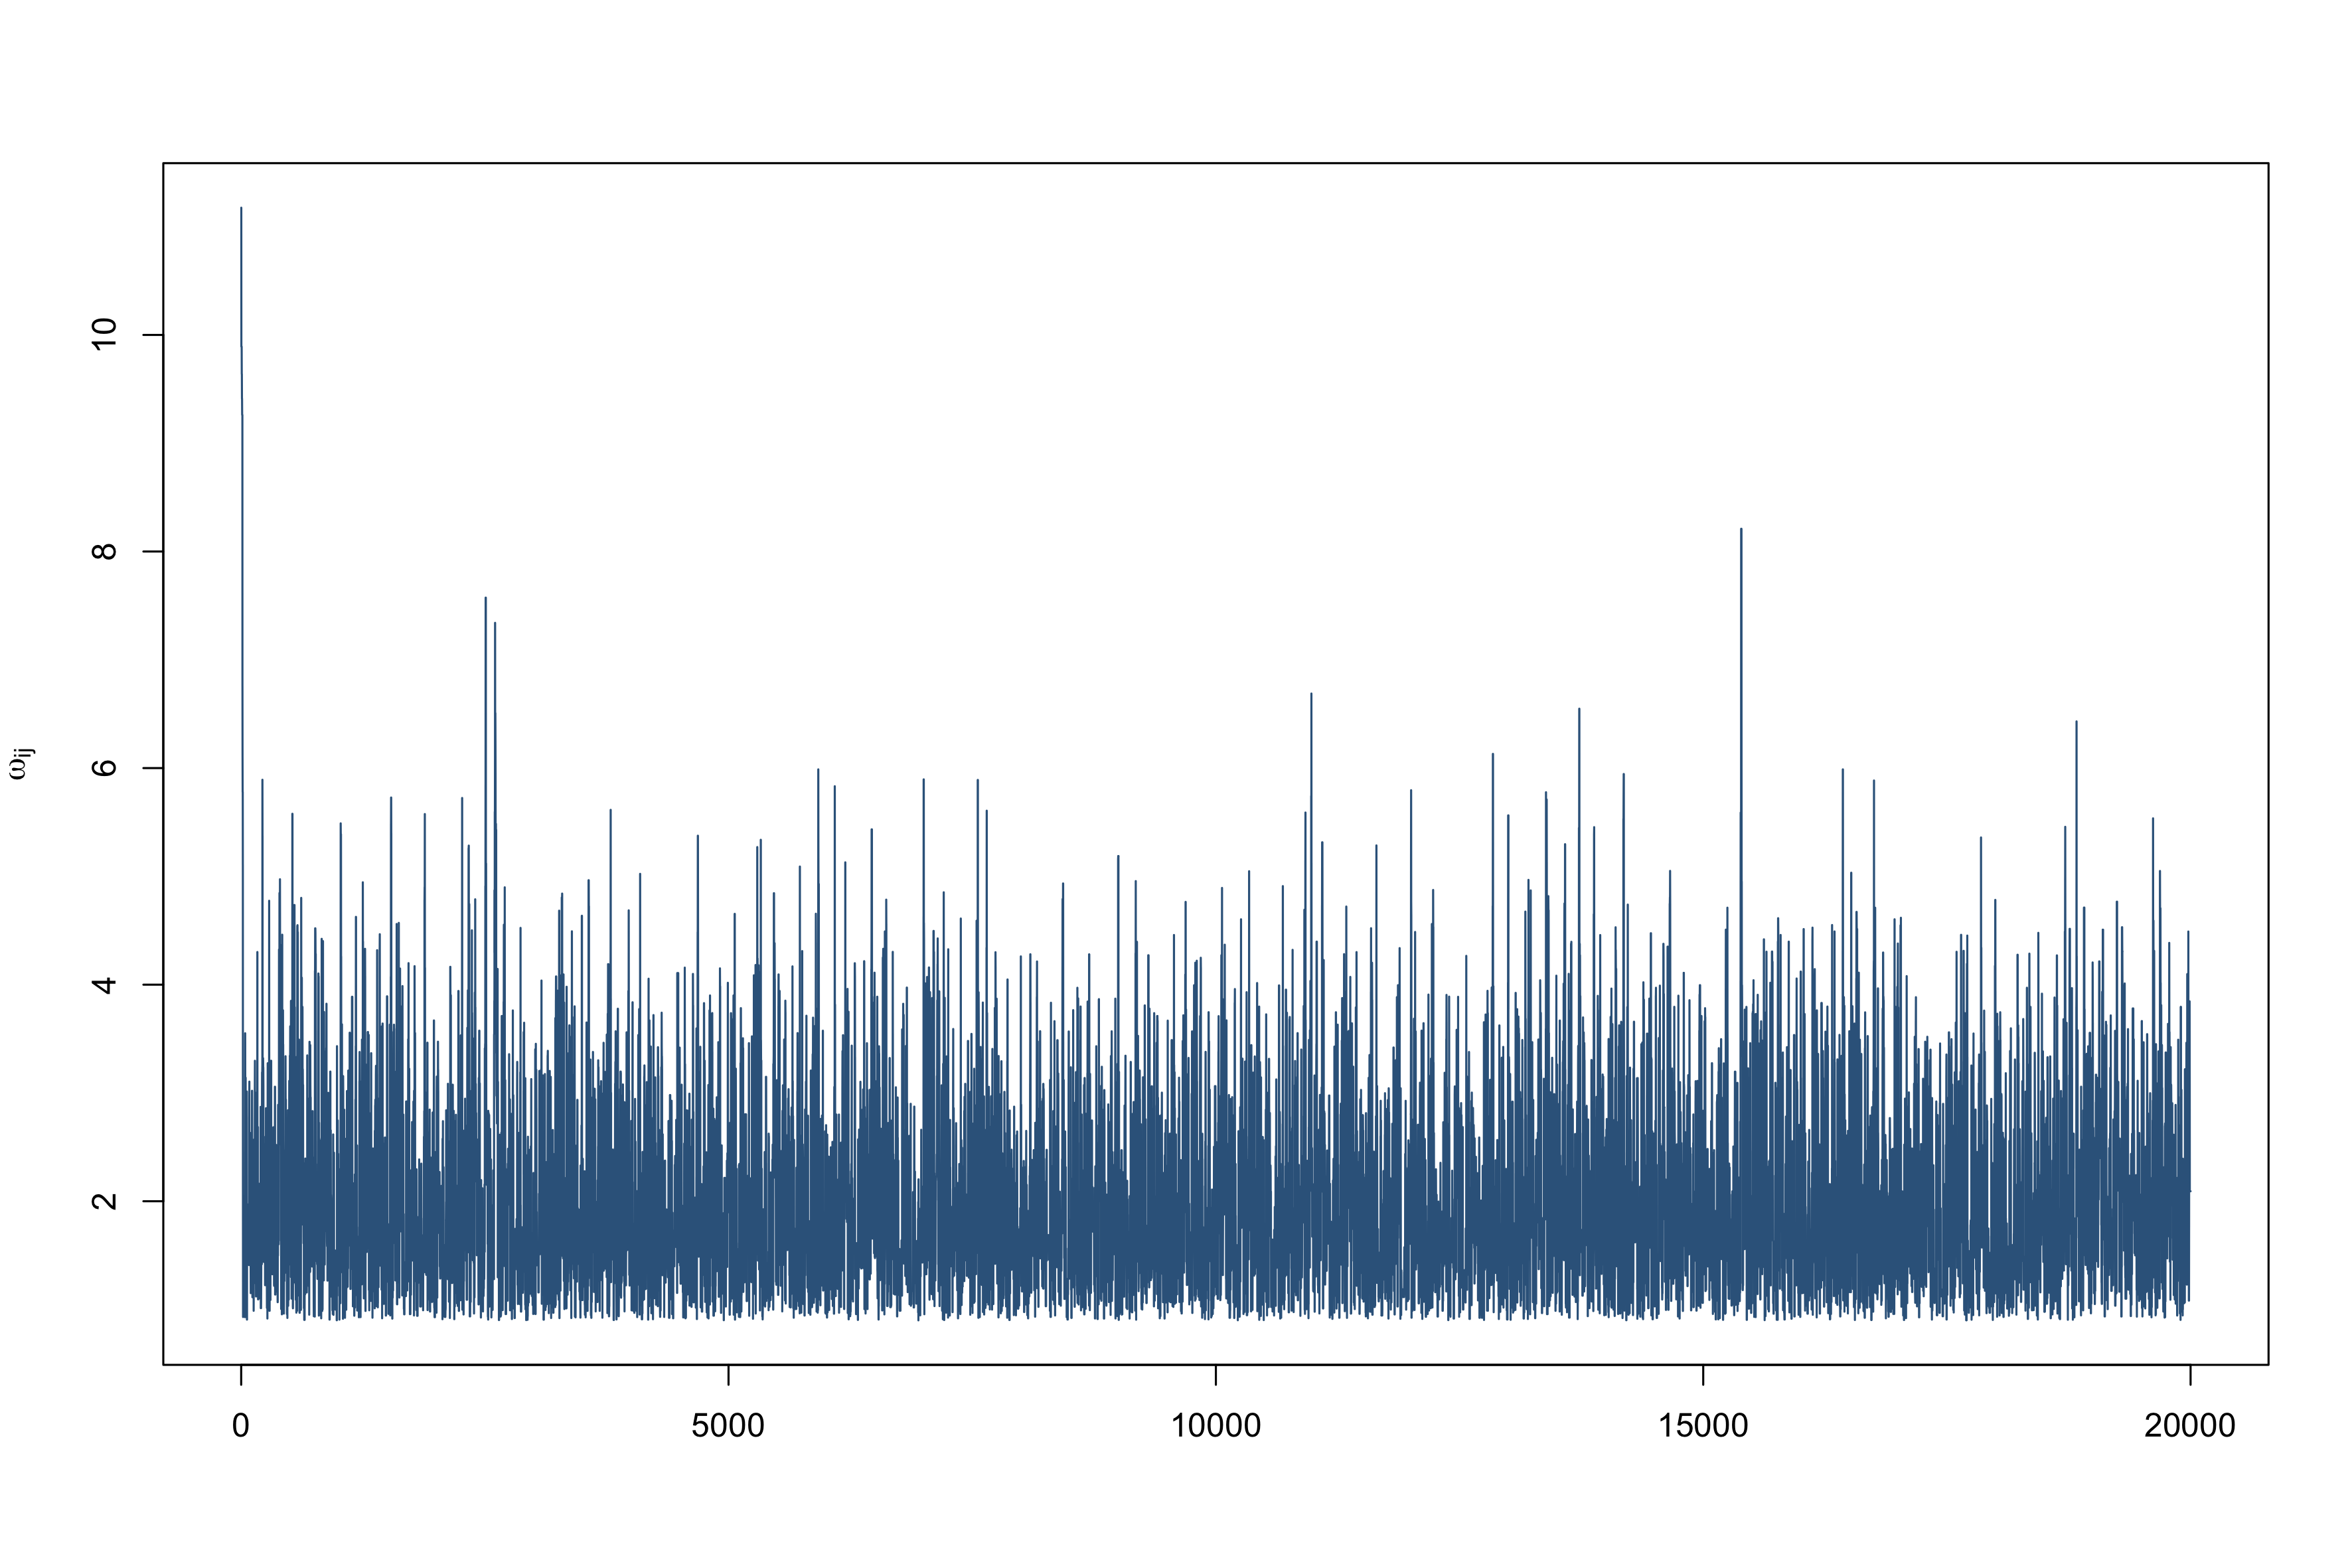
\includegraphics[width=10cm]{propuesta_uniforme.png}
\caption{Cadena de Markov para $\omega_{ij}$ con propuestas $f_2$.}
\label{fig:prop_unif}
\end{figure}

Para programar el paso de Metropolis-Hastings se debe calcular la razón de Hastings. Se denota $\omega^*$ a la observación candidata. Se puede verificar que el cociente de la densidad candidata $f_2(\omega_{ij} ^{(t)} | \omega^*)/f_2(\omega^* | \omega_{ij} ^{(t)})$ siempre es igual a 1, por lo que no es necesario incorporarlo en la razón. Entonces el logaritmo de la razón de Hastings queda de la siguiente forma:
\begin{align*}
\log (r(\omega_{ij}^{(t)}, \omega^*)) &= \log \left(\frac{m(\omega^* | y_i, \gamma)}{m(\omega_{ij}^{(t)}| y_i, \gamma)}\right)\\
&= y_i \left(\log (\omega^*) - \log (\omega_{ij}^{(t)})\right) - (1 + \gamma)(\omega^* - \omega_{ij}^{(t)}).
\end{align*}
El código para simular una observación del vector $\omega_j$ con propuesta uniforme se presenta en el cuadro \ref{cod:sim_omega}.
\newpage

\begin{table}[!htb]
\begin{lstlisting}
  sample_omega <- function(omega, y, cum_h, x, theta, gamma, omega_d = NULL) {

  if (is.null(omega_d)) omega_d <- y + 1

  bound <- cum_h * exp(x %*% theta)
  l1 <- max(bound, omega - omega_d)
  l2 <- omega + omega_d
  proposal <- stats::runif(n = 1, min = min(l1, l2), max = max(l1, l2))

  if (omega <= bound) {
    omega_out <- proposal
    return(omega_out)
  }

  log_alpha <-
    y * (log(proposal) - log(omega)) - (1 + gamma) * (proposal - omega)
  prob <- min(exp(log_alpha), 1)
  u <- stats::runif(n = 1)
  omega_out <- omega + (proposal - omega) * (u <= prob)

}
\end{lstlisting}
\caption{Código para simular una observación de $\omega_j$ en R.}
\label{cod:sim_omega}
\end{table}


\subsubsection*{Variable latente $y_i$}
\label{posterior_y}

La distribución posterior condicional de $y_i$ es proporcional a
\begin{align*}
g(y_i | t, \omega, h) &\propto p(t, y, h, \omega)\\
&\propto \mathcal{L}(t, \omega, y |h) \pi(h)\\
&\propto \mathcal{L}(t, \omega, y |h)\\
&\propto m(\omega_{i1}|y_i)m(\omega_{i2}|y_i)g(y_i)\\
&\propto \frac{\left[\gamma (1+\gamma) \ \omega_{i1} \ \omega_{i2}\right]^{y_i}}{\Gamma(2+y_i)\Gamma(1+y_i)}\mathbb{I}_{\lbrace 0, 1, \dots \rbrace}(y_i).
\end{align*}

La variable latente $y_i$ es una variable discreta, por lo que para aproximar la constante de la función de probabilidad utilizamos la técnica de la sección \ref{sec:transformada} fijando como límite el valor $y = 500$. Una vez que se aproxime esta constante, se puede aproximar la función de distribución y obtener una muestra de $y_i^{(t+1)}$ con el método de la transformación inversa.

El código se divide en dos partes. Primero se aproxima la constante y se crea la función de distribución $G(y_i) = P(Y_i \leq y_i)$ como se muestra en el cuadro \ref{cod:dist_y}. Se deben agregar verificaciones de estabilidad, ya que las funciones $\Gamma$ pueden tomar valores muy grandes que son tomados como ``infinitos'' por R. También por estabilidad numérica se trabaja con el logaritmo de la función de probabilidad. Ya que se generó la función de distribución, se realizan las simulaciones con la inversa generalizada utilizando el código del cuadro \ref{cod:sim_y}.

\begin{table}[!htb]
\begin{lstlisting}
prob_y <- function(omega1, omega2, gamma) {

  y <- vector(mode = "numeric", length = 5e2)
  acum <- 0
  j <- 0
  prob <- 1

  while (j <= 5e2 & prob > 1e-6) {
    gj <- exp(log_density_y(j, omega1, omega2, gamma))
    if (is.nan(gj)) {
      break
    }
    prueba_acum <- acum + gj
    if (is.infinite(prueba_acum)) {
      break
    }
    if (prueba_acum == 0) {
      break
    }
    acum <- prueba_acum
    prob <- gj / acum
    y[j + 1] <- gj
    j <- j + 1
  }

  y <- y[1:j] / acum
  prob_fun <- cumsum(y)

}
\end{lstlisting}
\caption{Código para crear la función de distribución $G(y_i)$ en R. }
\label{cod:dist_y}
\end{table}

\begin{table}[!htb]
\begin{lstlisting}
 sample_y <- function(omega1, omega2, gamma) {

  distribution <- prob_y(omega1, omega2, gamma)

  if(is.na(distribution[1])) {
    distribution <- c(1)
    warning("No distribution for Y")
  }

  u <- stats::runif(n = 1)
  index <- 1

  while (u > distribution[index]) {
    index <- index + 1
  }

  y <- index - 1

}
\end{lstlisting}
\caption{Código para simular de la distribución $G(y_i)$ en R. }
\label{cod:sim_y}
\end{table}

Estos códigos son implementados en forma de funciones para poderlas llamar fácilmente en cada iteración del muestreador de Gibbs. Ahora se calcula la distribución posterior de $\lambda_{jk}$ y se explica cómo obtener muestras de ella.

\subsubsection*{Tasa de riesgo $\lambda_{jk}$}
\label{posterior_lambda}

La distribución posterior condicional es
\begin{align*}
\pi(\lambda_{jk} | t, \omega, y, u, \lambda_{-jk}) &\propto \pi(\lambda, t, \omega, y, u)\\
&\propto \mathcal{L}(t, \omega, y | \lambda, u) \pi(\lambda, u).
\end{align*}
Por un lado se tiene que
\begin{align} \label{lambda_ver}
\mathcal{L}(t, \omega, y | \lambda, u) &\propto \prod_{i = 1}^n h_j(t_{ij}) \mathbb{I}\lbrace \omega_{ij} > H_j(t_{ij}) \rbrace \nonumber\\
&\propto \lambda_{jk}^{n_{jk}} \prod_{i = 1}^n \mathbb{I}\lbrace \omega_{ij} > H_j(t_{ij}) \rbrace
\end{align}
donde $$n_{jk} = \sum_{i=1}^n \mathbb{I}(\uptau_{k-1} < t_{ij} \leq \uptau_k)$$ y $$H_j(t) = \sum_{m = 1}^{k-1} \lambda_{jm}(\uptau_m - \uptau_{m-1}) + \lambda_{jk}(t - \uptau_{k-1})$$ para $t\in (\uptau_{k-1}, \uptau_k].$

Por otro lado, recordando que $$u_{jk}|\lambda_{jk} \sim Po(c_{jk}\lambda_{jk})$$ y $$\lambda_{jk}|u_{j,k-1} \sim Ga(\alpha + u_{j, k-1}, \beta + c_{j,k-1}),$$ se tiene
\begin{align}
\pi(\lambda, u) &\propto \pi(u_{jk} | \lambda, u_{-jk})\pi(\lambda, u_{-jk}) \nonumber \\
&\propto \pi(u_{jk} | \lambda_{jk})\pi(\lambda_{jk}| u_{j, k-1}) \nonumber \\
&\propto \lambda_{jk}^{u_{jk} + u_{j, k-1} + \alpha - 1} \ \exp\lbrace-\lambda_{jk}(c_{jk} + c_{j, k-1} + \beta)\rbrace. \label{lambda_prior}
\end{align}

Así, juntando \eqref{lambda_ver} y \eqref{lambda_prior}, se tiene que
\begin{align*}
\pi(\lambda_{jk} &| t, \omega, y, u, \lambda_{-jk}) \propto\\
&\lambda_{jk}^{n_{jk} + u_{jk} + u_{j, k-1} + \alpha - 1} \ e^{-\lambda_{jk}(c_{jk} + c_{j, k-1} + \beta)} \prod_{i=1}^n \mathbb{I}\lbrace \omega_{ij} > H_j(t_{ij}) \rbrace.
\end{align*}
El producto $\prod_{i=1}^n \mathbb{I}\lbrace \omega_{ij} > H_j(t_{ij}) \rbrace$ impone una restricción sobre el dominio de $\lambda_{jk}$ de la forma $\lambda_{jk} < b_{jk}$, por lo que la distribución de $\lambda_{jk}$ es una gamma truncada. Para poder obtener una muestra de esta distribución en cada paso del muestreador de Gibbs, se deben realizar dos pasos:
\begin{enumerate}
\item Actualizar la cota $b_{jk}.$
\item Obtener una muestra de la gamma truncada.
\end{enumerate}

Para realizar el primer paso, se necesita saber qué tipo de restricciones impone $\omega_{ij} > H_j(t_{ij})$ sobre $\lambda_{jk}$. En el caso de $\lambda_{j1}$, si $t_{1j} \in (\tau_0, \tau_1]$, entonces se tiene que $H_j(t_{1j}) = \lambda_{j1}(t_{1j} - \tau_0)$ y la restricción es de la forma $\lambda_{j1} < \omega_{1j} / (t_{1j} - \tau_0)$. Por otro lado, si $t_{1j} \in (\tau_1, \tau_2]$, entonces $$H_j(t_{1j}) = \lambda_{j1}(\tau_1 - \tau_0) + \lambda_{2j}(t_{1j} - \tau_1)$$ y la restricción es de la forma $$\lambda_{j1} < \frac{\omega_{1j}-\lambda_{j2}(t_{1j} - \tau_1)}{\tau_1 - \tau_0}.$$ Para $\lambda_{j2}$ se puede ver que cualquier $t_{ij} \in (\tau_0, \tau_1]$ no impone restricciones sobre su dominio. En resumen, el tipo de restricciones que impone $\omega_{ij} > H_j(t_{ij})$ sobre $\lambda_{jk}$ depende de si $t_{ij}$ se encuentra en el intervalo de $\lambda_{jk}$ o en uno posterior.

Ya que se conoce la cota, falta ver cómo obtener muestras de la gamma truncada. Sea $\lambda^*$ el límite superior del soporte de $\lambda_{jk}$. Se utiliza el hecho de que si $X \sim Ga(\alpha, 1)$, entonces $Y = X/\beta \sim Ga(\alpha, \beta)$. Sea $F$ la función de distribución de $X$ y $G$ la función de distribución de $Y$. Se tiene que
\begin{align*}
F(x) &= P\left( X \leq x\right)\\
&= P\left( \beta Y \leq x \right)\\
&= P\left( Y \leq x/\beta \right)\\
&= G(x/\beta).
\end{align*}
Por lo tanto, se tiene que $F(\lambda^* \beta) = G(\lambda^*)$. Para truncar el soporte de $Y$ a $(0, \lambda^*)$ se necesita reescalar la distribución. Si $Y^\prime$ es la variable aleatoria truncada y $G^\prime$ su función de distribución, entonces se tiene que $G^\prime (y) = \frac{1}{G(\lambda^*)} G(y)$ para $y \in \Omega_{Y^\prime}$. Finalmente, para utilizar el método de la transformación inversa, se simula $u\sim U(0, 1)$ y se toma $x$ tal que
\begin{align*}
F(x) / F(\beta \lambda^*) &= u \implies\\
F(x) / G(\lambda^*) &= u \implies\\
G(x/\beta) / G(\lambda^*) &= u \implies\\
G^\prime (x/\beta) = u
\end{align*}
y de aquí se concluye que una observación de la posterior de $\lambda_{jk}$ se obtiene con $\lambda_{jk} = x/\beta$.

Se presenta el código en R para realizar estas simulaciones. Primero, se calcula la cota para $\lambda_{jk}$ con el código del cuadro \ref{cod:cota_lam}. Se utilizan las funciones auxiliares \texttt{partition\_location} y \texttt{partition\_count}. La primera encuentra en qué intervalo de la partición de tiempos se encuentra cada observación, mientras que la segunda calcula cuántas observaciones hay en cada intervalo. El código para estas funciones se encuentra en el apéndice \ref{ap:partition_functions}. Ya que se tiene la cota, se procede a realizar la simulación con el código del cuadro \ref{cod:sim_lam}. Para resolver la ecuación de la forma $f(x) - u = 0$ se utiliza la función \texttt{uniroot} del paquete \texttt{stats} que viene con la instalación básica de R.

\begin{table}[!htb]
\begin{lstlisting}
sample_lambda <- function(u1, u2, alpha, beta, c1, c2, min_bound, part_count) {
  alpha_l <- alpha + u1 + u2 + part_count
  beta_l <- beta + c1 + c2
  if (min_bound < 1e-6) min_bound <- 1
  denominator <- stats::pgamma(min_bound * beta_l, shape = alpha_l, rate = 1)
  if (denominator == 0) denominator <- 0.005
  unif <- stats::runif(n = 1)
  f <- function(x) {
    stats::pgamma(x, shape = alpha_l, rate = 1) / denominator - unif
  }
  solution <- stats::uniroot(f, lower = 0, upper = min_bound * beta_l)$root
  lambda_prueba <- solution / beta_l
  if (lambda_prueba < 1e-5) lambda_prueba <- 1e-5
  lambda <- lambda_prueba
}
\end{lstlisting}
\caption{Código para simular observaciones de $\lambda_{jk}$ en R.}
\label{cod:sim_lam}
\end{table}

\begin{table}[!htb]
\begin{lstlisting}
lambda_restriction <- function(t, omega, x, part_loc, t_partition_low, lambda_index, theta, lambda, part_len) {

  omega_h <- omega * exp(-(x %*% theta))
  if (lambda_index < part_loc) {
    current_bound <- 0
    if (part_loc > 1) {
      for (k in 1:(part_loc - 1)) {
        current_bound <- current_bound + (lambda[k] * part_len) * (k != lambda_index)
      }
    }
    current_bound <- current_bound + lambda[part_loc] * (t - t_partition_low)
    current_bound <- (omega_h - current_bound) / part_len
    if (is.na(current_bound)) {
      warning("Lambda bound failed")
      current_bound <- 2
    }
  } else if (lambda_index == part_loc) {
    current_bound <- 0
    if (part_loc > 1) {
      for (k in 1:(part_loc - 1)) {
        current_bound <- current_bound + (lambda[k] * part_len)
      }
    }
    current_bound <- (omega_h - current_bound) / (t - t_partition_low)
    if (is.na(current_bound)) {
      warning("Lambda bound failed")
      current_bound <- 2
    }
  } else {
    current_bound <- 2
  }

  return(current_bound)

}
\end{lstlisting}
\caption{Código para calcular la cota de $\lambda_{jk}$ en R.}
\label{cod:cota_lam}
\end{table}

\clearpage

\subsubsection*{Proceso $\lbrace u_{jk}\rbrace$}

La posterior condicional para estos parámetros es de la siguiente forma:
\begin{align*}
\pi(u_{jk} | t, \omega, y ,\lambda) &\propto \mathcal{L}(t, \omega, y | u, \lambda) \pi(u, \lambda)\\
&\propto \pi(u, \lambda)\\
&\propto \pi(\lambda_{j, k+1} | u, \lambda_{-(j, k+1)}) \pi(u, \lambda_{-(j, k+1)})\\
&\propto \pi(\lambda_{j, k+1} | u_{jk}) \pi(u_{jk}|\lambda{jk})\\
&\propto \frac{(\beta + c_{jk})^{\alpha + u_{jk}}}{\Gamma(\alpha + u_{jk})} \left(\lambda_{j, k+1}^{\alpha + u_{jk}-1}\right) \ \frac{\left(c_{jk}\lambda_{jk}^{u_{jk}}\right)}{\Gamma(u_{jk}+1)}\\
&\propto \frac{\left[c_{jk}\lambda_{jk}\lambda_{j, k+1}(\beta + c_{jk})\right]^{u_{jk}}}{\Gamma(\alpha + u_{jk})\Gamma(1 + u_{jk})}\mathbb{I}_{\lbrace 0, 1, \dots \rbrace}(u_{jk}).
\end{align*}

Como el dominio de $u_{jk}$ es $\mathbb{N}\cup \lbrace 0 \rbrace$, se utiliza la misma técnica de simulación que para $y_i$. Esto es aproximar la constante de la densidad para construir la función de distribución con el código del cuadro \ref{cod:dist_u} y después utilizar el método de la transformación inversa con el código del cuadro \ref{cod:sim_u}. No se profundiza más en este algoritmo, ya que es muy similar al explicado antes para $y_i$.

\begin{table}[!htb]
\begin{lstlisting}
prob_u <- function(l, l1, alpha, beta, c, index) {

  u <- vector(mode = "numeric", length = 5e2L)
  acum <- 0
  j <- 0
  prob <- 1

  while (j <= 5e2 & prob > 1e-6) {
    pi_j <- exp(log_density_u(j, l, l1, alpha, beta, c, index))
    if (is.nan(pi_j)) {
      break
      }
    prueba_acum <- acum + pi_j
    if (is.infinite(prueba_acum)) {
      break
      }
    if (prueba_acum == 0) {
      break
      }
    acum <- prueba_acum
    prob <- pi_j / acum
    u[j + 1] <- pi_j
    j <- j + 1
  }

  u <- u[1:j] / acum
  prob_fun <- cumsum(u)

}
\end{lstlisting}
\caption{Código para crear la función de distribución de $u_{jk}$ en R. }
\label{cod:dist_u}
\end{table}

\begin{table}[!htb]
\begin{lstlisting}
sample_u <- function(l, l1, alpha, beta, c, index_indicator) {

  distribution <- prob_u(l, l1, alpha, beta, c, index_indicator)

  if(is.na(distribution[1])) {
    distribution <- c(1)
    warning("No distribution for U")
  }

  u <- stats::runif(n = 1)
  index <- 1

  while (u > distribution[index]) {
    index <- index + 1
  }

  y <- index - 1

}
\end{lstlisting}
\caption{Código para simluar observaciones de $u_{jk}$ en R. }
\label{cod:sim_u}
\end{table}

\clearpage
\newpage

\subsubsection*{El parámetro $\gamma$}

En la sección \ref{caso_bivariado} se explica que la dependencia entre las componentes del vector $T$ es modelada a través de la dependencia entre las componentes del vector $\omega$, la cual a su vez es modelada a partir del parámetro $\gamma$. Por esta razón, puede ser de interés tratar $\gamma$ como un parámetro más del modelo y no como una cantidad fija, ya que esto permite cuantificar incertidumbre sobre la dependencia. Para incorporar $\gamma$ como parámetro, se debe asignar una distribución inicial y obtener la distribución posterior condicional.
\begin{align*}
\pi(\gamma | t, \omega, y, h) &\propto \mathcal{L}(t, \omega, y | h, \gamma) \pi(\gamma)\\
&\propto \pi(\gamma) \prod_{i = 1}^n (1+ \gamma)^{2+y_i} e^{-(1+\gamma)(\omega_{i1} + \omega_{i2})} \gamma^{y_i}\\
&\propto \pi(\gamma) \ (1+\gamma)^{2n+\sum y_i} \ e^{-\gamma\sum(\omega_{i1} + \omega_{i2})} \ \gamma^{\sum y_i}\\
\propto \pi(\gamma) &\left[ \gamma(1+\gamma)\right]^{\sum_{i=1}^n y_i} \ (1+\gamma)^{2n} e^{(-\gamma \sum_{i=1}^n(\omega_{i2} + \omega_{i2}))}\mathbb{I}_{\mathbb{R}^{+}}(\gamma).
\end{align*}
\citet{nieto} utilizan una distribución inicial mínimo-informativa de la forma $\pi(\gamma) = (1+\gamma)^{-2}$. Si al utilizar este modelo el usuario posee información a priori sobre este parámetro, se debe modificar el código para utilizar una distribución inicial distinta.

Se simula de esta distribución con el algoritmo de Metropolis-Hastings. La distribución candidata es una uniforme $U\left( \max \lbrace \gamma^{(t)} - a, 0 \rbrace, \gamma^{(t)} + a \right)$, donde $\gamma^{(t)}$ es el valor en la iteración anterior y $a$ es una constante positiva. El logaritmo de la razón de Hastings para una propuesta $\gamma^*$ es 
\begin{align*}
\log (r(\gamma^{(t)}, &\gamma^*)) = (2n - 2)\left(\log (1 + \gamma^*) - \log (1 + \gamma^{(t)})\right) +\\
&\left(\sum_{i=1}^n y_i \right) \left(\log (\gamma^*) - \log (\gamma^{(t)}) + \log (1 + \gamma^*) - \log (1 + \gamma^{(t)})\right) -\\
& \left( \sum_{j = 1}^2 \sum_{i = 1}^n \omega_{ij} \right) (\gamma^* - \gamma^{(t)}).
\end{align*}

Los resultados de esta sección están basados en el supuesto de que todas las observaciones de $T$ son exactas, pero  en el capítulo \ref{analisis_sup} se mencionó que los datos censurados son un tema recurrente en el análisis de supervivencia. En la siguiente sección se introduce la técnica de aumento de datos para lidiar con censura por la derecha, ya que es la que se presenta con mayor frecuencia.

\subsection{Observaciones censuradas}

\citet{doss_sampling} introdujo un algoritmo para simular observaciones de la distribución posterior de una función de distribución $F$ en presencia de datos no exactos. El autor supone que se tienen datos $X_1, X_2, \dots, X_n$ en donde $X_i$ para $i \in \lbrace 1, 2, \dots, n_u \rbrace$ son datos exactos y para $ i \in \lbrace n_u+1, n_u + 2, \dots, n \rbrace$ solamente se sabe que $X_i \in A_i$, $A_i \subseteq \mathbb{R}.$ La idea es incorporar simulaciones del vector $(X_1, \dots X_n)$ al muestreador de Gibbs para obtener una posible observación por cada dato censurado. Esto se hace seleccionando el valor observado $X_i^{(k)} = x_i$ para $i \in \lbrace 1, 2, \dots, n_u \rbrace$ y simulando $x^*_i \in A_i$ para $ i \in \lbrace n_u+1, n_u + 2, \dots, n \rbrace$. Se recomienda al lector consultar \citet{doss_sampling} para una explicación más profunda del algoritmo.

Para incorporar estas ideas en el modelo de \citet{nieto}, se realiza un paso adicional en el muestreador de Gibbs. En la iteración $k$ del algoritmo se simula una observación
\begin{equation} \label{paso_censura}
t_{ij}^{(k)} \sim F_j(t_{ij} \ | \  \omega^{(k-1)})
\end{equation}
para $ i \in \lbrace n_u+1, n_u + 2, \dots, n \rbrace$, $j \in \lbrace 1, 2 \rbrace.$ De la ecuación \eqref{marginal} se tiene que
\begin{align*}
F_j(t_{ij} | \omega) &= \int_0^{t_{ij}} f_j(u_{ij}|\omega) \ du_{ij}\\
&= \int_0^{t_{ij}} \frac{h_j(u_{ij})}{\omega_{ij}} \mathbb{I}\lbrace \omega_{ij} > H_j(u_{ij}) \rbrace \ du_{ij}\\
&= \begin{cases} 
      1, & H_j(t_{ij}) \geq \omega_{ij}\\
      \frac{H_j(t_{ij})}{\omega_{ij}}, & H_j(t_{ij}) < \omega_{ij}
   \end{cases},
\end{align*}
por lo que $$F_j(t_{ij} | \omega) = \frac{H_j(t_{ij})}{\omega_{ij}} \mathbb{I} \lbrace H_j(t_{ij}) < \omega_{ij} \rbrace + \mathbb{I}\lbrace H_j(t_{ij}) \geq \omega_{ij} \rbrace.$$ Suponiendo exclusivamente censura por la derecha, se realiza el paso \eqref{paso_censura} de la siguiente manera:
\begin{enumerate}
\item Simular $u\sim U(0,1)$.
\item Elegir $t^*$ tal que $H_j(t^*) = u \ \omega_{ij}^{(k-1)}.$
\item Asignar $t_{ij}^{(k)} = 
\begin{cases}
t^*, & t^* > t_{ij}^c\\
t_{ij}^{(k-1)} & e.o.c.
\end{cases},$
\end{enumerate}
donde $t_{ij}^c$ es el valor censurado observado para $T_{ij}$. El código para realizar este paso del muestreador de Gibbs se incluye en el cuadro \ref{cod:censura}.

\begin{table}[htb]
\begin{lstlisting}
sample_t <- function(t_orig,  t_prev, omega, delta, max_part, x, theta, partition, lambda) {

  bound <- t_orig

  if (delta == 1) {
    return(t_orig)
  }

  u <- stats::runif(n = 1)

  f <- function(var) {
    cum_h(var, partition, lambda) * exp(x %*% theta) - u * omega
  }

  up <- max_part

  while (f(up) < 0) {
    up <- up + 10
  }

  proposal <- stats::uniroot(f, lower = 0 , upper = up)$root
  t_prev + (proposal - t_prev) * (proposal > bound & proposal <= max_part)

}
\end{lstlisting}
\caption{Código para simular una observación de $t_{ij}^{(k)}$ en R.}
\label{cod:censura}
\end{table}

\subsection{Distribución predictiva}
\label{sec:predict}
Puede ser de interés pronosticar observaciones futuras $t_*$ del vector aleatorio $T$. Para esto, se necesita la distribución predictiva posterior $$f(t_{1*}, t_{2*} | t_{(n)}),$$ donde $T_{(n)} = t_{(n)}$ son los datos observados. Analíticamente, esta distribución se puede obtener integrando $$f(t_* | t_{(n)}) = \int_{\Omega_\omega \times \Omega_\omega} f(t_* | \omega) m(\omega | t_{(n)}) \ d\omega,$$ donde $t_*=(t_{1*}, t_{2*})$ y suponiendo que $t_*$ es condicionalmente independiente de $T_{(n)}$ dado $\omega$. Para simplificar la notación, se omite la dependencia de $h$. Sin embargo, esta integral es complicada de calcular, por lo que resulta conveniente simular observaciones de esta distribución para calcular estadísticas de interés.

El algoritmo para simular una observación futura $t_*$ es el siguiente. Si ya se tienen simulados valores de los parámetros $h_1, h_2$ y $\gamma$:
\begin{enumerate}
\item Simular $y_* \sim Pg(2, 1, \gamma)$
\item Simular $\omega_{j*} \sim Ga(2 + y_*, 1 + \gamma)$ para $j\in \lbrace 1, 2 \rbrace$
\item Simular $t_{j*} \sim f_j(t|\omega_{j*})$ como la solución de $H_j(t_{j*}) = \nu \omega_{j*}$, con $\nu \sim U(0, 1)$ y $j\in \lbrace 1, 2 \rbrace$.
\end{enumerate}

\subsection{Modelo de regresión}

Si se quiere agregar información de predictores al modelo, se pueden utilizar las ideas del modelo de riesgos proporcionales introducido en la sección \ref{seccion_coxph}. Las funciones de riesgo marginales para el $i$-ésimo individuo son ahora $h_{ij}(t) = h_j(t)\exp (z_i^\prime \beta)$ para $j\in \lbrace 1, 2 \rbrace$, donde $h_j(t)$ son las funciones de riesgo base, $z_i \in \mathbb{R}^p$ es el vector de predictores para el individuo $i$ y $\beta\in \mathbb{R}^p$ es el vector de coeficientes. Las funciones de densidad condicionales \eqref{marginal} se transforman en
$$f_{ij}(t_{ij} | \omega_{ij}) = \frac{1}{\omega_{ij}} \ h_j(t_{ij})\exp (z_i^\prime \beta) \ \mathbb{I}\lbrace \omega_{ij} > H_j(t_{ij})\exp (z_i^\prime \beta) \rbrace,$$ por lo que la función de verosimilitud $\mathcal{L}$ también se modifica y se sustituye $H_j(t_{ij})$ por $H_j(t_{ij}) \exp (z_i^\prime \beta)$ en las distribuciones posteriores de $\omega_{ij}$ y $\lambda_{jk}$.

Además se debe incoroporar la distribución posterior condicional de los coeficientes $\beta_k$ al muestreador de Gibbs. Estas distribuciones tienen la forma siguiente.
\begin{align*}
\pi(\beta_k \ | \ &t, \omega, y, h, \beta_{-k}) \propto \pi(\beta_k) \mathcal{L}(t, \omega, y | h, \beta)\\
&\propto \pi(\beta_k) \ \prod_{i=1}^n \left( \exp (2\beta_k z_{ik}) \prod_{j=1}^2 \mathbb{I}\lbrace \omega_{ij} > H_j(t_{ij})\exp (z_i^\prime \beta) \rbrace \right)\\
&\propto \pi(\beta_k) \ \exp\left( 2\beta_k \sum_{i=1}^n z_{ik}\right) \ \prod_{i=1}^n\prod_{j=1}^2 \mathbb{I}\lbrace \omega_{ij} > H_j(t_{ij})\exp (z_i^\prime \beta) \rbrace
\end{align*}

Para cerrar este capítulo se presenta un ejemplo de aplicación del modelo utilizando las funciones incorporadas al paquete \texttt{BGPhazard} \citep{bgphazard}.

\subsection{Ejemplo}
\label{sec:ejemplo}
Se presenta un ejemplo utilizando los datos de \citet{kidney}. Los datos son el tiempo que tarda en presentarse una infección desde la inserción de un catéter para pacientes con equipo de diálisis renal. La base consta de 38 individuos, la inserción del catéter se realizó en dos ocasiones por lo que cada uno cuenta con dos tiempos de fallo que pueden ser exactos o censurados por la derecha. Además se cuenta con variables adicionales como la edad del paciente, sexo y tipo de padecimiento. Únicamente el sexo es una variable relevante en el estudio \citep{nieto}.

Para ilustrar el uso del paquete \texttt{BGPhazard}, se simulan tres cadenas independientes con 100 mil iteraciones cada una y un periodo de calentamiento de 10 mil. Primero, se instala el paquete desde CRAN y se establecen los valores iniciales de cada cadena con la función \texttt{BSBInit}. Una vez que se establecen los valores iniciales, se obtienen las muestras con la función \texttt{BSBHaz}. El código se incluye en el cuadro \ref{cod:modelo}.

\begin{table}[!htb]
\begin{lstlisting}
install.packages("BGPhazard")
library(BGPhazard)

init1 <- BSBInit(KIDNEY, part_len = 10, seed = 42)
init2 <- BSBInit(KIDNEY, part_len = 10, seed = 44)
init3 <- BSBInit(KIDNEY, part_len = 10, seed = 45)

out1 <- BSBHaz(init1, iter = 100000, burn_in = 10000, gamma_d = 0.70, theta_d = 0.35, omega_d = 5.45, seed = 42)
out2 <- BSBHaz(init2 iter = 100000, burn_in = 10000, gamma_d = 0.70, theta_d = 0.35, omega_d = 5.45, seed = 44)
out3 <- BSBHaz(init3 iter = 100000, burn_in = 10000, gamma_d = 0.70, theta_d = 0.35, omega_d = 5.45, seed = 45)
\end{lstlisting}
\caption{Código para realizar las simulaciones del modelo de \citet{nieto} en R.}
\label{cod:modelo}
\end{table}

Para realizar los diagnósticos de las cadenas, el paquete incluye dos funciones: \texttt{BSBSumm} y \texttt{BSBPlotDiag}. La primera regresa las medias estimadas de los parámetros simulados, junto con los límites de un intervalo de probabilidad de 95 \% y la tasa de aceptación para los parámetros que son simulados con el algoritmo de Metropolis-Hastings. La segunda función grafica las trazas de las cadenas y el cambio en las medias ergódicas tras cada iteración. Sin embargo, aquí no se utilizan las funciones del paquete para graficar, ya que se presentan gráficas de diagnóstico para las tres cadenas de manera simultánea.

\begin{figure}[!htb]
\centering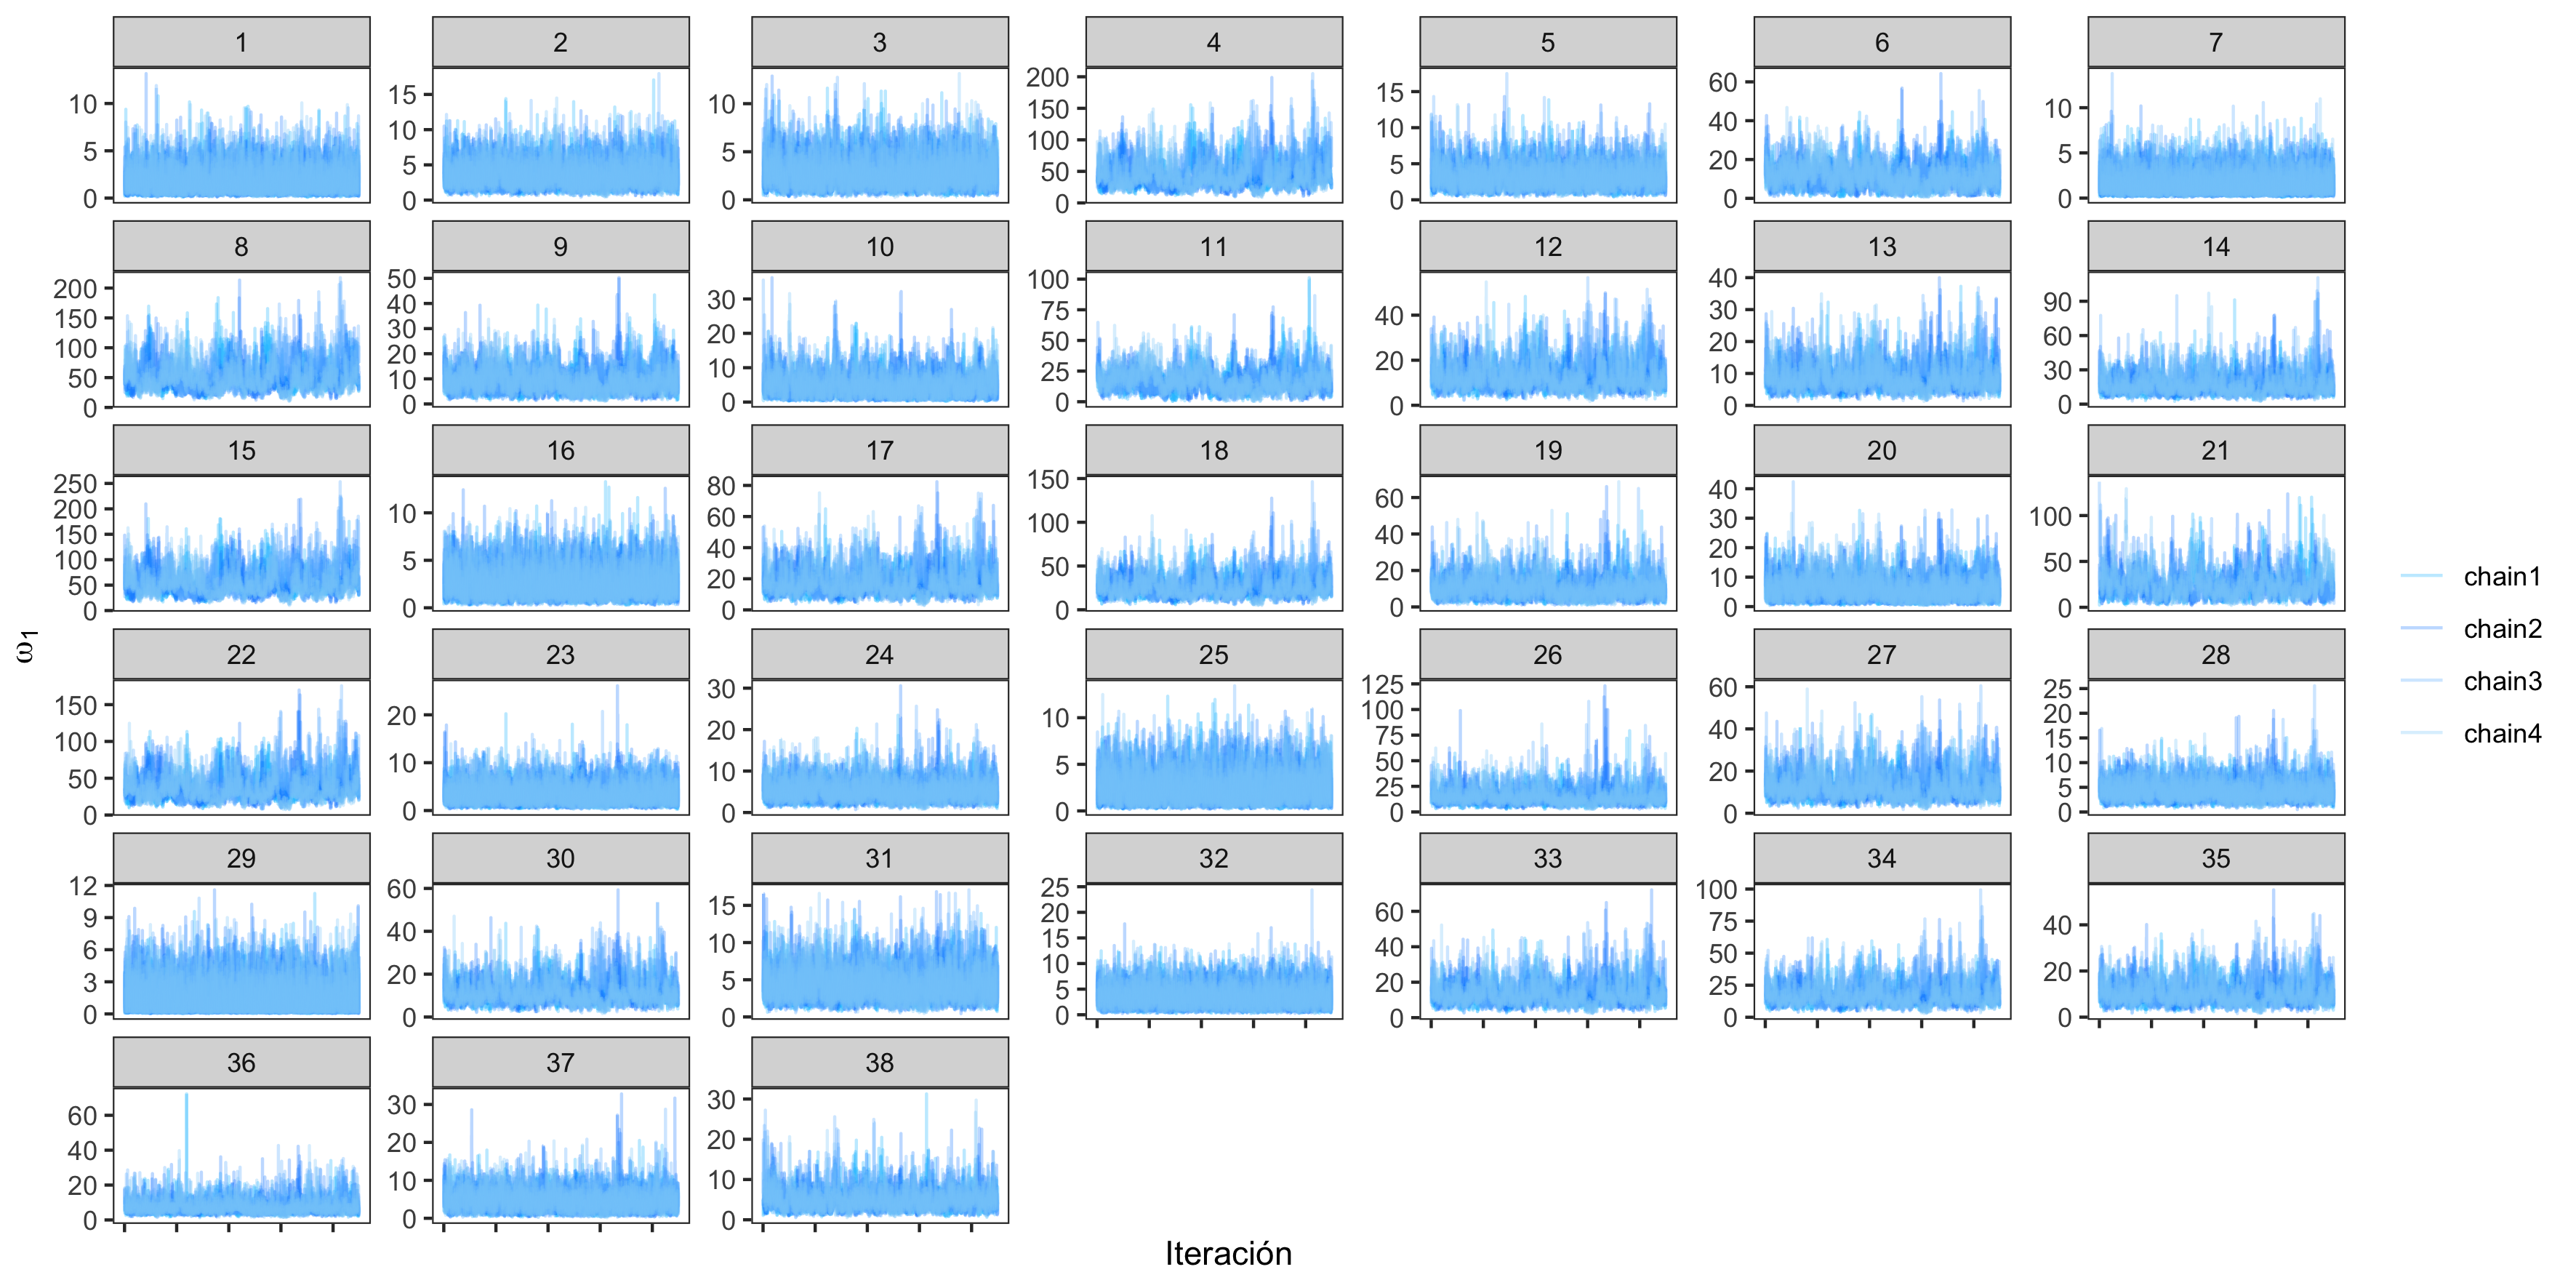
\includegraphics[width=10cm]{traceplots_omega1.png}
\caption{Valores simulados de $\omega_1$.}
\label{fig:traceplot_omega1}
\end{figure}

\begin{figure}[!htb]
\centering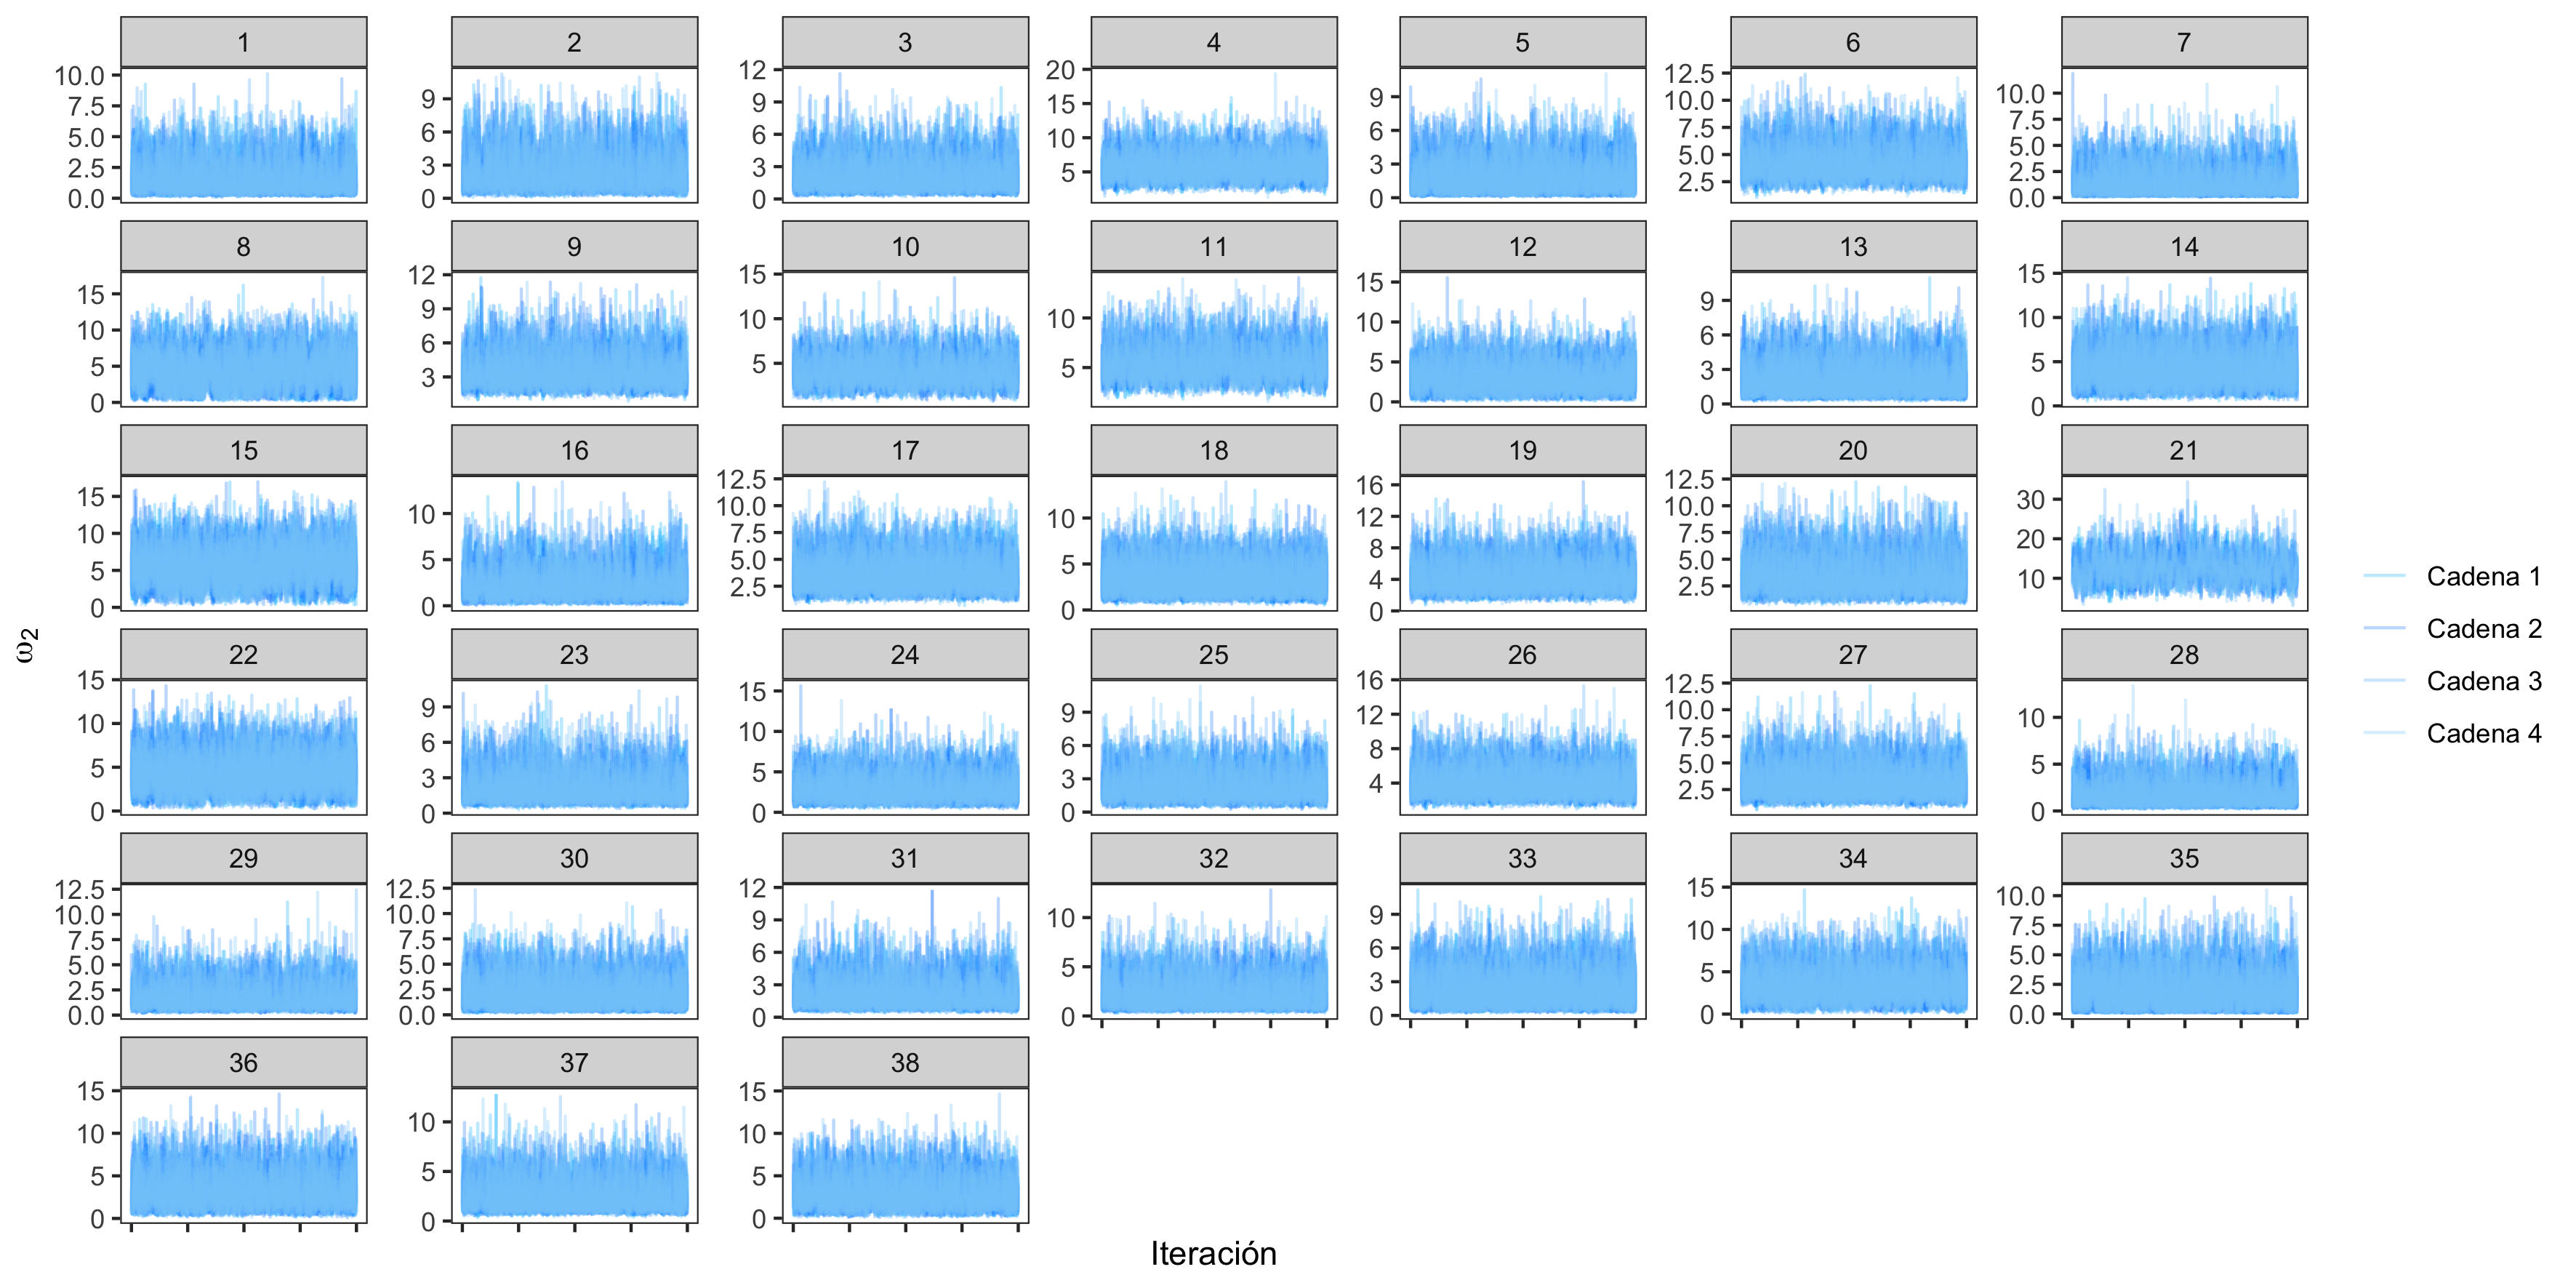
\includegraphics[width=10cm]{traceplots_omega2.png}
\caption{Valores simulados de $\omega_2$.}
\label{fig:traceplot_omega2}
\end{figure}

En las figuras \ref{fig:traceplot_omega1} y \ref{fig:traceplot_omega2} se encuentran las trazas de las cadenas para cada componente de los vectores $\omega_1$ y $\omega_2$. Como se mencionó en la sección \ref{sec:mh}, el hecho de que las cadenas se encimen sugiere que se alcanzó la convergencia a la distribución estacionaria y se pierde la dependencia de los valores iniciales. Por otro lado, en las figuras \ref{fig:ergodic_means_omega1} y \ref{fig:ergodic_means_omega2} se ve que la estimación del valor esperado converge para las distintas cadenas, indicando un comportamiento deseable de las simulaciones.

\begin{figure}[!htb]
\centering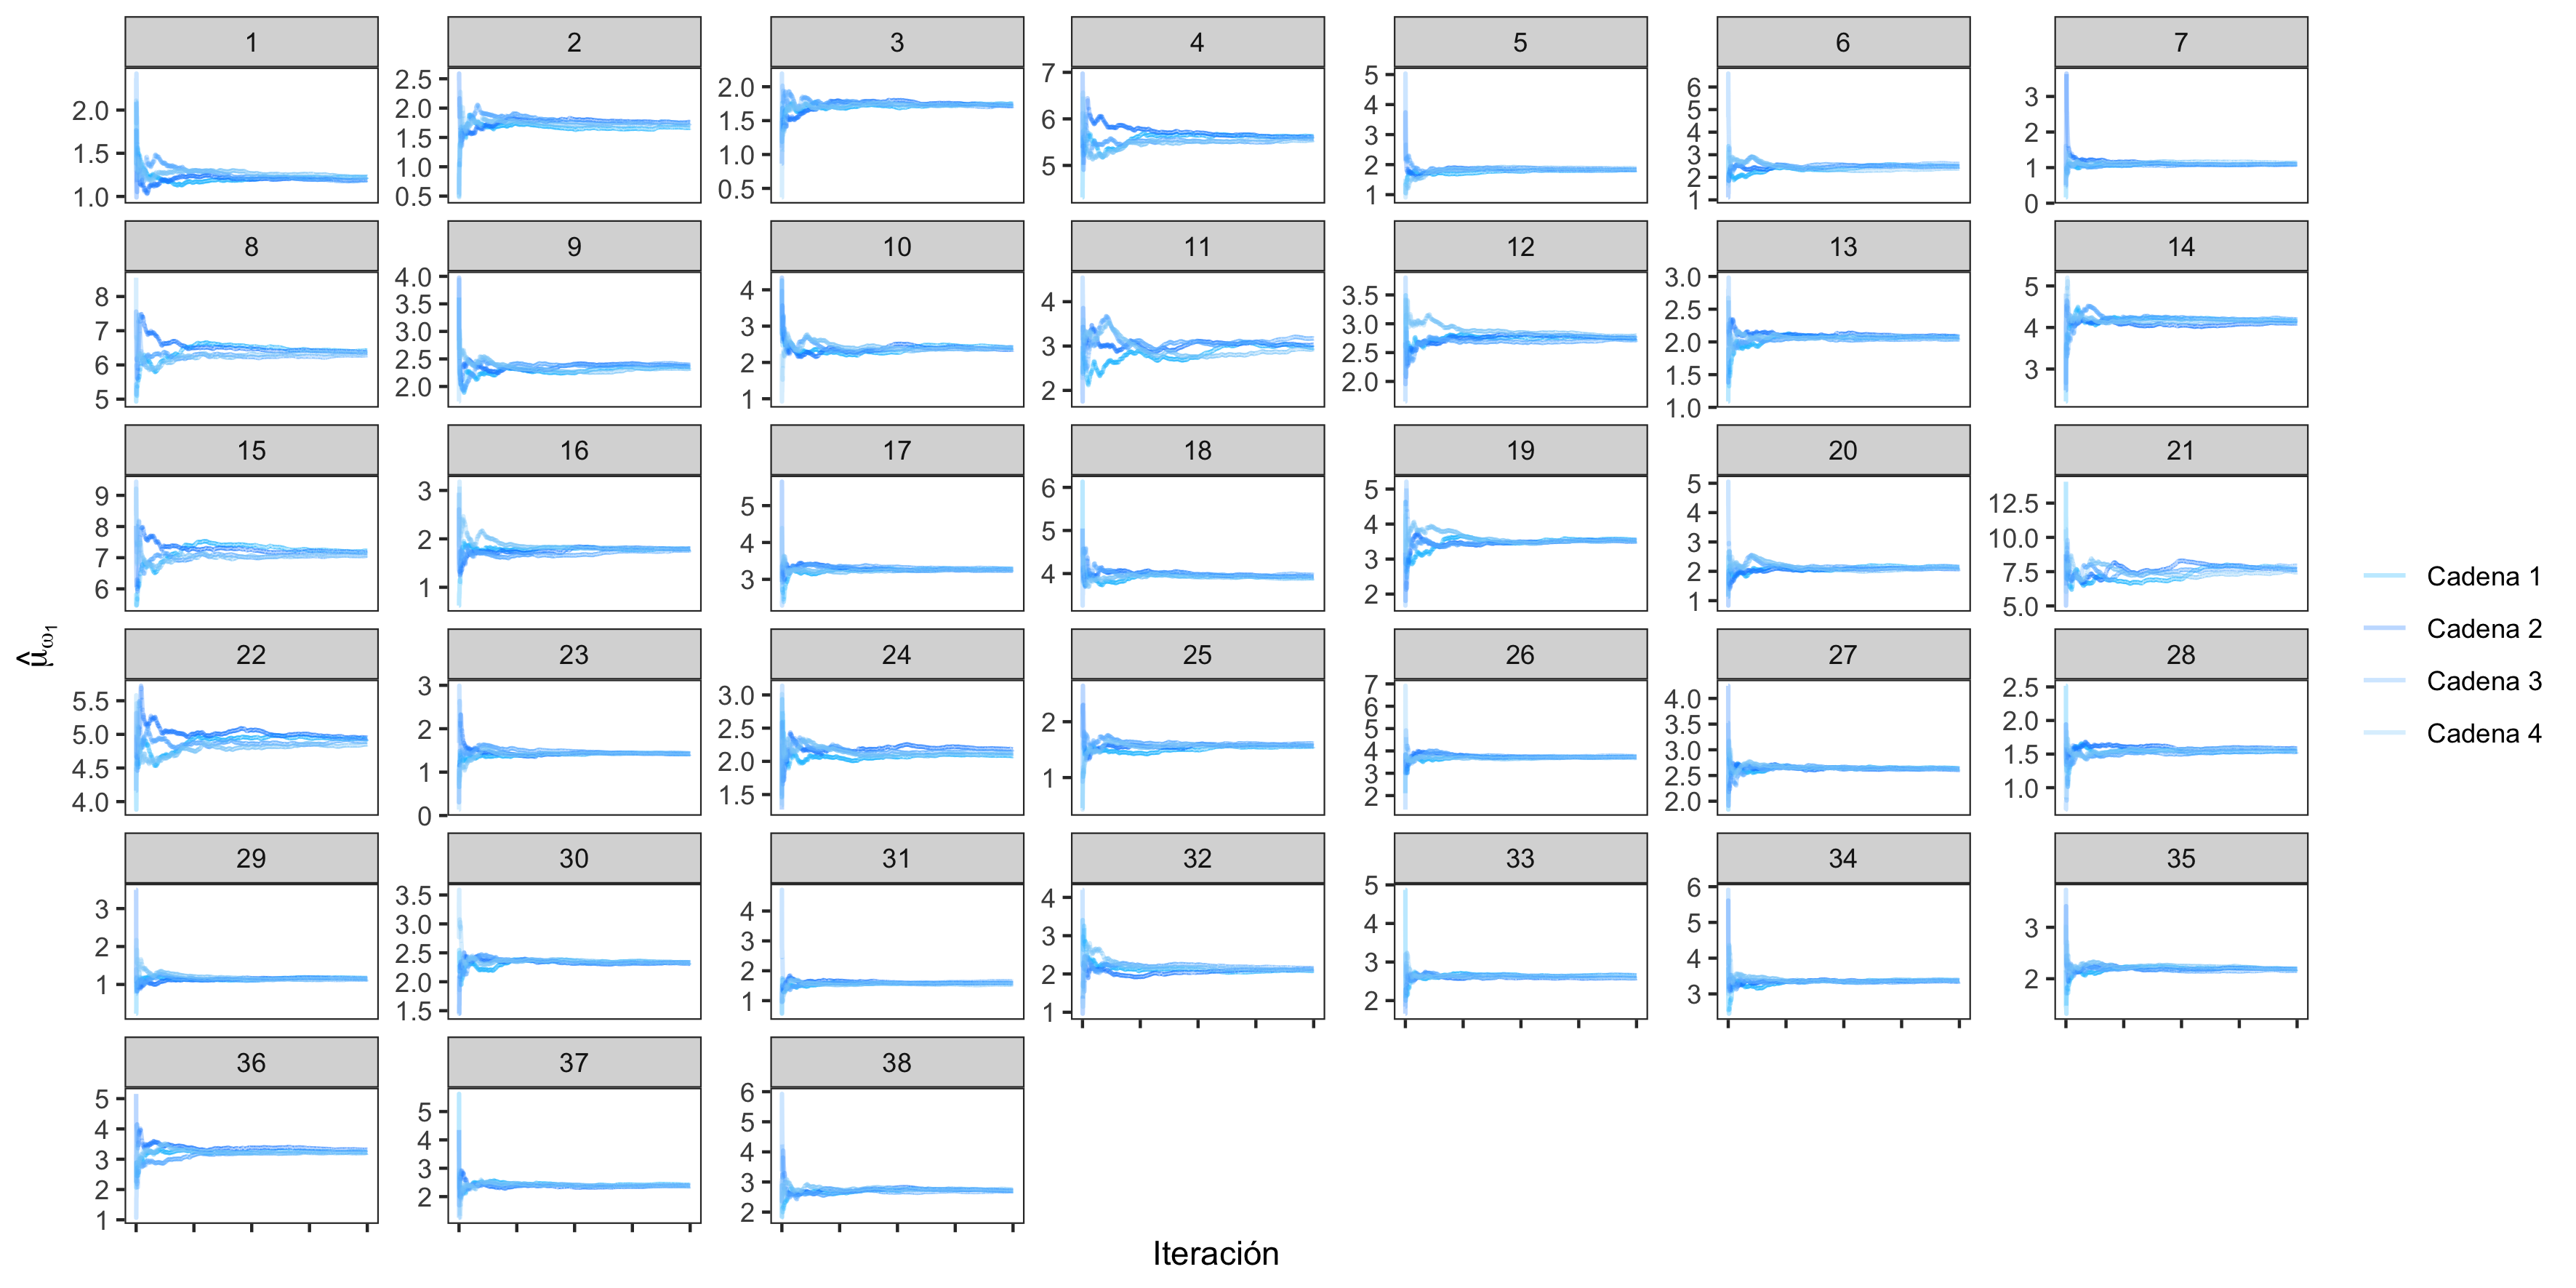
\includegraphics[width=10cm]{ergodic_means_omega1.png}
\caption{Gráfica de $E\left[ \omega_1 | datos \right]$ a través de las iteraciones.}
\label{fig:ergodic_means_omega1}
\end{figure}

\begin{figure}[!htb]
\centering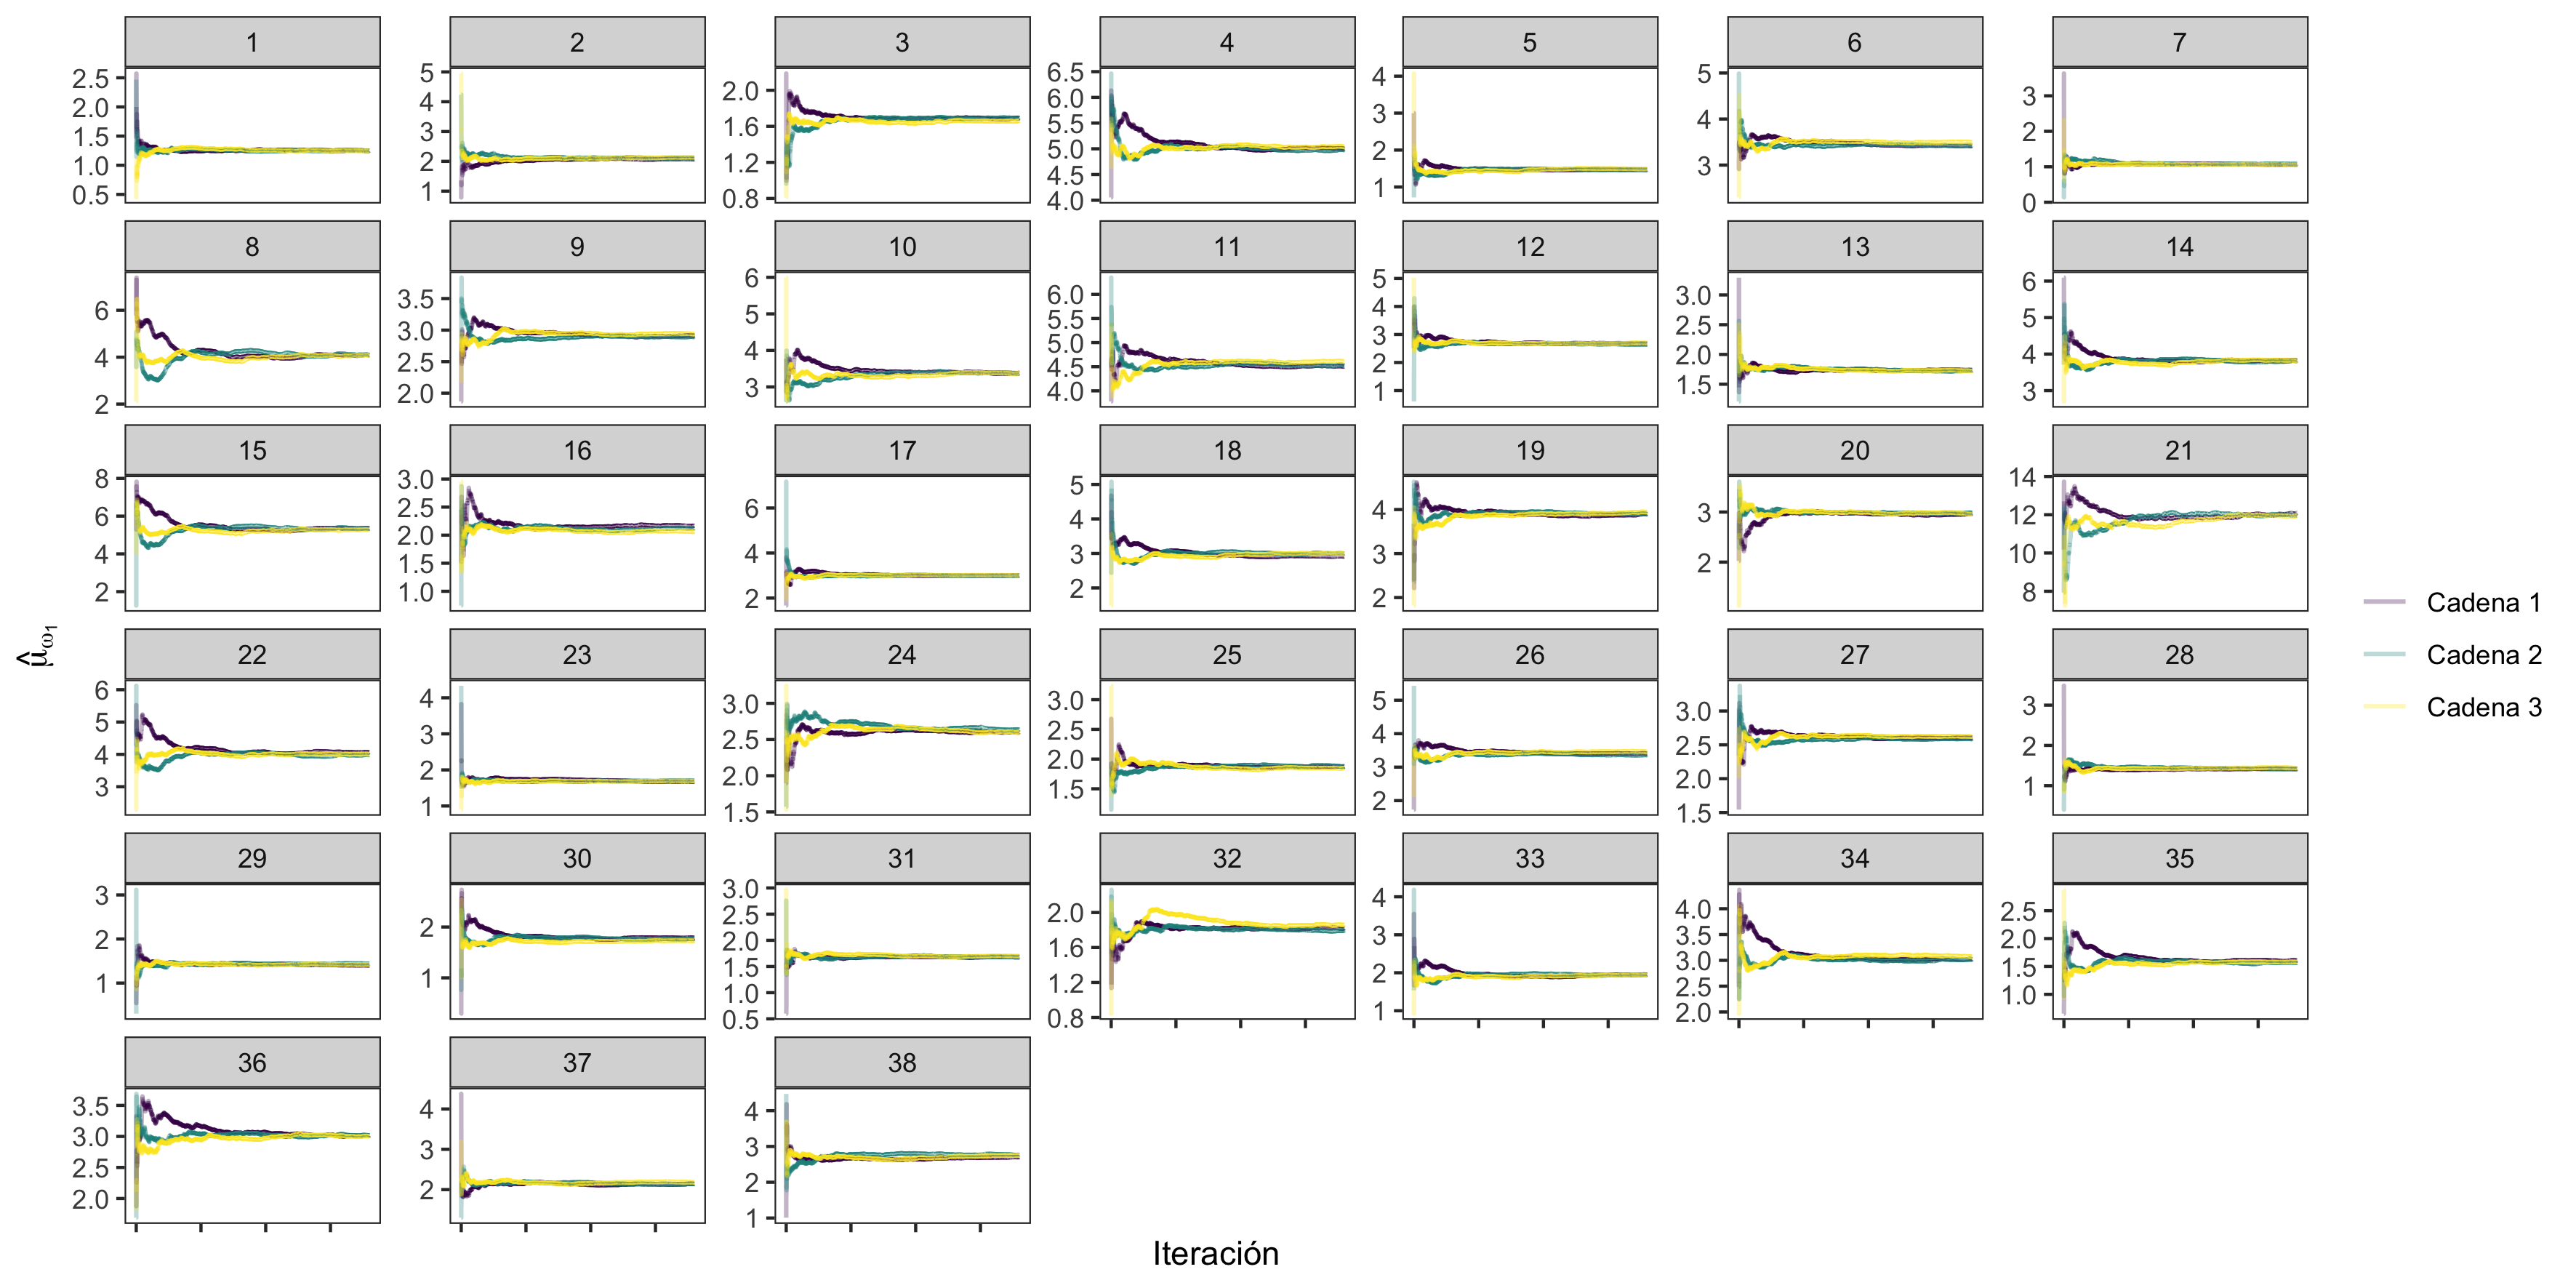
\includegraphics[width=10cm]{ergodic_means_omega2.png}
\caption{Gráfica de $E\left[ \omega_2 | datos\right]$ a través de las iteraciones.}
\label{fig:ergodic_means_omega2}
\end{figure}

\begin{figure}[!htb]
\centering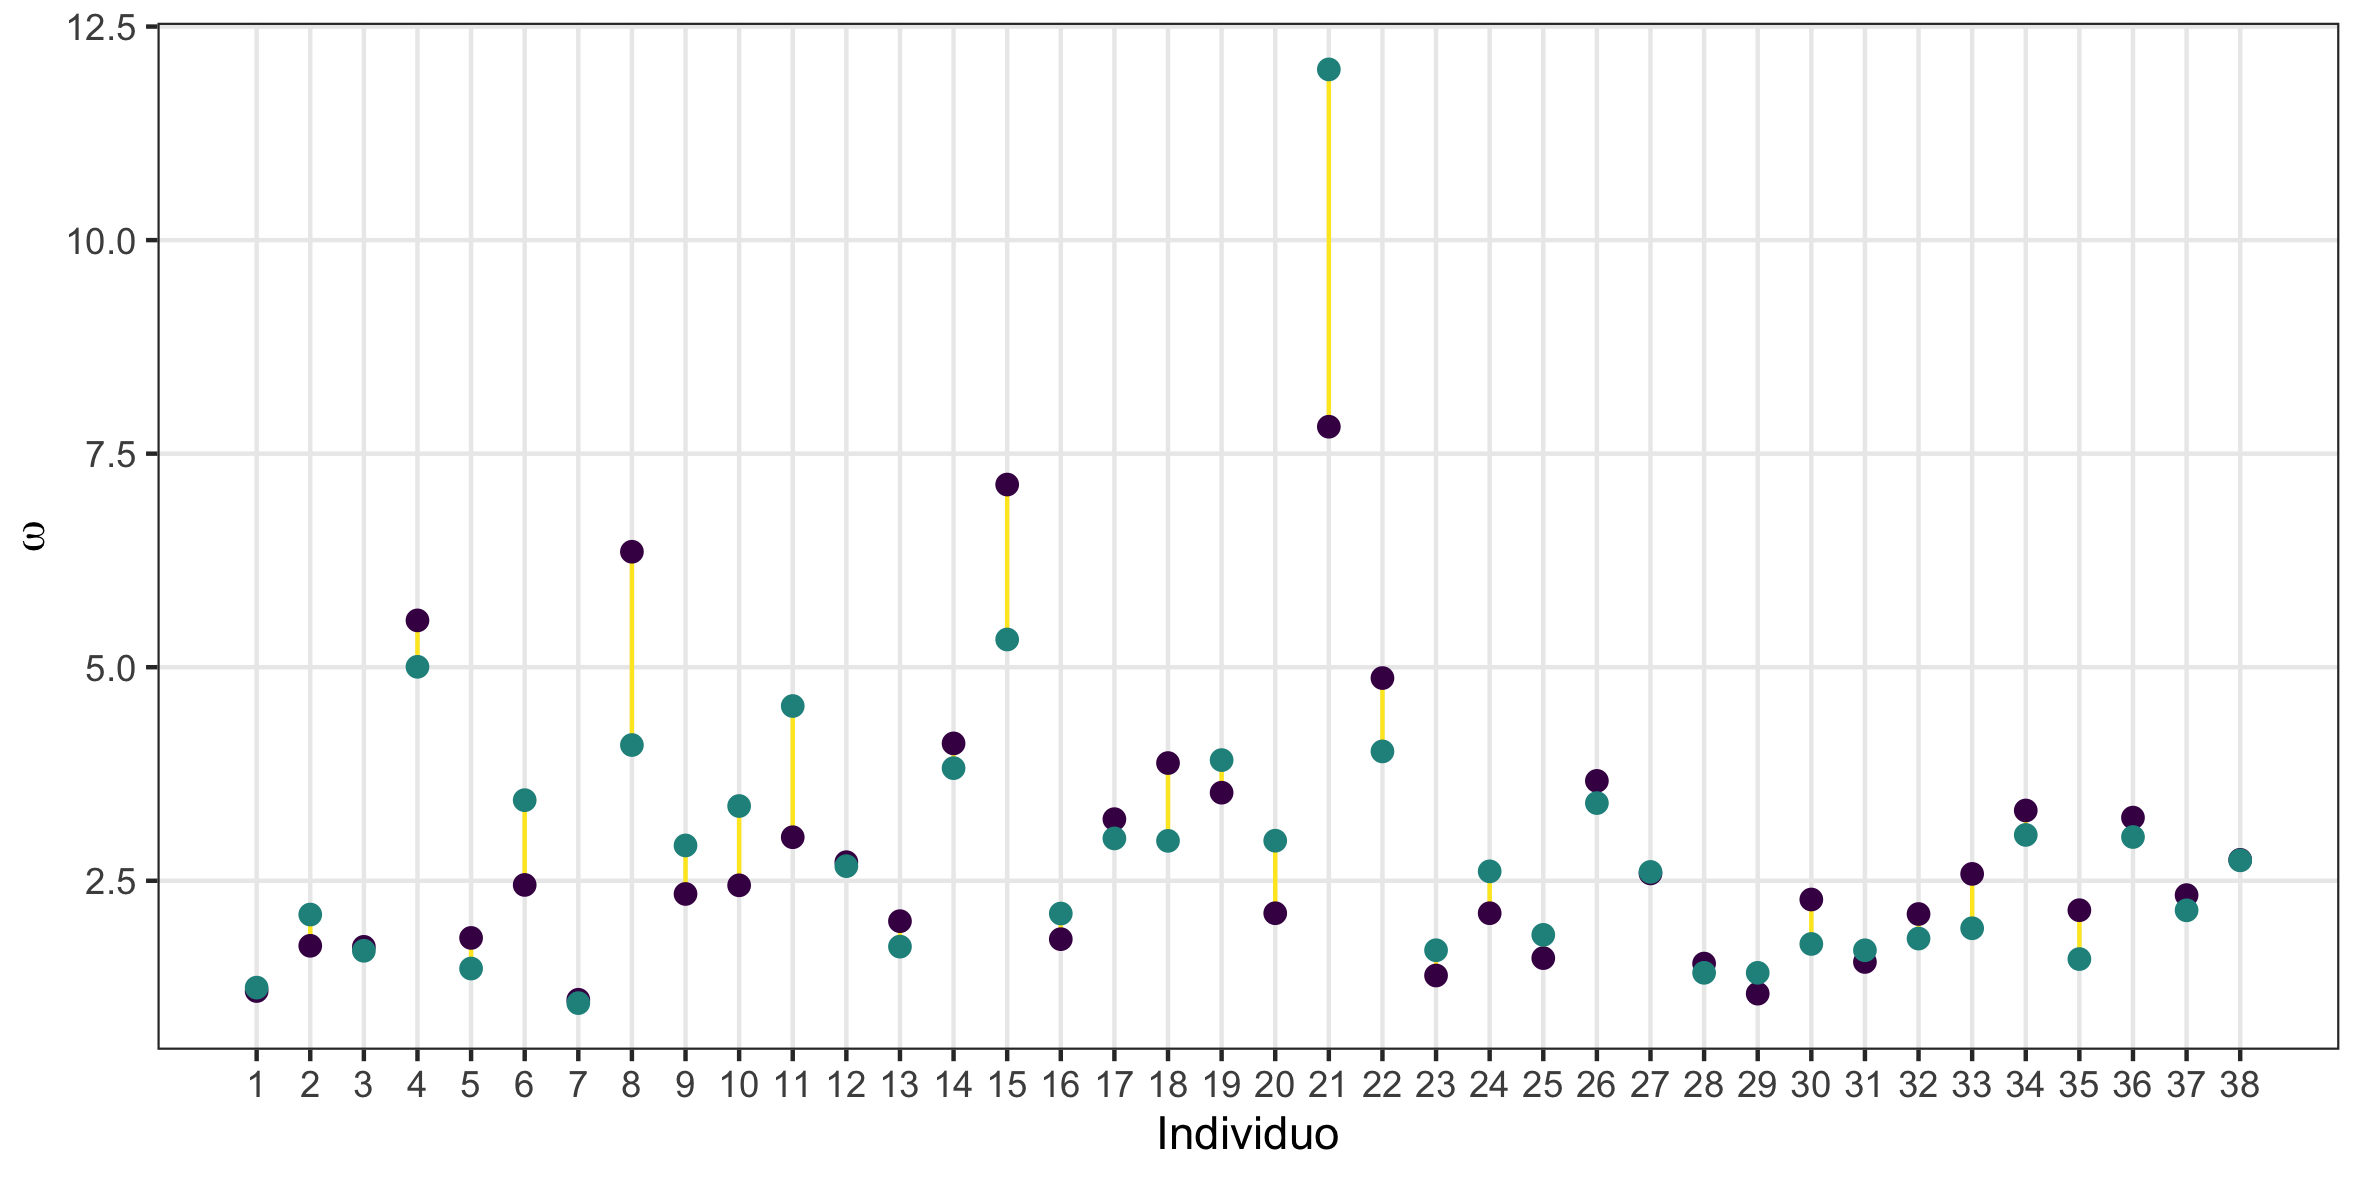
\includegraphics[width=10cm]{frailties.png}
\caption{Valores esperados de $\omega_1$ (morado) y $\omega_2$ (azul) por individuo.}
\label{fig:frailties}
\end{figure}

En la figura \ref{fig:frailties} se presenta una gráfica con las estimaciones de la media de $\omega_1$ y $\omega_2$ para cada uno de los individuos en cada cadena, similar a la que presentan \citet{nieto}. Un mayor valor de $\omega_i$ está relacionado con una mayor supervivencia, sin contar el efecto de las variables explicativas. Resalta el individuo número 21, el cual tiene un valor de $\omega_2$ mucho mayor a los demás pacientes. Esto se debe a que el individuo 21 presentó el mayor registro en $t_2$ por un amplio margen.

\newpage

Las estimaciones de las tasas de riesgo base (correspondientes a los pacientes de sexo femenino) para cada una de las variables $T_1$ y $T_2$ se presentan en las figuras \ref{fig:haz_lambda1} y \ref{fig:haz_lambda2}. En la gráfica se incluyen también intervalos de probabilidad de 95 \%. Se puede apreciar el suavizamiento de las estimaciones que se obtiene por utilizar la distribución inicial no paramétrica. Mientras más chicos se hacen los intervalos de la partición del tiempo, más suaves se verán estas funciones. Es interesante notar que, al introducir correlación entre las tasas $\lambda_j$, se tienen estimaciones de la tasa de riesgo distintas de cero aún en los intervalos de tiempo en donde no se presentan eventos de fallo \citep{nieto}. Gráficamente se pueden observar los crecimientos en la tasa de riesgo $\lambda_1$ (figura \ref{fig:haz_lambda1}) alrededor de los tiempos $t = 20$ y $t = 150$, al igual que los crecimientos en la tasa de riesgo $\lambda_2$ (figura \ref{fig:haz_lambda2}) alrededor de los tiempos $t = 20$ y $t = 200$. Se puede apreciar también que la tasa de riesgo $\lambda_1$ es mayor a $\lambda_2$ en la mayor parte del tiempo estudiado.

\begin{figure}[!htb]
\centering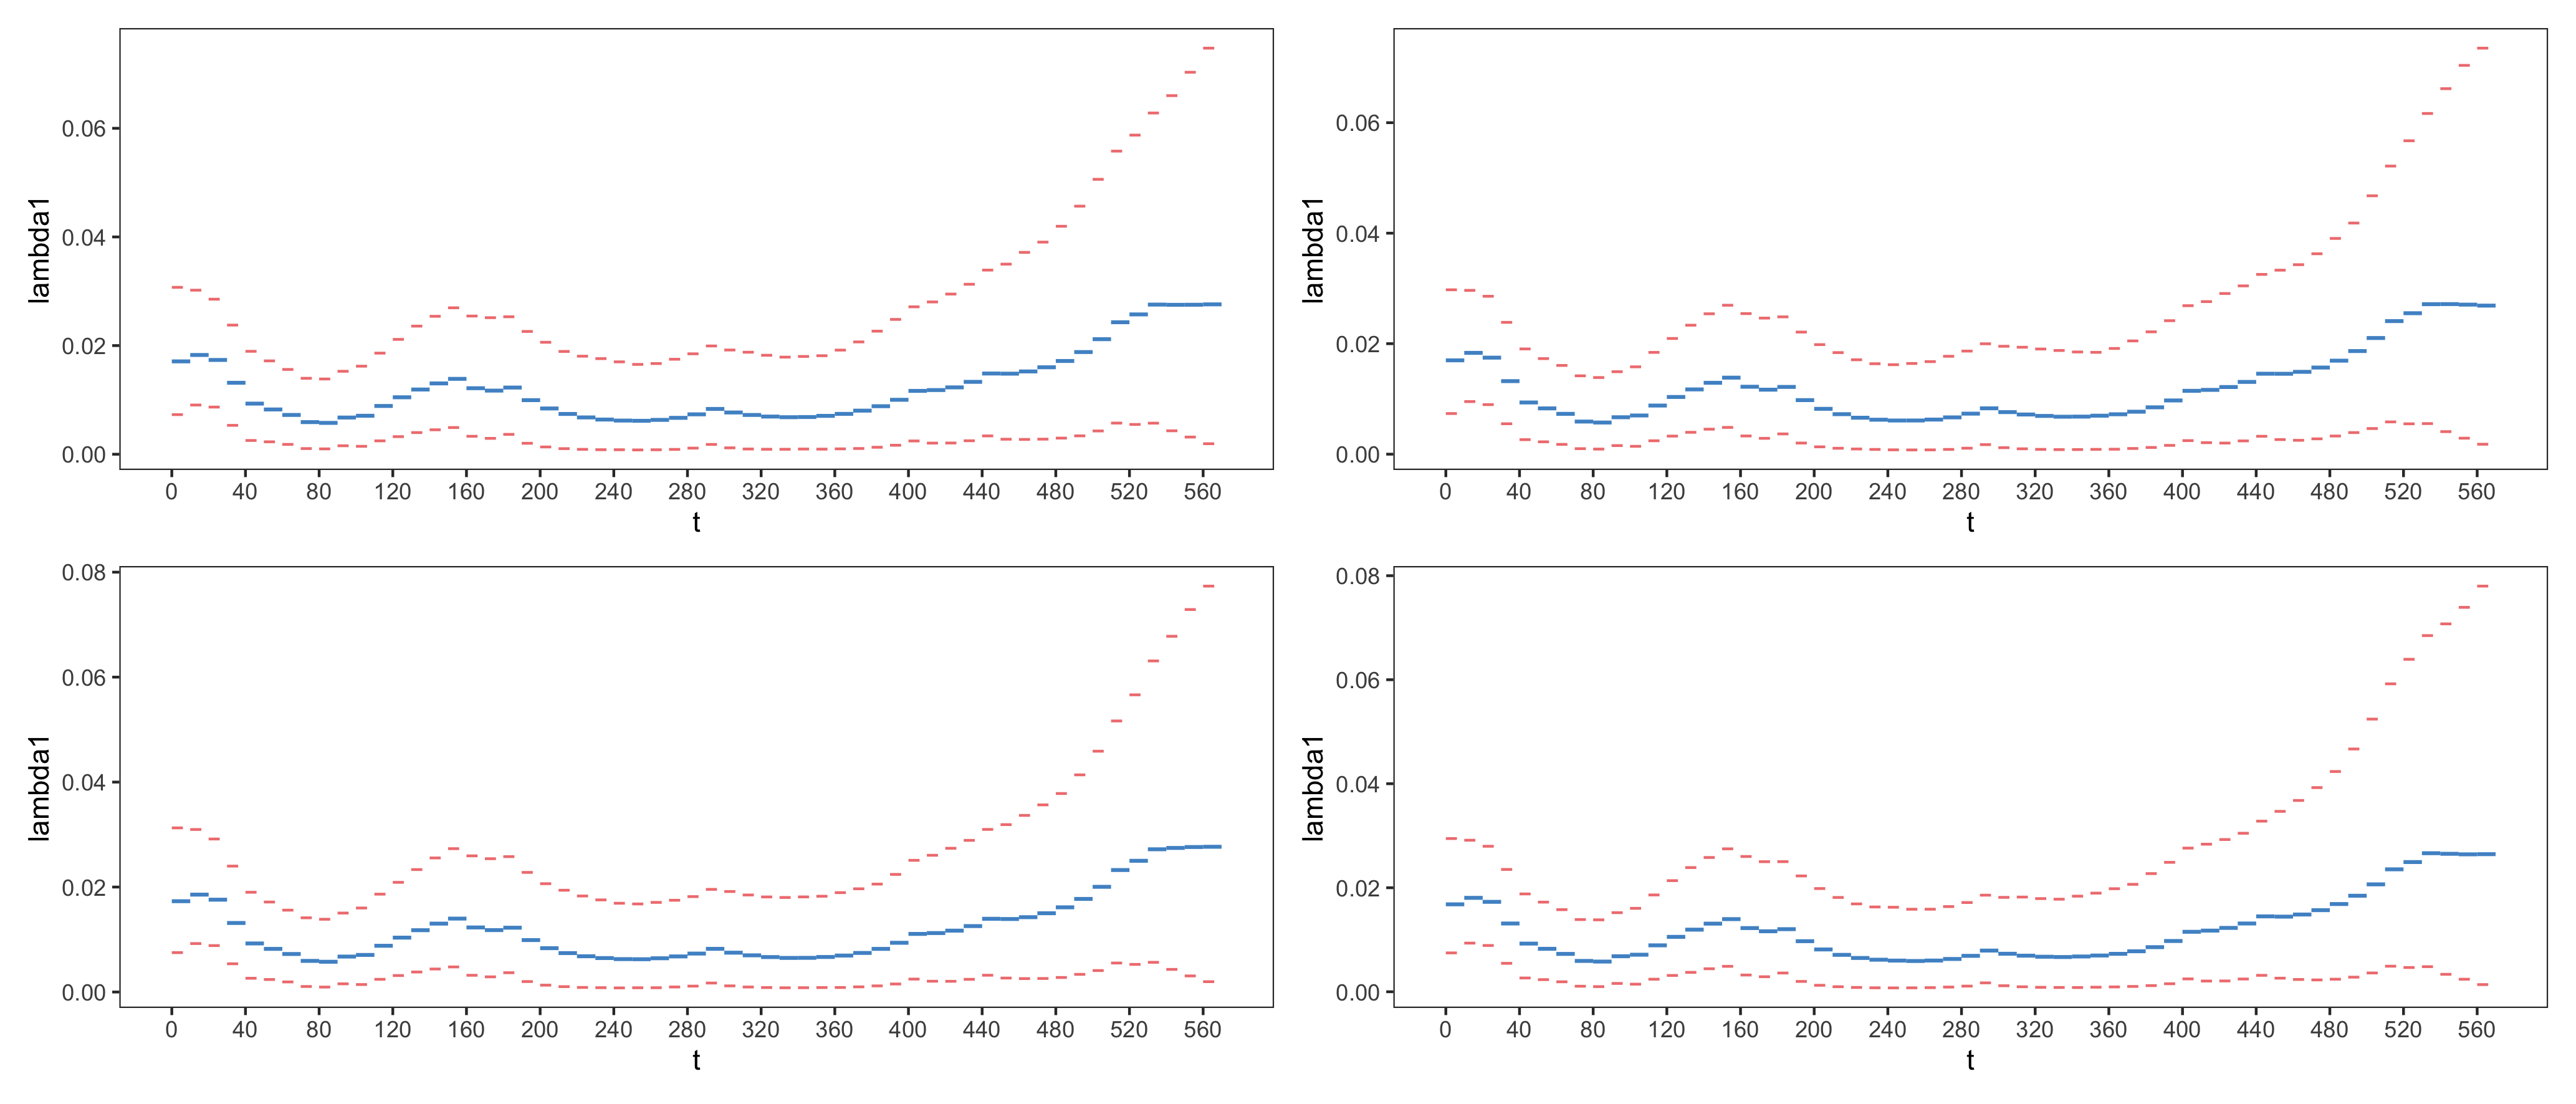
\includegraphics[width=10cm]{hazard1.png}
\caption{Valores esperados de la tasa de riesgo $\lambda_1$.}
\label{fig:haz_lambda1}
\end{figure}

\begin{figure}[!htb]
\centering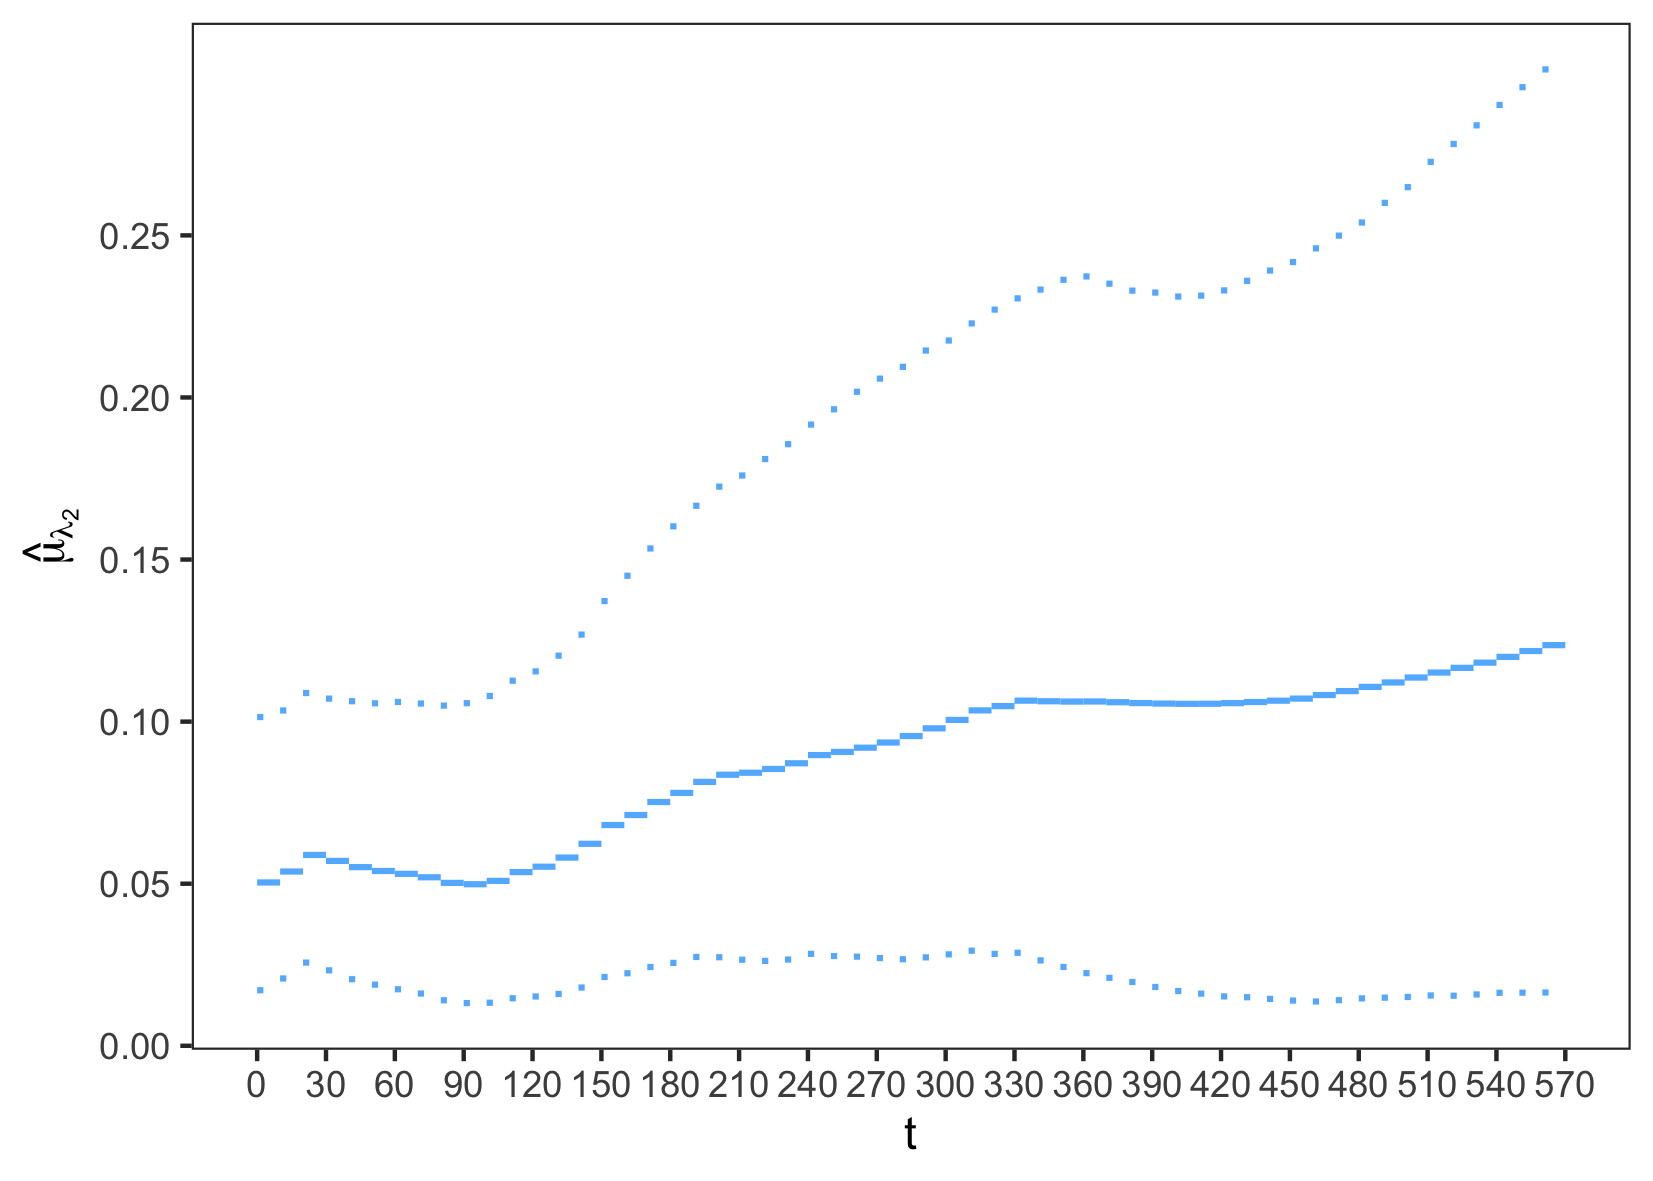
\includegraphics[width=10cm]{hazard2.png}
\caption{Valores esperados de la tasa de riesgo $\lambda_2$.}
\label{fig:haz_lambda2}
\end{figure}

\newpage

En la figura \ref{fig:surv_fun_marginal} se pueden ver las funciones de supervivencia marginales para ambos tiempos de fallo. Es interesante notar que la función de supervivencia de $S(t_2)$ es mayor a $S(t_1)$ hasta alrededor de $t=250$, donde las funciones se intersectan. Este comportamiento es congruente con lo observado en las tasas de riesgo. En la figura \ref{fig:surv_fun} se muestra la función de supervivencia conjunta $S(t_1, t_2)$ junto con sus curvas de nivel. Esta función de supervivencia conjunta se obtiene al evaluar las funciones de supervivencia marginales en la cópula de supervivencia \eqref{copula_modelo}, esto es, $S(t_1, t_2) = \widehat{C}(S_1(t_1), S_2(t_2))$.

\begin{figure}[!htb]
\centering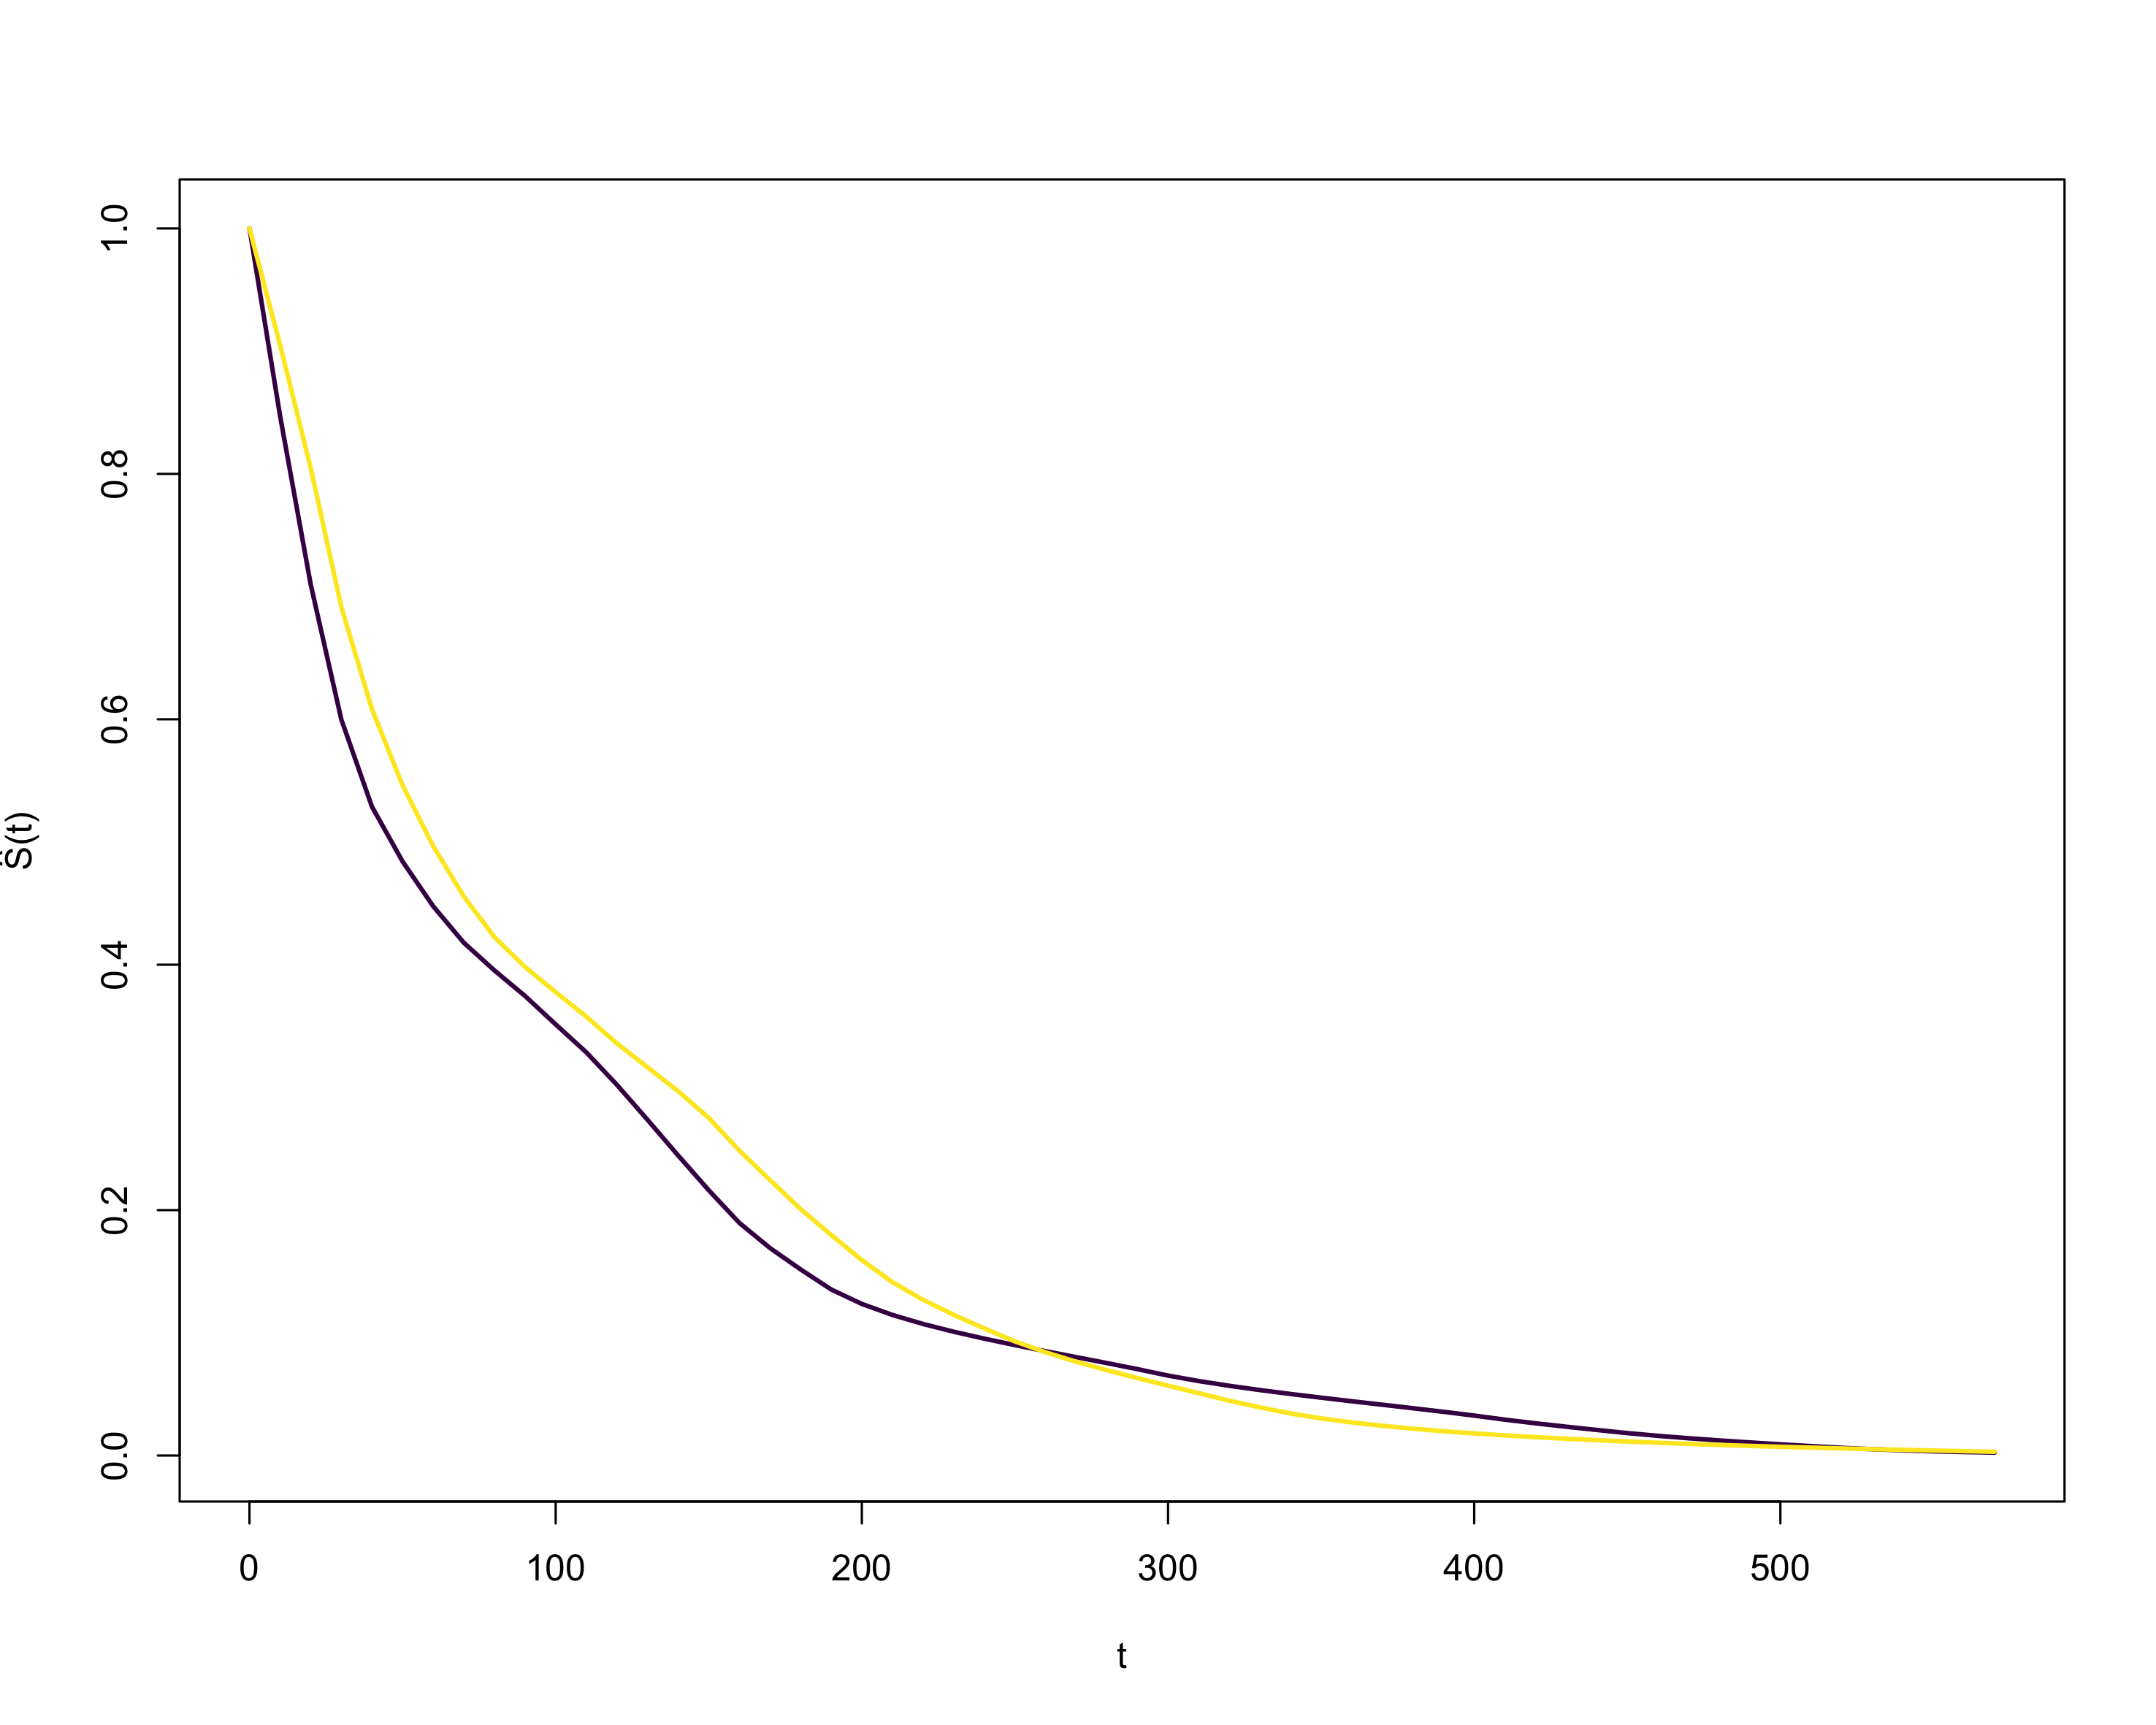
\includegraphics[width=10cm]{surv_fun_marginal.png}
\caption{Valores esperados de las funciones de supervivencia $S(t_1)$ (morado) y $S(t_2)$ (amarillo).}
\label{fig:surv_fun_marginal}
\end{figure}

\begin{figure}[!htb]
    \centering
    \begin{subfigure}[t]{0.45\textwidth}
        \centering
        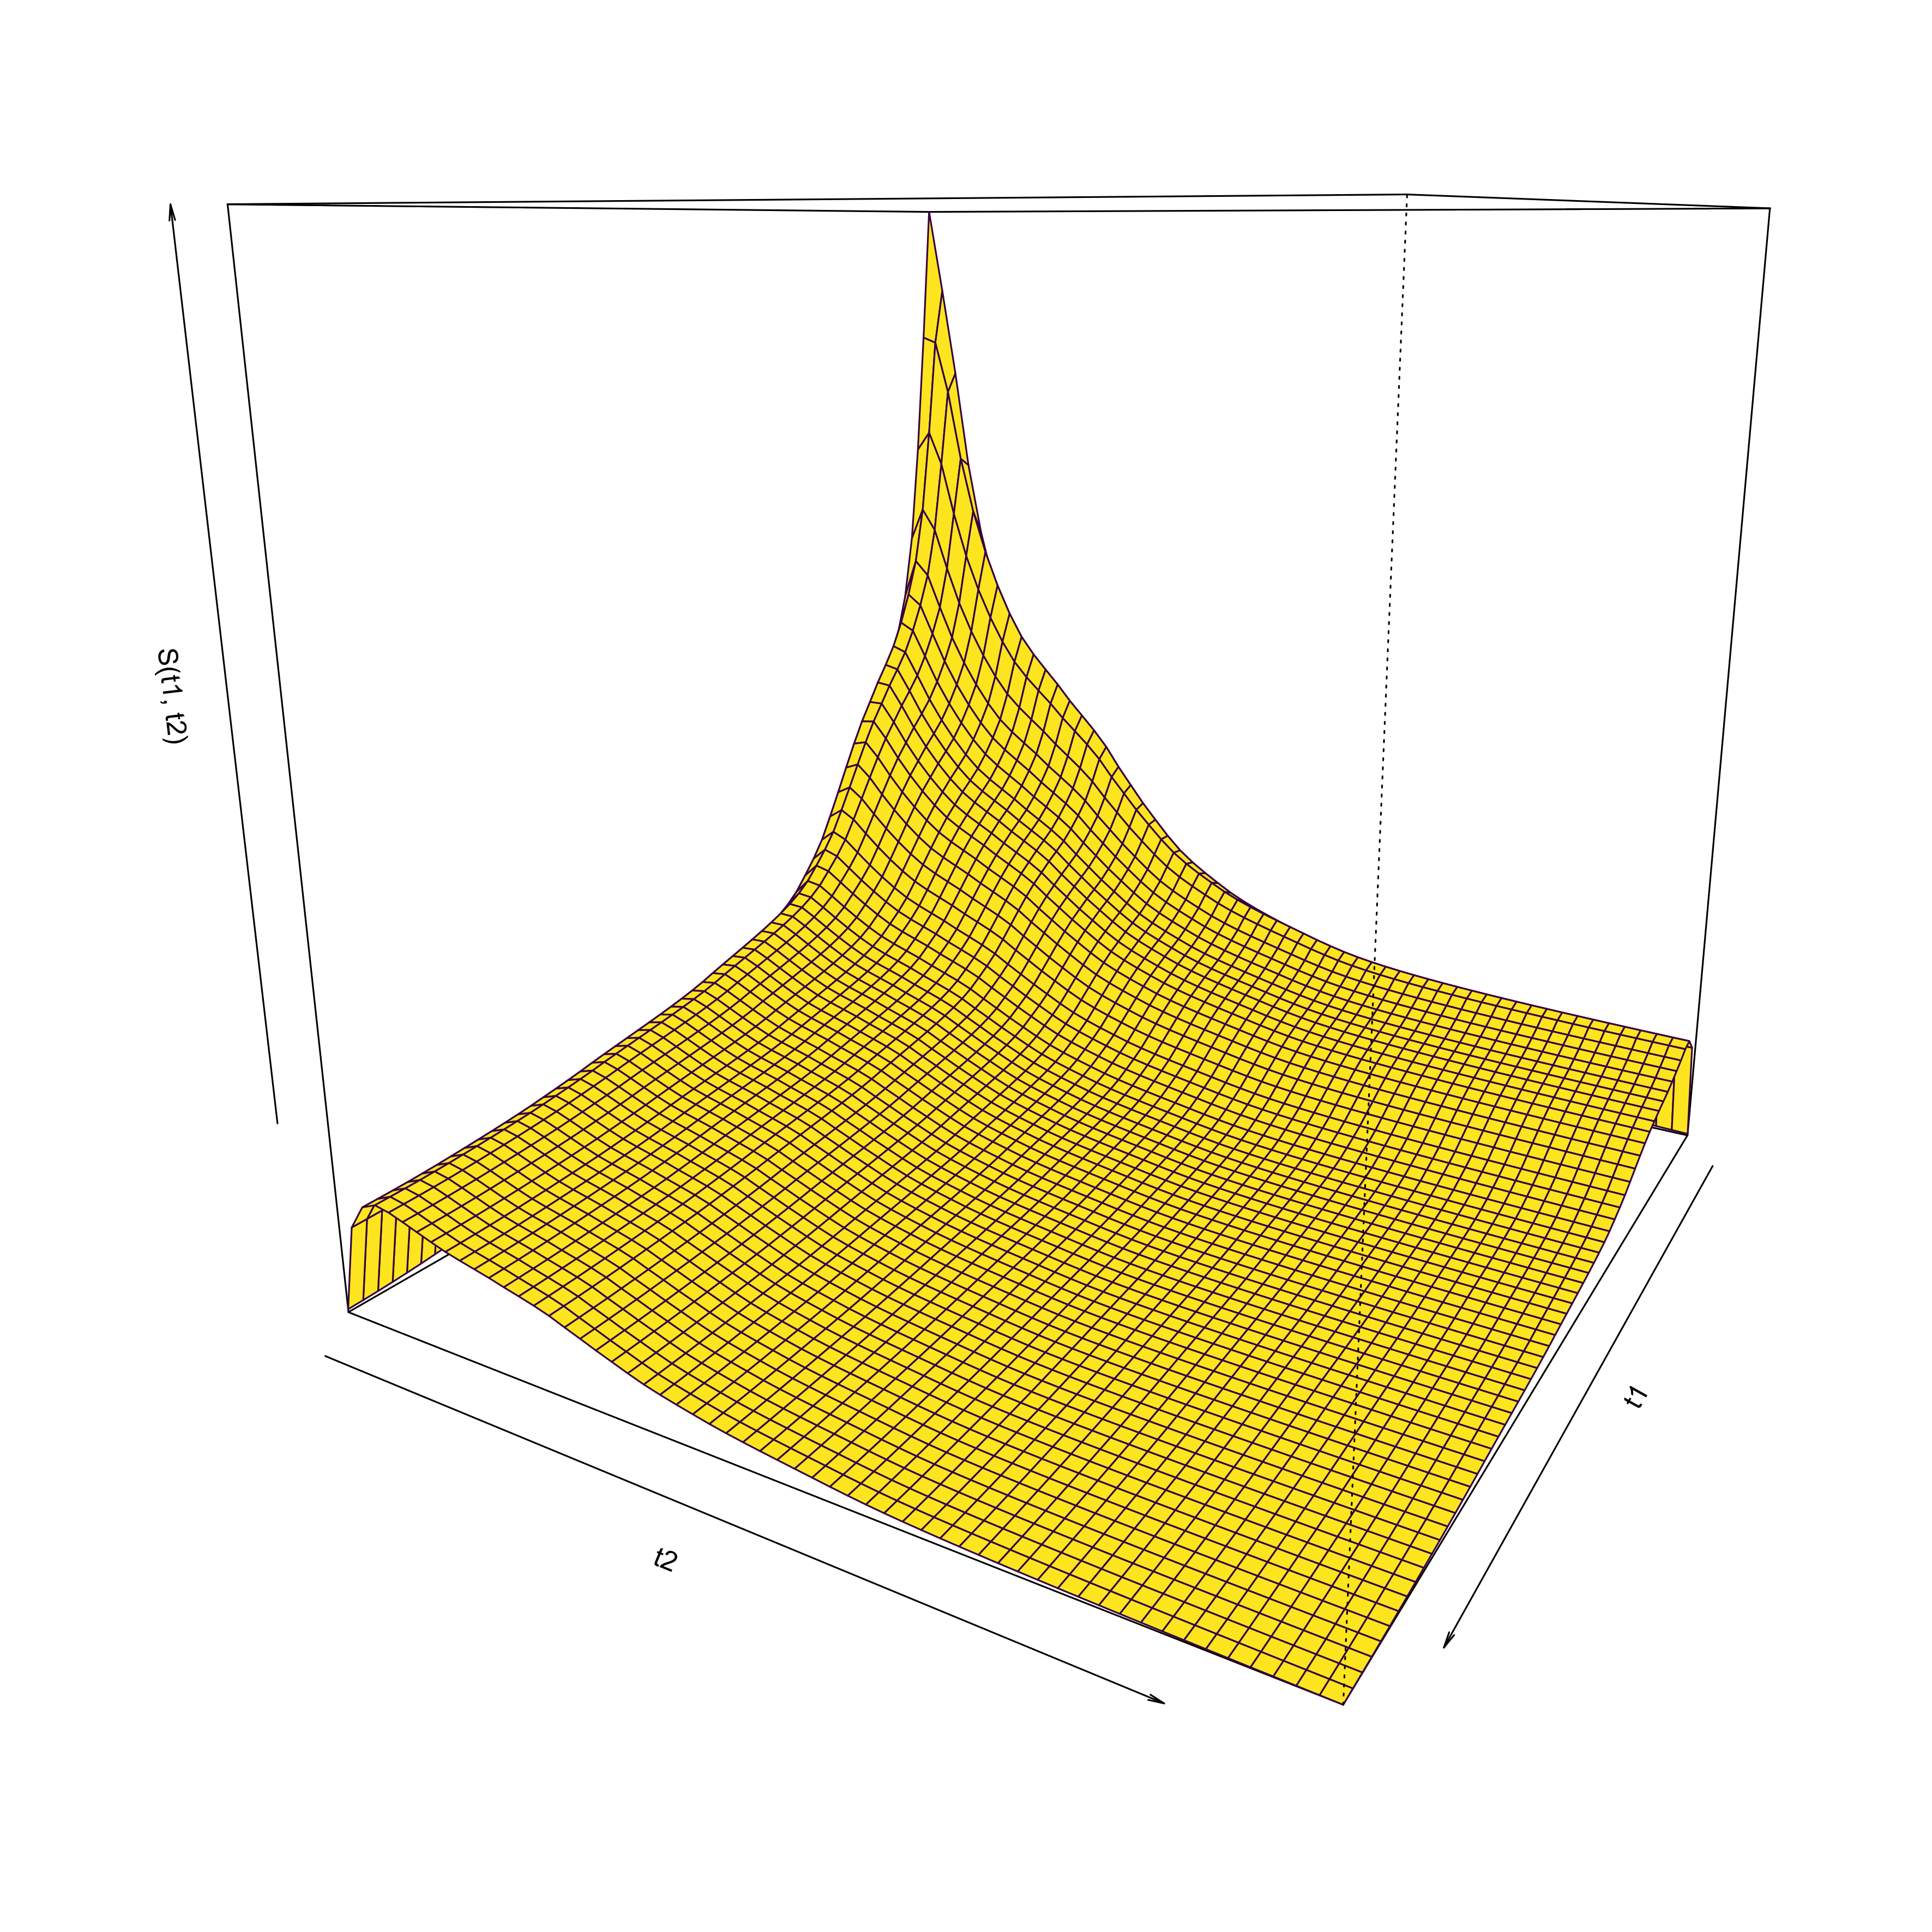
\includegraphics[width=\linewidth]{surv_fun.png}
        \caption{Estimación $S(t_1, t_2)$.}
        \label{fig:surv_fun_3d}
    \end{subfigure}
    \hfill
    \begin{subfigure}[t]{0.45\textwidth}
        \centering
        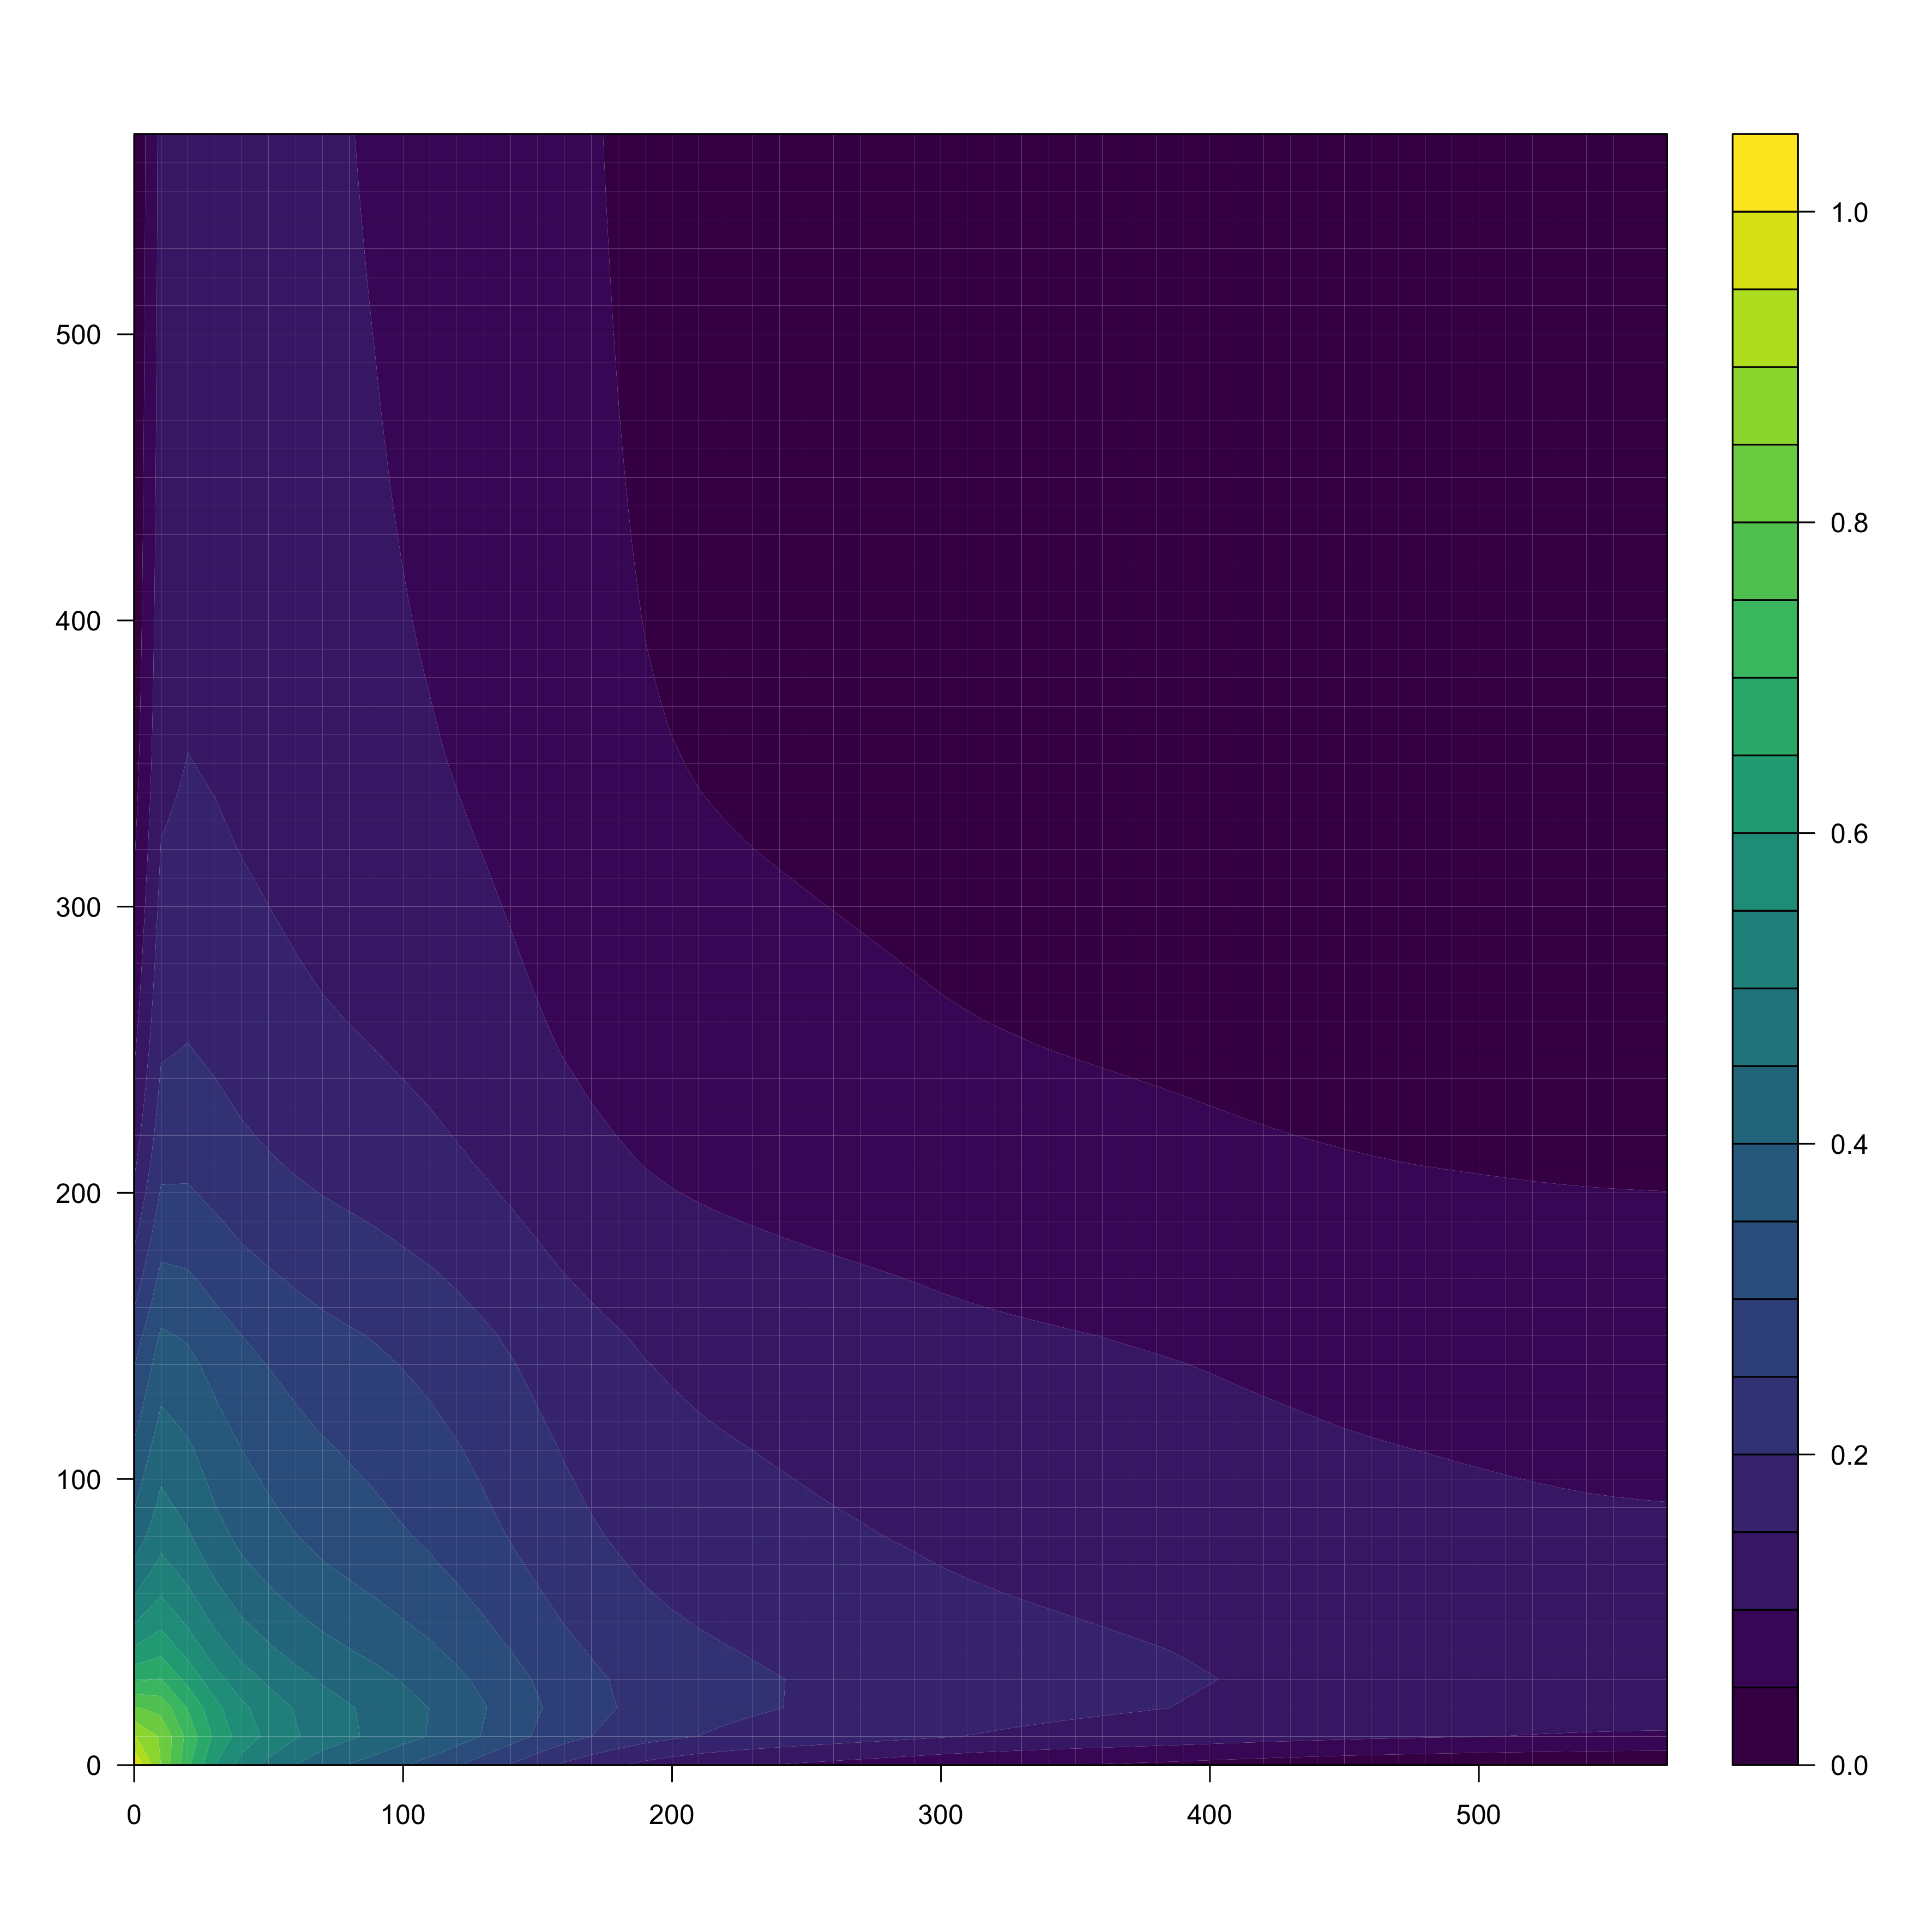
\includegraphics[width=\linewidth]{surv_fun_contour.png} 
        \caption{Curvas de nivel de $S(t_1, t_2)$.}
        \label{fig:surv_fun_contour}
    \end{subfigure}
    \caption{Gráfica y curvas de nivel de la función de supervivencia conjunta $S(t_1, t_2)$.}
    \label{fig:surv_fun}
\end{figure}

\clearpage

Se incluyen también los diagnósticos para el parámetro $\gamma$ que modela la correlación entre los tiempos de fallo en la figura \ref{fig:gamma}. La traza de la cadena en el panel \ref{fig:gamma_trace} sugiere que la distribución posterior es explorada de manera satisfactoria y la convergencia de las estimaciones de la media no señala ningún comportamiento indeseable (figura \ref{fig:gamma_means}). Se presenta un suavizamiento del histograma utilizando las simulaciones de las tres cadenas con la función \texttt{geom\_density} del paquete \texttt{ggplot2} \citep{ggplot} en el panel \ref{fig:gamma_densities}. La estimación posterior de $E \left[ \gamma | datos \right]$ usando las simulaciones de las tres cadenas es de 2.46. El intervalo de probabilidad de 0.95 para $\gamma$ obtenido con los cuantiles 0.025 y 0.975 es $(0.21, 10.14)$.

\begin{figure}[!htb]
    \centering
    \begin{subfigure}[t]{0.45\textwidth}
       \centering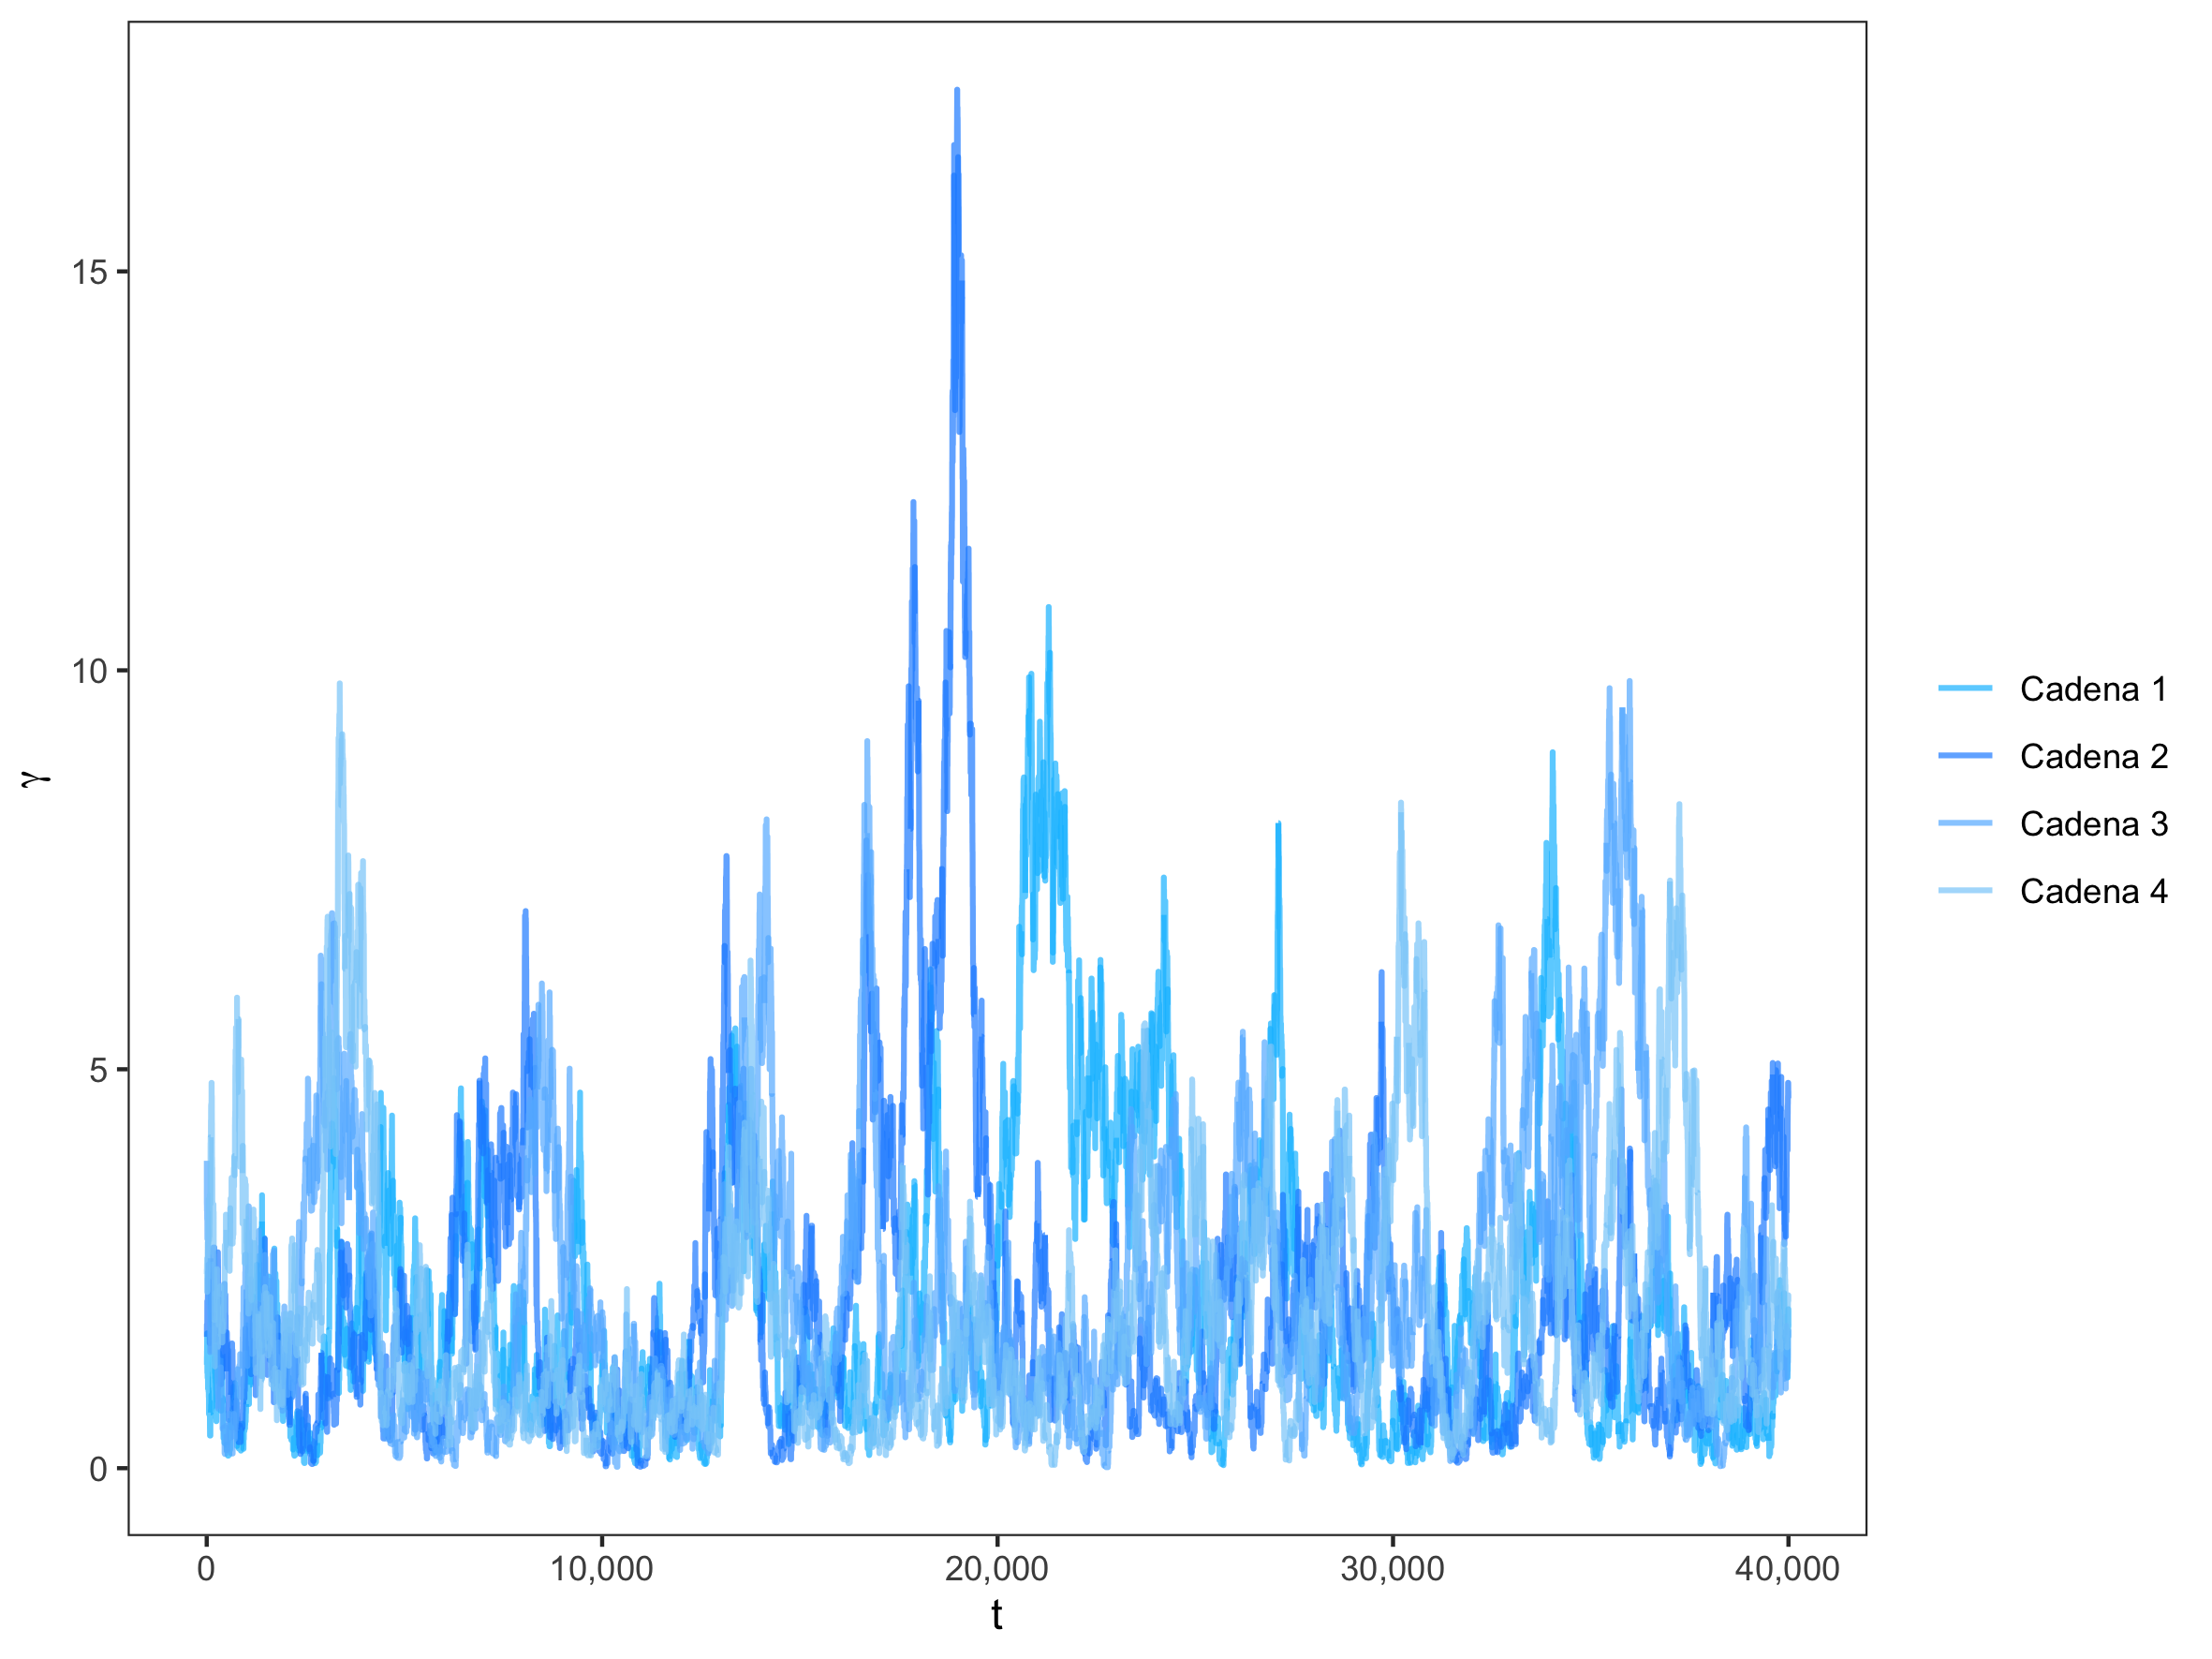
\includegraphics[width=\linewidth]{gamma_traceplot.png}
       \caption{Valores simulados de $\gamma$.}
       \label{fig:gamma_trace}
    \end{subfigure}
    \hfill
    \begin{subfigure}[t]{0.45\textwidth}
      \centering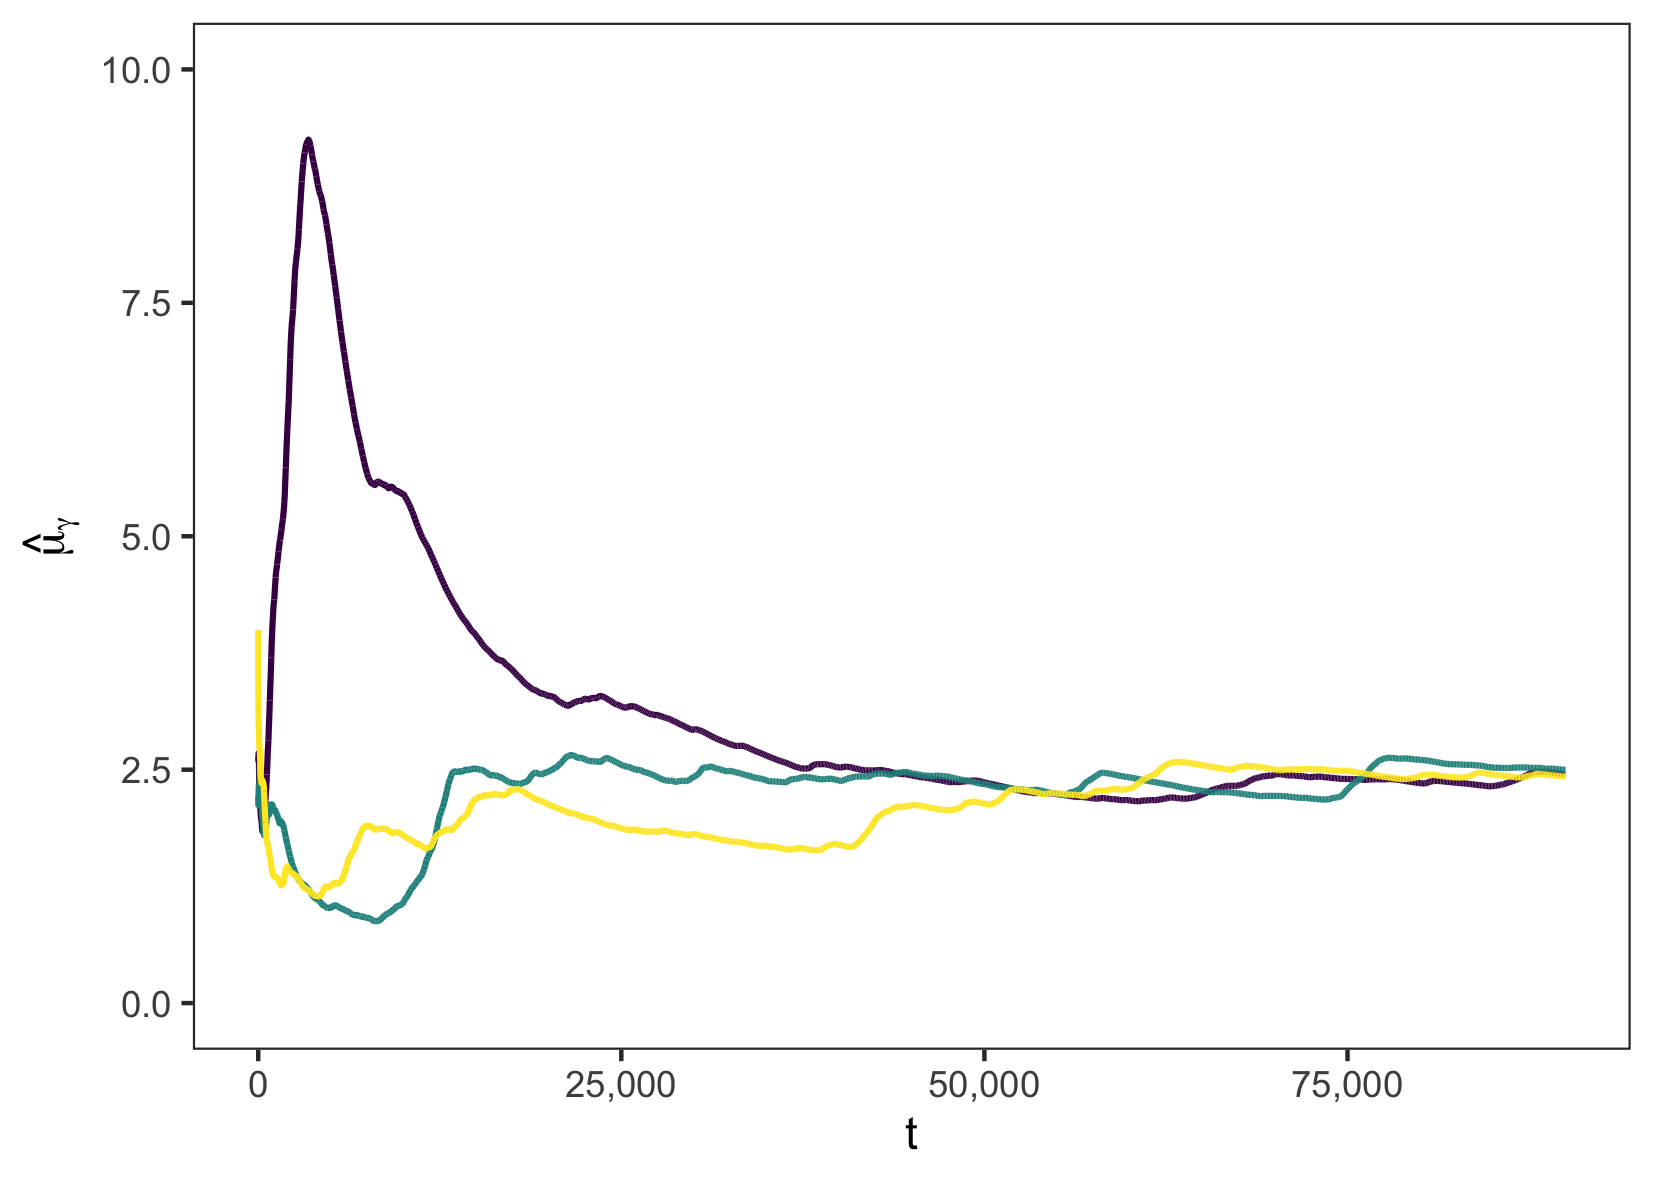
\includegraphics[width=\linewidth]{gamma_ergodic_means.png}
      \caption{Evolución de $E \left[ \gamma | datos \right]$ en cada iteración.}
      \label{fig:gamma_means}
    \end{subfigure}

    \vspace{0.2cm}
    \begin{subfigure}[t]{\textwidth}
    \centering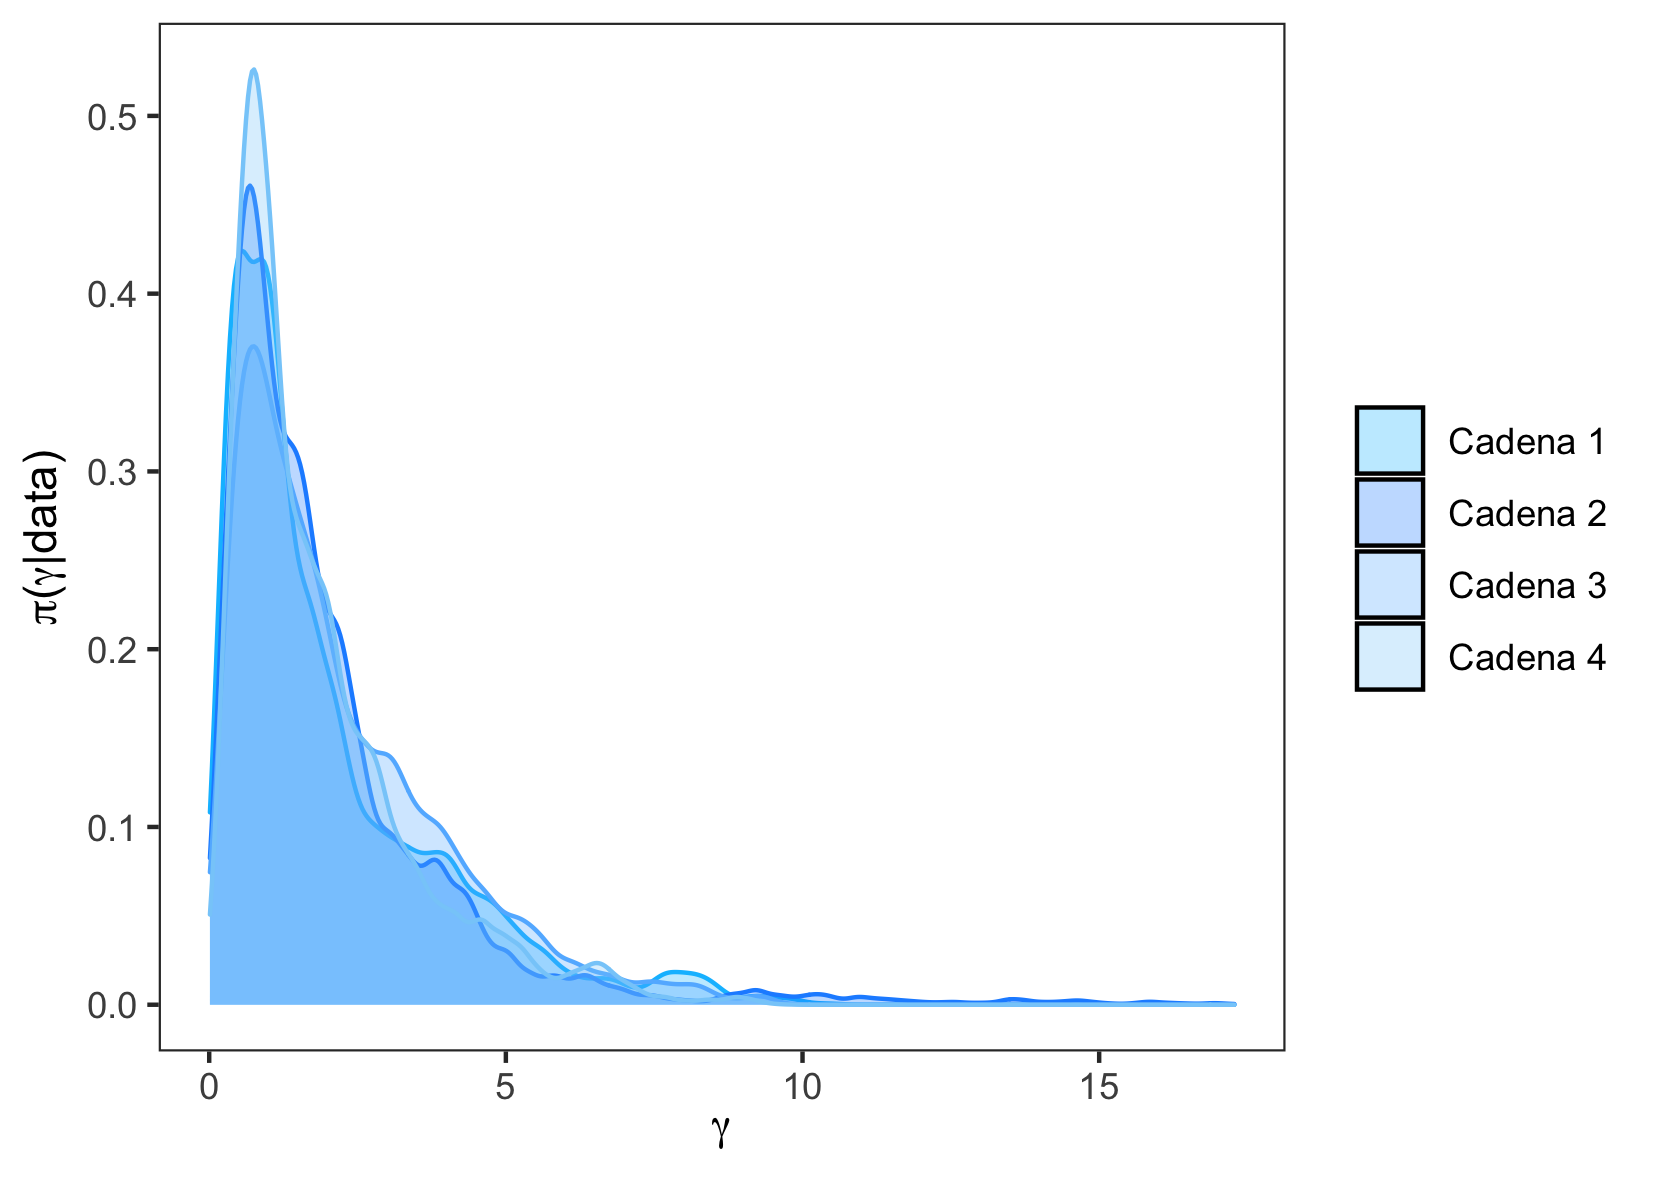
\includegraphics[width=\linewidth]{gamma_densities.png}
    \caption{Suavizamiento con kernel gaussiano para $\pi (\gamma | datos)$.}
    \label{fig:gamma_densities}
    \end{subfigure}
    \caption{Diagnósticos para el parámetro $\gamma$. }
    \label{fig:gamma}
\end{figure}

Finalmente, se analizan las simulaciones del parámetro $\theta$. Siguiendo las ideas de \citet{nieto} se asigna como distribución inicial una normal estándar $\mathcal{N}(0, 1)$. La estimación posterior de $E \left[ \theta | datos \right]$ usando las simulaciones de las tres cadenas es de 0.47. El intervalo de probabilidad de 0.95 para $\theta$ obtenido con los cuantiles 0.025 y 0.975 es $(-0.15, 1.08)$. Este parámetro está relacionado con la proporcionalidad de las tasas de riesgo entre pacientes de ambos sexos, en el sentido de que un coeficiente positivo indica que la tasa de riesgo es mayor para los hombres, mientras que un coeficiente negativo indica que esta tasa es mayor para las mujeres. Utilizando las tres cadenas se obtiene también que $P(\theta > 0 | datos) = 0.93$, lo cual sugiere que la tasa de riesgo es mayor para los pacientes de sexo masculino. En la figura \ref{fig:theta} se presentan los diagnósticos para este parámetro junto con el suavizamiento del histograma (panel \ref{fig:theta_densities}).

\begin{figure}[!htb]
    \centering
    \begin{subfigure}[t]{0.45\textwidth}
       \centering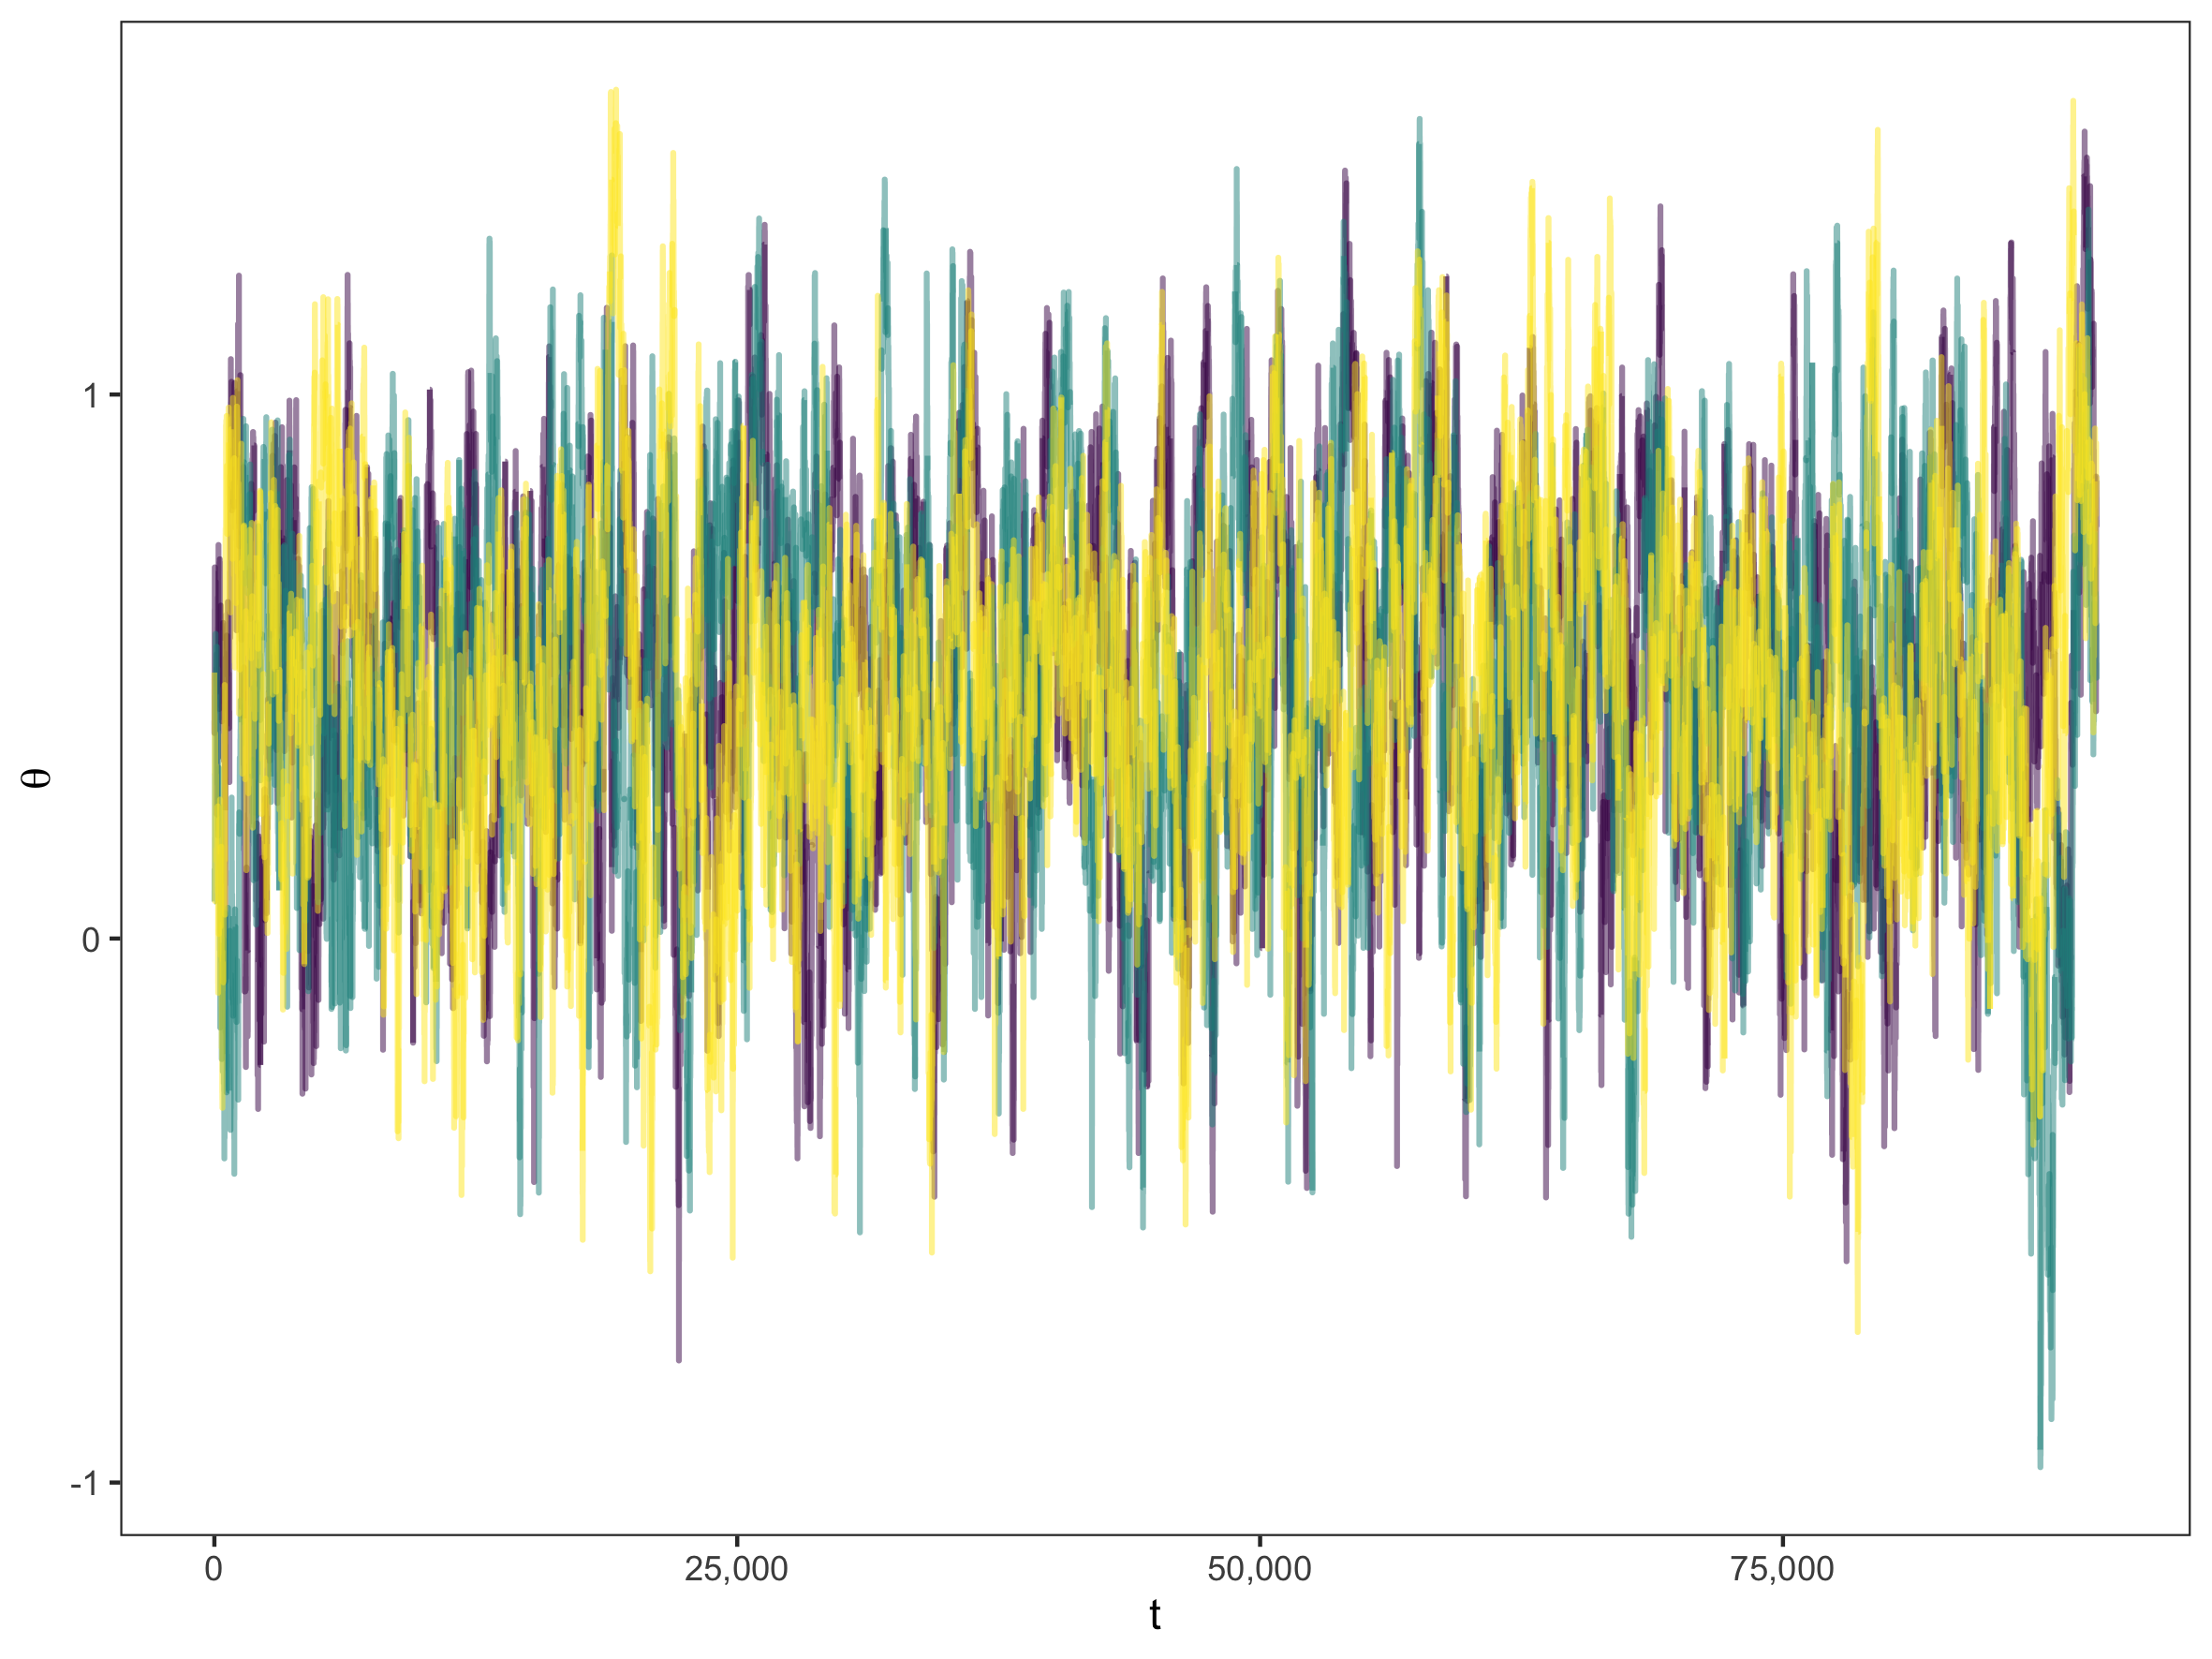
\includegraphics[width=\linewidth]{theta_traceplot.png}
       \caption{Observaciones simuladas de $\theta$.}
       \label{fig:theta_trace}
    \end{subfigure}
    \hfill
    \begin{subfigure}[t]{0.45\textwidth}
       \centering\includegraphics[width=\linewidth]{theta_ergodic_means.png}
      \caption{Evolución de $E \left[ \theta | datos \right]$ en cada iteración.}
       \label{fig:theta_means}
    \end{subfigure}

    \vspace{0.2cm}
    \begin{subfigure}[t]{\textwidth}
    \centering\includegraphics[width=\linewidth]{theta_densities.png}
    \caption{Suavizamiento con kernel gaussiano para $\pi (\theta | datos)$.}
    \label{fig:theta_densities}
    \end{subfigure}
     \caption{Diagnósticos para el parámetro $\theta$. }
    \label{fig:theta}
\end{figure}

Se podrían realizar diagnósticos para todos los parámetros involucrados en el modelo. Sin embargo, lo presentado en esta sección basta para ejemplificar el modelo de \citet{nieto} y su implementación.

\clearpage
\newpage

\subsection{Contribución al paquete \texttt{BGPhazard}}

Para cerrar este capítulo se habla un poco sobre las aportaciones que se hicieron al paquete \texttt{BGPhazard} de \citet{bgphazard}. Para crear o contribuir a un paquete no solamente se tienen que programar las funciones, además se debe documentar correctamente el paquete y cada una de las funciones, crear pruebas automatizadas para probar que todo funciona como debe y asegurarse de que los mensajes de error que arroja el paquete sean informativos para el usuario. La documentación completa de las funciones se puede consultar en CRAN\footnote{\url{https://cran.r-project.org/web/packages/BGPhazard/index.html}} o en R con el comando \texttt{help()} o `\texttt{?}'. Las funciones que se añadieron a \texttt{BGPhazard} fueron las siguientes:

\begin{itemize}
\item \texttt{BSBInit.} Se utiliza para leer tablas o vectores de datos. Extrae los tiempos de falla, indicadores de censura y variables explicativas, crea la partición del espacio de tiempo y se especifican los parámetros $\alpha$, $\beta$ y $c$ de la sección \ref{sec:ini_post}.
\item \texttt{BSBHaz.} Se utiliza para obtener simulaciones de la distribución posterior de los parámetros utilizando el muestreador de GIbbs. Se pueden modificar los intervalos de las caminatas aleatorias para parámetros que se simulan con el algoritmo de Metrópolis-Hastings.
\item \texttt{BSBPlotSumm.} Se utiliza para graficar el valor esperado y un intervalo de 0.95 de probabilidad de las tasas de riesgo $(\lambda_1, \lambda_2)$ y las funciones de supervivencia $(S_1, S_2)$.
\item \texttt{BSBPlotDiag.} Se utiliza para graficar los diagnósticos (traza y convergencia de los valores esperados) de las observaciones simuladas con la función \texttt{BSBHaz.} 
\item \texttt{BSBSumm.} Se utiliza para obtener una tabla con los valores esperados y los extremos de un intervalo de 0.95 de probabilidad para $\omega_j, \lambda_j, S_j, \gamma$ y $\theta$ $(j\in \lbrace 1, 2 \rbrace)$.
\end{itemize}

\clearpage
\newpage

\section{Conclusión}

En la introducción se menciona que los objetivos al escribir este trabajo fueron introducir al lector al modelo de supervivencia bivariado de \citet{nieto} y agregar la implementación al paquete \texttt{BGPhazard} de \citet{bgphazard}. Para cumplir con estos objetivos se presentaron las bases teóricas sobre análisis de supervivencia en el capítulo \ref{analisis_sup}, sobre cópulas e inferencia bayesiana en el capítulo \ref{cap:cop} y sobre métodos de simulación en el capítulo \ref{simulacion}. Una vez establecidas estas bases, se explicaron el modelo de \citet{nieto} y algunos detalles de la implementación en el capítulo \ref{elmodelo}.

A pesar de que se cumplieron los objetivos establecidos, todavía existen áreas de oportunidad para que el lector interesado se involucre. Por un lado, como se menciona en el capítulo \ref{elmodelo}, el modelo de \citet{nieto} solamente permite modelar correlaciones positivas entre las variables latentes $\omega_1$ y $\omega_2$, por lo que un posible trabajo de investigación sería introducir una distribución gamma bivariada que permita modelar correlaciones negativas, idealmente a través de una cópula.  Por otro lado, los algoritmos de Monte Carlo Hamiltoniano mencionados en la sección \ref{sec_cadenas} pueden ser una alternativa útil al muestreador de Gibbs, ya que el modelo cuenta con una gran cantidad de parámetros y estos algoritmos ayudan a explorar las distribuciones posteriores de manera más eficiente.

En términos de la implementación, el paquete \texttt{BGPhazard} se puede extender con funciones adicionales que los usuarios requieran, por ejemplo, incluyendo una función para generar observaciones de la distribución predictiva de la sección \ref{sec:predict} o permitiendo incorporar algunos hiperparámetros del modelo como parámetros en el muestreador de Gibbs. Se alienta al lector a que contribuya con el desarrollo del paquete \texttt{BGPhazard}. Como se menciona en la introducción, una manera sencilla de hacerlo es informando problemas o haciendo recomendaciones a través de Github.

En este trabajo no se habló con mucho detalle de las decisiones que se tomaron al momento de escribir las funciones en R y del proceso que se sigue para desarrollar un paquete. La manera de programar puede afectar para bien o para mal la velocidad de las simulaciones. El lector principiante en R puede aprender más sobre el lenguaje y sus funciones en \citet{rfordatascience}. Si ya se cuenta con experiencia en R y se desea conocer más a fondo el lenguaje y leer sobre técnicas de programación, se recomienda consultar \citet{advanced_r}. Finalmente, si el lector está interesado en cómo escribir y publicar paquetes, o en contribuir a paquetes ya existentes, se recomienda consultar \citet{rpackages}. El software libre como R y sus paquetes sobrevive y crece únicamente por el uso y la contribución de cualquier persona, sin importar su grado de estudio, intereses profesionales o áreas de investigación.

\newpage

\appendixtitleon
\appendixtitletocon
\begin{appendices}
\section{Densidad de una cópula} \label{densidad_copula}

Sean $X$ y $Y$ dos variables aleatorias continuas con función de distribución conjunta $F$ y marginales $F_X$ y $F_Y$. El teorema de Sklar (\ref{sklar}) dice que existe una única cópula $C$ tal que $$F(x, y) = C(F_X(x), F_Y(y)).$$

\begin{proposition}
Bajo las condiciones del Teorema de Sklar, la densidad conjunta de $X$ y $Y$, denotada $f$, está dada por $$\frac{\partial^2 F}{\partial y \partial x} = c(F_X(x), F_Y(y))f_X(x)f_Y(y),$$ donde $c$ es la densidad de la cópula $C$, $f_X$ es la densidad marginal de $X$ y $f_Y$ la densidad marginal de $Y$.
\end{proposition} 

\begin{proof}
\begin{align*}
\frac{\partial F}{\partial x} &= \frac{\partial C(F_X(x), F_Y(y))}{\partial x}\\
&= \frac{\partial C}{\partial F_X} \frac{\partial F_X}{\partial x}\\
&= \frac{\partial C}{\partial F_X}f_X(x)\\
\frac{\partial F}{\partial y \partial x} &= \frac{\partial}{\partial y} \left[\frac{\partial C}{\partial F_X}f_X(x)\right]\\
&= \frac{\partial C}{F_Y F_X}\frac{\partial F_Y}{\partial y}f_X(x)\\
&= c (F_X(x), F_Y(y)) f_X(x) f_Y(y).
\end{align*}
\end{proof}

La notación $dC(u, v)$ se refiere a la integral de Riemann-Stieltjes, una generalización de la integral de Riemann que se utiliza en la teoría de probabilidad para homologar notación entre distribuciones continuas y discretas. Si la función $F$ es una función de distribución continua con función de densidad $f(x) = \frac{d}{dx}F(x)$, $f(x) > 0 \ \forall x \in S_X$, se tiene que $$\int f(x) dx = \int dF(x)$$ (ver \citet{rudin}[p. 131]).

Si una cópula $C$ tiene densidad dada por $\frac{\partial ^2}{\partial v \partial u} C(u, v)$, entonces $C$ es absolutamente continua (ver \citet{nelsen}[p. 23]), por lo que $$\int\int \ dC(u,v) = \int\int  c(u, v) \ dudv.$$

Para mayor información sobre integrales de Riemann-Stieltjes ver \citet{rudin} y \citet{bartle}.

\newpage

\section{Axiomas de coherencia y probabilidad subjetiva} \label{ap:bayes}

\textbf{Axioma de comparabilidad.} Para todo par de elementos $d_1, d_2 \in \mathcal{D}$, es cierta una y solamente una de las siguientes:
\begin{itemize}
\item Se prefiere $d_1$ sobre $d_2$, denotado $d_1 \succ d_2$.
\item  Se prefiere $d_2$ sobre $d_1$, denotado $d_2 \succ d_1$.
\item Se prefieren igual $d_1$ y $d_2$, denotado $d_1 \sim d_2$.
\end{itemize}
Además, existen $c_*, c^*$ tales que $c_* \preceq c \preceq c^*$ $\forall c \in C$.

\textbf{Axioma de transitividad.} $\forall d_1, d_2, d_3 \in \mathcal{D}$, $d_1 \succ d_2$ y $d_2 \succ d_3$ $\implies$ $d_1 \succ d_3$.

\textbf{Axioma de sustituibilidad.} Si $E$ es un evento incierto y $d_1, d_2$ son decisiones tales que $d_1 \succ d_2$ cuando sucede $E$ y $d_1 \succ d_2$ cuando sucede $E^c$, entonces $d_1 \succ d_2$. De la misma forma, si $d_1 \sim d_2$ bajo $E$ y $d_1 \sim d_2$ bajo $E^c$, entonces $d_1 \sim d_2$.

\textbf{Axioma de eventos de referencia.} El tomador de decisiones puede imaginar un procedimiento para generar puntos en el cuadrado unitario $I = [0, 1] \times [0, 1]$ de manera que para dos regiones $R_1, R_2 \subset I$, el evento $\lbrace r \in R_1\rbrace$ es más creíble que el evento $\lbrace r \in R_2 \rbrace$ si y solamente si $A(R_1) > A(R_2)$, donde $A$ se refiere al área de la región.

Al plantear un problema de decisión, \citet{mendoza} sugieren añadir al conjunto de decisiones $\mathcal{D}$ las opciones $d_c = \lbrace c|\Omega\rbrace$ $\forall c \in C$, $d_E = \lbrace c_* | E^c, c^* | E \rbrace$ $\forall E \subset \mathcal{E}$ y $d_R = \lbrace c_*|R^c, c^* | R\rbrace$ $\forall R \subset I$.  Por facilidad de notación, se seguirá utilizando $\mathcal{D}$ para referirse al conjunto de decisiones extendido. Es importante notar que con estas extensiones también se puede hablar indistintamente de preferencias sobre las consecuencias o sobre las decisiones, ya que si se tienen $c_1, c_2 \in C$, se dice que $c_1 \succ c_2$ si y solamente si $d_{c_1} \succ d_{c_2}$.

\textbf{Axioma de densidad.} Para todo $d \in \mathcal{D}$ existe $R \subset I$ tal que $d \sim d_R$.

Una vez establecido este axioma, \citet{mendoza} definen la probabilidad subjetiva de un evento relevante $E \in \mathcal{E}$ bajo las condiciones $H$ como $P(E|H) = A(R)$, donde $R$ es tal que $d_R \sim d_E$ bajo las condiciones $H$ y $A(R)$ denota el área de $R$. Los autores demuestran que $P(E|H)$ existe y es única para todo evento relevante $E \in \mathcal{E}$ y también demuestran que esta probabilidad subjetiva cumple con los axiomas de Kolmogorov como consecuencia de los axiomas de coherencia:
\begin{enumerate}
\item $0 \leq P(E|H) \leq 1$.
\item $P(\emptyset|H) = 0$.
\item $P(\Omega | H) = 1$.
\item $E\cap F = \emptyset \implies P(E\cup F|H) = P(E|H) + P(F|H)$.
\end{enumerate}

\newpage

\section{Construcción de la cópula} \label{construccion_copula}

En este apéndice se hace referencia a la ecuación \eqref{copula_modelo} de la sección \ref{elmodelo}. Del caso univariado \eqref{mezcla} se obtiene la expresión para las funciones de distribución marginales:
\begin{align*}
F(t) &= \int_0^t f(s) \ ds\\
&= \int_0^t\left(\int_0^\infty f(s|\omega)m(\omega) \ d\omega \right) \ ds\\
&= \int_0^t h(s)e^{-H(s)} \ ds\\
&= \int_0^{H(t)} e^{-u} \ du\\
&= 1-e^{-H(t)},
\end{align*}
por lo que, en el caso bivariado,
\begin{equation}\label{dist_marginal}
F_j(t) = 1-e^{-H_j(t)}.
\end{equation}

De las ecuaciones \eqref{mezcla_conjunta} y \eqref{indcon} se obtiene $$f(t_1, t_2) = \int_{H_1(t_1)}^\infty \int_{H_2(t_2)}^\infty \frac{h_1(t_1)}{\omega_1}\frac{h_2(t_2)}{\omega_2}m(\omega_1, \omega_2) \ d\omega_2 d\omega_1,$$ de donde se puede calcular la función de distribución conjunta $F(t_1, t_2)$.
\begin{align*}
F(t_1, t_2) &= \int_0^{t_1} \int_0^{t_2} f(s_1, s_2) \ ds_1 ds_2\\
&= \int_0^{t_1} \int_0^{t_2}\int_{H_1(s_1)}^\infty \int_{H_2(s_2)}^\infty \frac{h_1(s_1)}{\omega_1}\frac{h_2(s_2)}{\omega_2}m(\omega_1, \omega_2) \ d\omega_2 d\omega_1\\
= \int_0^{t_1}\int_{H_1(s_1)}^\infty &\frac{h_1(s_1)}{\omega_1}\left(\int_0^{t_2} \int_{H_2(s_2)}^\infty \frac{h_2(s_2)}{\omega_2} m(\omega_1, \omega_2) \ d\omega_2 ds_2 \right) d\omega_1 ds_1.
\end{align*}

Para desarrollar $$I_1 = \int_0^{t_2} \int_{H_2(s_2)}^\infty \frac{h_2(s_2)}{\omega_2} m(\omega_1, \omega_2) \ d\omega_2 ds_2$$ cambiando el orden de integración se obtiene
\begin{align*}
I_1 &= \int_0^{H_2(t_2)}\int_0^{H_2^{-1}(\omega_2)} \frac{h_2(s_2)}{\omega_2}m(\omega_1, \omega_2) \ ds_2 d\omega_2 \ +\\
& \ \ \ \int_{H_2(t_2)}^\infty \int_0^{t_2} \frac{h_2(s_2)}{\omega_2}m(\omega_1, \omega_2) \ ds_2 d\omega_2\\
&= \int_0^{H_2(t_2)} m(\omega_1, \omega_2) \ d\omega_2 \ + \ \int_{H_2(t_2)}^\infty \frac{H_2(t_2)}{\omega_2}m(\omega_1, \omega_2) \ d\omega_2.
\end{align*}

Ahora
\begin{align*}
&m(\omega_1) = \int_0^\infty m(\omega_1, \omega_2) \ d\omega_2\\
&= \int_0^{H_2(t_2)} m(\omega_1, \omega_2) \ d\omega_2 \ + \ \int_{H_2(t_2)}^\infty m(\omega_1, \omega_2) \ d\omega_2\\
&\implies \int_0^{H_2(t_2)} m(\omega_1, \omega_2) \ d\omega_2 = m(\omega_1) - \int_{H_2(t_2)}^\infty m(\omega_1, \omega_2) \ d\omega_2\\
&\implies I_1 = m(\omega_1) + \int_{H_2(t_2)}^\infty m(\omega_1, \omega_2) \left( \frac{H_2(t_2)}{\omega_2}-1\right) \ d\omega_2,
\end{align*}
por lo que, regresando a $F(t_1, t_2)$ se tiene que

\begin{align*}
F(&t_1, t_2) = \int_0^{t_1} \int_{H_1(s_1)}^\infty \frac{h_1(s_1)}{\omega_1}\left( I_1 \right) \ d\omega_1 ds_1\\
&= \int_0^{t_1} \frac{h_1(s_1)}{\omega_1}m(\omega_1) \ d\omega_1 ds_1 \ +\\ & \ \ \ \int_{H_2(t_2)}^\infty \left(\frac{H_2(t_2)}{\omega_2}-1 \right) \left(\int_0^{t_1}\int_{H_1(s_1)}^\infty \frac{h_1(s_1)}{\omega_1}m(\omega_1, \omega_2) \ d\omega_1 ds_1 \right) d\omega_2\\
&= F_1(t_1) \ + \\
& \ \ \ \int_{H_2(t_2)}^\infty \left(\frac{H_2(t_2)}{\omega_2}-1 \right)\left(m(\omega_2) + \right.\\
\ \ \ \ \ \ &\left.  \int_{H_1(t_1)}^\infty m(\omega_1, \omega_2) \left(\frac{H_1(t_1)}{\omega_1}-1 \right) \ d\omega_1 \right) d\omega_2\\
&= F_1(t_1) \ + \ \int_{H_2(t_2)}^\infty m(\omega_2) \left( \frac{H_2(t_2)}{\omega_2}-1 \right) \ d\omega_2 \ +\\
& \ \ \ \int_{H_2(t_2)}^\infty\int_{H_1(t_1)}^\infty \left(\frac{H_2(t_2)}{\omega_2}-1\right)\left(\frac{H_1(t_1)}{\omega_1}-1\right) m(\omega_1, \omega_2) \ d\omega_1 d\omega_2\\
&= F_1(t_1) + F_2(t_2) - 1 \ +\\
& \ \ \ \int_{H_2(t_2)}^\infty\int_{H_1(t_1)}^\infty \left(\frac{H_2(t_2)}{\omega_2}-1\right)\left(\frac{H_1(t_1)}{\omega_1}-1\right) m(\omega_1, \omega_2) \ d\omega_1 d\omega_2.
\end{align*}

Como $H_j(t_j) = -\log (1-F_j(t_j))$, entonces se tiene que la función de distribución conjunta cumple $F(t_1, t_2) = C(F_1(t_1), F_2(t_2))$, donde $C$ es la función dada por
\begin{align*}
C(&u, v) = u \ + \ v \ - \ 1 \ + \nonumber \\
&\int_{-\log (1-u)}^\infty \int_{-\log (1-v)}^\infty\\
&\ \ \ \ \left( \frac{\log (1-u)}{\omega_1}+1 \right) \left( \frac{\log (1-v)}{\omega_2}+1\right) m(\omega_1, \omega_2) \ d\omega_2 d\omega_1.
\end{align*}

Para obtener la cópula de supervivencia \eqref{copula_modelo}, se utiliza el resultado \ref{def_cop_surv} y se concluye que $$S(t_1, t_2) = \widehat{C}(S_1(t_1), S_2(t_2)),$$ donde $\widehat{C}$ es la función dada por
\begin{align*}
\widehat{C}(&u, v) =\\
&\int_{-\log (u)}^\infty \int_{-\log (v)}^\infty \left( \frac{\log (u)}{\omega_1}+1 \right) \left( \frac{\log (v)}{\omega_2}+1\right) m(\omega_1, \omega_2) \ d\omega_2 d\omega_1.
\end{align*}

\newpage

\section{Densidad de la cópula del modelo}
\label{sec_densidad_copula_modelo}

Se quiere obtener la densidad de la cópula \eqref{copula_distribucion}. Para esto se utiliza la regla de Leibniz para la derivada de una integral. Esta regla es:
\begin{align}\label{regla_leibniz}
\frac{d}{dx} \int_{a(x)}^{b(x)} f(x, t) \ dt &= f(x, b(x)) \frac{d}{dx}b(x) \ - \ f(x, a(x))\frac{d}{dx}a(x) \ + \nonumber\\
&\ \ \ \int_{a(x)}^{b(x)}\frac{\partial}{\partial x} f(x, t) \ dt
\end{align}
Los supuestos y la demostración se pueden encontrar en \citet{flanders}.

La expresión para la cópula \eqref{copula_distribucion} es
\begin{align*}
C(u, v) &= u \ + \ v \ - \ 1 \ +\\ 
& \ \ \ \int_{-\log (1-u)}^\infty \int_{-\log (1-v)}^\infty f(u, v, \omega_1, \omega_2) \ d\omega_2 d\omega_1,
\end{align*}
donde $f(u, v, \omega_1, \omega_2) = \left( \frac{\log (u)}{\omega_1}+1 \right) \left( \frac{\log (v)}{\omega_2}+1\right) m(\omega_1, \omega_2)$.

Aplicando \eqref{regla_leibniz} se tiene que
\begin{align*}
\frac{\partial C}{\partial u} &= 1 + \frac{\partial}{\partial u} \int_{-\log (1-u)}^\infty g_1(u, v, \omega_1, \omega_2) \ d\omega_1\\
&= 1 \ - \ g_1(u, v, -\log (1-u), \omega_2)\frac{\partial}{\partial u}\left[ -\log (1-u) \right] \ +\\
& \ \ \ \int_{-\log (1-u)}^{\infty} \frac{\partial}{\partial u}g_1(u, v, \omega_1, \omega_2) \ d\omega_1\\
&= \int_{-\log (1-u)}^\infty \int_{-\log (1-v)}^\infty \left(-\frac{1}{(1-u)\omega_1}\right)\left(1+\frac{\log (1-v)}{\omega_2}\right)\\
&\ \ \ \ m(\omega_1, \omega_2) \ d\omega_2 d\omega_1,
\end{align*}
donde
\begin{align*}
g_1(&u, v, \omega_1, \omega_2) =\\
&\int_{-\log (1-v)}^\infty \left(1+\frac{\log (1-u)}{\omega_1}\right)\left(1+\frac{\log (1-v)}{\omega_2}\right) m(\omega_1, \omega_2) \ d\omega_2
\end{align*}
y $$g_1(u, v, -\log (1-u), \omega_2) = 0.$$

Así, aplicando otra vez \eqref{regla_leibniz} se tiene que
\begin{align*}
&\frac{\partial C^2}{\partial v \partial u} = \frac{\partial}{\partial v} \int_{-\log (1-v)}^\infty g_2(u, v, \omega_1, \omega_2) \ d\omega_2\\
&= -g_2(u, v, \omega_1, -\log (1-v))\frac{\partial}{\partial v}\left[ -\log (1-v)\right] \ +\\
&\ \ \ \int_{-\log (1-v)}^\infty \frac{\partial}{\partial v}g_2(u, v, \omega_1, \omega_2) \ d\omega_2\\
&= \int_{-\log (1-u)}^\infty \int_{- \log (1-v)}^\infty \left(\frac{1}{(1-u)\omega_1}\right)\left(\frac{1}{(1-v)\omega_2}\right) m(\omega_1, \omega_2) \ d\omega_2 d\omega_1.
\end{align*}
Por lo que
\begin{align*}
c&(u, v) =\\
&\int_{-\log (1-u)}^\infty \int_{- \log (1-v)}^\infty \left(\frac{1}{(1-u)\omega_1}\right)\left(\frac{1}{(1-v)\omega_2}\right) m(\omega_1, \omega_2) \ d\omega_2 d\omega_1.
\end{align*}

\newpage

\section{Códigos de R}
\subsection{Ejemplo de verosimilitud exponencial}
\label{ap:lik}

\begin{table}[!htb]
\begin{lstlisting}
nsim <- 10000
lambda <- 0.1

set.seed(42)

time.samples <- rexp(n = nsim, rate = lambda)

# Suponemos que el monitoreo termino en T = 15

time.censored <- ifelse(time.samples > 15, 15, time.samples)
delta <- ifelse(time.samples > 15, 0, 1)

log_lik <- function(lambda) {
  sum(delta) * log(lambda) - lambda * sum(time.censored)
}

log_lik_exact <- function(lambda) {
  length(time.censored) * log(lambda) - lambda * sum(time.censored)
}

time.drop <- time.censored[delta == 1]

log_lik_drop <- function(lambda) {
  length(time.drop) * log(lambda) - lambda * sum(time.drop)
}

max.ver1 <- sum(delta) / sum(time.censored)
max.ver2 <- 1 / mean(time.censored)
max.ver3 <- 1 / mean(time.drop)

ymin <- log_lik(0.01)

curve(
  log_lik,
  from = 0.01,
  to = 0.3,
  ylim = c(ymin, log_lik_drop(max.ver3)),
  xlab = expression(lambda),
  ylab = "",
  yaxt = 'n',
  col = "steelblue"
  )
curve(log_lik_exact, from = 0.01, to = 0.3, add = TRUE, col = "forestgreen")
curve(log_lik_drop, from = 0.01, to = 0.3, add = TRUE, col = "darkorange")
lines(x = c(max.ver1, max.ver1), y = c(ymin, log_lik(max.ver1)), lty = 2, col = "steelblue")
lines(x = c(max.ver2, max.ver2), y = c(ymin, log_lik_exact(max.ver2)), lty = 2, col = "forestgreen")
lines(x = c(max.ver3, max.ver3), y = c(ymin, log_lik_drop(max.ver3)), lty = 2, col = "darkorange")
abline(
  v = 0.1,
  col = "gray80",
  lty = 2)
\end{lstlisting}
\caption{Código para reproducir el ejemplo de la sección \ref{sec:ver} en R.}
\end{table}

\newpage
\clearpage

\subsection{Funciones \texttt{partition\_location} y \texttt{partition\_count}}
\label{ap:partition_functions}

\begin{table}[!htb]
\begin{lstlisting}
# Returns the interval of the partition in which t is located.

partition_location <- function(t, partition) {

  lt <- length(t)
  t_loc <- rep(0, times = lt)

  for (i in 1:lt) {
    j <- 1
    while(t[i] > partition[j + 1] & j < length(partition)) {
      j <- j + 1
    }
    t_loc[i] <- j
  }

  return(t_loc)

}
\end{lstlisting}
\caption{Código para definir la función \texttt{partition\_location} de la sección \ref{sec:ini_post}.}
\end{table}

\begin{table}[!htb]
\begin{lstlisting}
# Count how many failure times are in each interval of partition
partition_count <- function(t, partition) {
  t_loc <- partition_location(t, partition)
  counts <- rep(0, times = (length(partition) - 1))

  for (i in 1:length(counts)) {
    counts[i] <- sum(t_loc == i)
  }

  return(counts)

}
\end{lstlisting}
\caption{Código para definir la función \texttt{partition\_count} de la sección \ref{sec:ini_post}.}
\end{table}

\end{appendices}

\clearpage
\newpage

\bibliography{tesis_bibliografia}

\end{document}
